\documentclass[14pt, letterpaper, openany]{book}

% Use of Bulgarian language.
\usepackage[T2A, T1]{fontenc}
\usepackage[utf8]{inputenc}
\usepackage[english]{babel}

% Used to group images.
\usepackage{subcaption}

% Using the graph.
\usepackage[pdftex]{graphicx}

% Use more precise positions for the images.
\usepackage{float}

% Using PDFs for covers.
\usepackage{pdfpages}

% Using header and footer.
\usepackage{fancyhdr}

% Use quotation marks when quoting.
%\usepackage{dirtytalk}
\usepackage{csquotes}

% Used to create an alphabetical index.
\usepackage{imakeidx}

% Adds the possibility of sensitive hyperlinks in the document itself.
\usepackage[pdftex, bookmarks, linktocpage]{hyperref}

% A command with many options for setting the behavior of the hyperref package, with the most useful option being the Cyrillicization of titles from Bookmarks in Acrobat.
\hypersetup{unicode=true, colorlinks=true, linkcolor=black, citecolor=black, urlcolor=black}

% Used for listings with program code.
\usepackage{listings}

% Used for multiline comments.
\usepackage{verbatim}

% Used for line spacing.
\usepackage{lipsum}

% Used for tables that span more than one page.
\usepackage{longtable}

% Title.
\title{Block Programming with Scratch and App Inventor}

% Authors.
\author{Todor Balabanov, Galya Petrova, Antonia Guzgunova}

% Directory with images.
\graphicspath{{images/}}

% Select active language.
\selectlanguage{english}

% Texts to decorate the page at the top and bottom.
\pagestyle{fancy}
\fancyhf{}
\fancyhead[LE,RO]{\thepage}
\fancyhead[RE]{Block Programming with Scratch and App Inventor}
\fancyhead[LO]{Todor Balabanov, Galya Petrova, Antonia Guzgunova}
\fancyfoot[LE,RO]{Publishing House ''Education and Knowledge'', 2023, Sofia}

% Thickness of dividing lines.
\renewcommand{\headrulewidth}{2pt}
\renewcommand{\footrulewidth}{1pt}

% Generate alphabetical index.
\onecolumn
\makeindex[columns=2, title=Index, intoc]

% Replaces the word a used for numbering program code fragments.
\renewcommand{\lstlistingname}{Listing}

% Change the name for the list from the listings.
%\renewcommand{\lstlistlistingname}{Listing List}

% Defines the listing characteristics for the program code.
\lstset{backgroundcolor=\color{gray!30}, breaklines=true, language=r, frame=single}

% One and a half line spacing.
\linespread{1.5}

% Start of document.
\begin{document}

% Front cover.
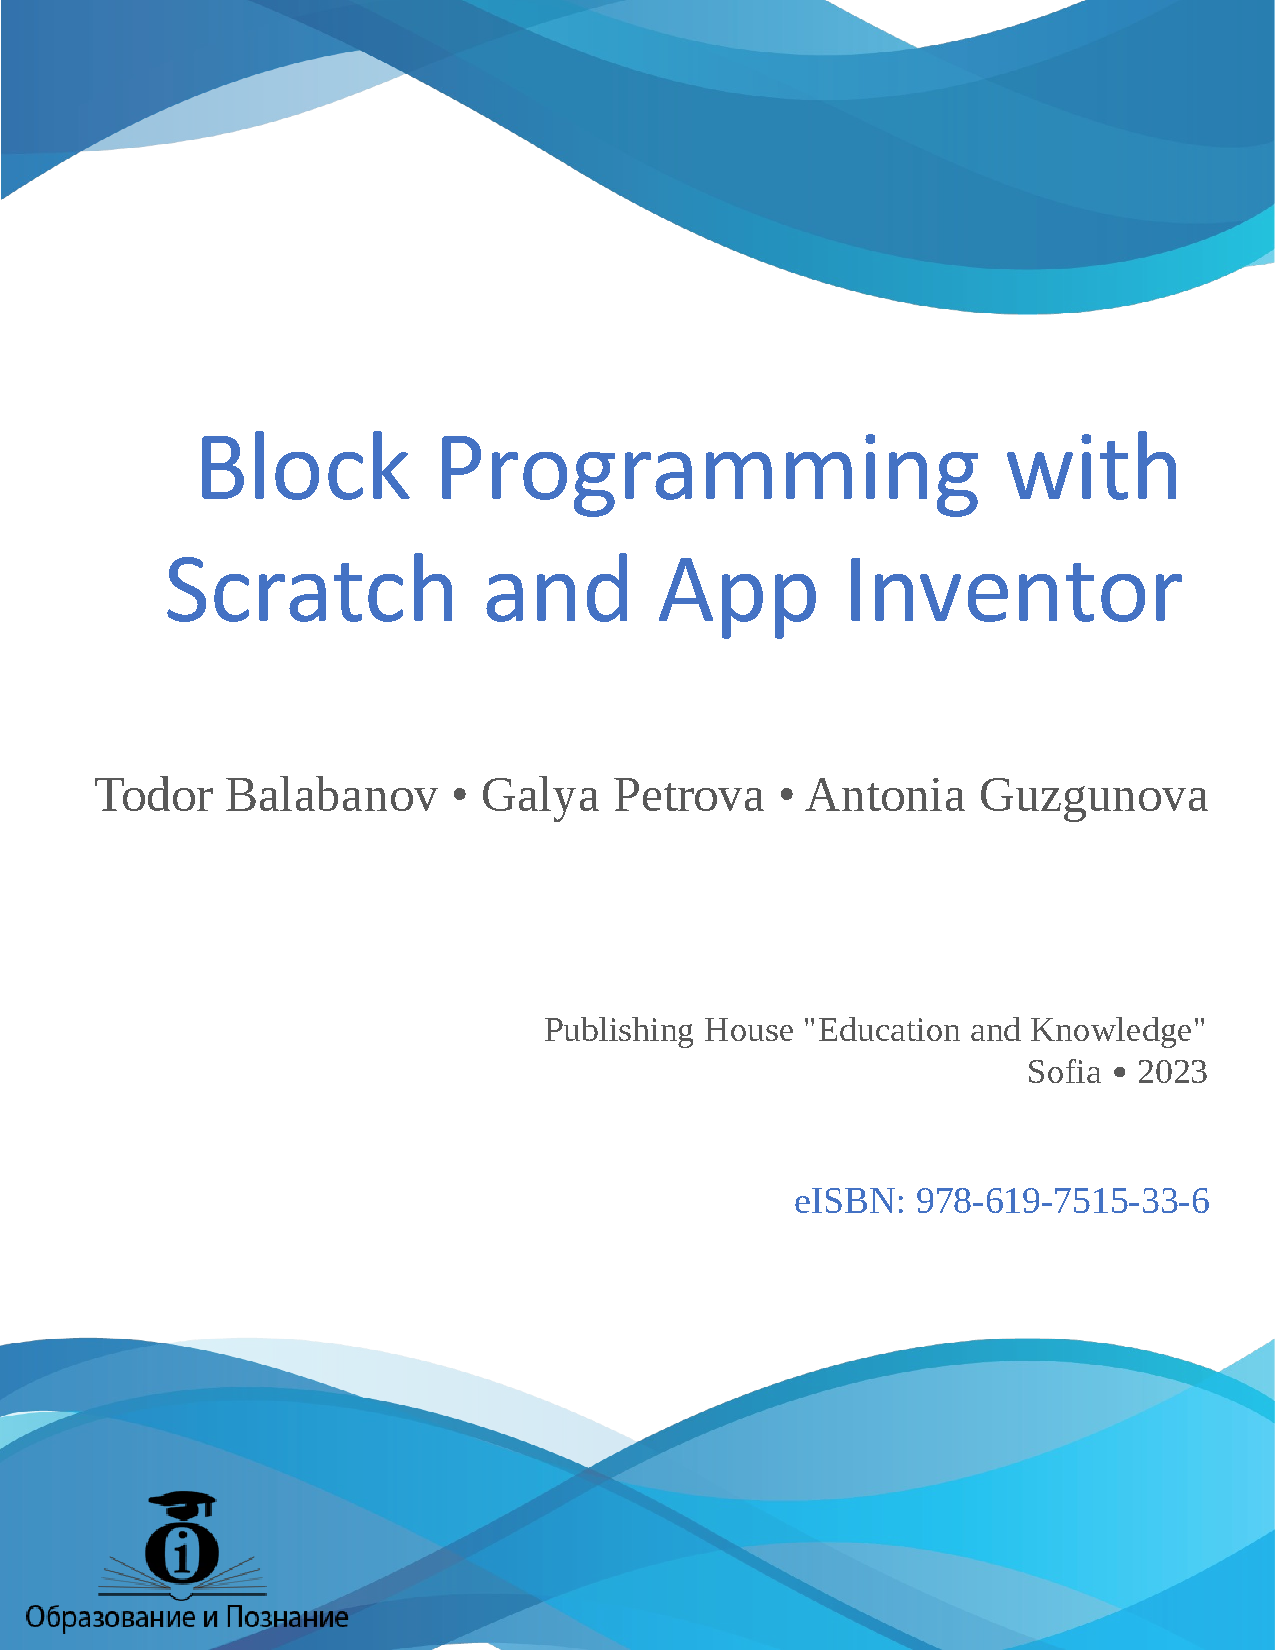
\includepdf[pages={1}]{covers-en/front}
\thispagestyle{empty}

% Copyright page.
~\vfill
\thispagestyle{empty}

\noindent Copyright \copyright\ 2023 \\

\noindent Todor Balabanov, Galya Petrova, Antonia Guzgunova \\ 

\noindent \textsc{Publishing House ''Education and Knowledge''} \\
\noindent \textsc{https://www.obrazovaniebg.net/} \\

\noindent {\footnotesize This book is supported by the Ministry of Education and Science of the Republic of Bulgaria under the National Science Program ''INTELLIGENT ANIMAL HUSBANDRY, grant agreement No. D01-62/18.03.2021''}. \\

\noindent \textit{1st Editon, 2023}



% Numbering of service information pages.
\pagenumbering{roman}
\setcounter{page}{1}

% Table of contents.
\addcontentsline{toc}{chapter}{Table of Contents}
\tableofcontents\newpage

% List of figures.
\addcontentsline{toc}{chapter}{List of Figures}
\listoffigures\newpage

% List of tables.
%\addcontentsline{toc}{chapter}{List of Tables}
%\listoftables\newpage

% List of listings.
%\addcontentsline{toc}{chapter}{List of Source Codes}
%\lstlistoflistings\newpage

% Numbering of the pages with the main exposition.
\pagenumbering{arabic}
\setcounter{page}{1}

% Individual chapters are in separate files.
%\addcontentsline{toc}{chapter}{Preface}
\chapter*{Preface}
\thispagestyle{empty}

This book is intended for all people who are excited about topics in programming and especially about teaching children in this field. We hope anyone interested in the area finds something valuable in the material presented. Our experience primarily concerns the academic world and pedagogy dedicated to children's education. The material is presented in such a way as to reveal the basic mechanisms of learning by doing. Generally speaking, the book guides the reader with minimal computer knowledge to a good understanding of programming concepts.

From our point of view, the presentation of program constructions with the help of visualization, as close as possible to classic puzzles, gives ample opportunities for learning valuable knowledge and skills. Such a visualization approach allows for an effective lowering of the programming learning age. While classical programming languages are appropriate in high school classrooms, block languages effectively find their application in the junior high school course of study.

Part of the presented material explains fundamental concepts in programming, such as - sequence of instructions, conditional and unconditional transitions, cyclicity of actions, events, modular organization, and others. Another part emphasizes practical implementation and ideas that have the potential to become independent software solutions. The chosen approach to presenting the information is through examples of the principle - do, step by step.

The book assumes no prerequisites for an advanced level of computer literacy but relies on the reader having a basic knowledge of what a computer system is, what an operating system is, what the Internet is, and how it handles loading and browsing web pages. The considered block programming systems are web-based, and work with them takes place in a cloud space. A deep knowledge of mathematics is not required, but a basic knowledge of algebra and geometry helps understand some examples. Artistic skills, such as musicality or visual arts, are unnecessary, but their presence would give additional flavor to the results achieved.

The material is organized into chapters related to each other, and for complete absorption, it is desirable to read them in the given sequence. Part of the exposition in the book is based on subjects taught in the junior high school course of study.

\vspace{0.5cm}

\large{\textbf{Acknowledgments}}

\vspace{0.5cm}

The authors would like to thank their families for their patience and understanding while writing this book. They would also like to thank their colleagues and friends who helped to achieve higher quality.

\newpage
%\chapter{Work Environments}

Block programming languages are a subdivision of visual programming languages. The essence of block languages is that program instructions are entered in the form of colored blocks and not, as in classical programming languages, by writing text commands. The most basic purpose of block languages is to make the field of programming significantly more accessible to beginners. This goal is achieved through three main directions. From a syntactic point of view, instructions in block languages are in the form of colored icons. This greatly reduces the possibility of writing the wrong program instruction. Second, semantics are improved, with each possible program instruction being well documented. In third place is pragmatism, which allows the study of the different states in which the program can fall. Block programming environments have grown in popularity over the past decade. Some of the most popular ones are Scratch, Blockly, App Inventor for Android, Ardublock, and others. This book will focus on two block programming environments created at MIT, Scratch and App Inventor for Android. This choice is because Scratch is aimed at the youngest, namely children in primary school classes, which is very well combined with the possibility to visualize the block programs on a mobile phone through App Inventor for Android. Both software environments do not require the installation of specialized software. It is enough to have a modern computer connected to the Internet and a modern web browser version.

\section{Getting Started in Scratch}

Working in the Scratch environment begins by loading the main web page (Fig. \ref{fig010001}), which is located at: \\ \href{https://scratch.mit.edu/}{https://scratch .mit.edu/}

\begin{figure}[H]
   \centering
   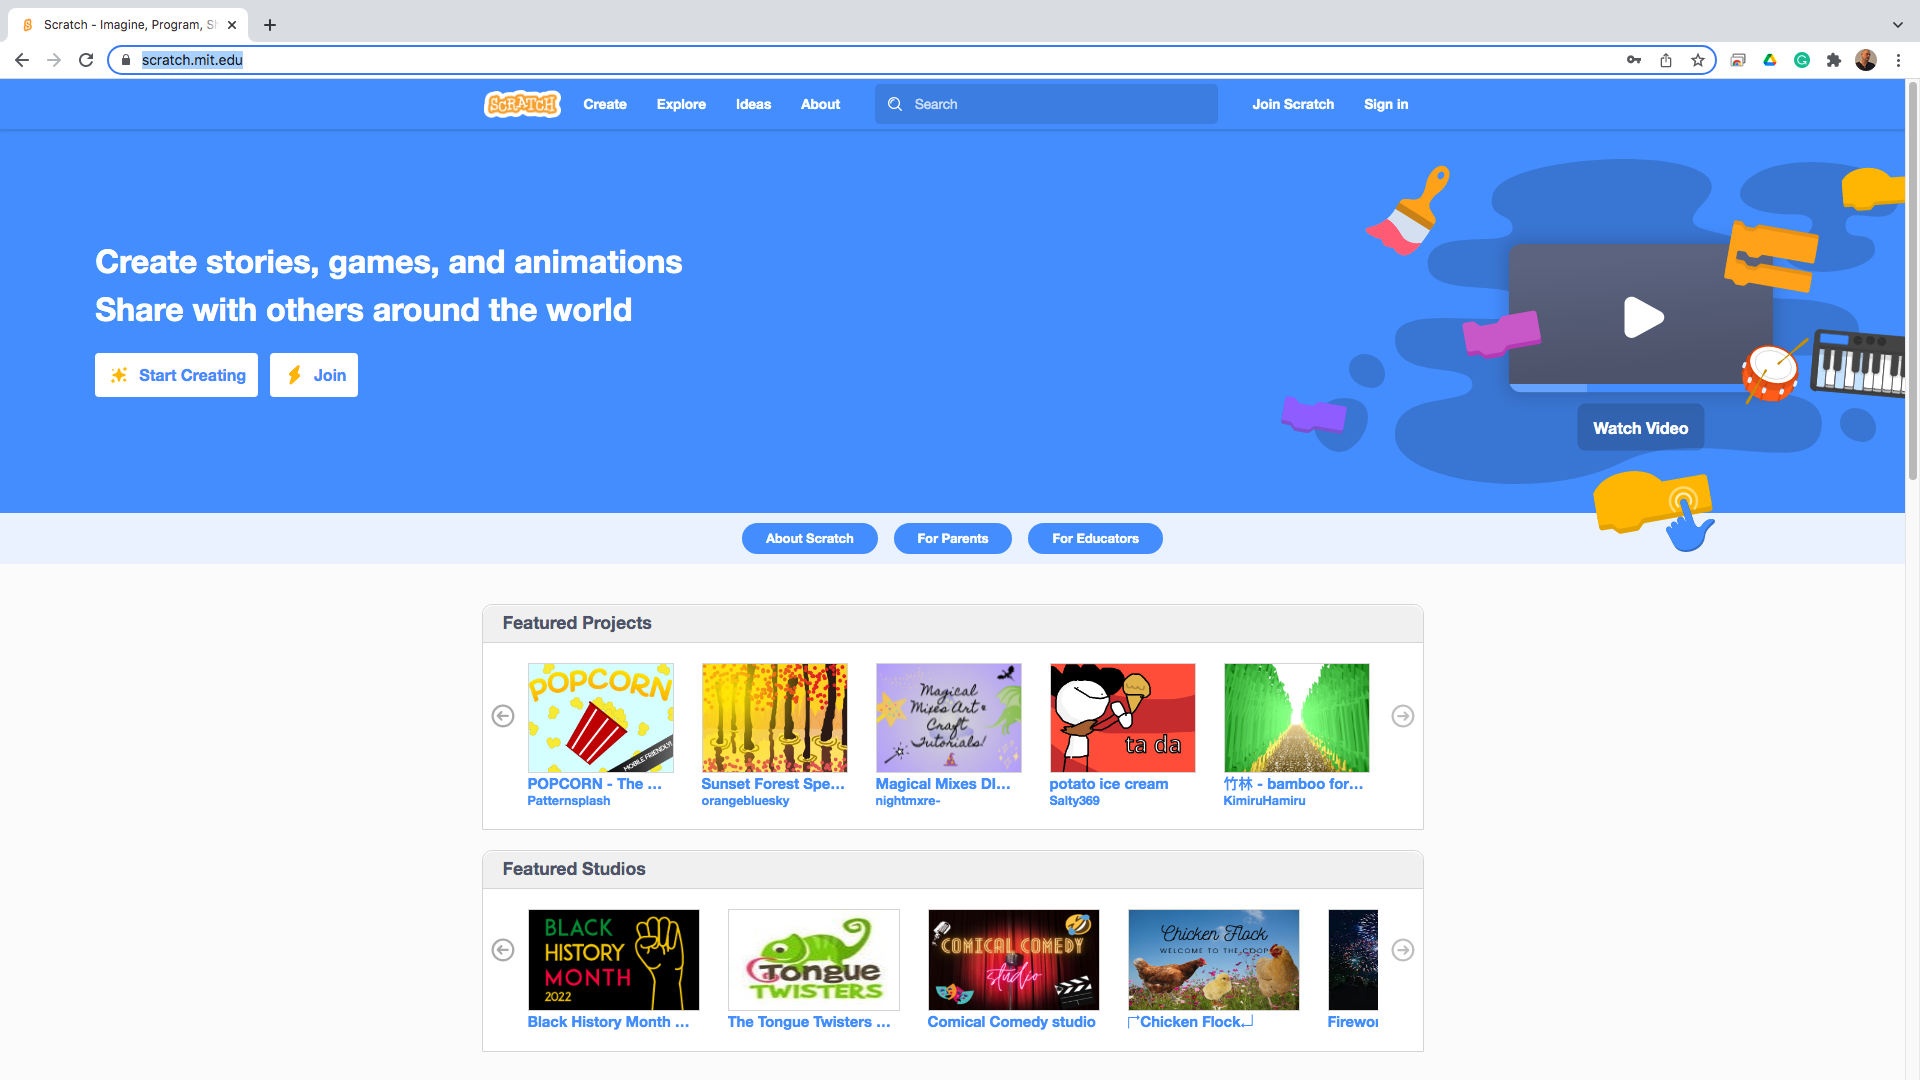
\includegraphics[width=1.0\linewidth,height=0.5\linewidth]{fig010001.png}
   \caption{Scratch Homepage}
\label{fig010001}
\end{figure}

The program environment of Scratch is organized on the principle of cloud services. For this reason, anyone wishing to use the service must register (Fig. \ref{fig010002}). The registration consists of a username and password.

\begin{figure}[H]
   \centering
   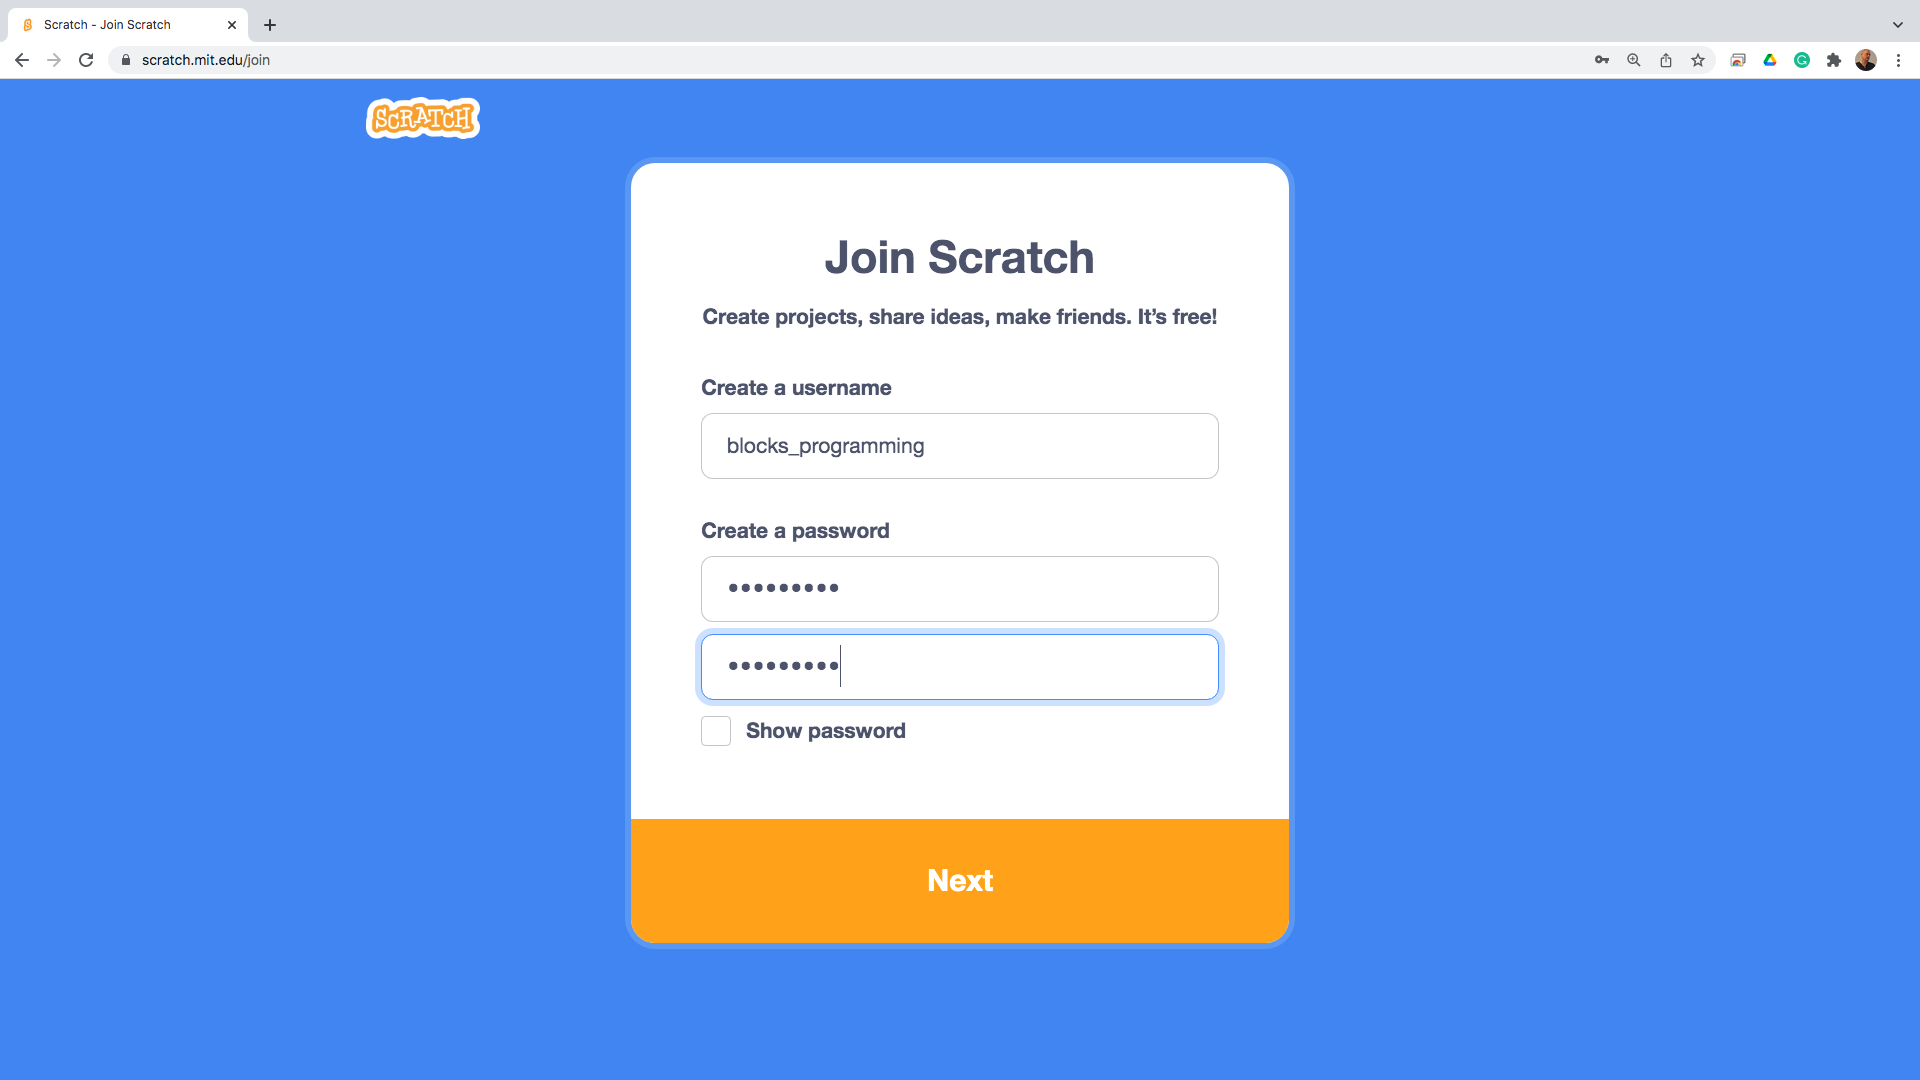
\includegraphics[width=1.0\linewidth,height=0.5\linewidth]{fig010002.png}
   \caption{Scratch user registration}
\label{fig010002}
\end{figure}

After choosing a username and password, the geographical region in which the user is located follows (Fig. \ref{fig010003}).

\begin{figure}[H]
   \centering
   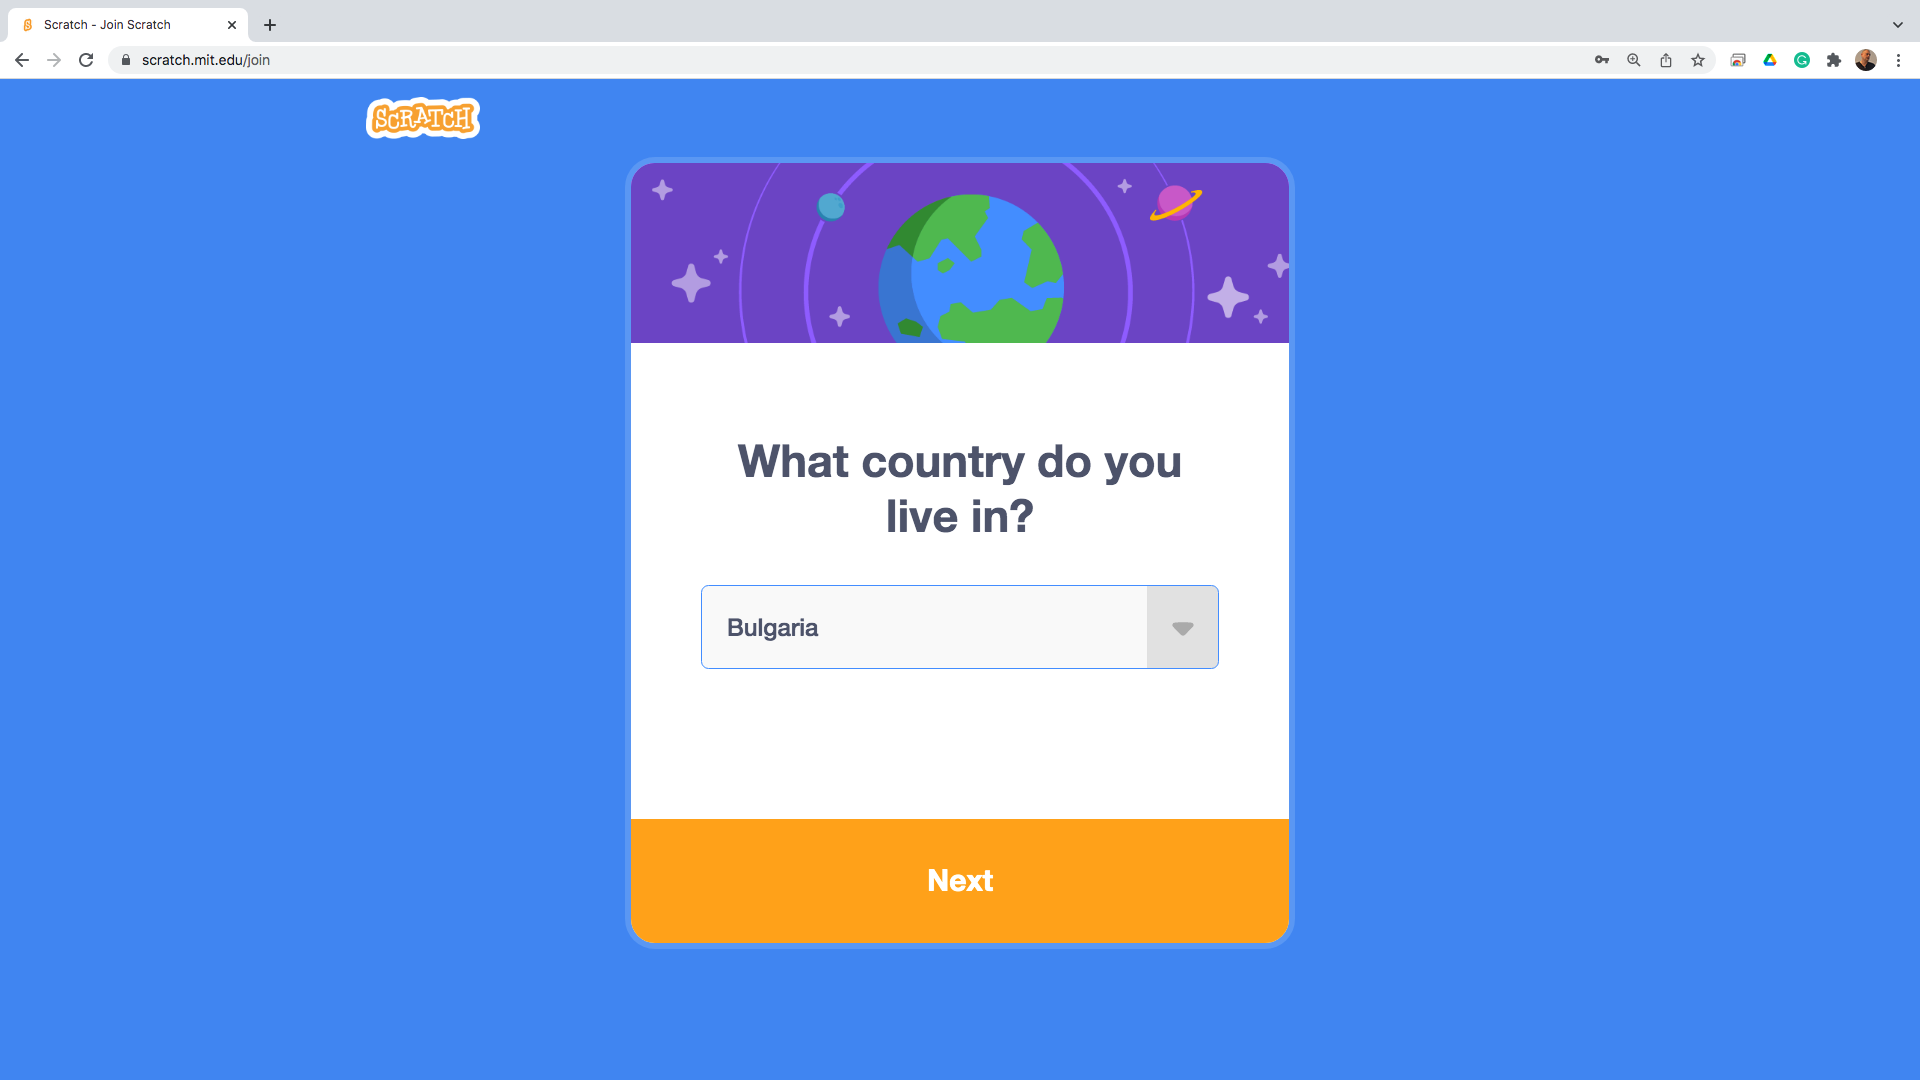
\includegraphics[width=1.0\linewidth,height=0.5\linewidth]{fig010003.png}
   \caption{Geographic location}
\label{fig010003}
\end{figure}

The platform is aimed primarily at children expressing an interest in programming but also at parents and teachers. For this reason, the system collects information about the user's age (Fig. \ref{fig010004}).

\begin{figure}[H]
   \centering
   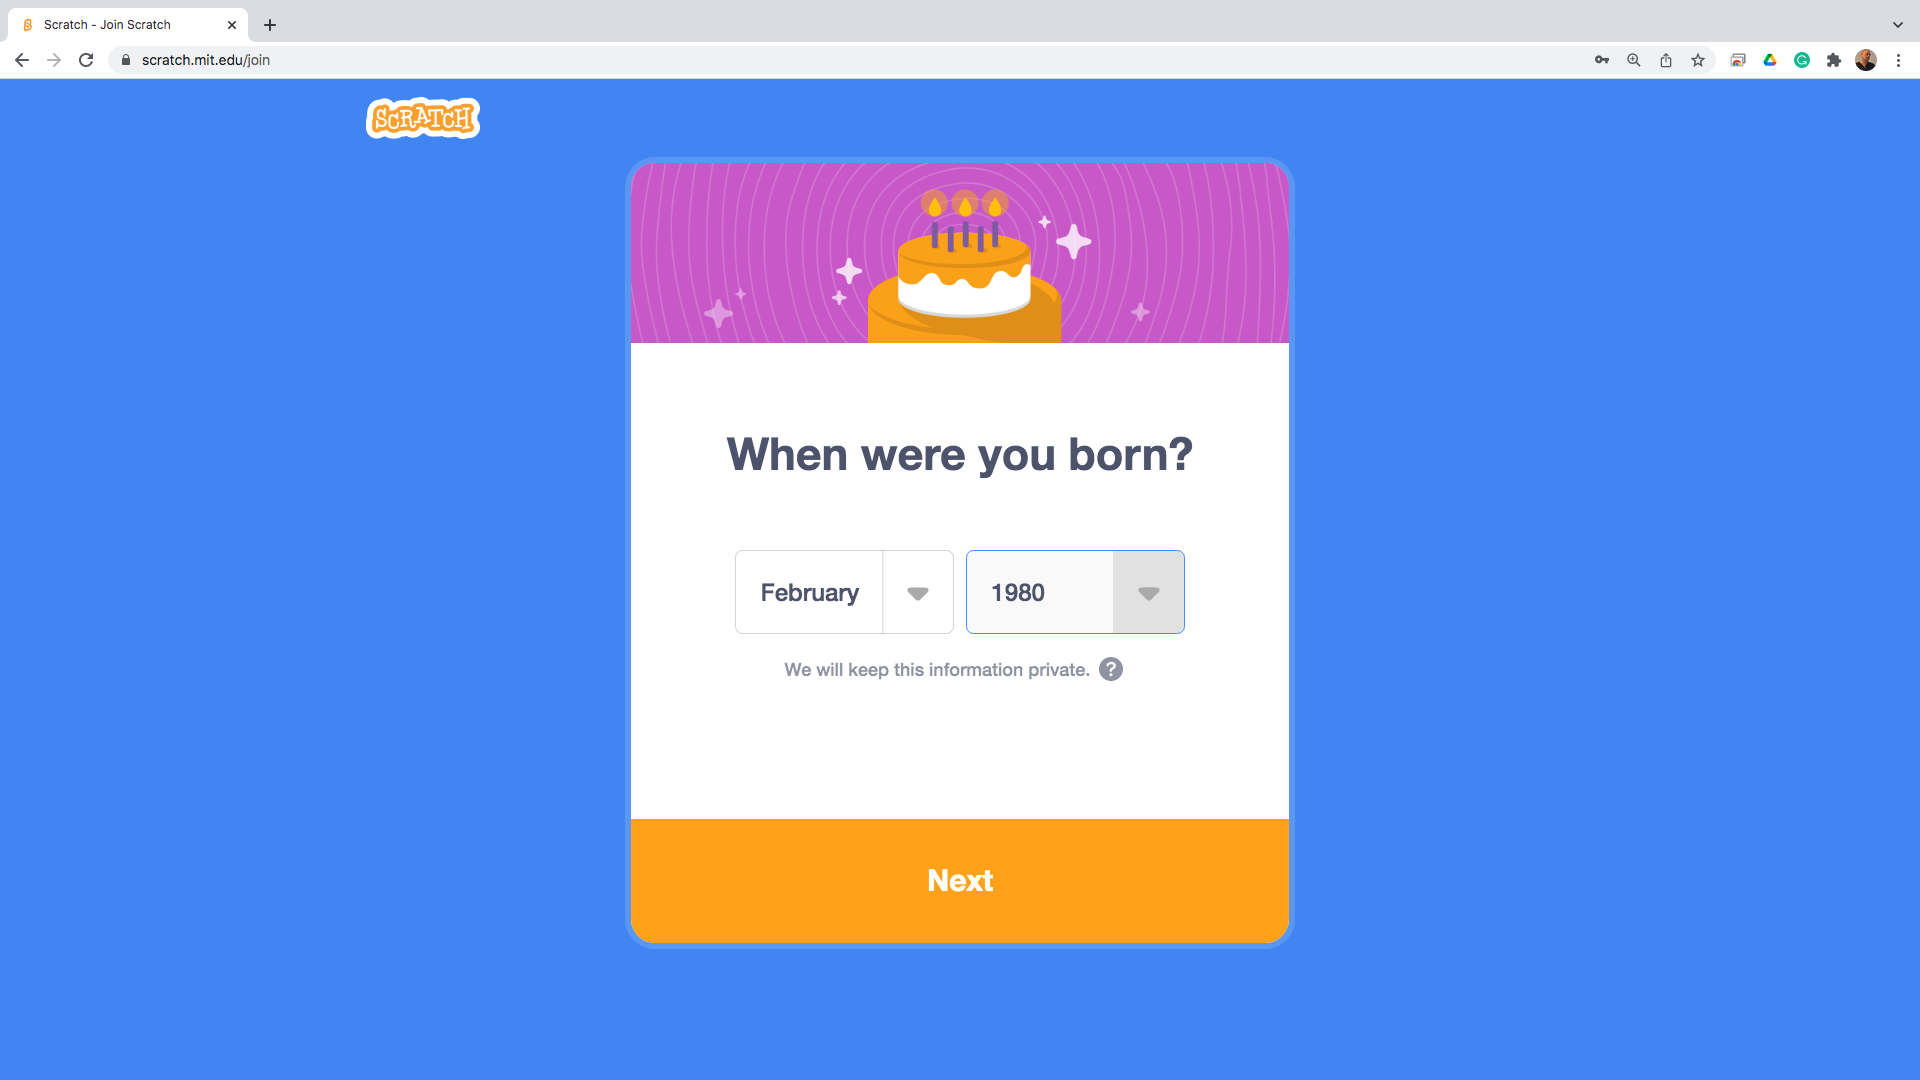
\includegraphics[width=1.0\linewidth,height=0.5\linewidth]{fig010004.png}
   \caption{Age of user}
\label{fig010004}
\end{figure}

In addition to classification by age, the system also collects information on type by gender. This information is optional to avoid discrimination (Fig. \ref{fig010005}).

\begin{figure}[H]
   \centering
   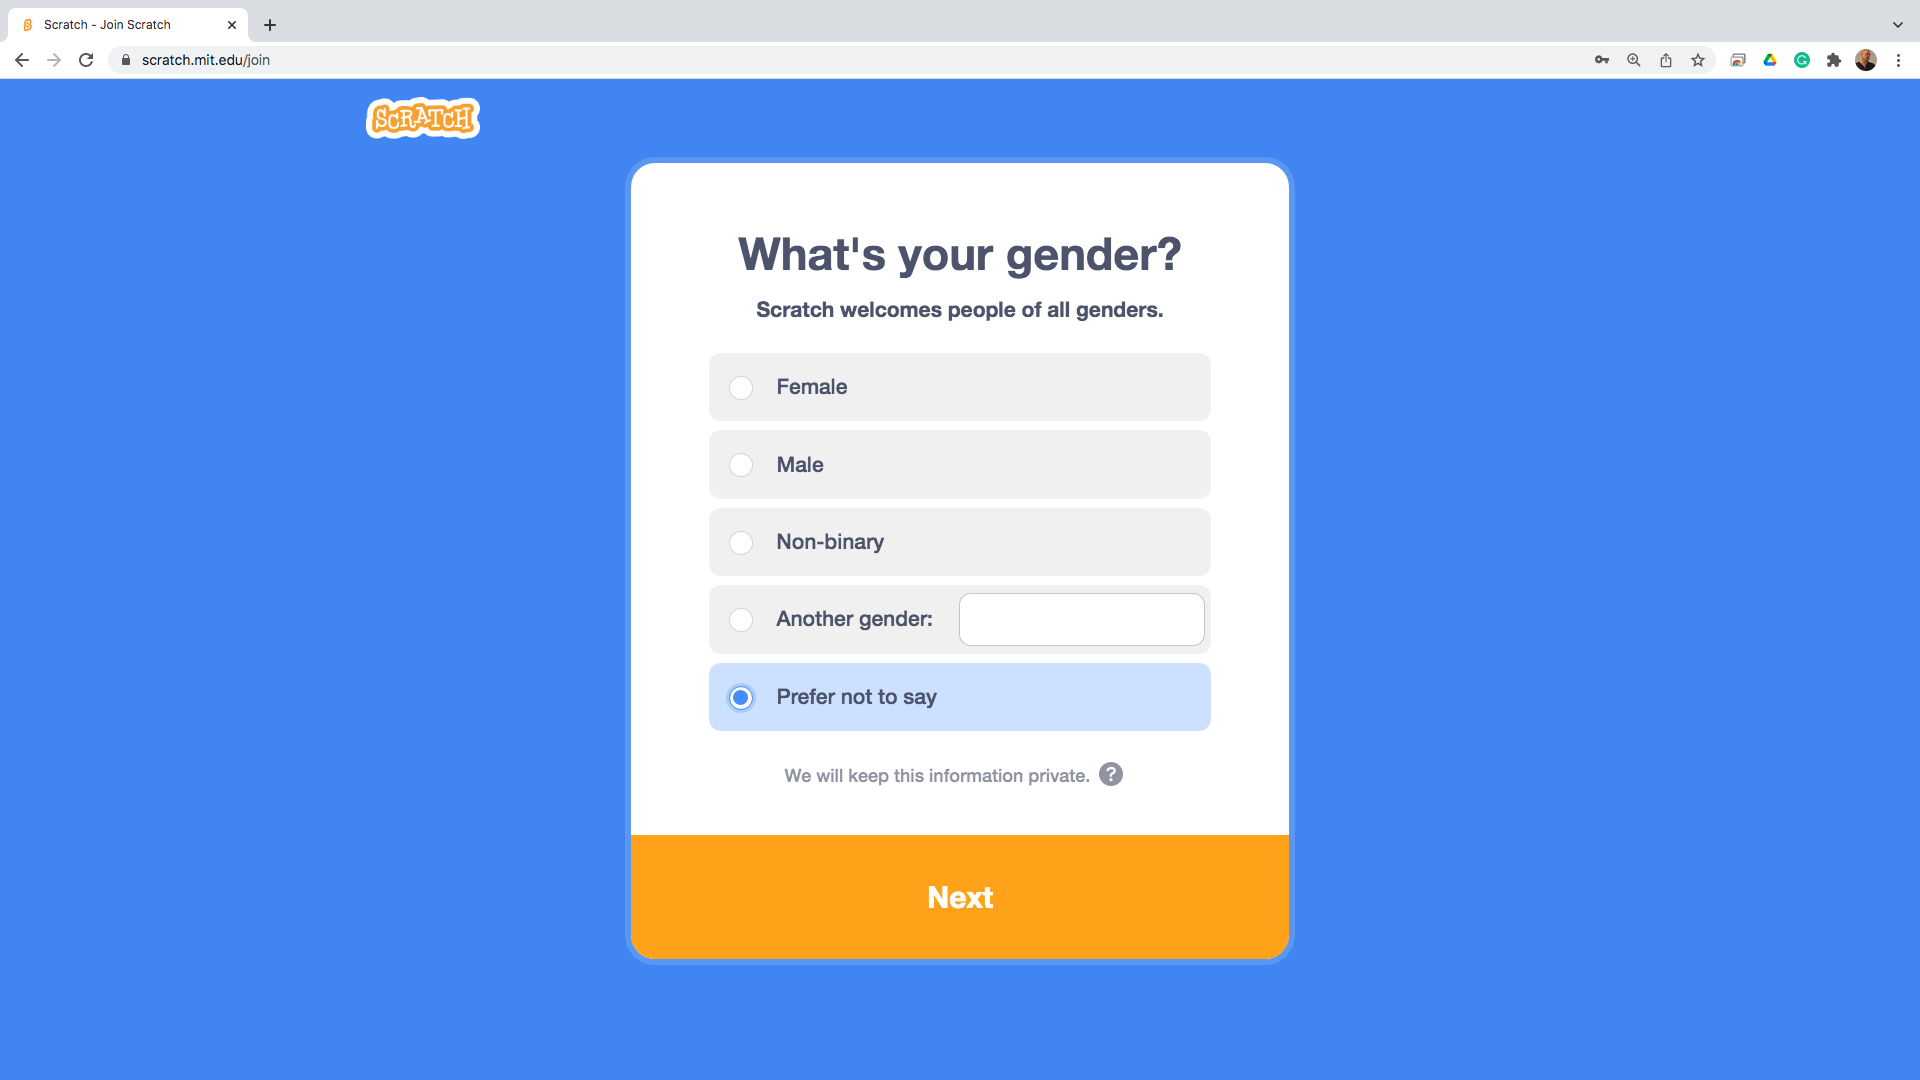
\includegraphics[width=1.0\linewidth,height=0.5\linewidth]{fig010005.png}
   \caption{User gender}
\label{fig010005}
\end{figure}

The user profile, username, and password must also be associated with an email address (Fig. \ref{fig010006}).

\begin{figure}[H]
   \centering
   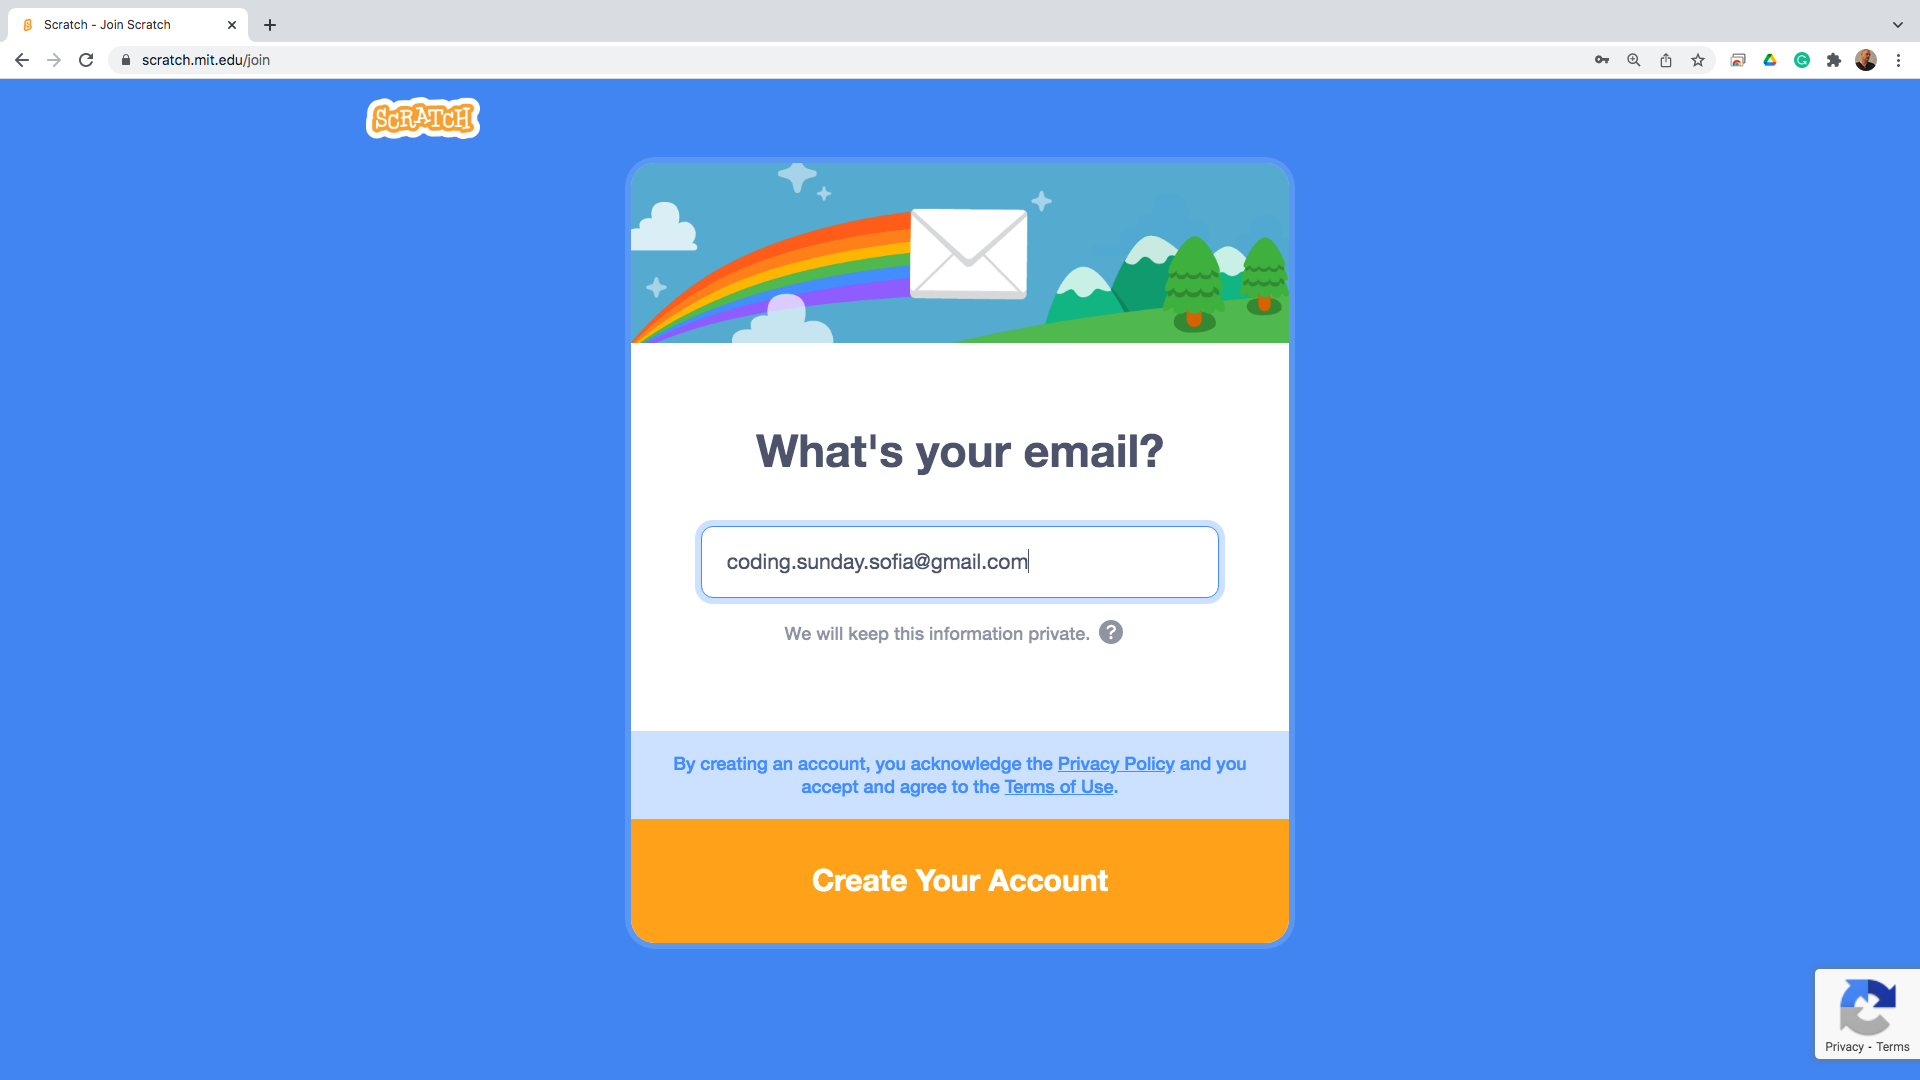
\includegraphics[width=1.0\linewidth,height=0.5\linewidth]{fig010006.png}
   \caption{User email address}
\label{fig010006}
\end{figure}

The system's user registration process is almost complete (Fig. \ref{fig010007}). All that remains is the step to confirm the selected e-mail address.

\begin{figure}[H]
   \centering
   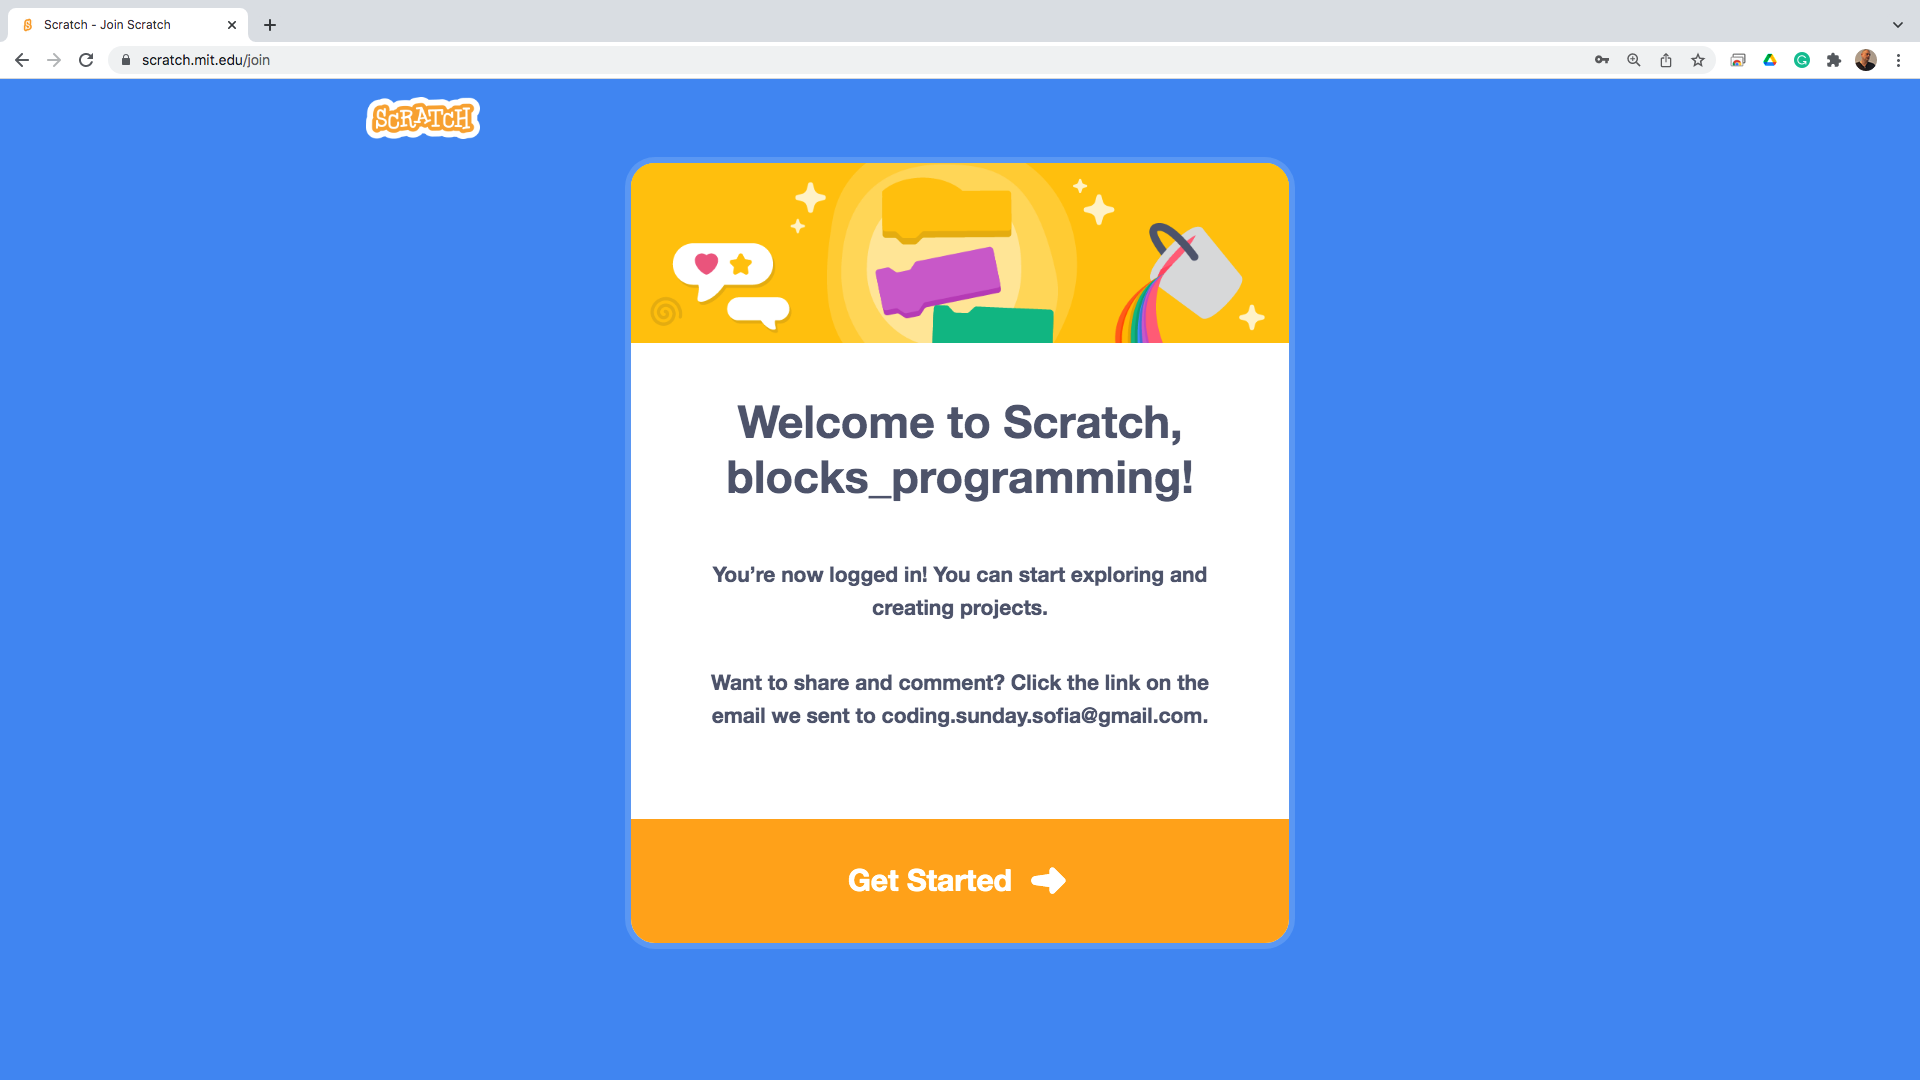
\includegraphics[width=1.0\linewidth,height=0.5\linewidth]{fig010007.png}
   \caption{Completing the user information entry process}
\label{fig010007}
\end{figure}

The email to confirm user registration contains an electronic link to the Scratch website (Fig. \ref{fig010008}). This link must be followed to complete the new user registration process.

\begin{figure}[H]
   \centering
   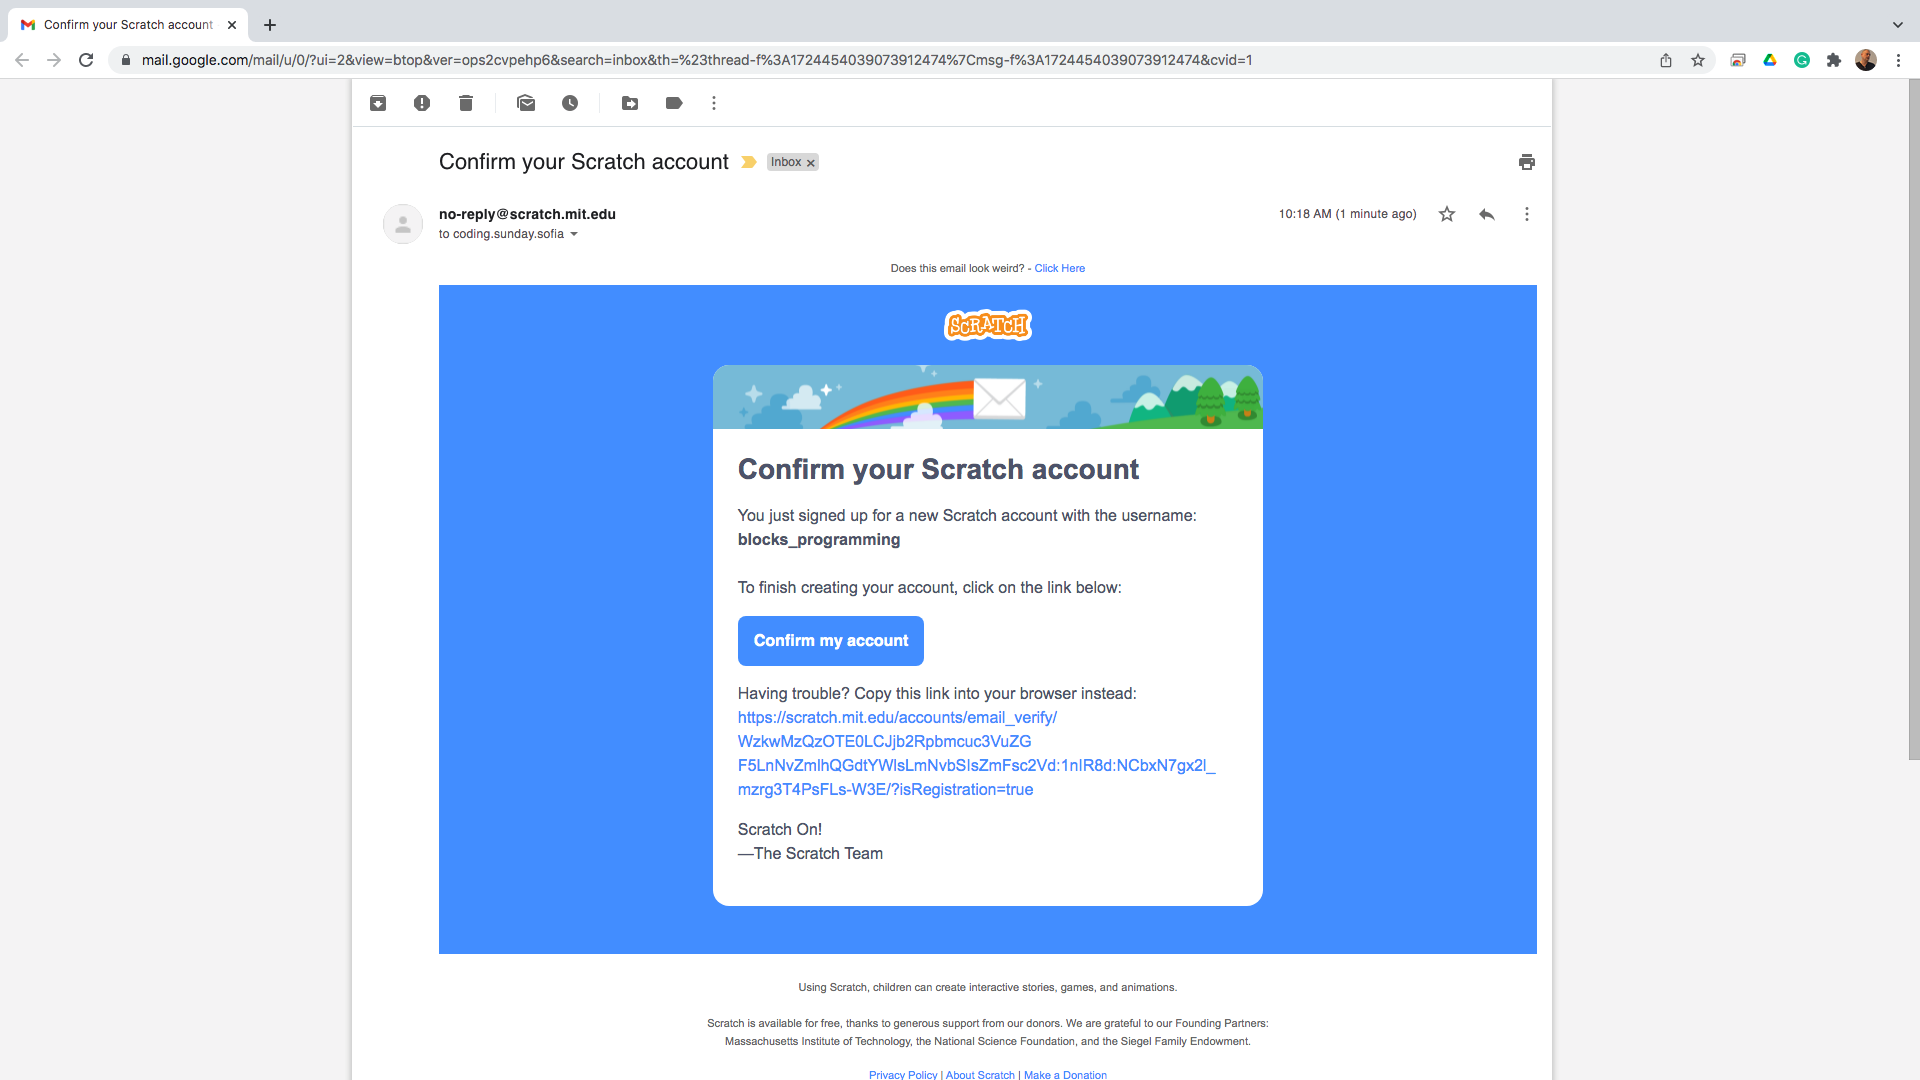
\includegraphics[width=1.0\linewidth,height=0.5\linewidth]{fig010008.png}
   \caption{Email confirmation email}
\label{fig010008}
\end{figure}

The registration of the new user ends with loading the initial working screen (Fig. \ref{fig010009}). At the top right, you can see the username chosen in the first step of the registration process.

\begin{figure}[H]
   \centering
   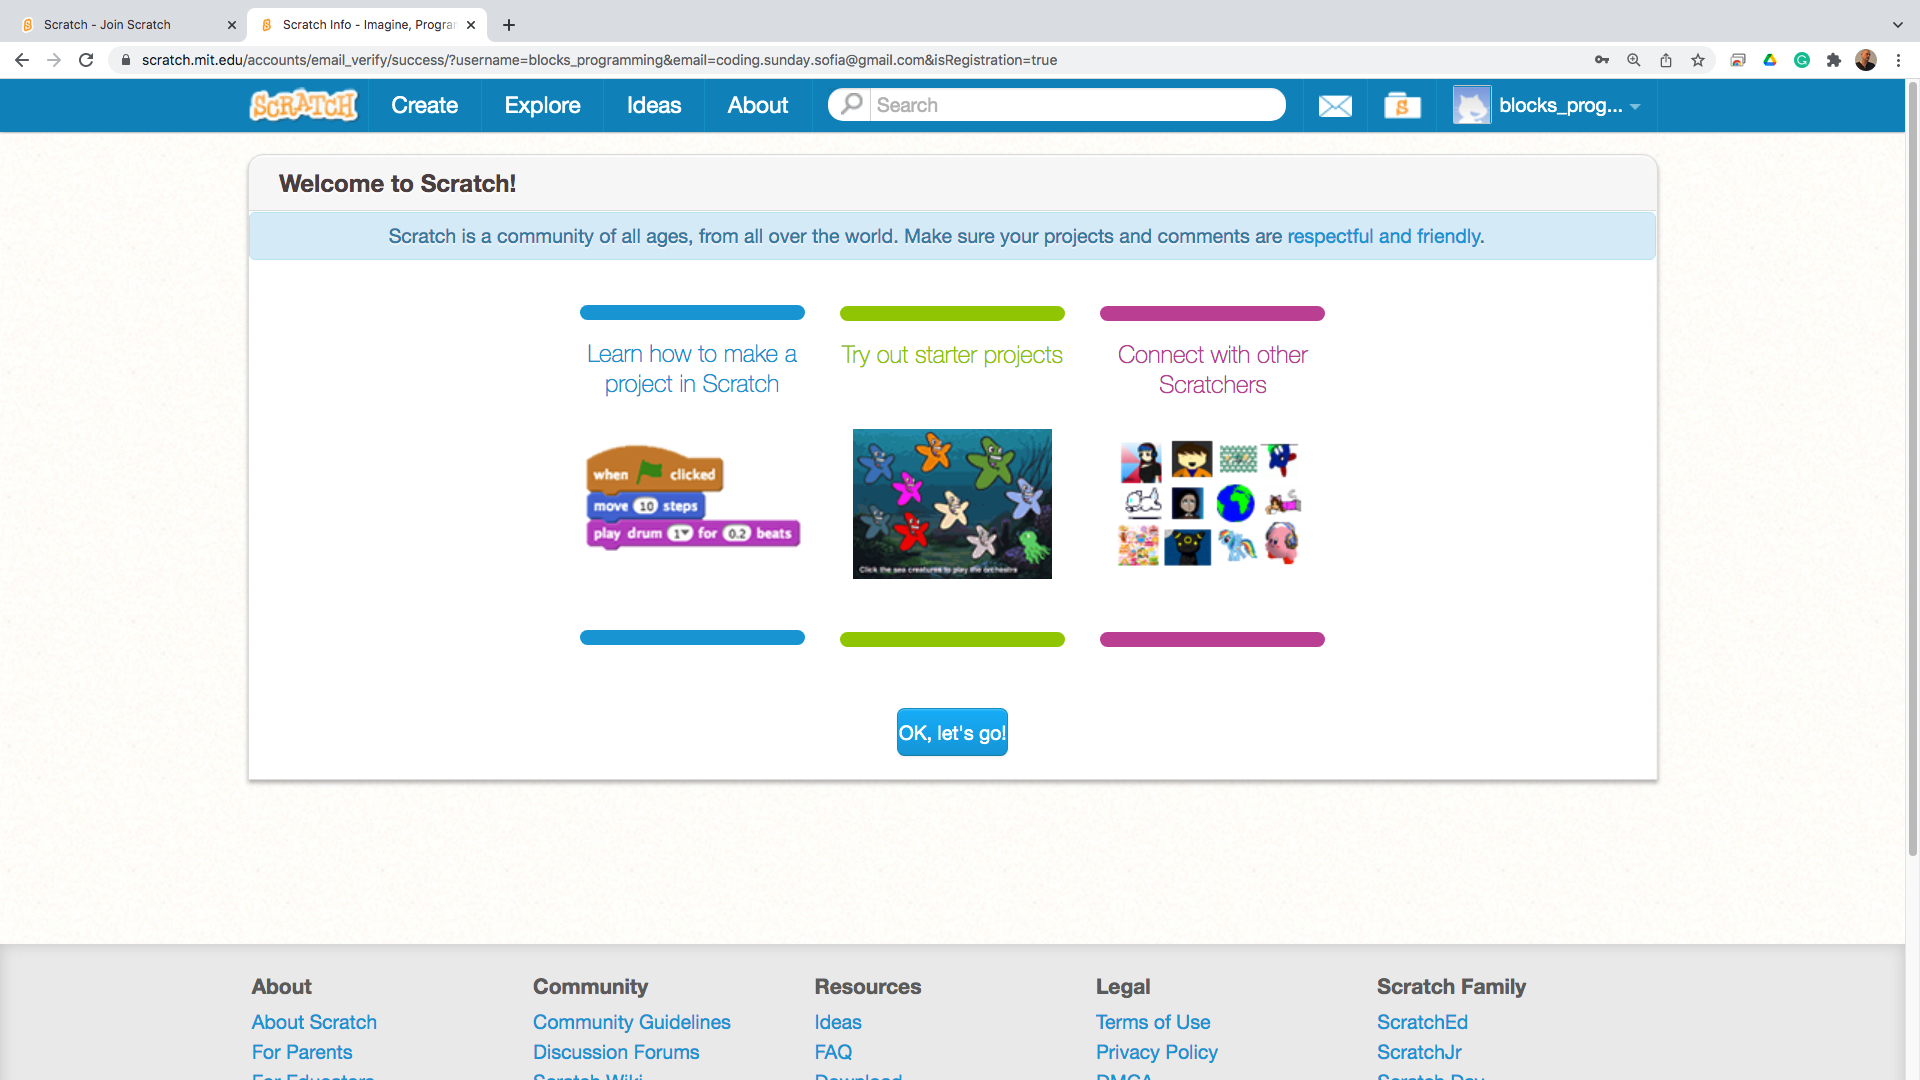
\includegraphics[width=1.0\linewidth,height=0.5\linewidth]{fig010009.png}
   \caption{Home screen}
\label{fig010009}
\end{figure}

Creating a small project demonstrating the development environment can also confirm successful registration. For this purpose, the "Create" option is selected from the menu (Fig. \ref{fig010010}).

\begin{figure}[H]
   \centering
   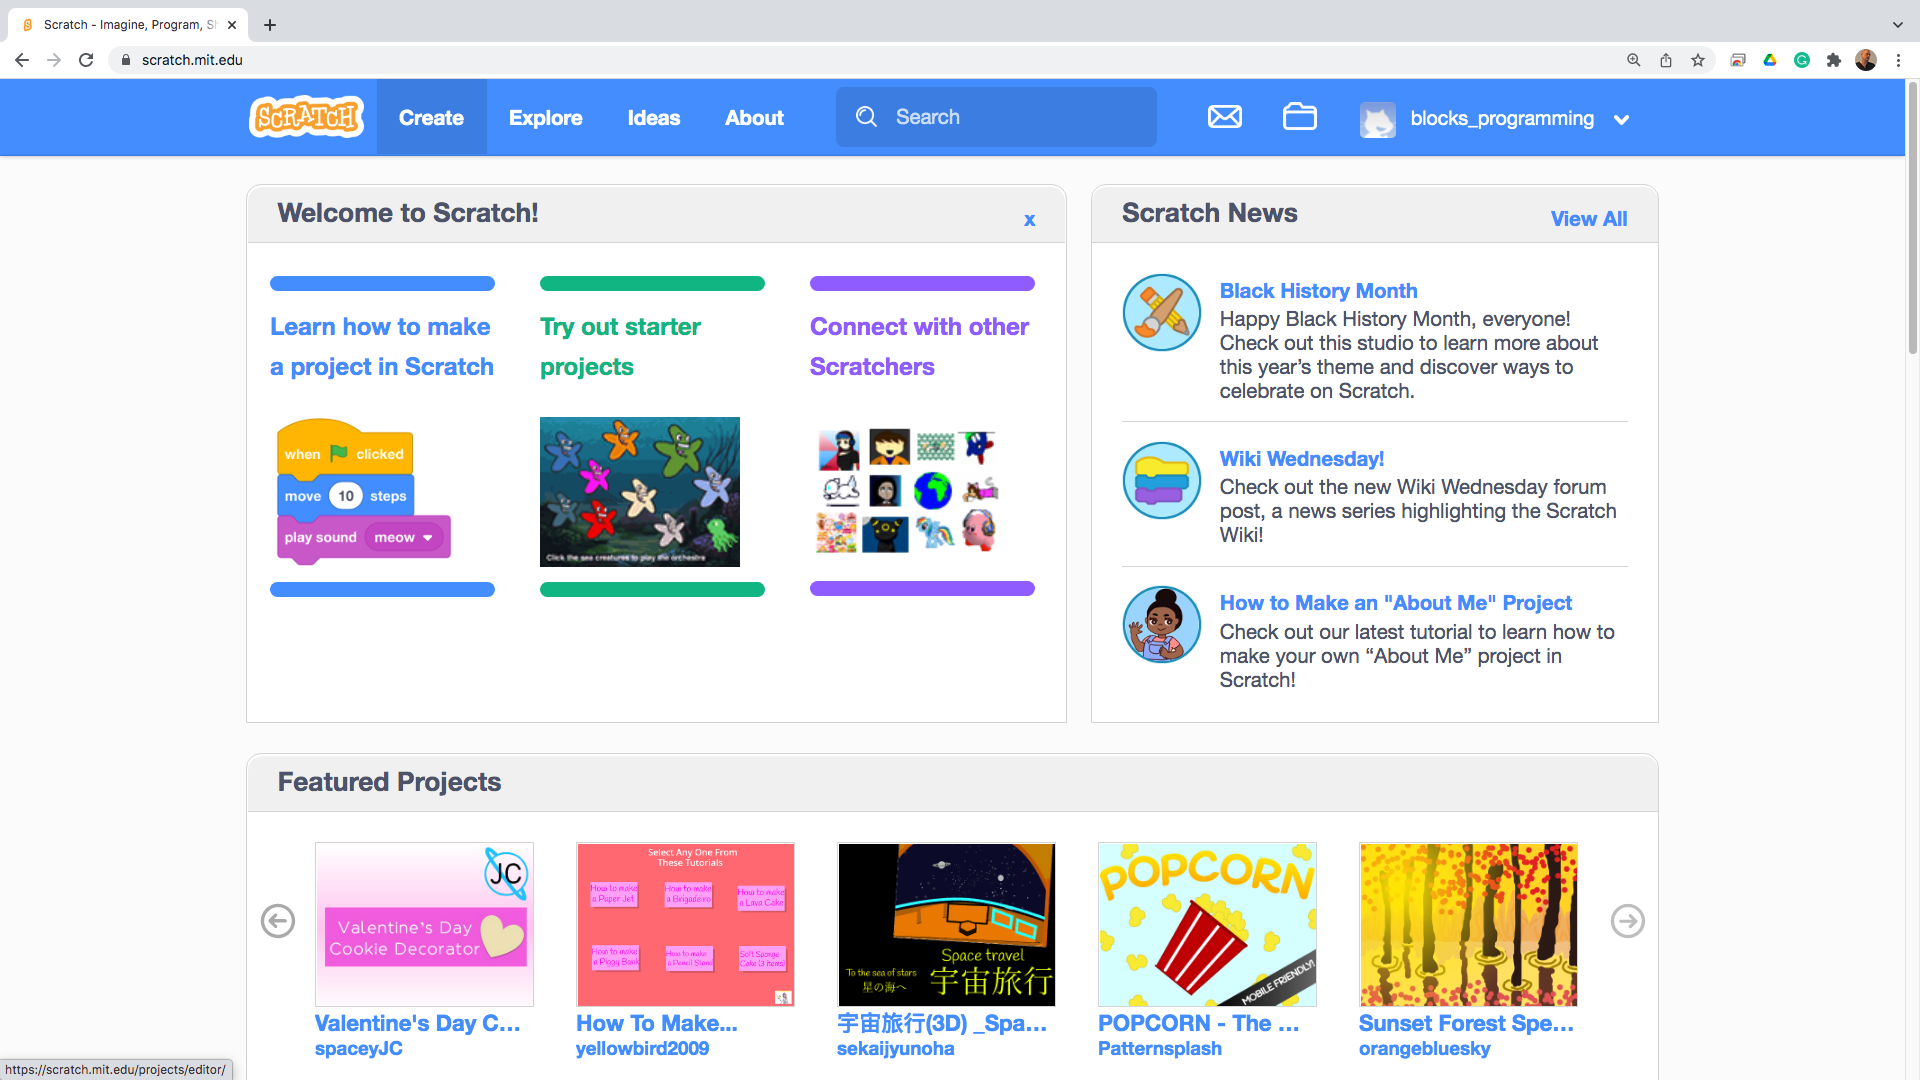
\includegraphics[width=1.0\linewidth,height=0.5\linewidth]{fig010010.png}
   \caption{Selecting a New Project Menu Option}
\label{fig010010}
\end{figure}

Creating a new project goes through a series of steps related to allocating the initially needed resources (Fig. \ref{fig010011}).

\begin{figure}[H]
   \centering
   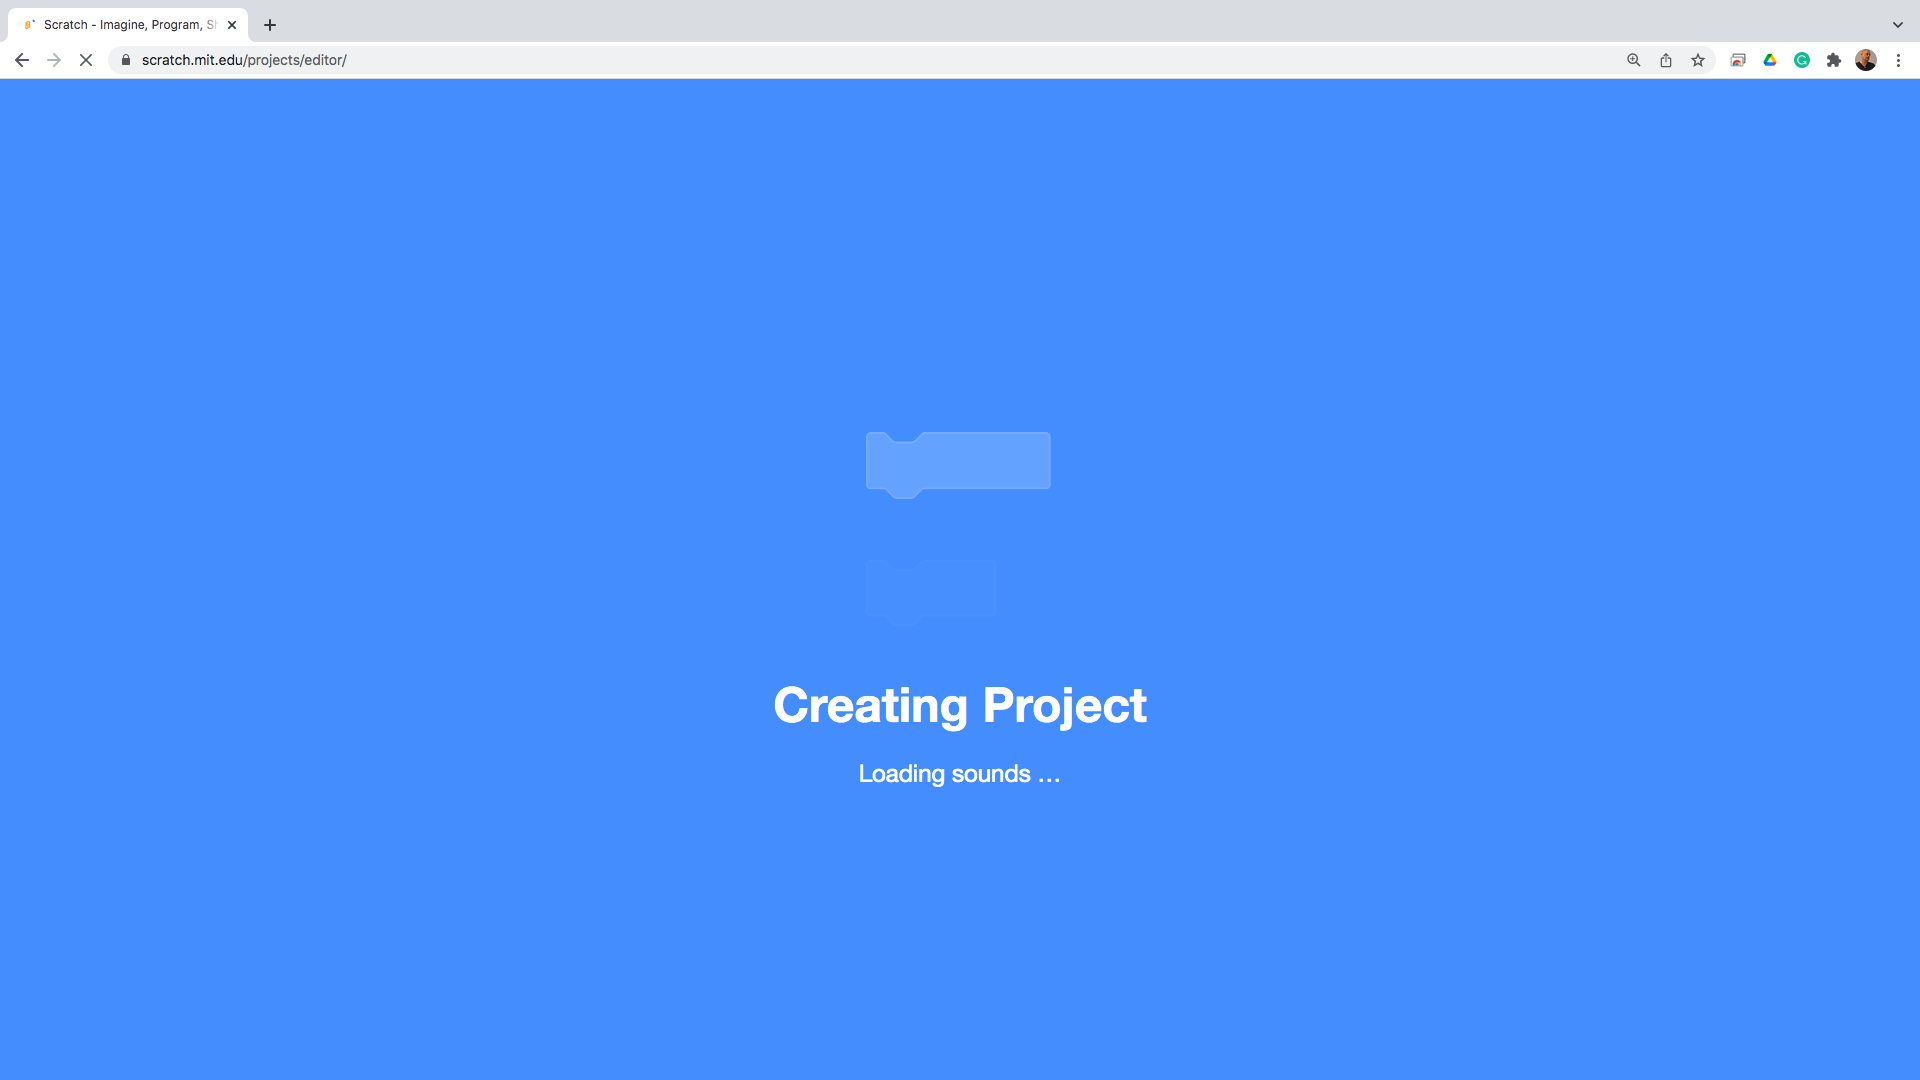
\includegraphics[width=1.0\linewidth,height=0.5\linewidth]{fig010011.png}
   \caption{Loading Resources}
\label{fig010011}
\end{figure}

The workspace is visualized after loading the new project (Fig. \ref{fig010012}). On the far left is the list of possible program instructions in the form of puzzle pieces. In the central part is the workspace where the instructions are arranged. And on the far right is the active stage, where the actions embedded in the instructions are visualized.

\begin{figure}[H]
   \centering
   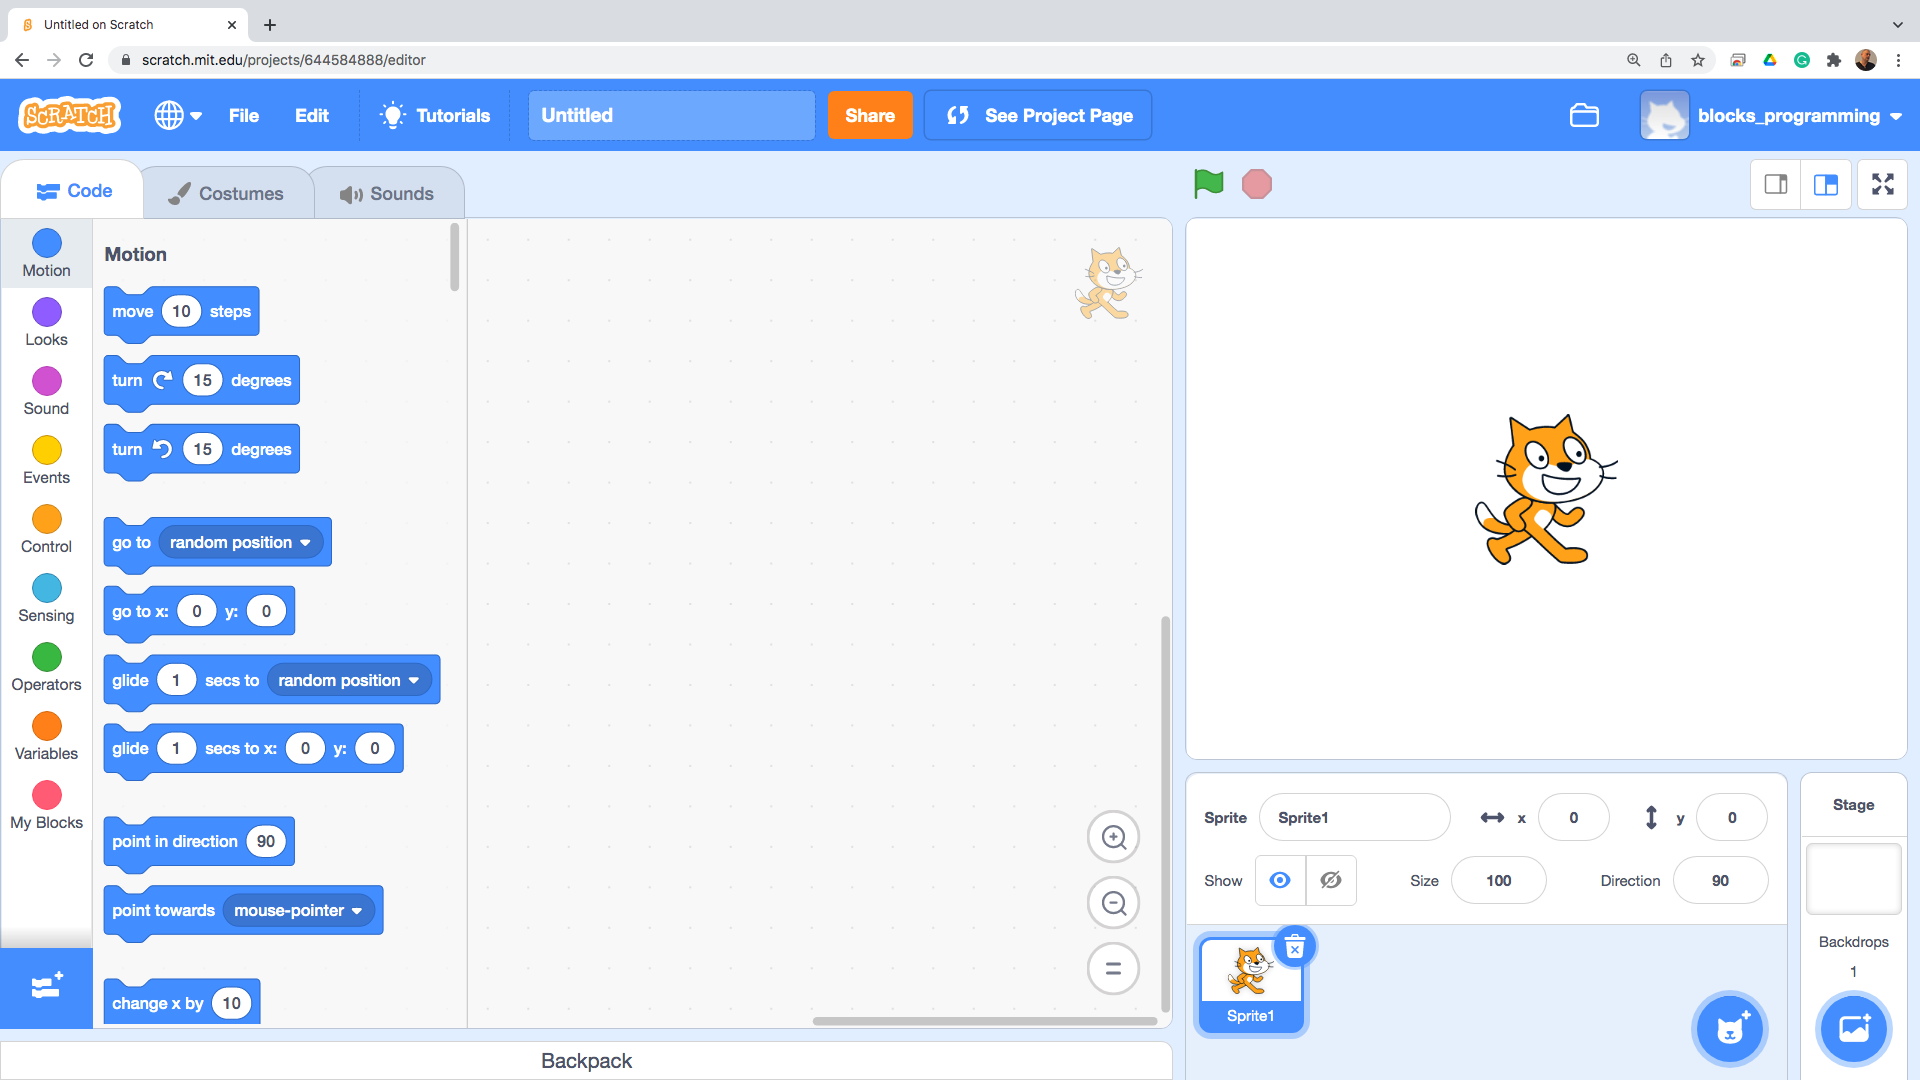
\includegraphics[width=1.0\linewidth,height=0.5\linewidth]{fig010012.png}
   \caption{Workspace Organization}
\label{fig010012}
\end{figure}

Every computer program has its starting point and its ending point. In Scratch, there is a particular block (program instruction) for the beginning of the program, which is shown in Fig. \ref{fig010013}. The execution of the programs written in Scratch starts when the green flag is pressed. Therefore, the program launch block is bound to the green flag click event.

\begin{figure}[H]
   \centering
   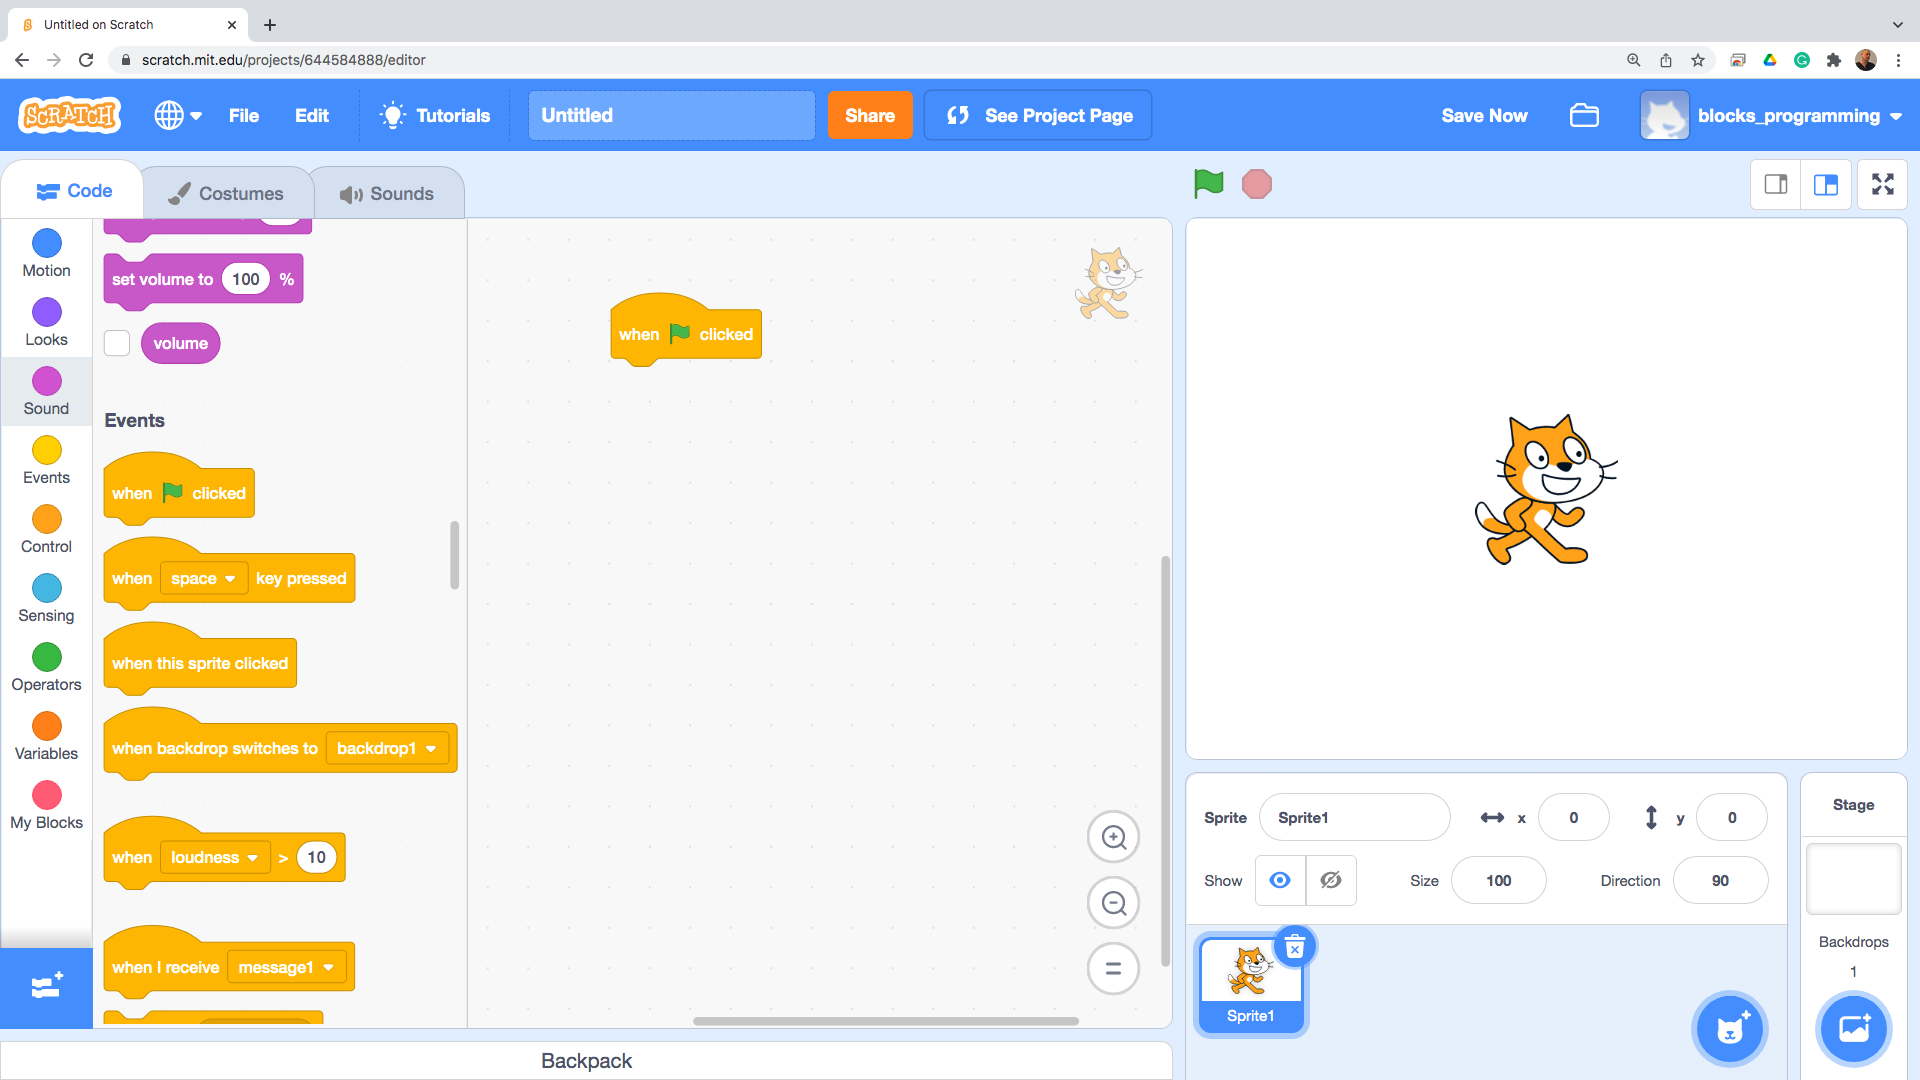
\includegraphics[width=1.0\linewidth,height=0.5\linewidth]{fig010013.png}
   \caption{Start of program}
\label{fig010013}
\end{figure}

One of the most intuitive and, simultaneously, easy-to-understand instructions is to move by a certain number of steps (Fig. \ref{fig010014}). The main actor in the opening scene of Scratch is the orange cat. If the scene is not changed, the instructions to perform various actions are directed directly to that cat.

\begin{figure}[H]
   \centering
   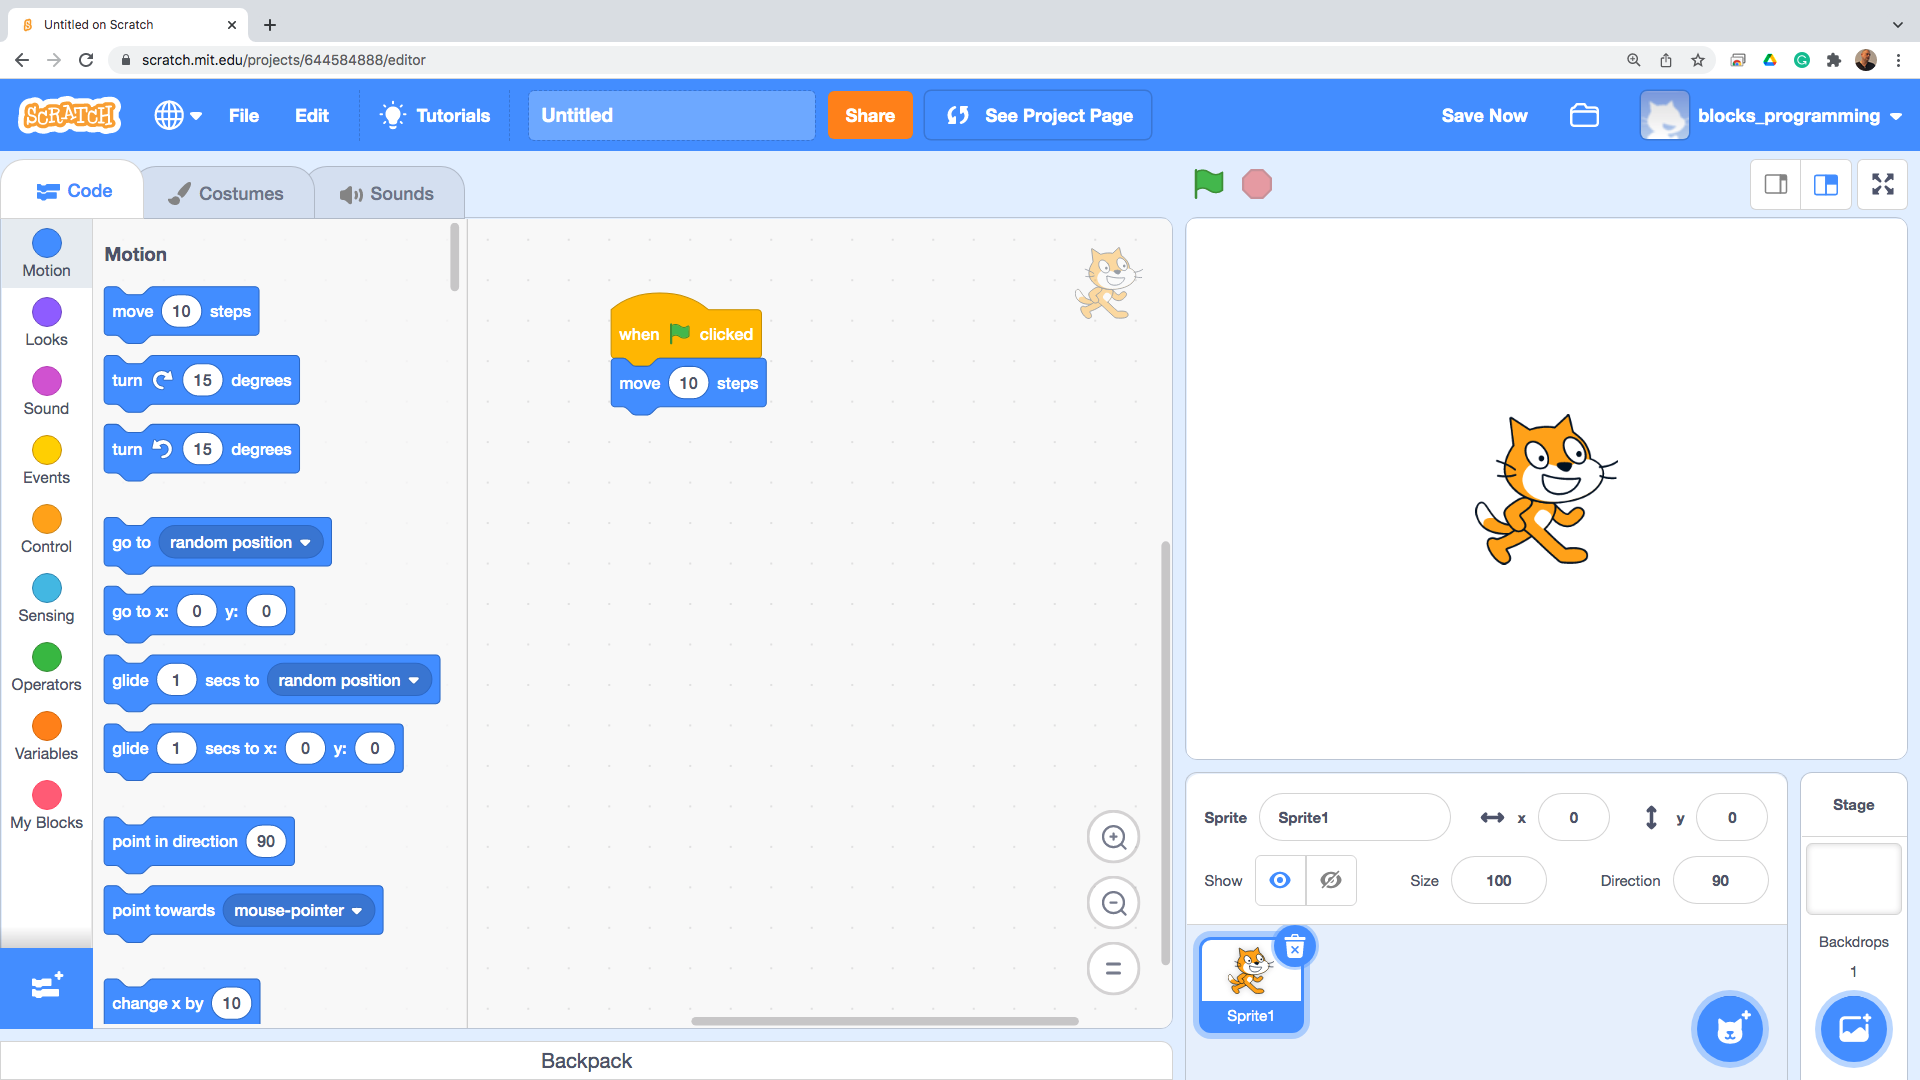
\includegraphics[width=1.0\linewidth,height=0.5\linewidth]{fig010014.png}
   \caption{Step-by-step instructions}
\label{fig010014}
\end{figure}

After the cat is moved, there must be a waiting pause so that the move is visually noted. For this purpose, a wait instruction can be implemented for a certain number of seconds (Fig. \ref{fig010015}).

\begin{figure}[H]
   \centering
   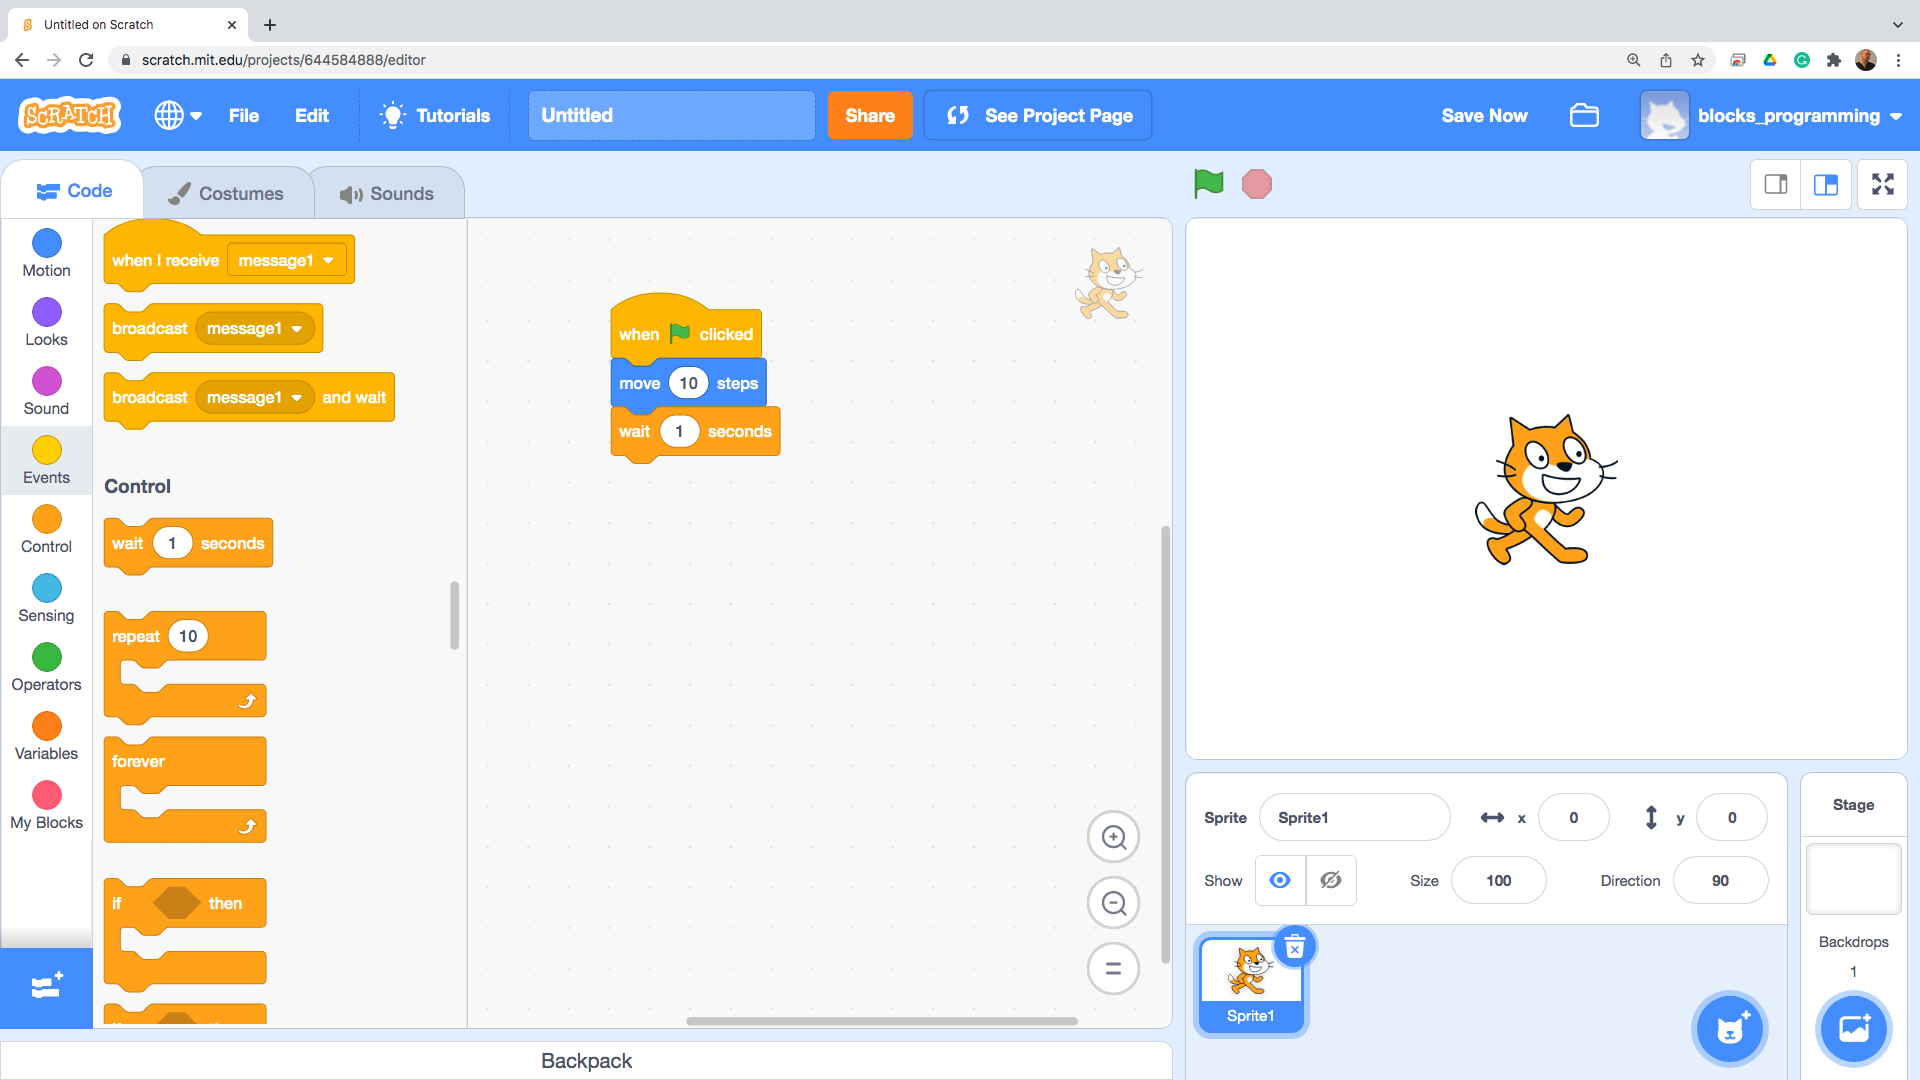
\includegraphics[width=1.0\linewidth,height=0.5\linewidth]{fig010015.png}
   \caption{Wait instruction}
\label{fig010015}
\end{figure}

After the wait, the cat can return to its original position by executing a move instruction with a negative number of steps (Fig. \ref{fig010016}).

\begin{figure}[H]
   \centering
   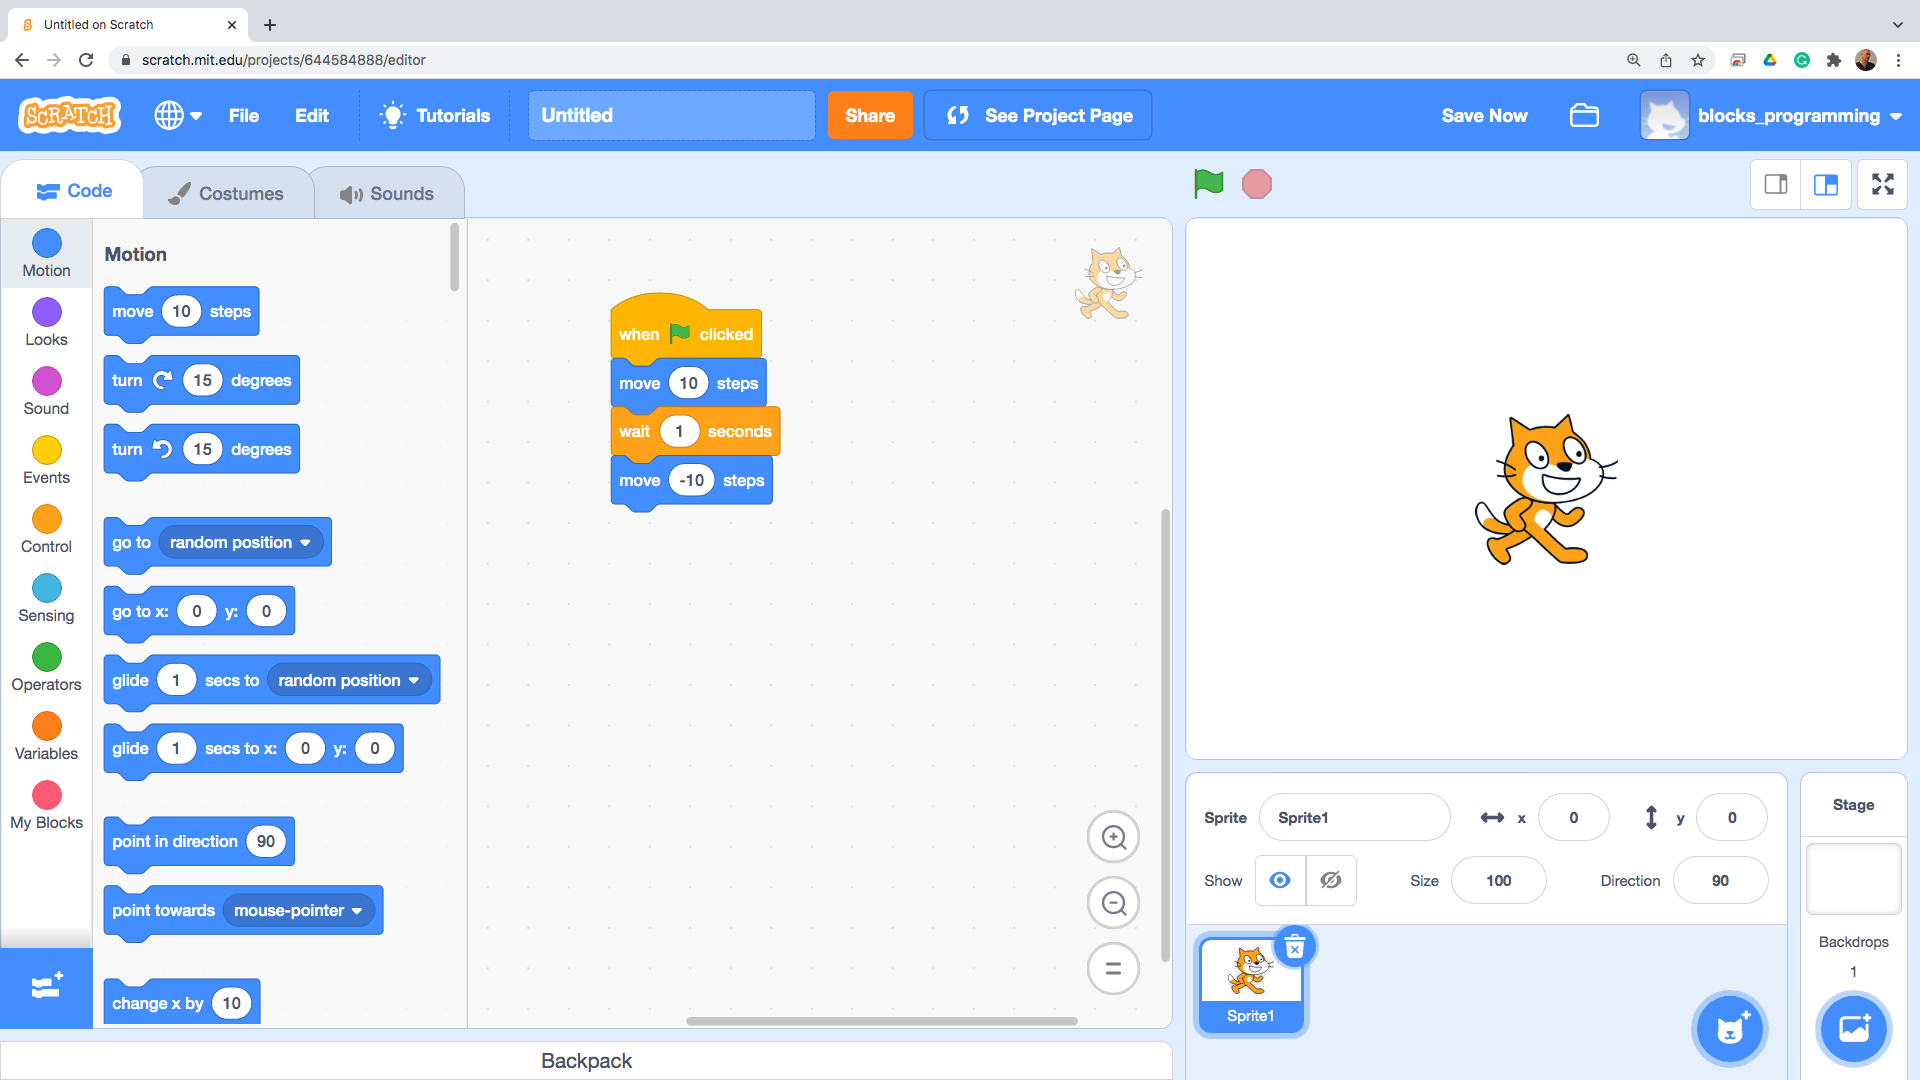
\includegraphics[width=1.0\linewidth,height=0.5\linewidth]{fig010016.png}
   \caption{Instructions for moving back}
\label{fig010016}
\end{figure}

After all the intended instructions have been executed, it is reasonable to end the program, for which a separate block is provided in the list of instructions (Fig. \ref{fig010017}).

\begin{figure}[H]
   \centering
   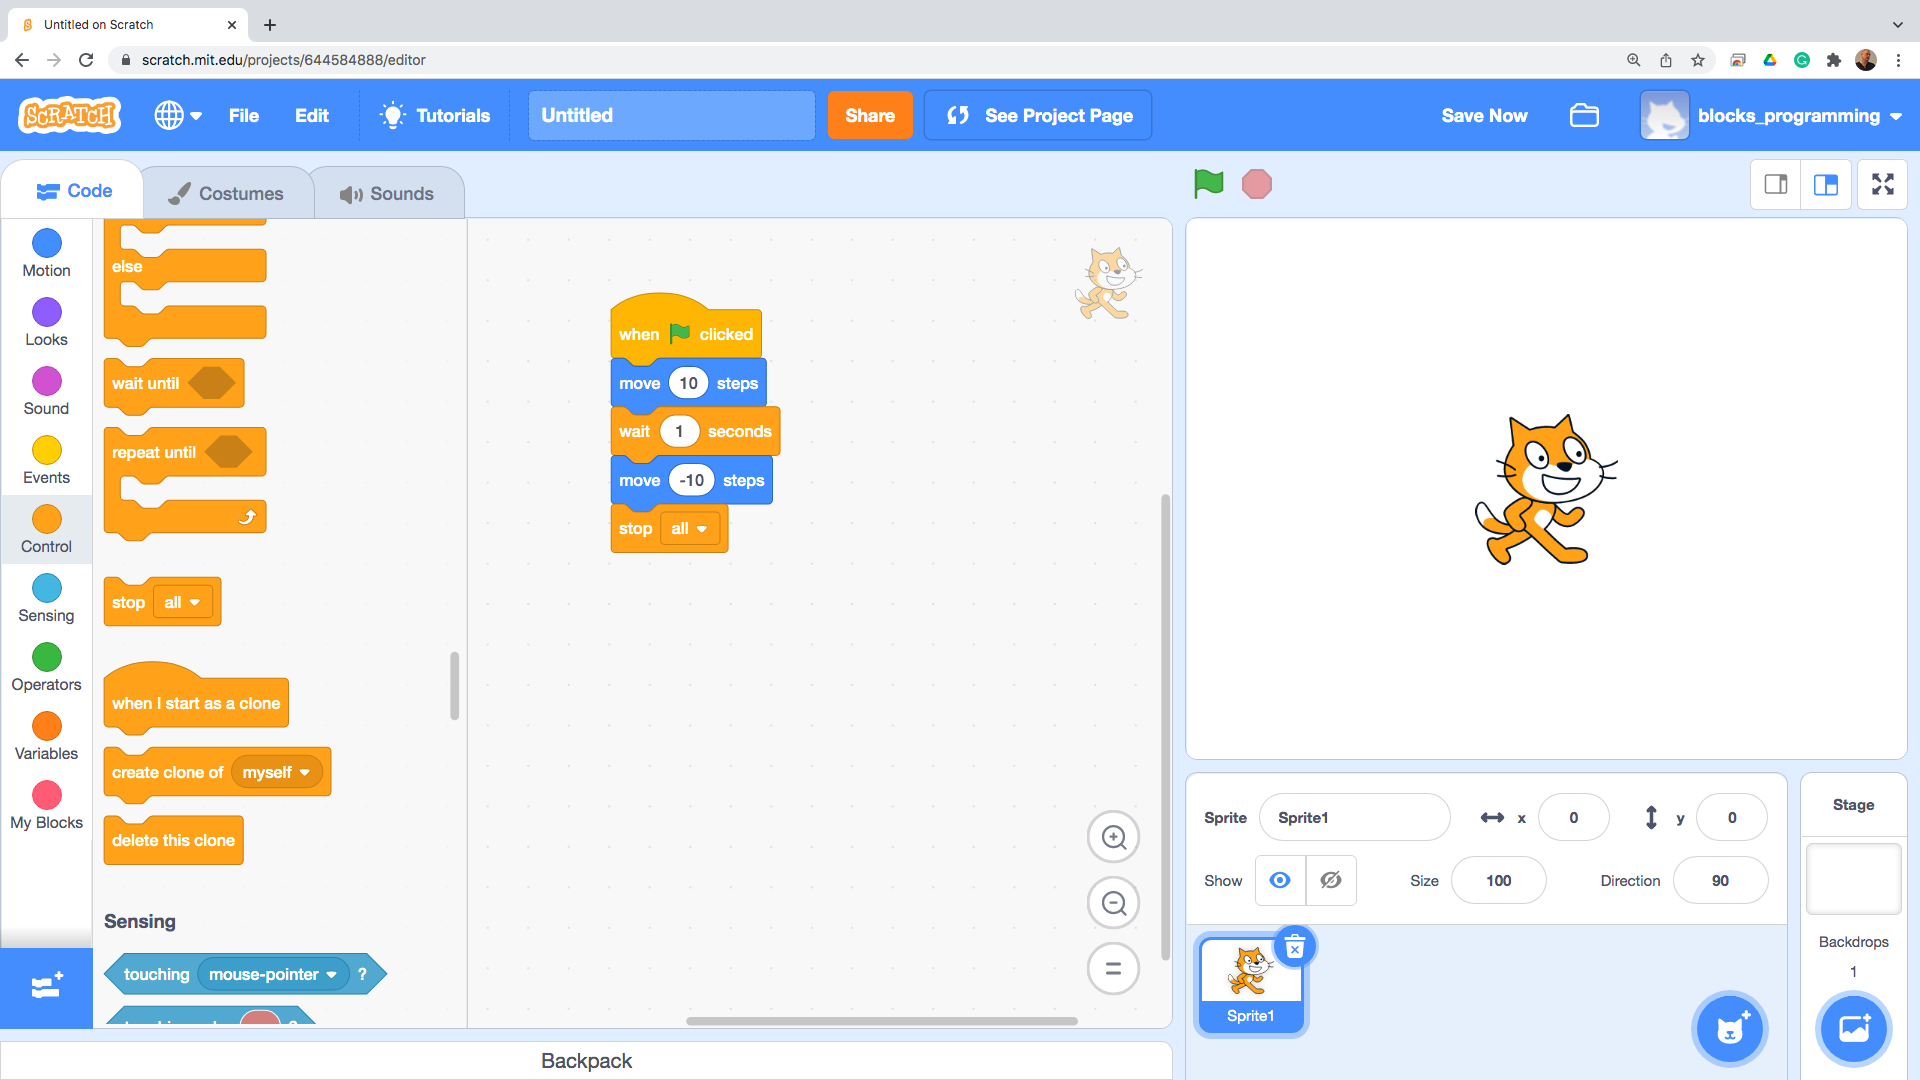
\includegraphics[width=1.0\linewidth,height=0.5\linewidth]{fig010017.png}
   \caption{End instruction}
\label{fig010017}
\end{figure}

The program written in this way is executed by pressing the green flag (Fig. \ref{fig010018}), and if an emergency stop is needed, press the red circle to the right of the green flag.

\begin{figure}[H]
   \centering
   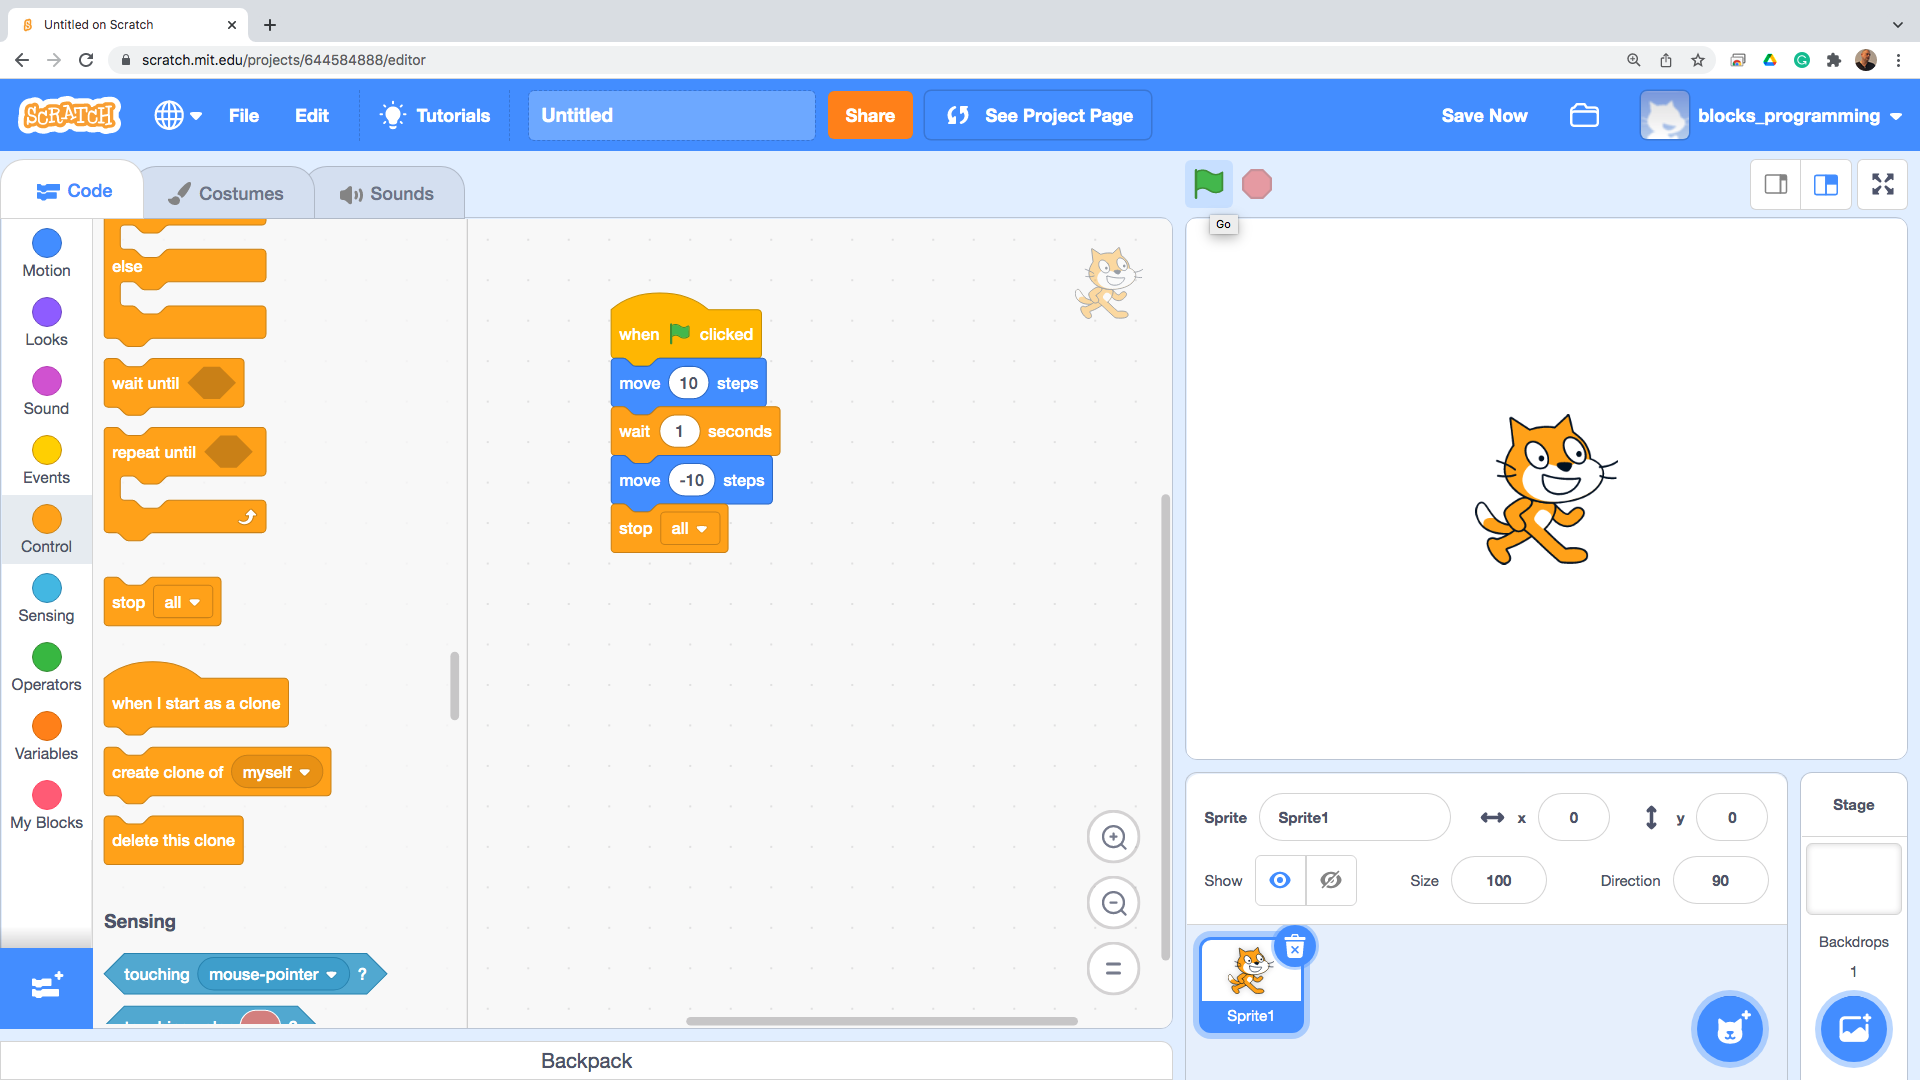
\includegraphics[width=1.0\linewidth,height=0.5\linewidth]{fig010018.png}
   \caption{Program Execution}
\label{fig010018}
\end{figure}

Each program that is written in Scratch is placed in a separate project. All of the user's projects can be accessed from the "My Stuff" menu, which is part of the list of options for handling the registered user (Fig. \ref{fig010019}).

\begin{figure}[H]
   \centering
   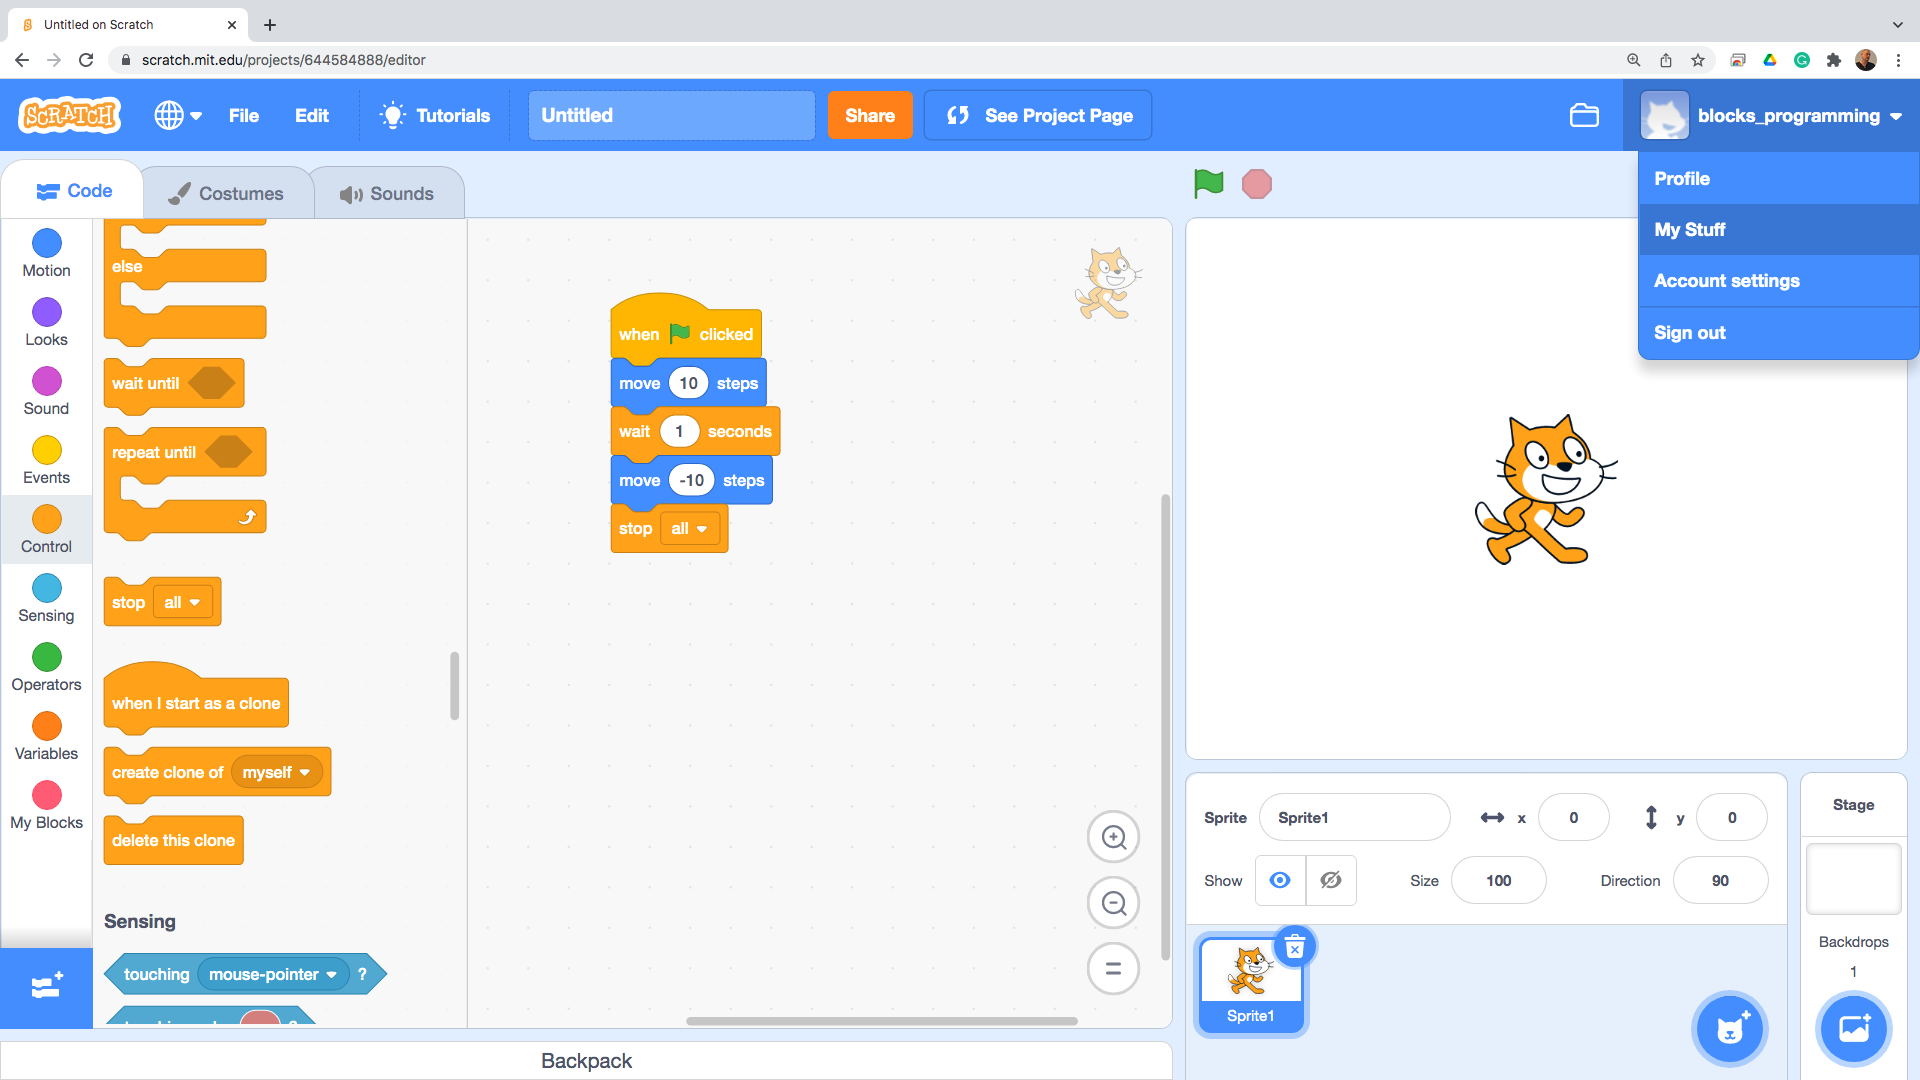
\includegraphics[width=1.0\linewidth,height=0.5\linewidth]{fig010019.png}
   \caption{Project Organization Menu}
\label{fig010019}
\end{figure}

Initially, each project has a working name (Fig. \ref{fig010020}), which can be changed later. One of the most attractive advantages of the programming environment is that users' projects can be shared (Sharing) with a vast audience. This allows a quick transfer of knowledge and skills and an assessment of the work done.

\begin{figure}[H]
   \centering
   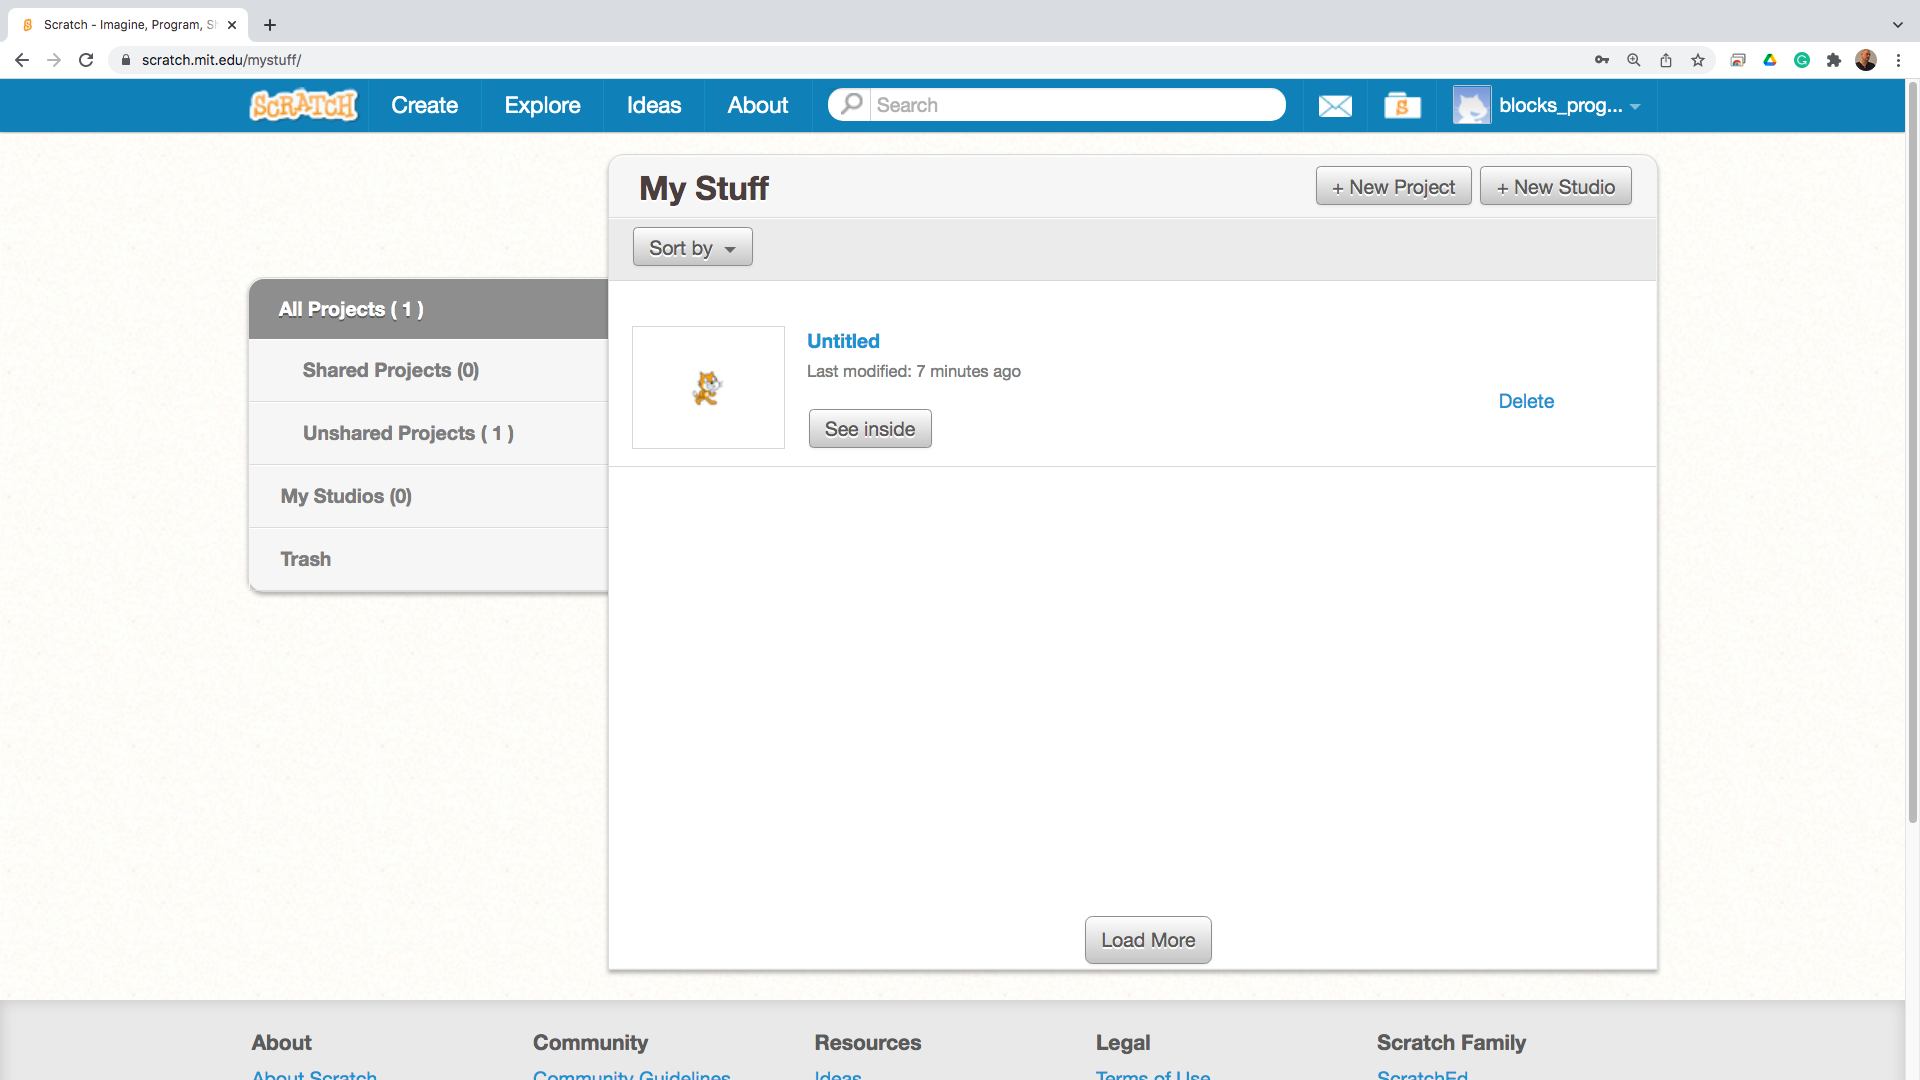
\includegraphics[width=1.0\linewidth,height=0.5\linewidth]{fig010020.png}
   \caption{List of projects}
\label{fig010020}
\end{figure}

The greatest fascination with block languages comes from writing the instructions and forming a complete program, like putting together a puzzle. Almost all children like to put together puzzles. They like bright colors and beautiful pictures. When the charm of classic puzzles is transferred to a field as attractive as programming, the results can be astounding.

\section{Getting Started in App Inventor}

Working in the App Inventor environment begins by loading the main web page (Fig. \ref{fig010021}), which is located at: \\ \href{https://appinventor.mit.edu/}{https:// appinventor.mit.edu/}

\begin{figure}[H]
   \centering
   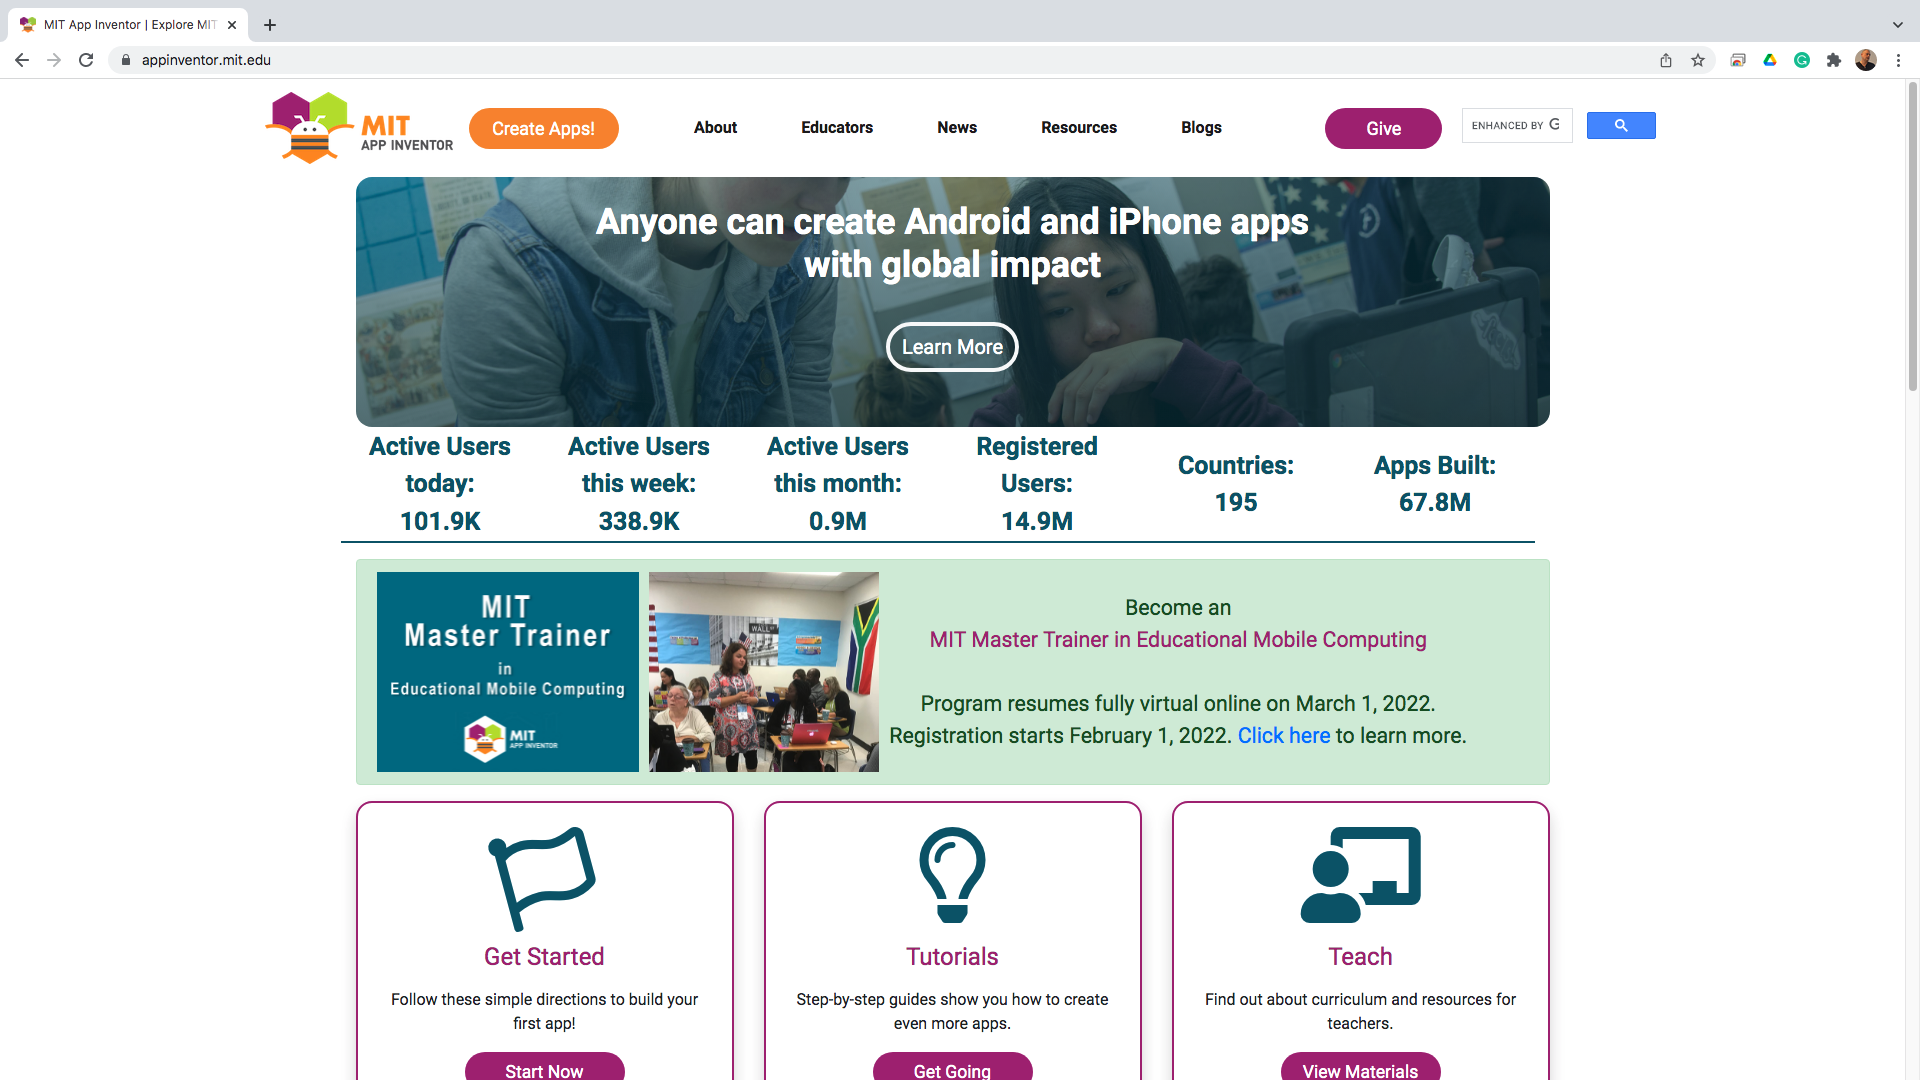
\includegraphics[width=1.0\linewidth,height=0.5\linewidth]{fig010021.png}
   \caption{App Inventor Home Web Page}
\label{fig010021}
\end{figure}

Although App Inventor is also a product of the Massachusetts Institute of Technology, working with it in some aspects differs from how you work in Scratch. App Inventor is also available as a cloud service where registration is required. Unlike Scratch, in App Inventor, you can skip creating a user profile and log in to the system through classic registration in the GMail service. This process starts after selecting the orange "Create Apps!" button (Fig. \ref{fig010022}).

\begin{figure}[H]
   \centering
   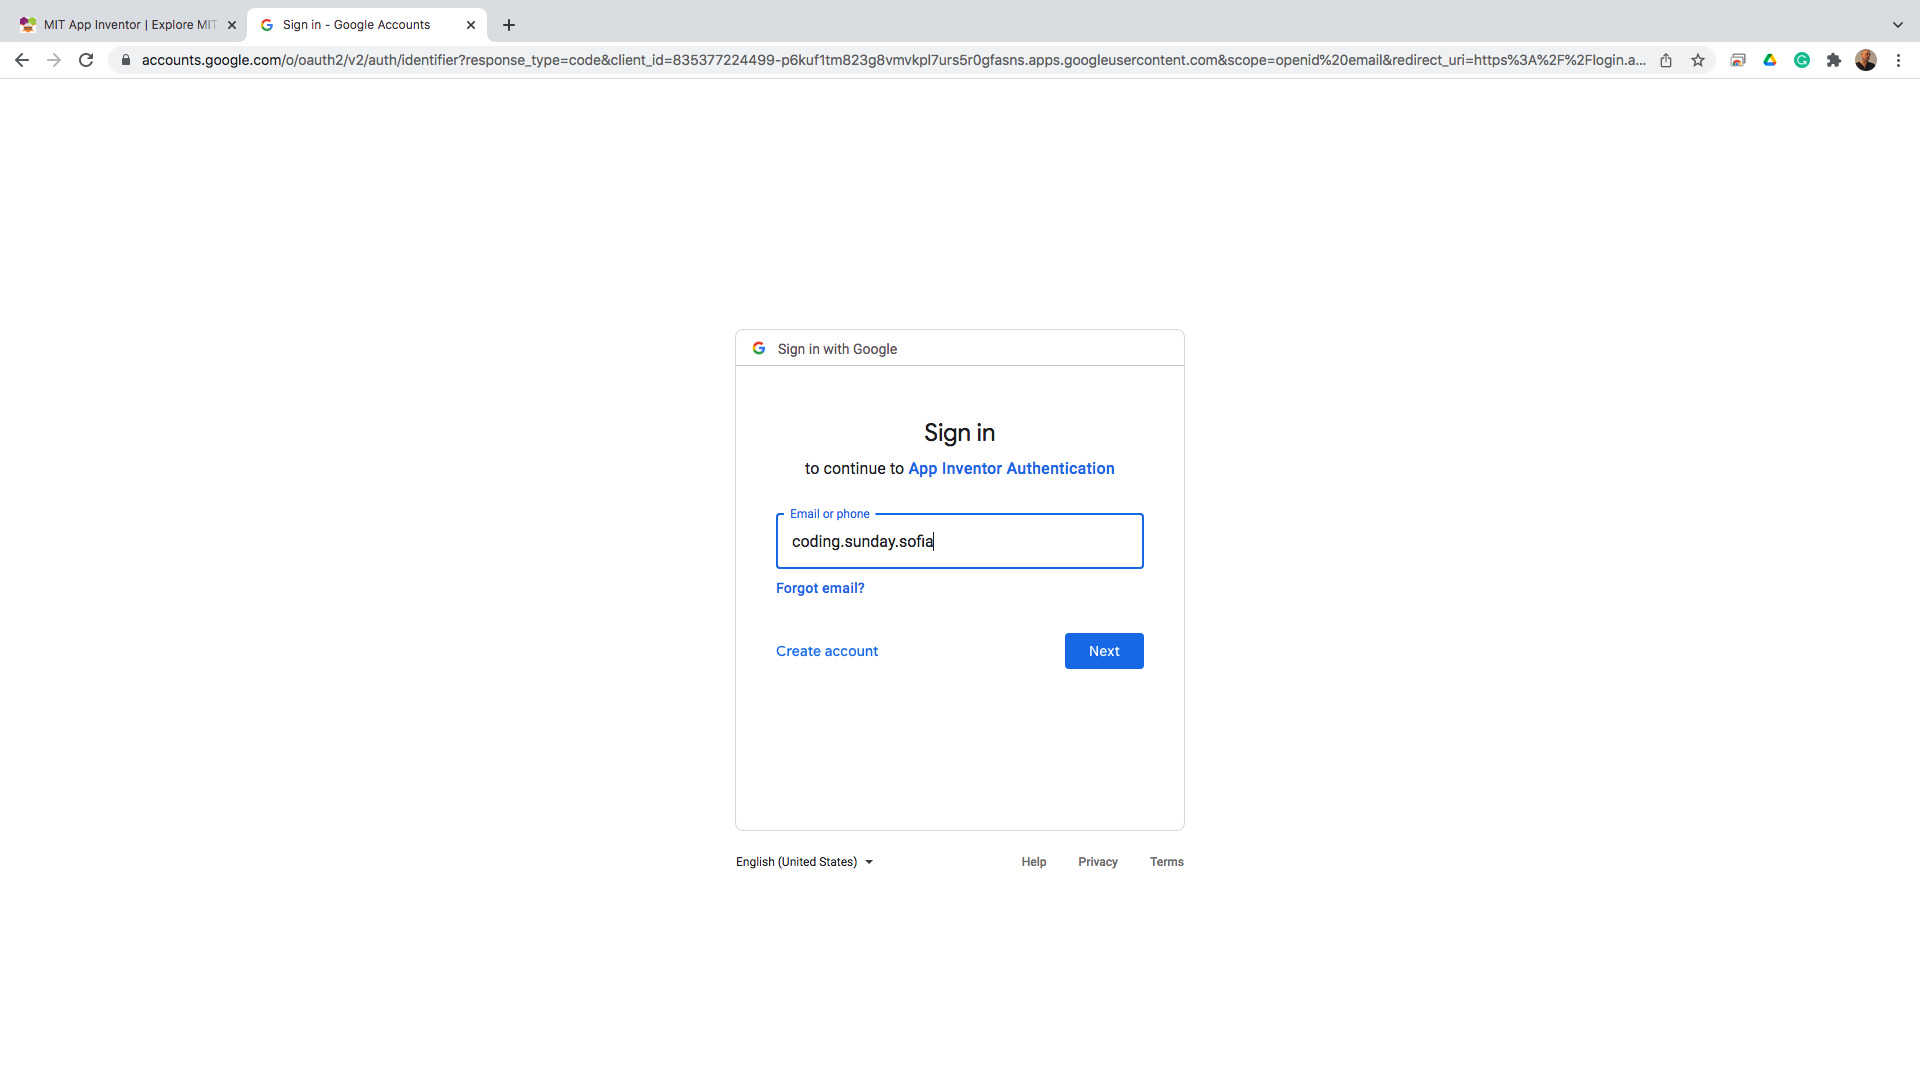
\includegraphics[width=1.0\linewidth,height=0.5\linewidth]{fig010022.png}
   \caption{Choosing a GMail user to log in}
\label{fig010022}
\end{figure}

After selecting a user to work within the App Inventor environment, this user must be authenticated by entering a password (Fig. \ref{fig010023}).

\begin{figure}[H]
   \centering
   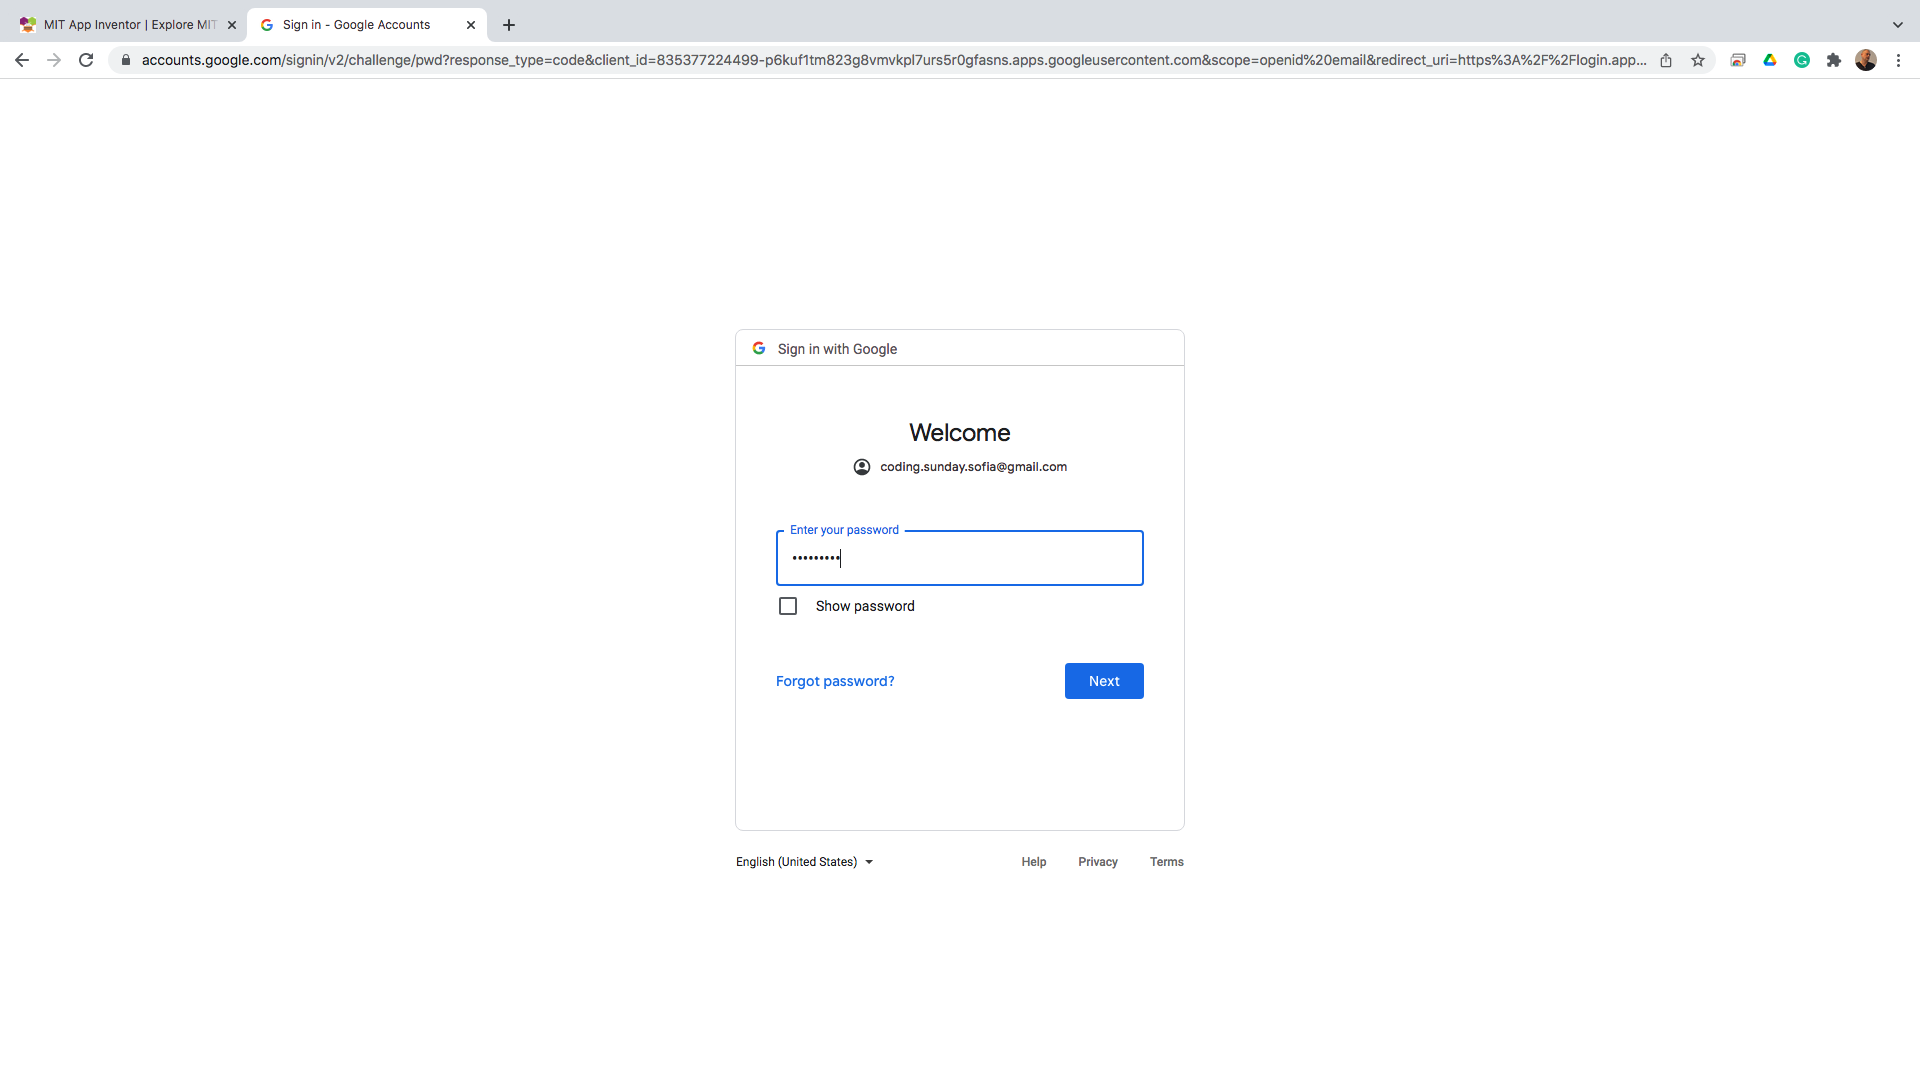
\includegraphics[width=1.0\linewidth,height=0.5\linewidth]{fig010023.png}
   \caption{User Authentication}
\label{fig010023}
\end{figure}

To be allowed to work in the App Inventor programming environment, the user's agreement with the general terms of the platform is required (Fig. \ref{fig010024}).

\begin{figure}[H]
   \centering
   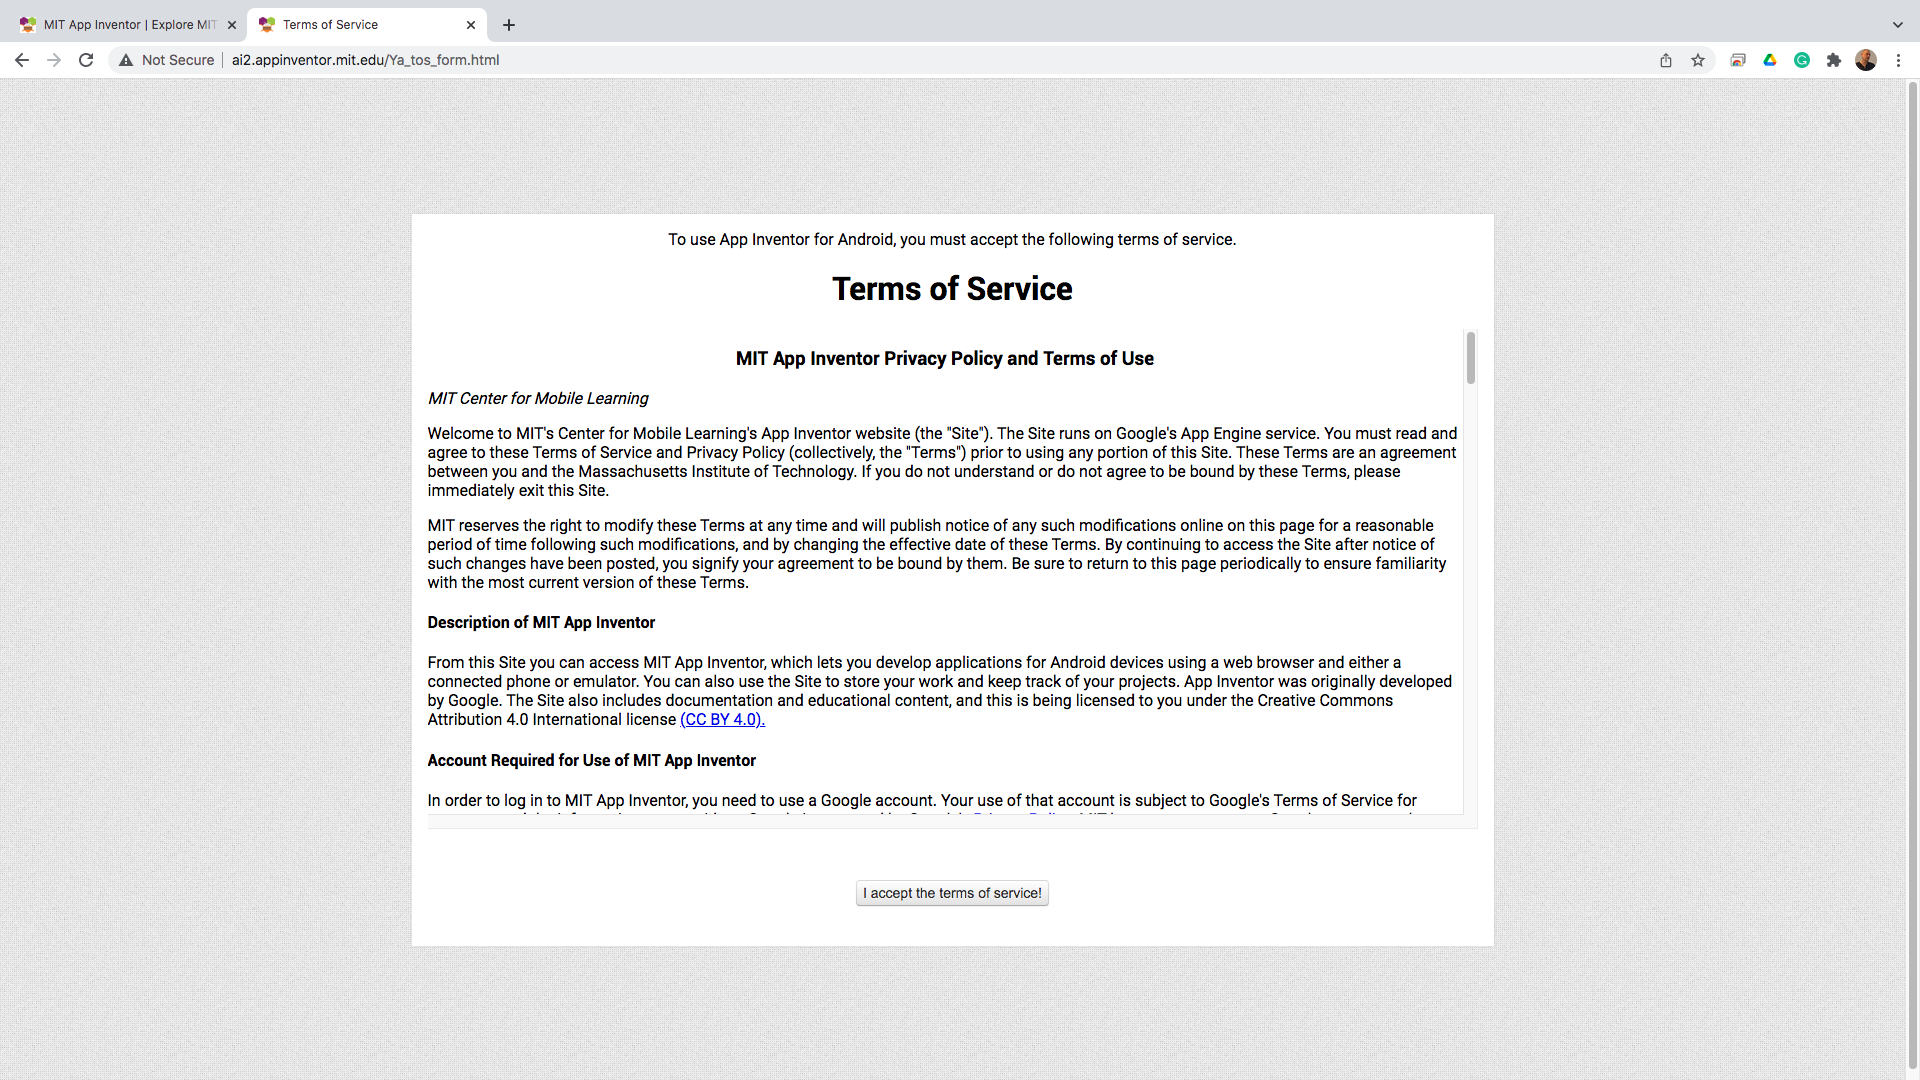
\includegraphics[width=1.0\linewidth,height=0.5\linewidth]{fig010024.png}
   \caption{General Terms of Use of the Program Environment}
\label{fig010024}
\end{figure}

Entering the programming environment ends with a welcome web page (Fig. \ref{fig010025}). This page presents more detailed information about the program environment, the type of instance launched, and the version.

\begin{figure}[H]
   \centering
   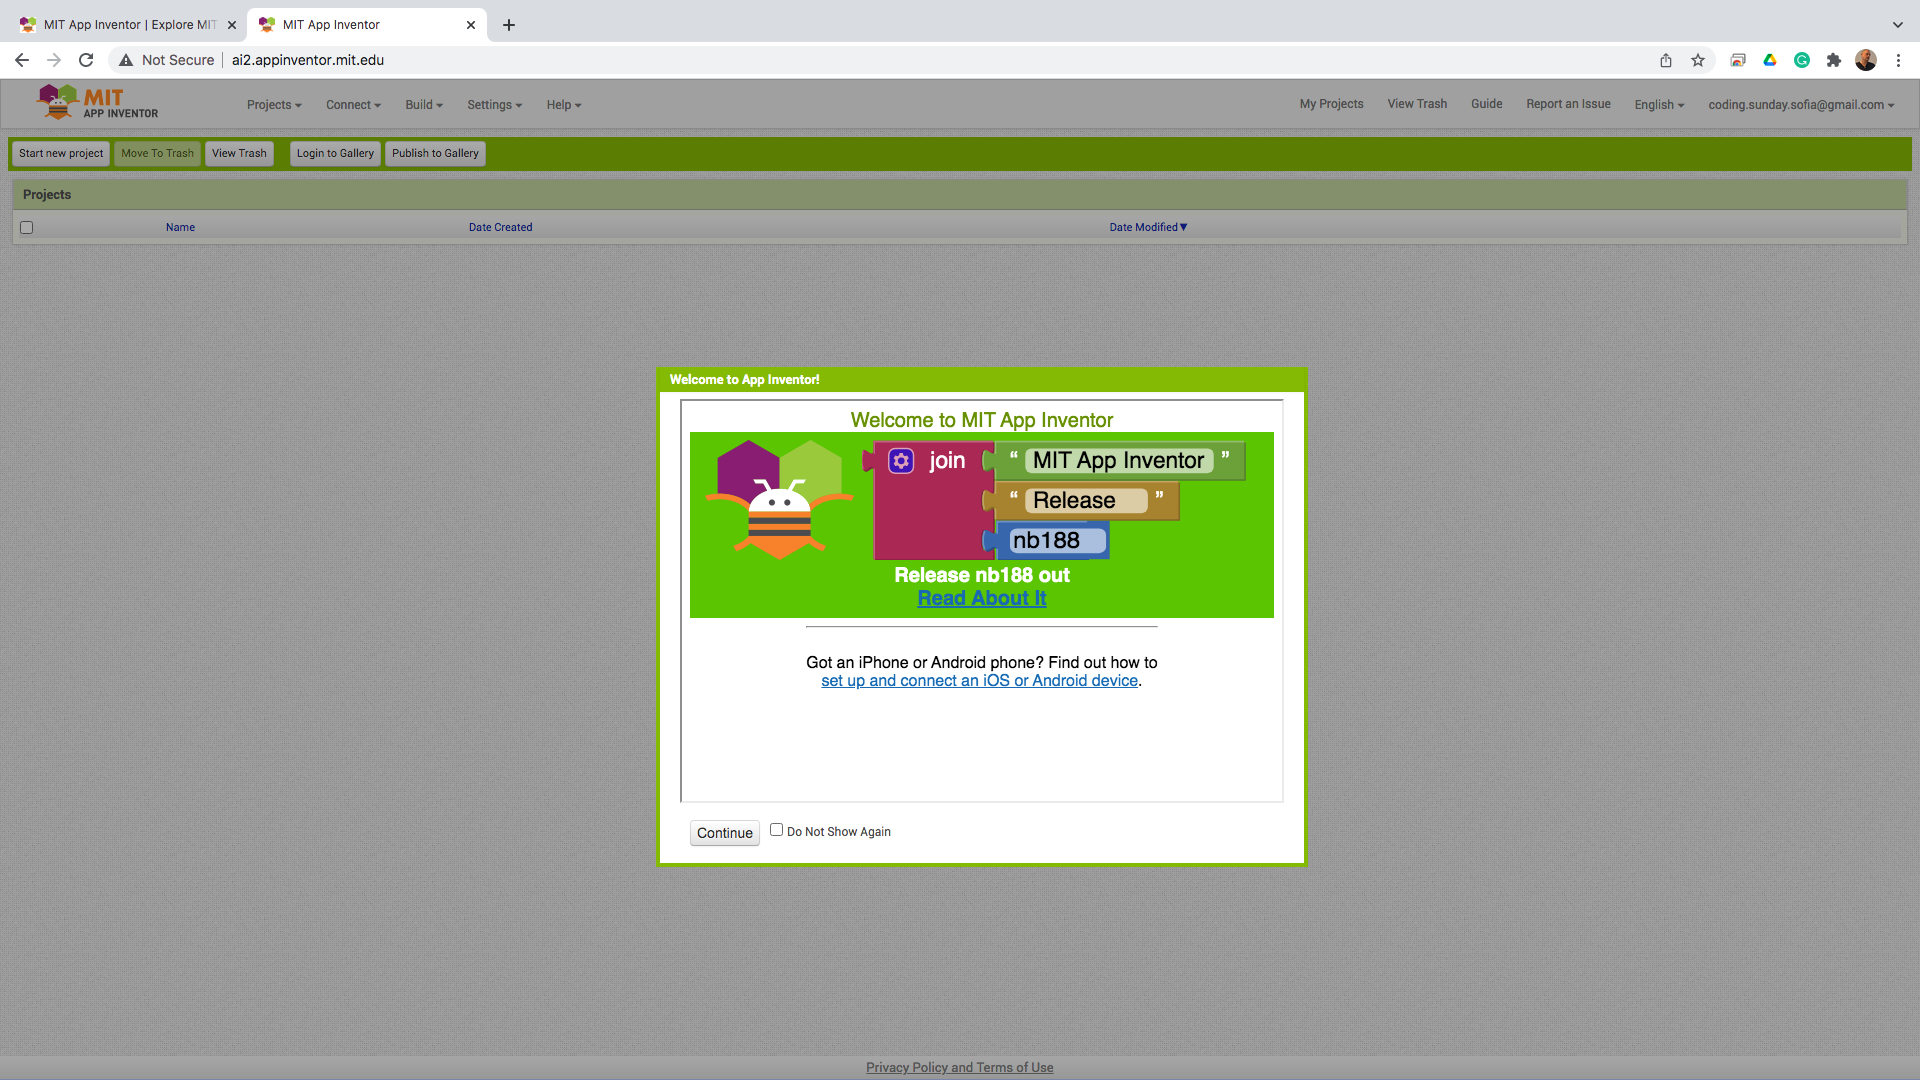
\includegraphics[width=1.0\linewidth,height=0.5\linewidth]{fig010025.png}
   \caption{Welcome Page}
\label{fig010025}
\end{figure}

The first option offered to the user is to choose from options to view several learning projects as an initial introduction to how to work with the programming environment (Fig. \ref{fig010026}).

\begin{figure}[H]
   \centering
   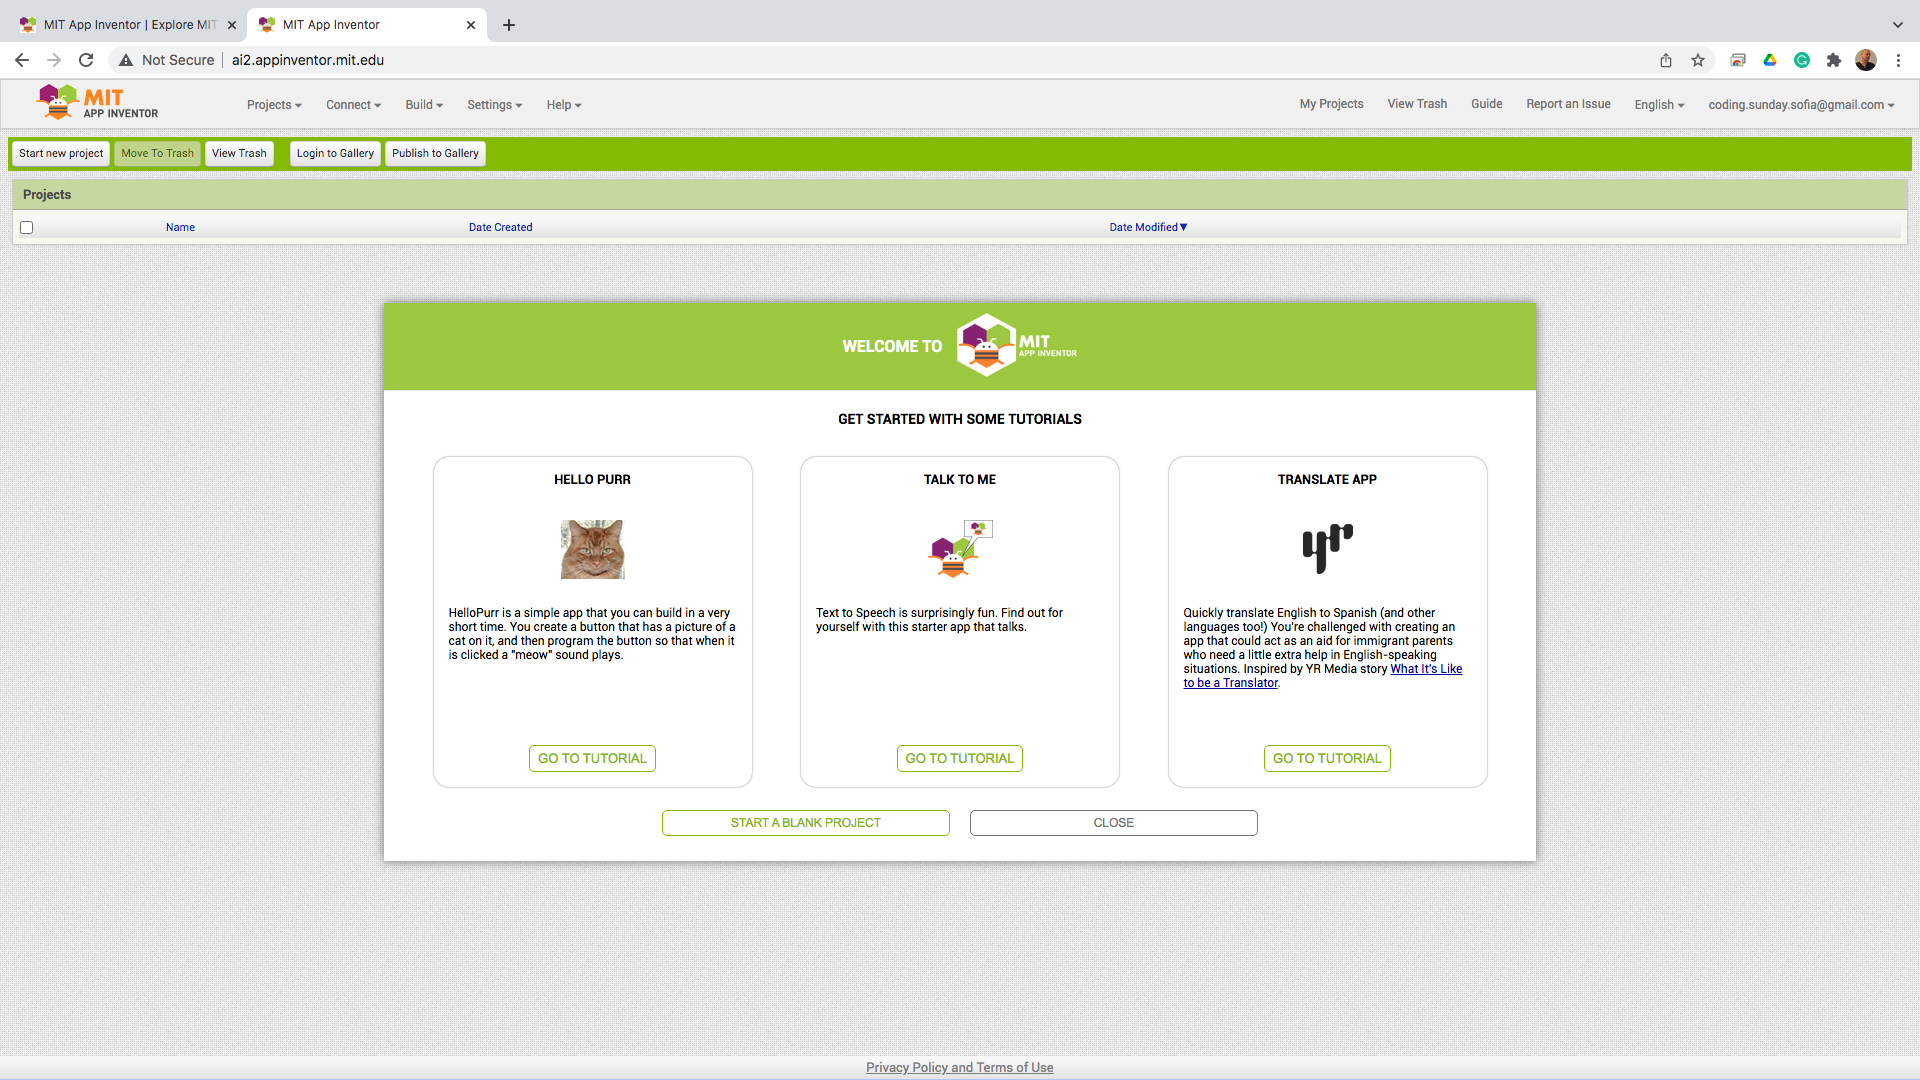
\includegraphics[width=1.0\linewidth,height=0.5\linewidth]{fig010026.png}
   \caption{Ability to choose learning projects}
\label{fig010026}
\end{figure}

If no learning project or the option to create an empty project is selected, the system directs the user to the page with a list of own projects (Fig. \ref{fig010027}).

\begin{figure}[H]
   \centering
   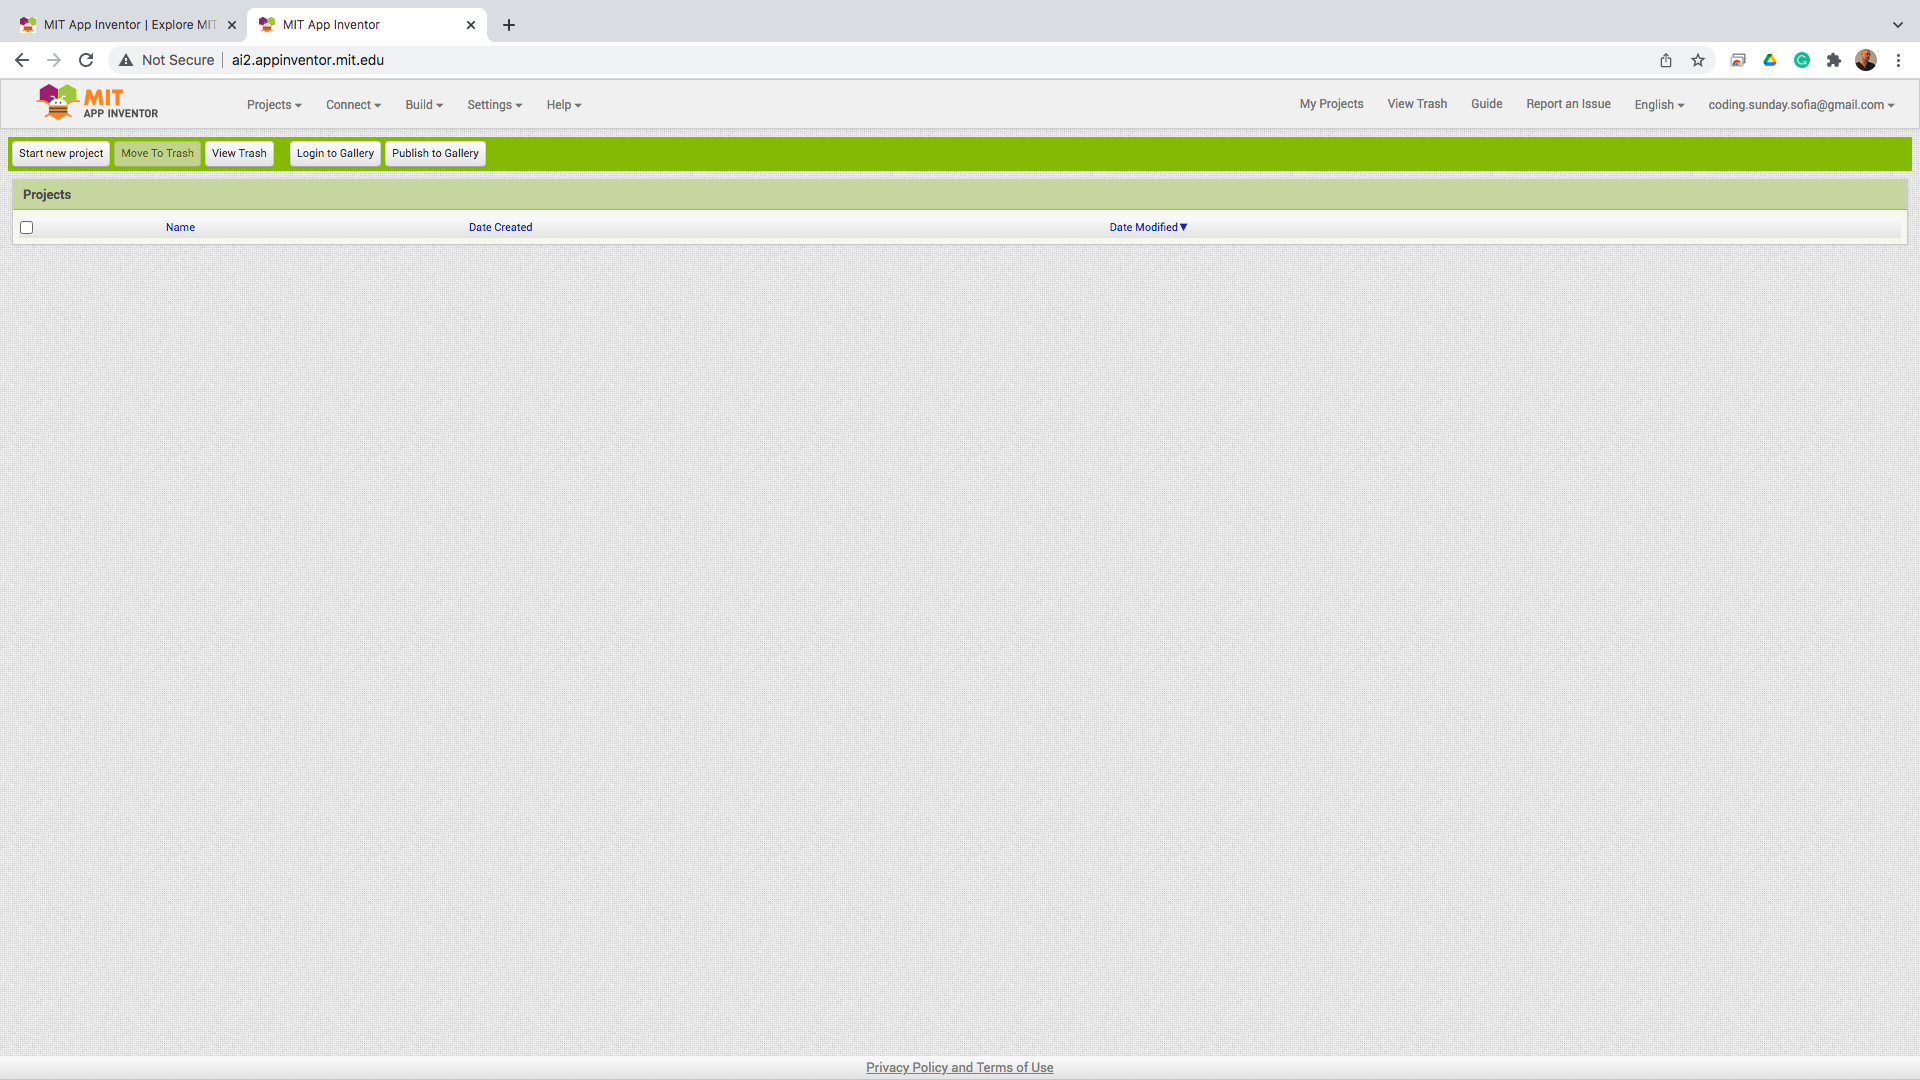
\includegraphics[width=1.0\linewidth,height=0.5\linewidth]{fig010027.png}
   \caption{Own Projects List Page}
\label{fig010027}
\end{figure}

Starting a new project happens from a button, at the top left, on the main work screen (Fig. \ref{fig010028}).

\begin{figure}[H]
   \centering
   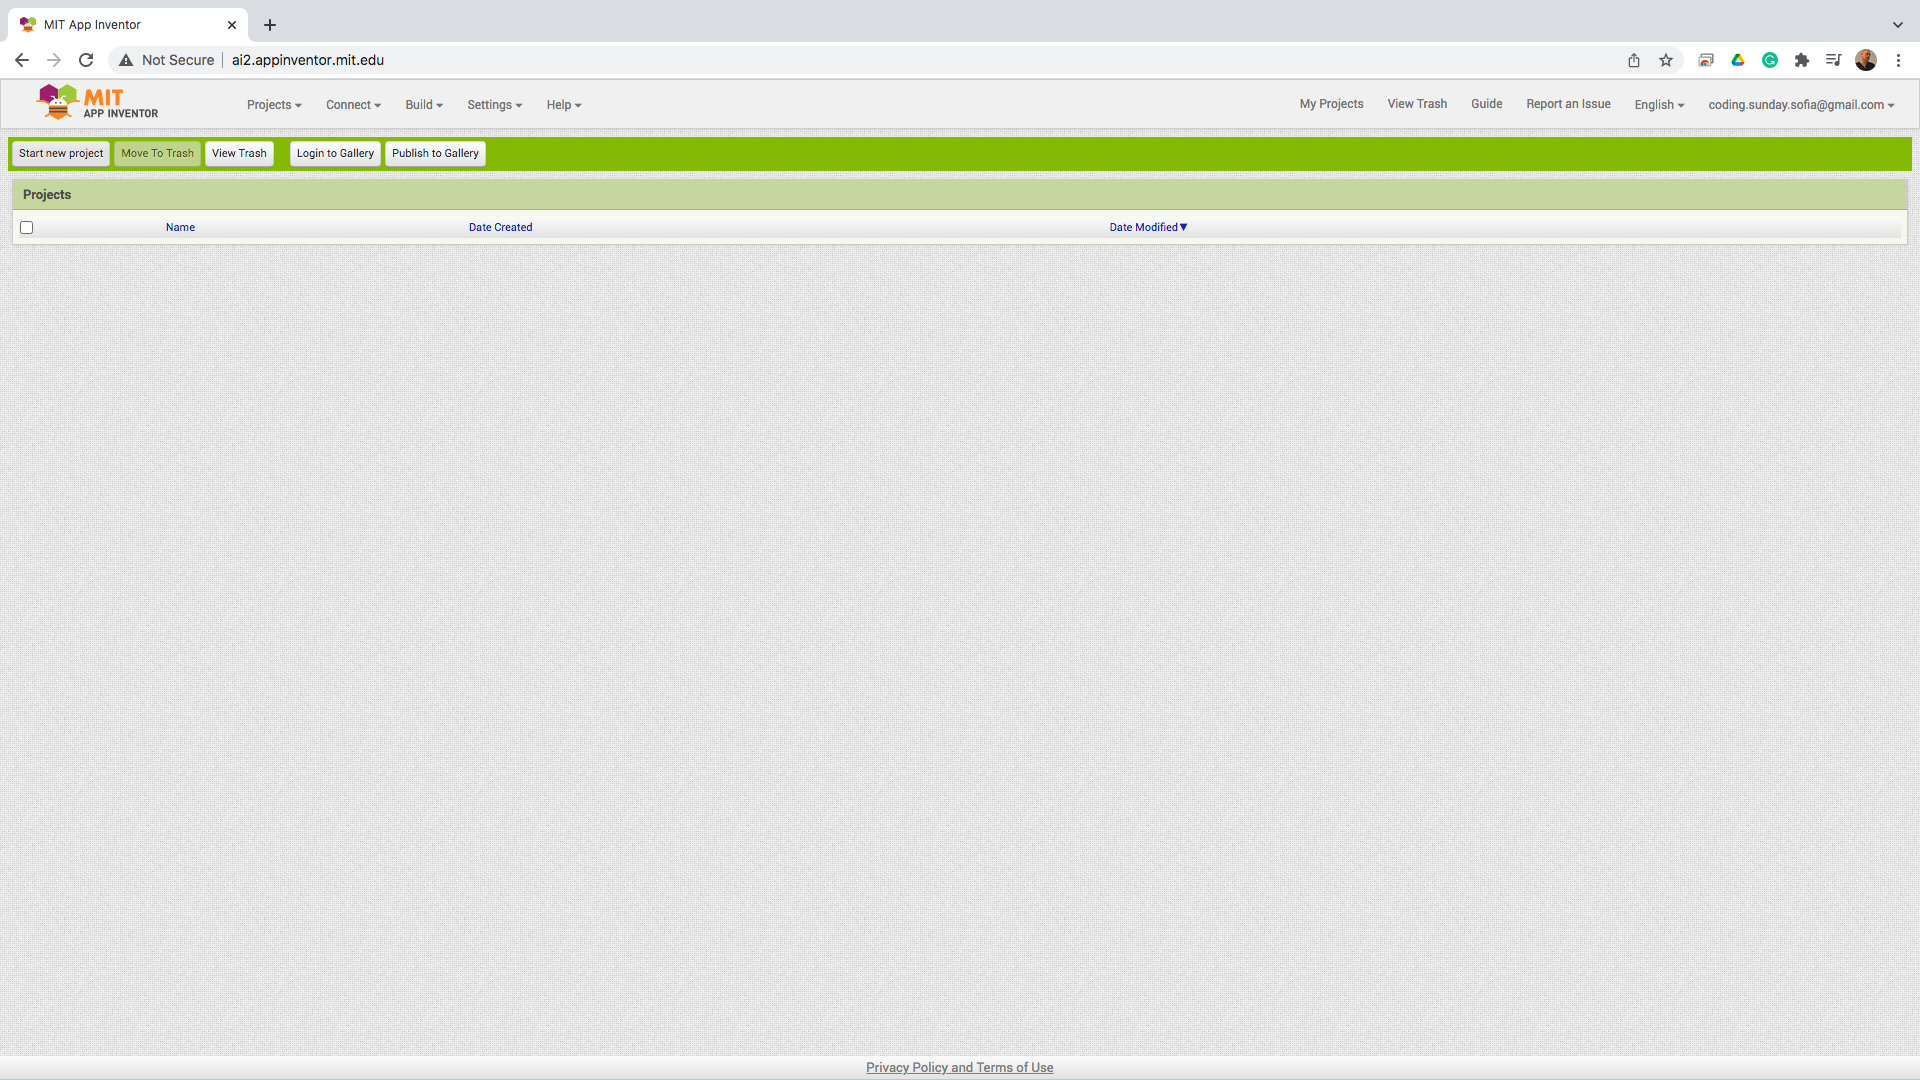
\includegraphics[width=1.0\linewidth,height=0.5\linewidth]{fig010028.png}
   \caption{Start New Project Button}
\label{fig010028}
\end{figure}

The App Inventor programming environment organizes work on programming code through projects. Each project must have an appropriate name set when the project is created (Fig. \ref{fig010029}).

\begin{figure}[H]
   \centering
   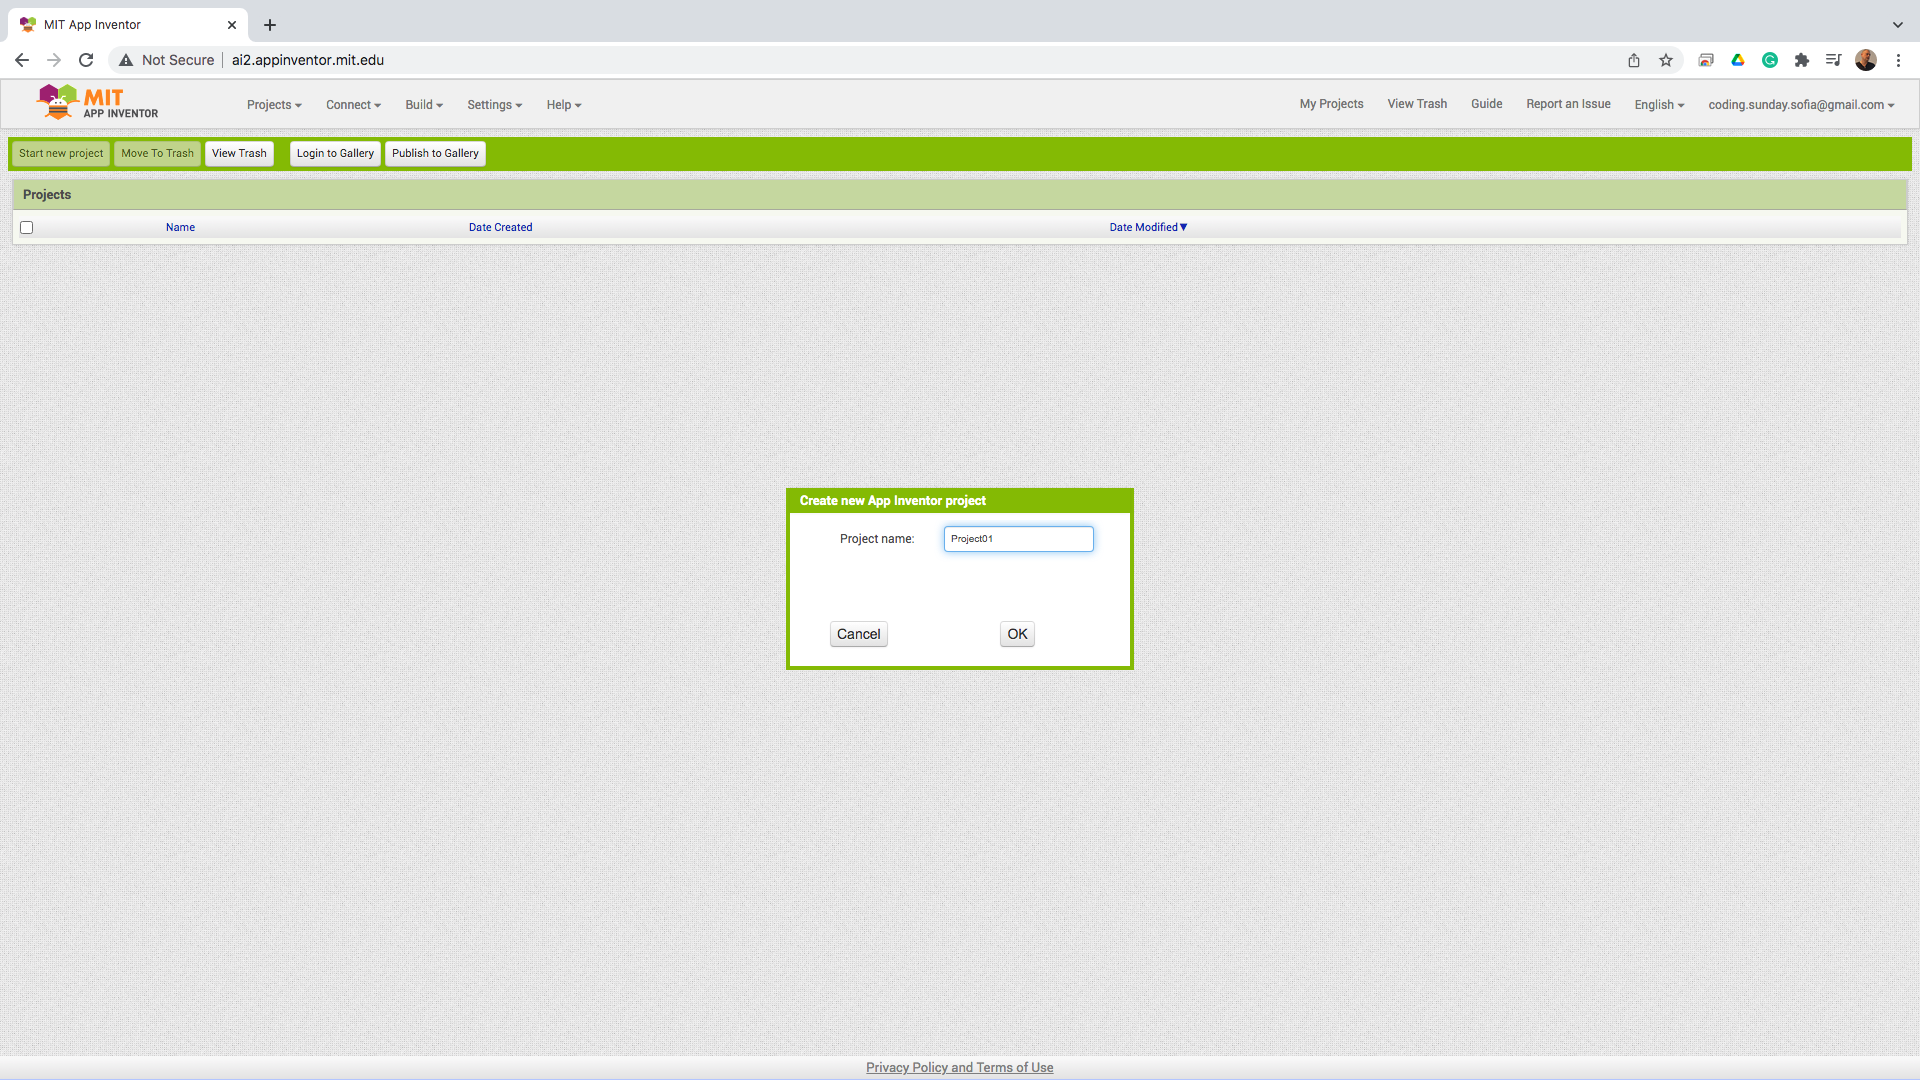
\includegraphics[width=1.0\linewidth,height=0.5\linewidth]{fig010029.png}
   \caption{Project Name}
\label{fig010029}
\end{figure}

After choosing a name, the programming environment visualizes the first working screen, giving the possibility to design the visual user interface (Fig. \ref{fig010030}). Creating the graphical user interface happens by dragging the various visual controls into the main work area.

\begin{figure}[H]
   \centering
   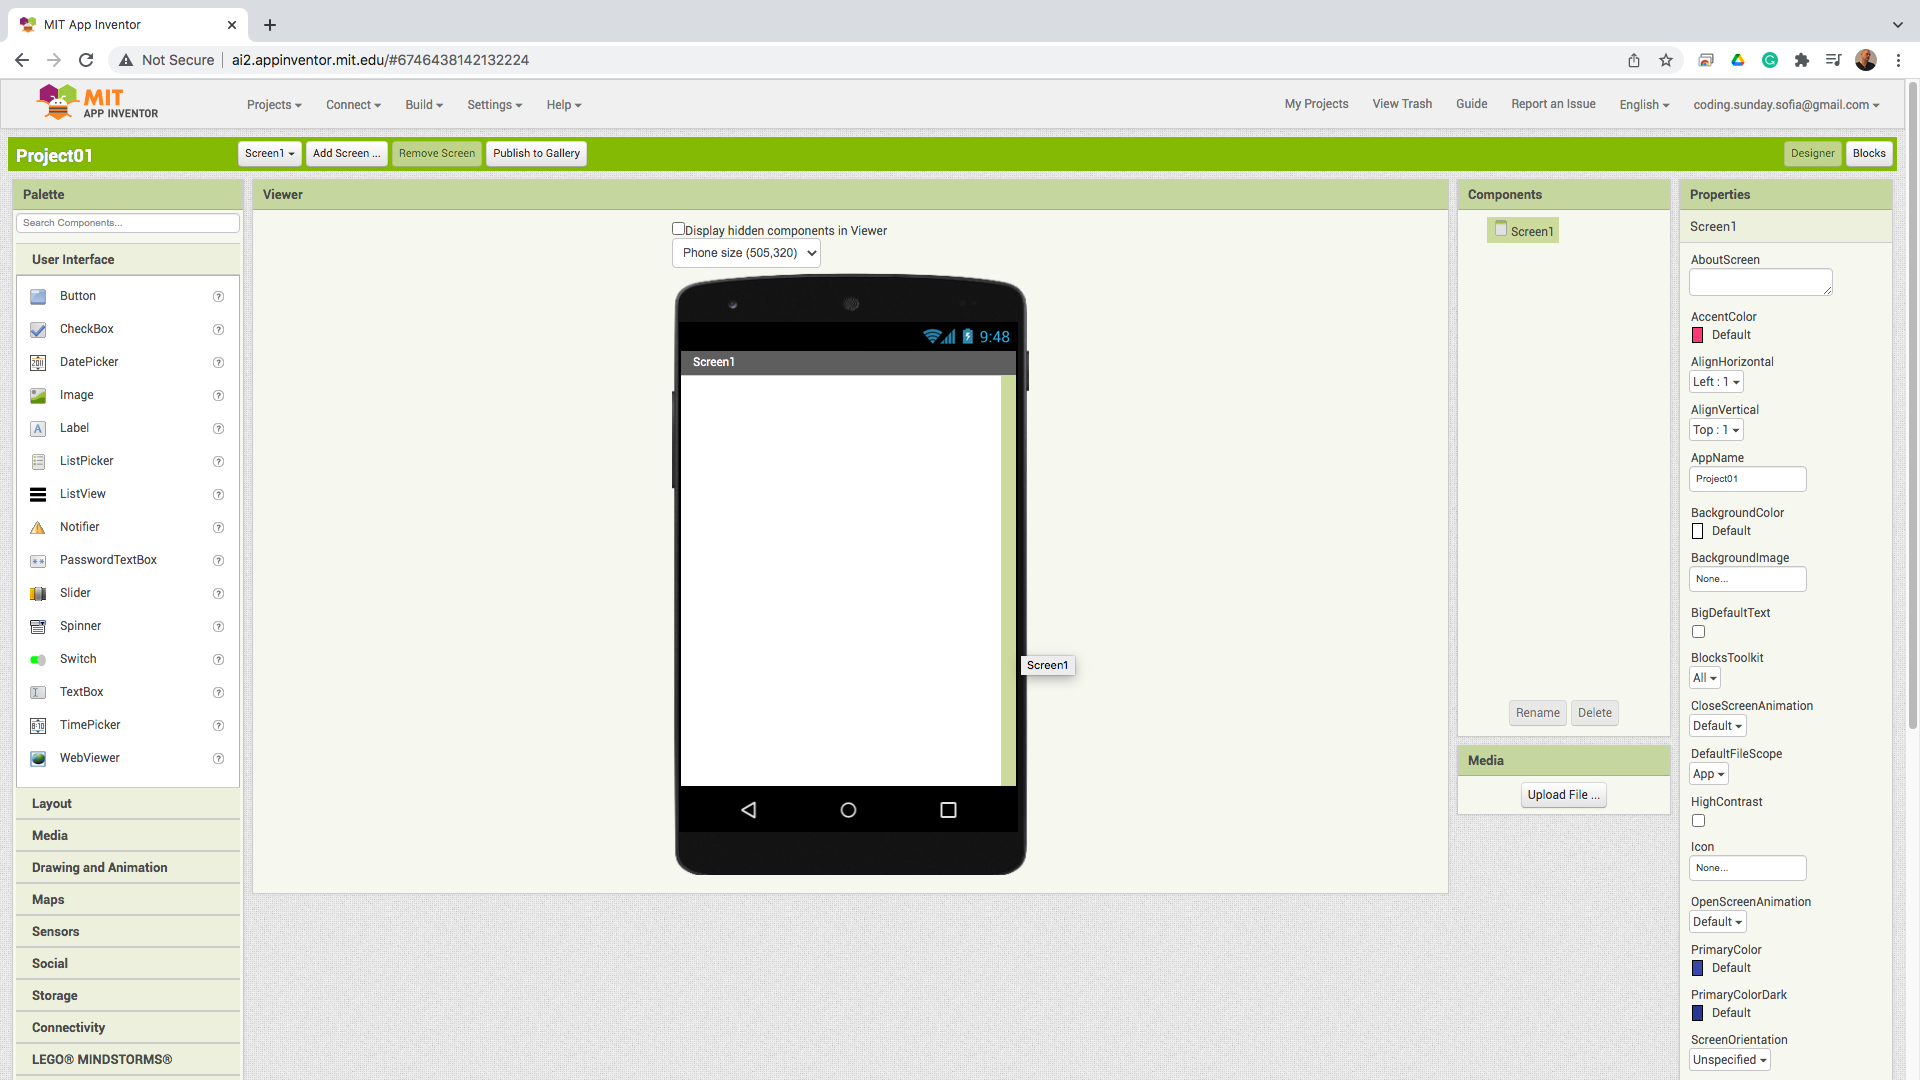
\includegraphics[width=1.0\linewidth,height=0.5\linewidth]{fig010030.png}
   \caption{Design view of the development environment}
\label{fig010030}
\end{figure}

One of the most basic visual controls is the button. Represents a designated area in the visual field with a text label or icon to visually represent the action performed after the button is pressed. One button is used to demonstrate the process of working with the compiled program code (Fig. \ref{fig010031}).

\begin{figure}[H]
   \centering
   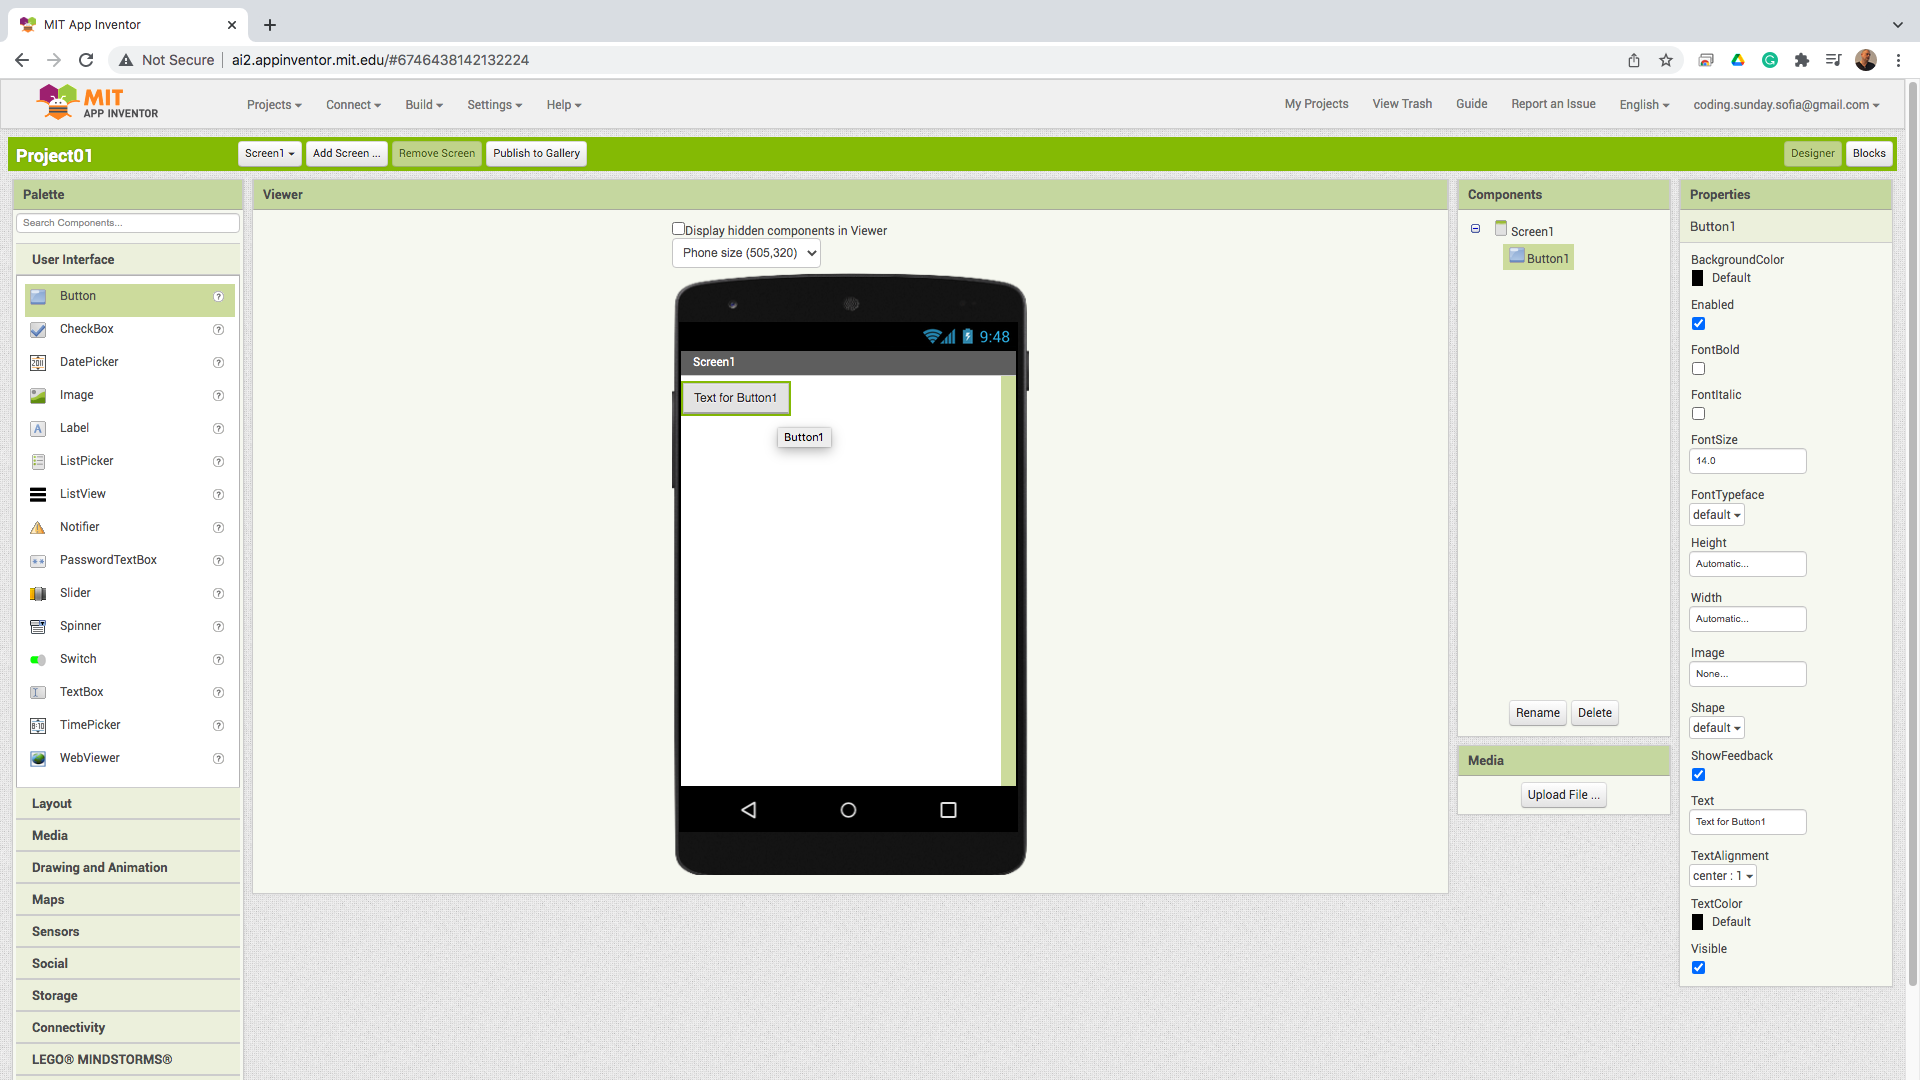
\includegraphics[width=1.0\linewidth,height=0.5\linewidth]{fig010031.png}
   \caption{Place Button}
\label{fig010031}
\end{figure}

It is essential for people using the software application that the buttons have maximally expressive names. In this case, the goal is for the button to be pressed and a specific action to follow. For this reason, the name of the button is just "Push" (Fig. \ref{fig010031}).

\begin{figure}[H]
   \centering
   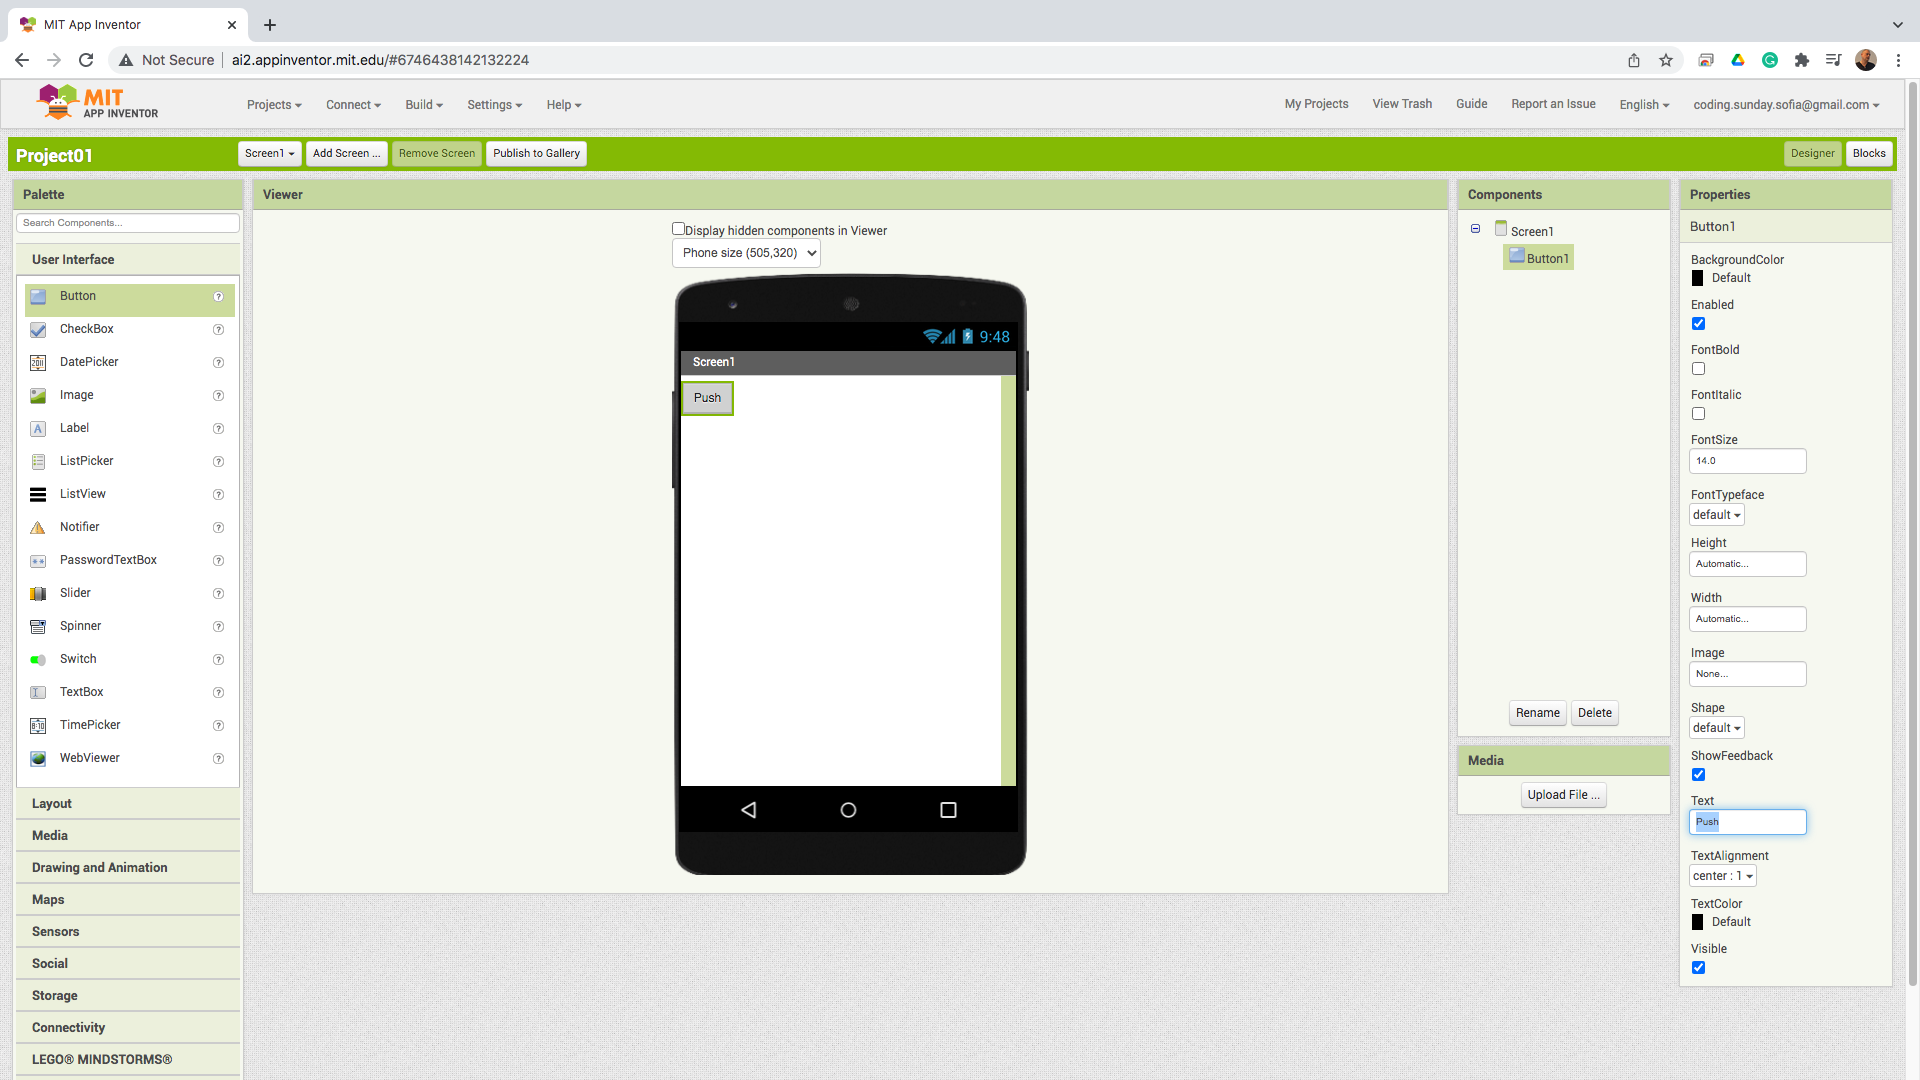
\includegraphics[width=1.0\linewidth,height=0.5\linewidth]{fig010032.png}
   \caption{Select text on button}
\label{fig010032}
\end{figure}

Unlike the Scratch programming environment, App Inventor's program instructions are cut as a puzzle in a separate work screen (Fig. \ref{fig010033}).

\begin{figure}[H]
   \centering
   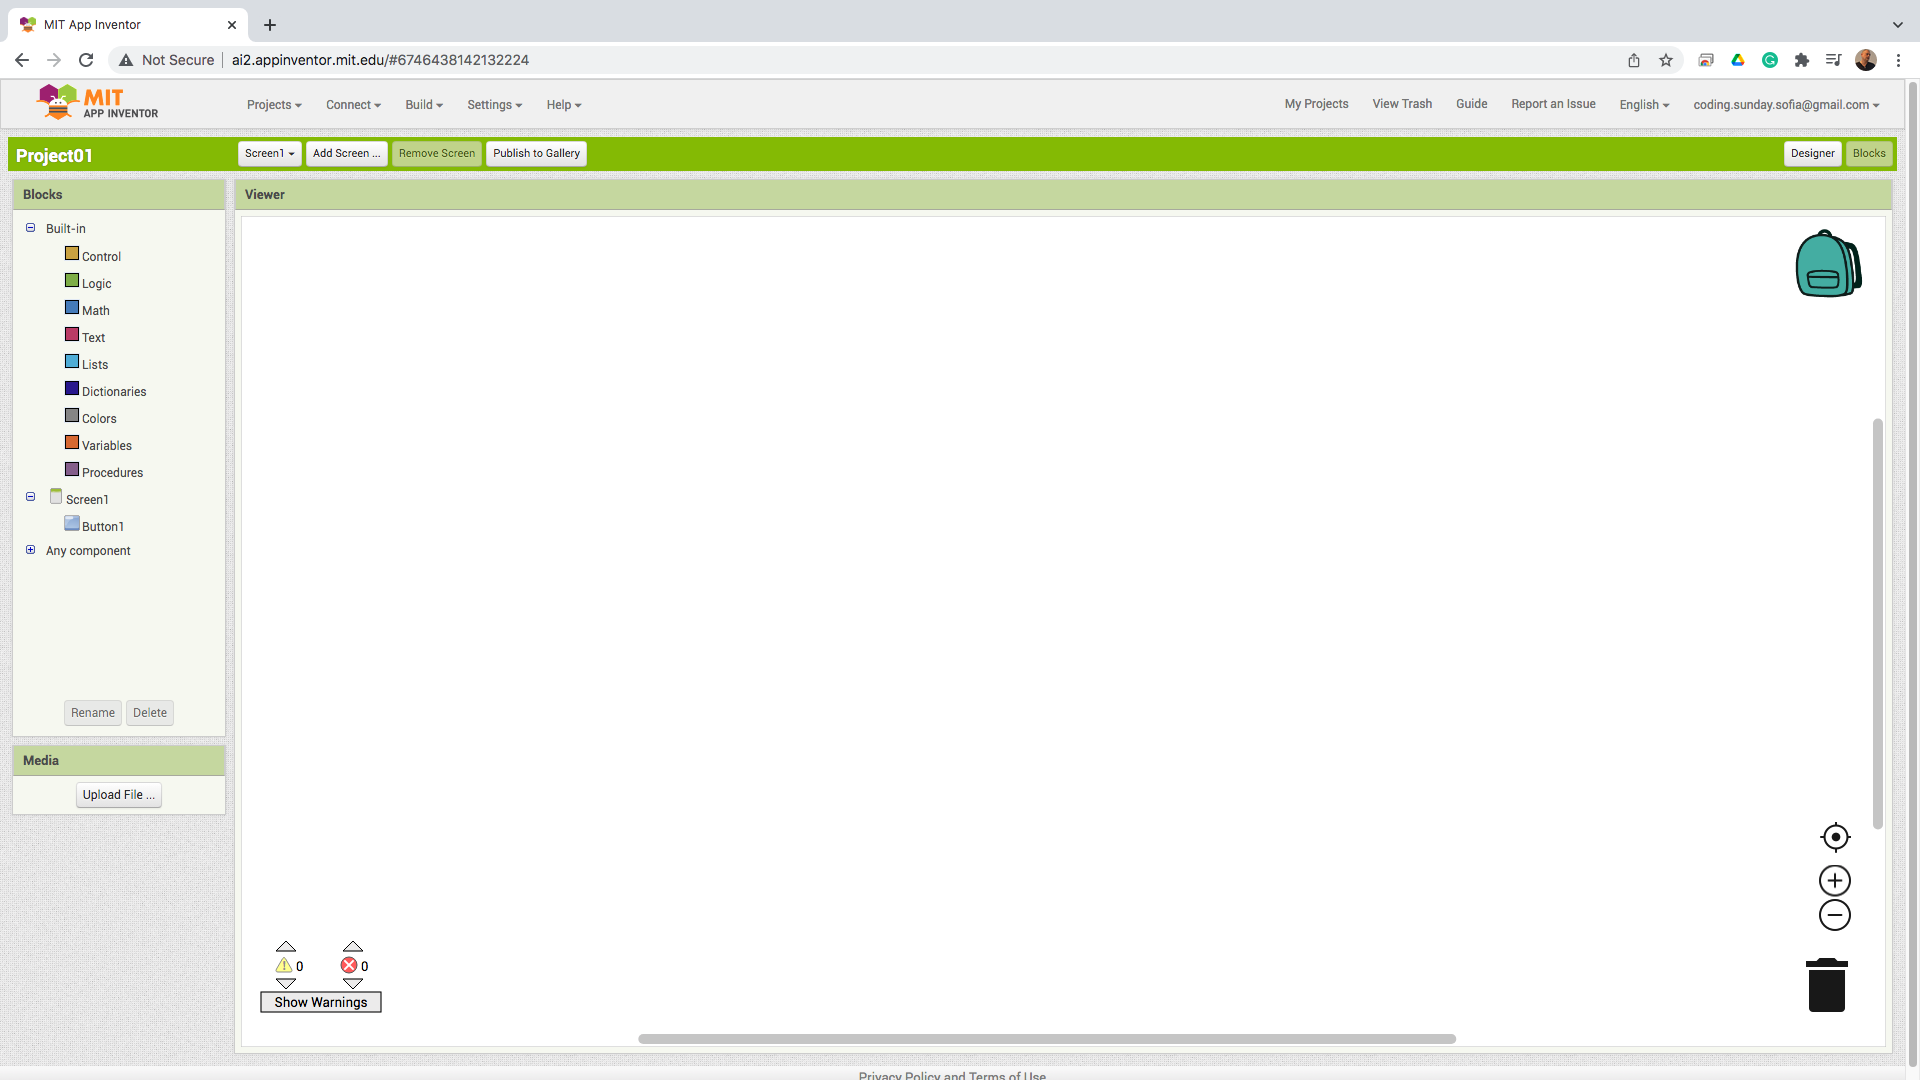
\includegraphics[width=1.0\linewidth,height=0.5\linewidth]{fig010033.png}
   \caption{Program view of the development environment}
\label{fig010033}
\end{figure}

Since the graphical user interface has only a single component (a button), some instructions can only be executed with this visual component. Unlike Scratch, where the program has an initial starting point and a final endpoint, App Inventor's instructions are ordered according to the principle of occurring events. When the program starts running, it visualizes the graphical user interface and expects the device user to perform some action (Fig. \ref{fig010034}).

\begin{figure}[H]
   \centering
   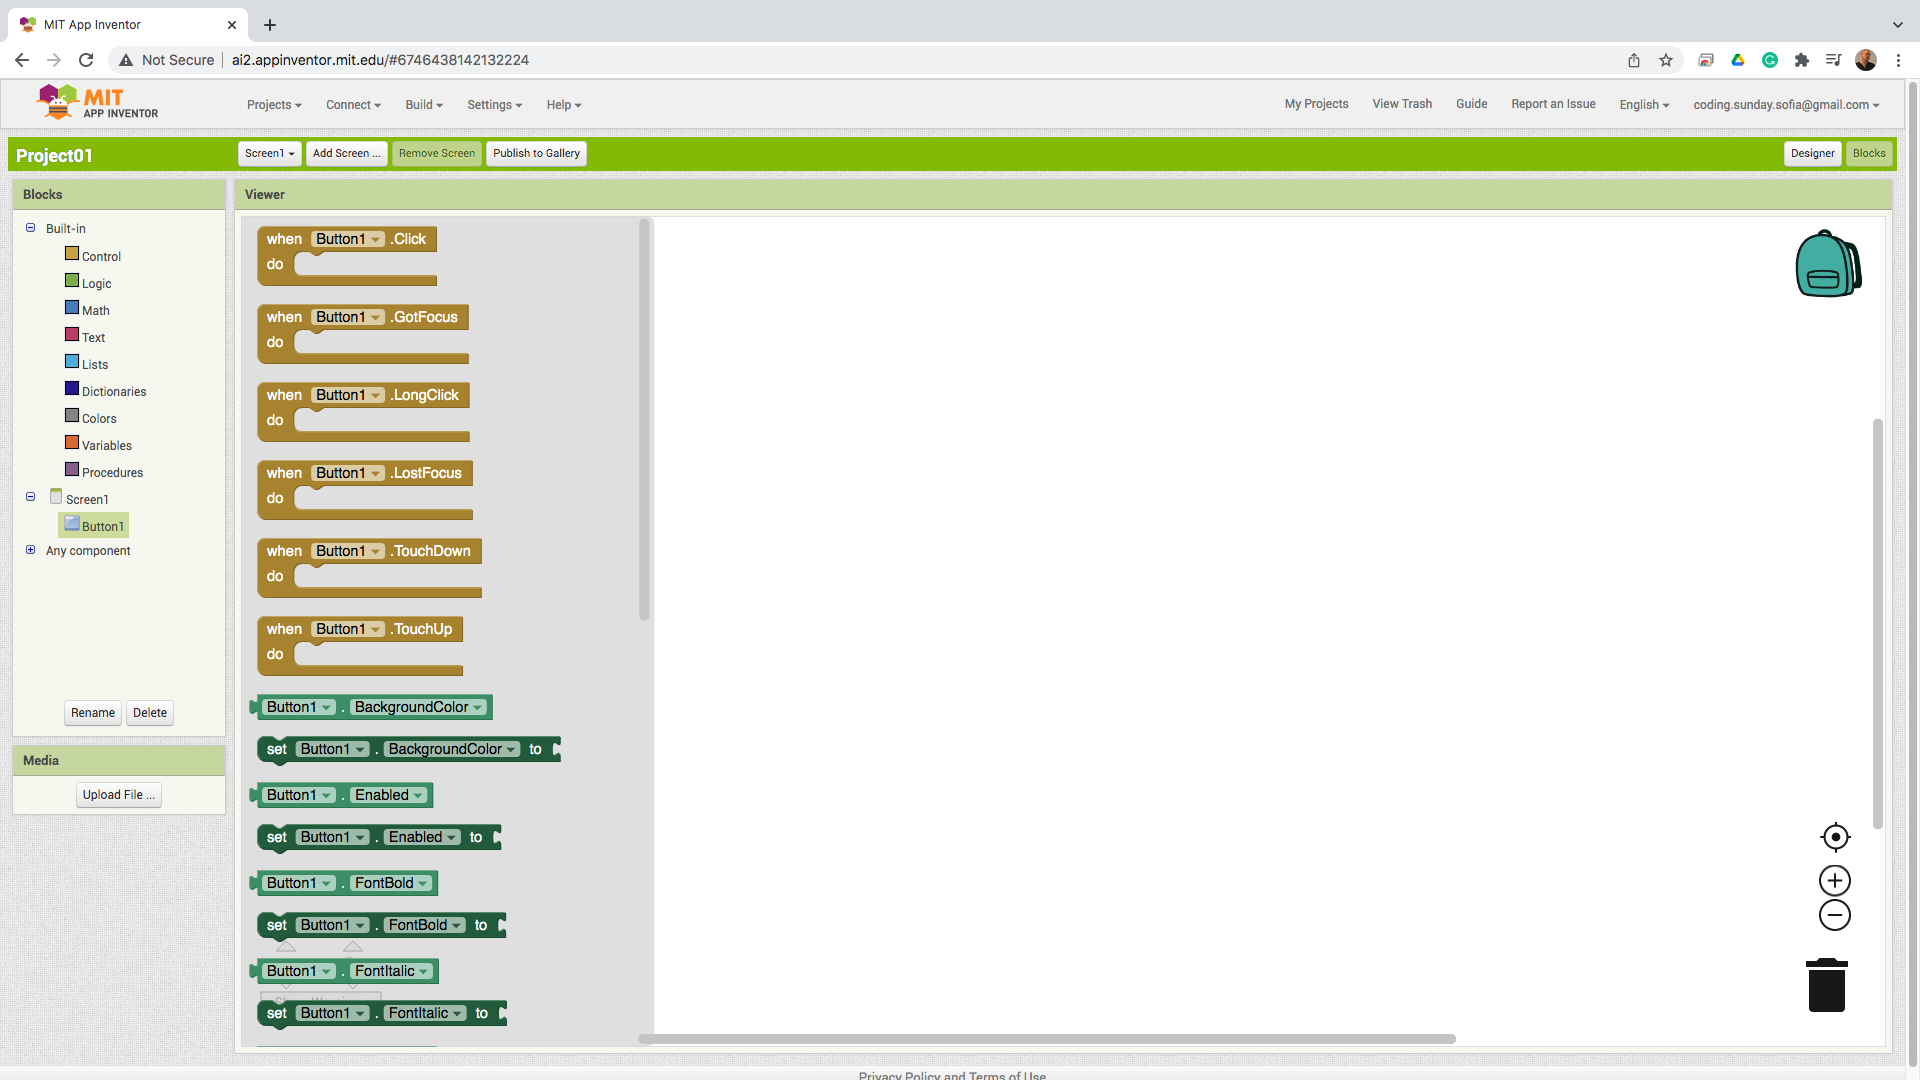
\includegraphics[width=1.0\linewidth,height=0.5\linewidth]{fig010034.png}
   \caption{List of instructions}
\label{fig010034}
\end{figure}

Such an action could be pressing a button. On the App Inventor side, the pressed button generates an event (event), for which event-specific activities of the program are selected (Fig. \ref{fig010035}).

\begin{figure}[H]
   \centering
   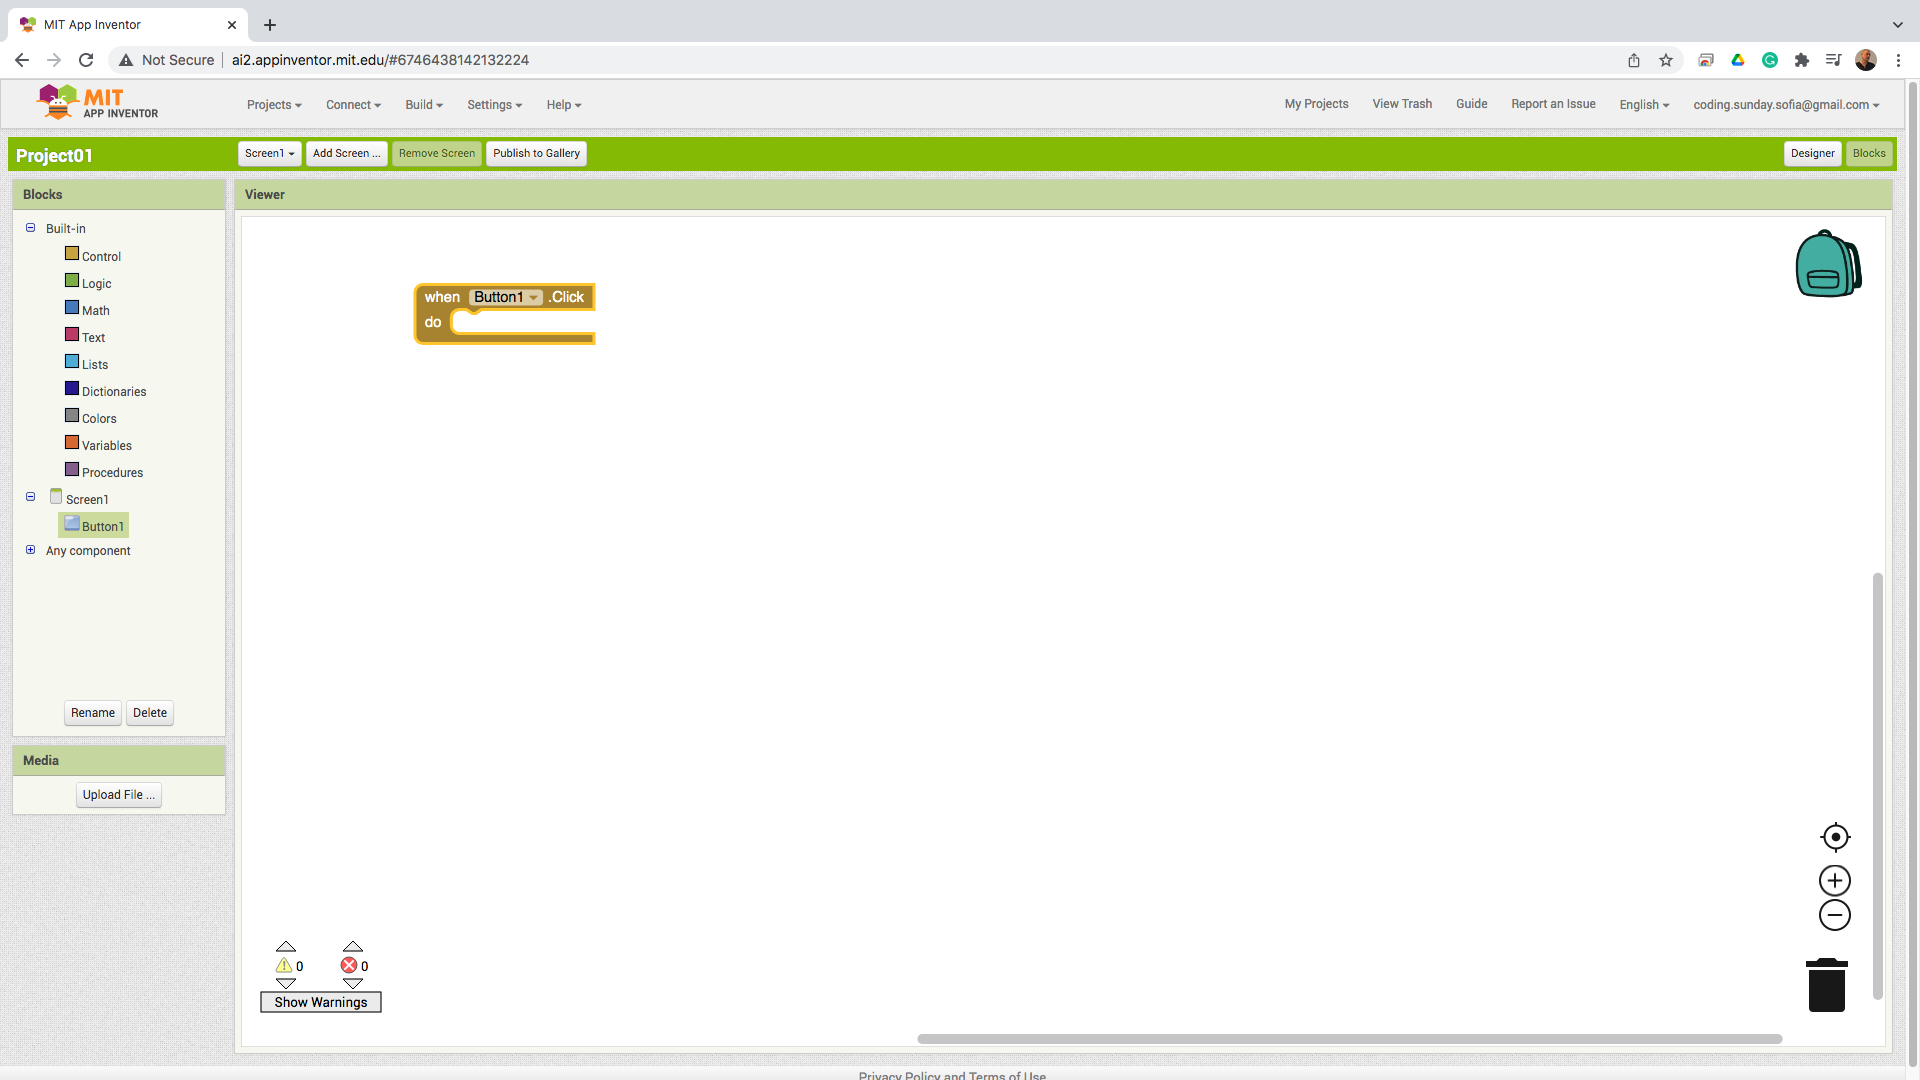
\includegraphics[width=1.0\linewidth,height=0.5\linewidth]{fig010035.png}
   \caption{Select event for button press}
\label{fig010035}
\end{figure}

The button press event is visualized as a puzzle piece containing a slot into which the instructions to be executed can be arranged (Fig. \ref{fig010036}).

\begin{figure}[H]
   \centering
   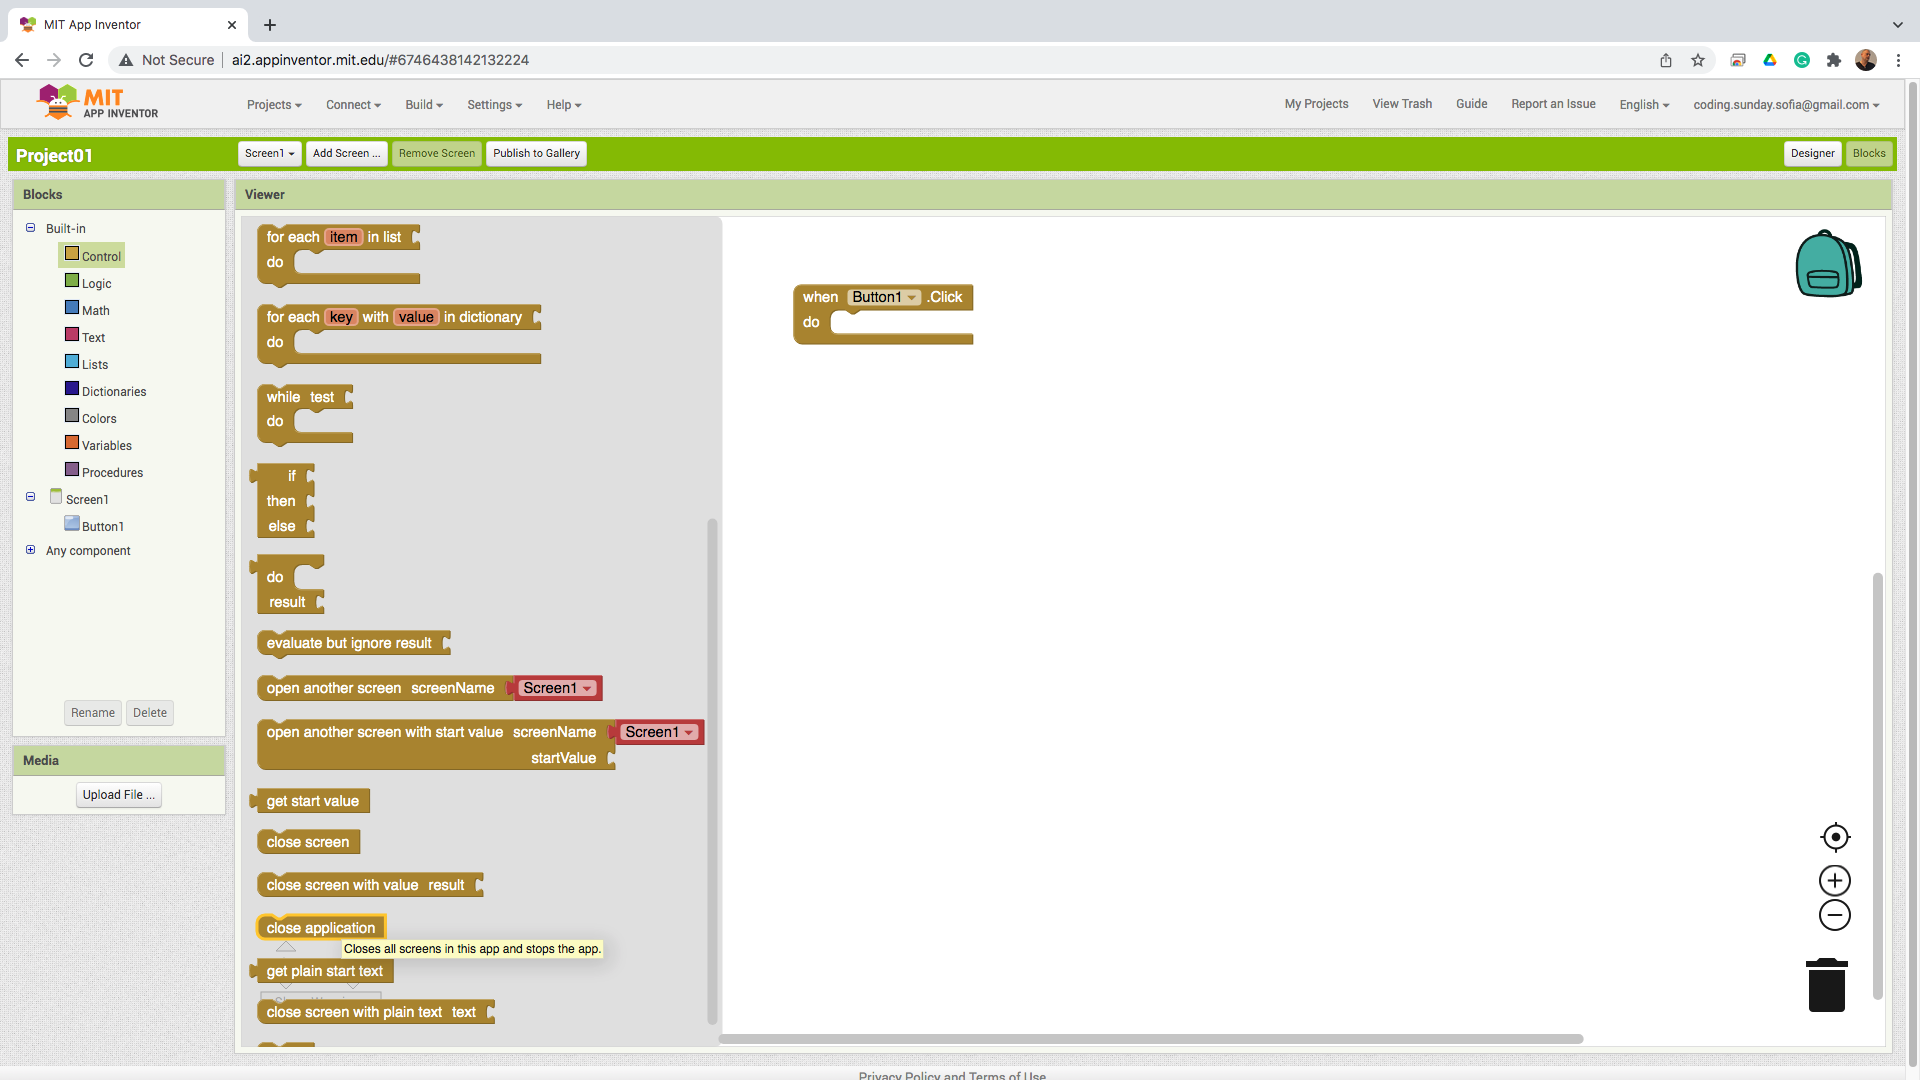
\includegraphics[width=1.0\linewidth,height=0.5\linewidth]{fig010036.png}
   \caption{Select action when the button is pressed}
\label{fig010036}
\end{figure}

The most straightforward action that can be performed after pressing the button is to stop the program and close the window of the application being developed (Fig. \ref{fig010037}).

\begin{figure}[H]
   \centering
   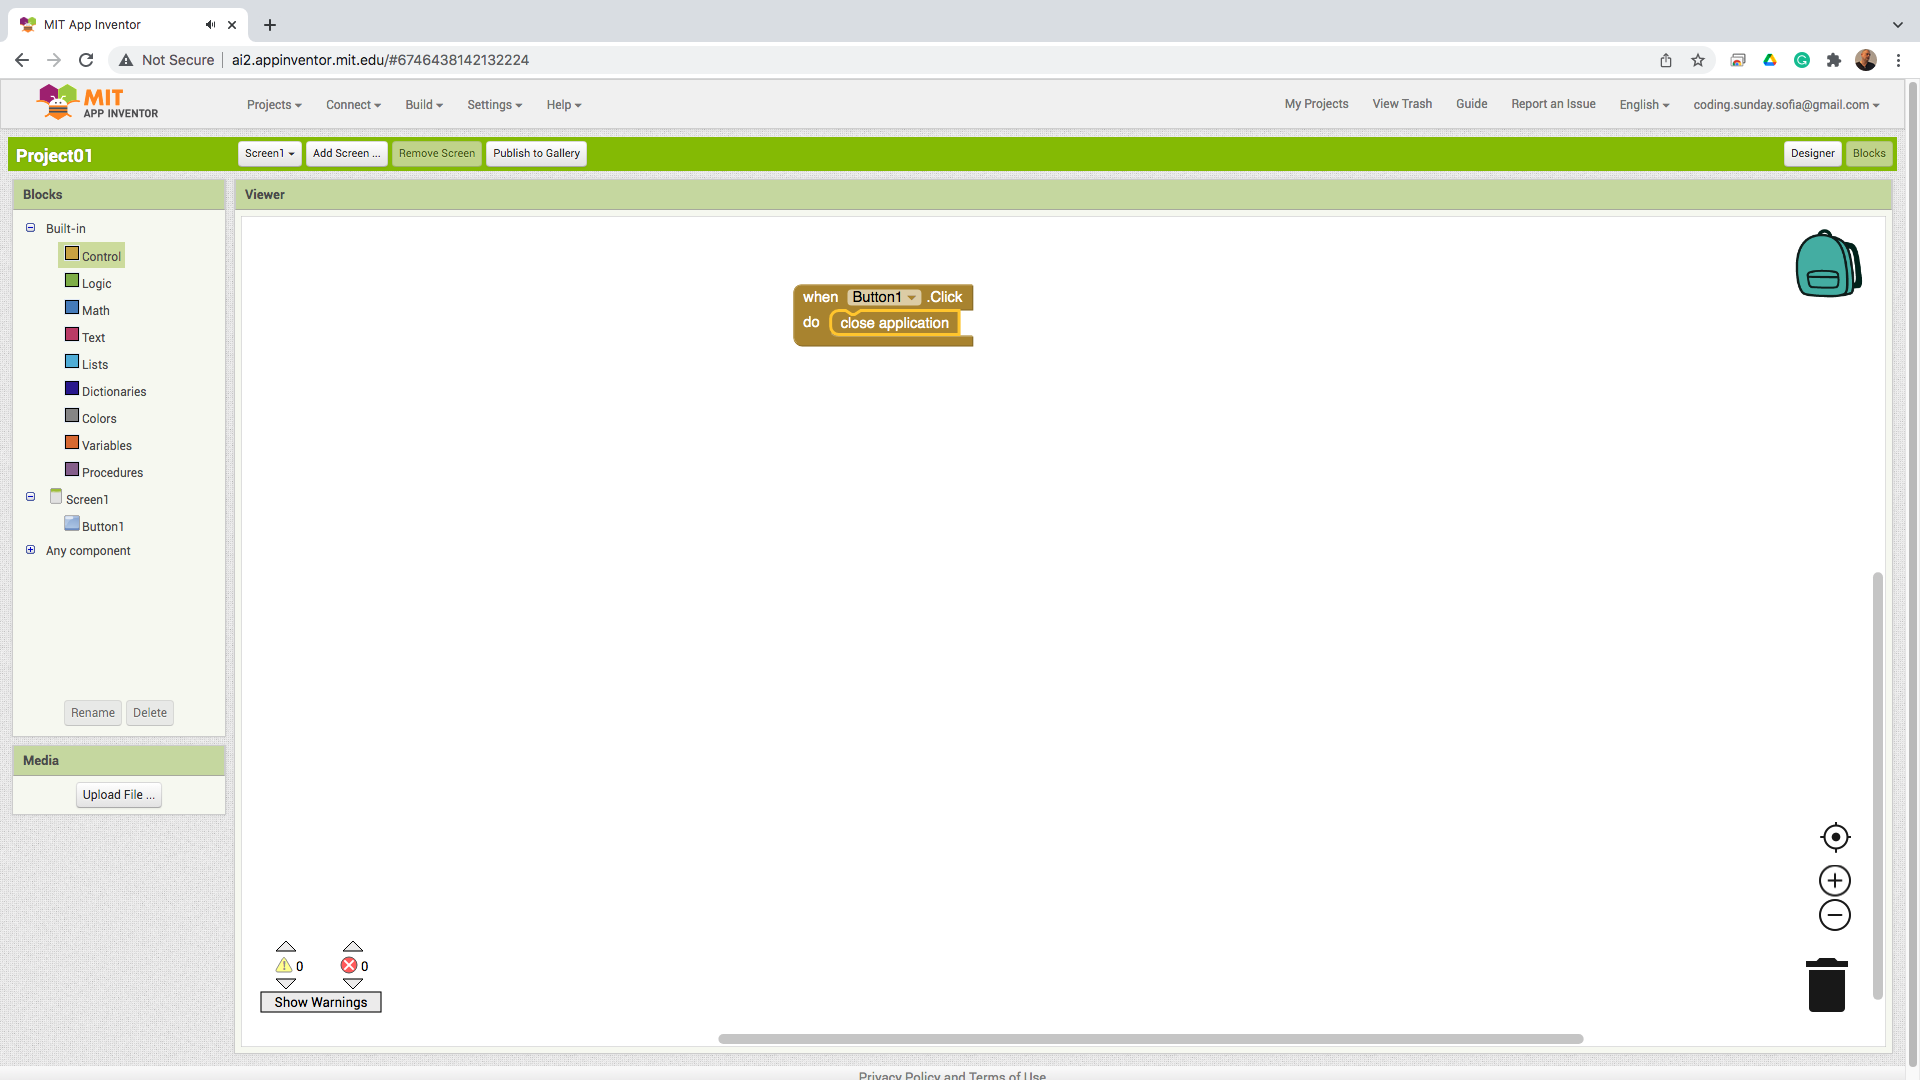
\includegraphics[width=1.0\linewidth,height=0.5\linewidth]{fig010037.png}
   \caption{Close application on button click}
\label{fig010037}
\end{figure}

After the graphical programming interface is designed and the desired instructions are arranged, the code is compiled, and the complete installation package for the written program is built (Fig. \ref{fig010038}).

\begin{figure}[H]
   \centering
   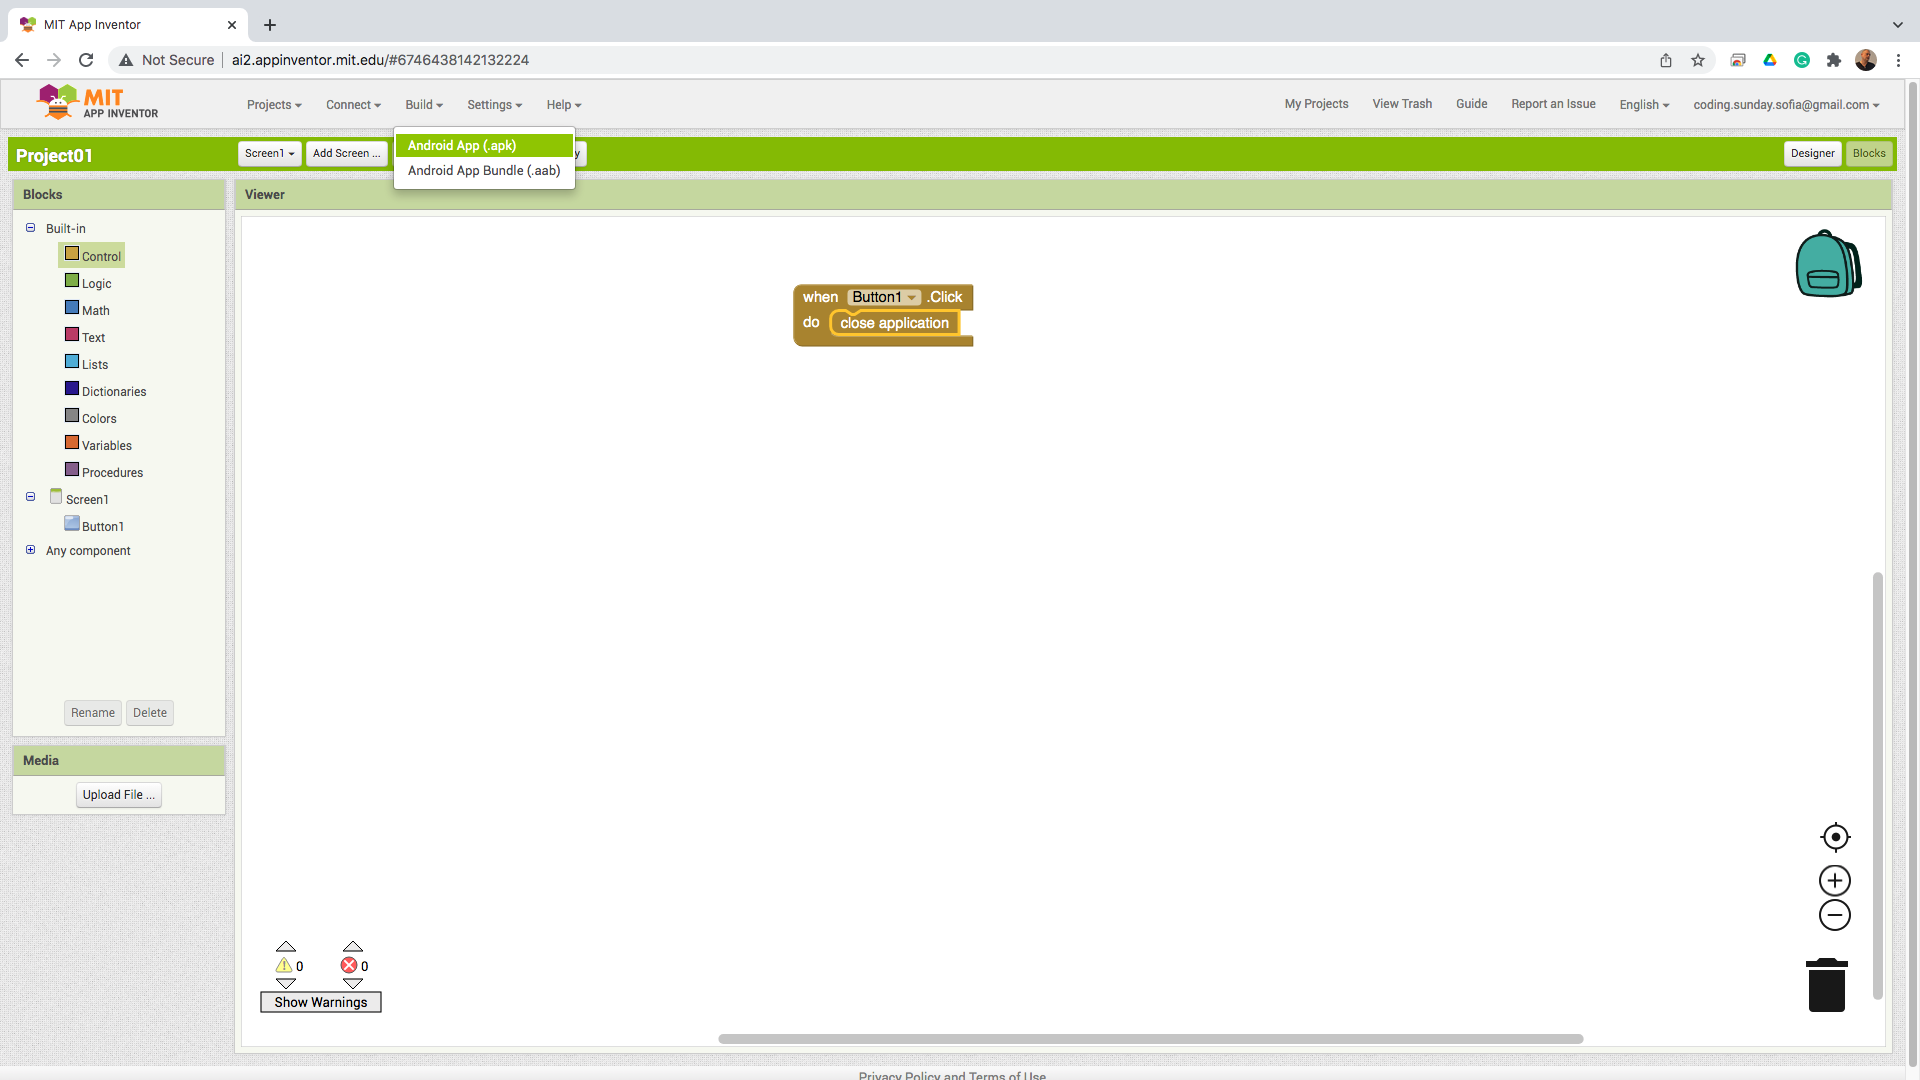
\includegraphics[width=1.0\linewidth,height=0.5\linewidth]{fig010038.png}
   \caption{Mobile App Build Menu}
\label{fig010038}
\end{figure}

A fundamental difference between Scratch and App Inventor is that the result of the execution of the programming instructions in Scratch is visible in the workspace of the programming environment itself, while in App Inventor, the installation package of the program is compiled in the cloud structure. It must be downloaded and installed on a mobile device. Compiling and building the installation package requires a particular computing time, visualized as a progress bar (Fig. \ref{fig010039}).

\begin{figure}[H]
   \centering
   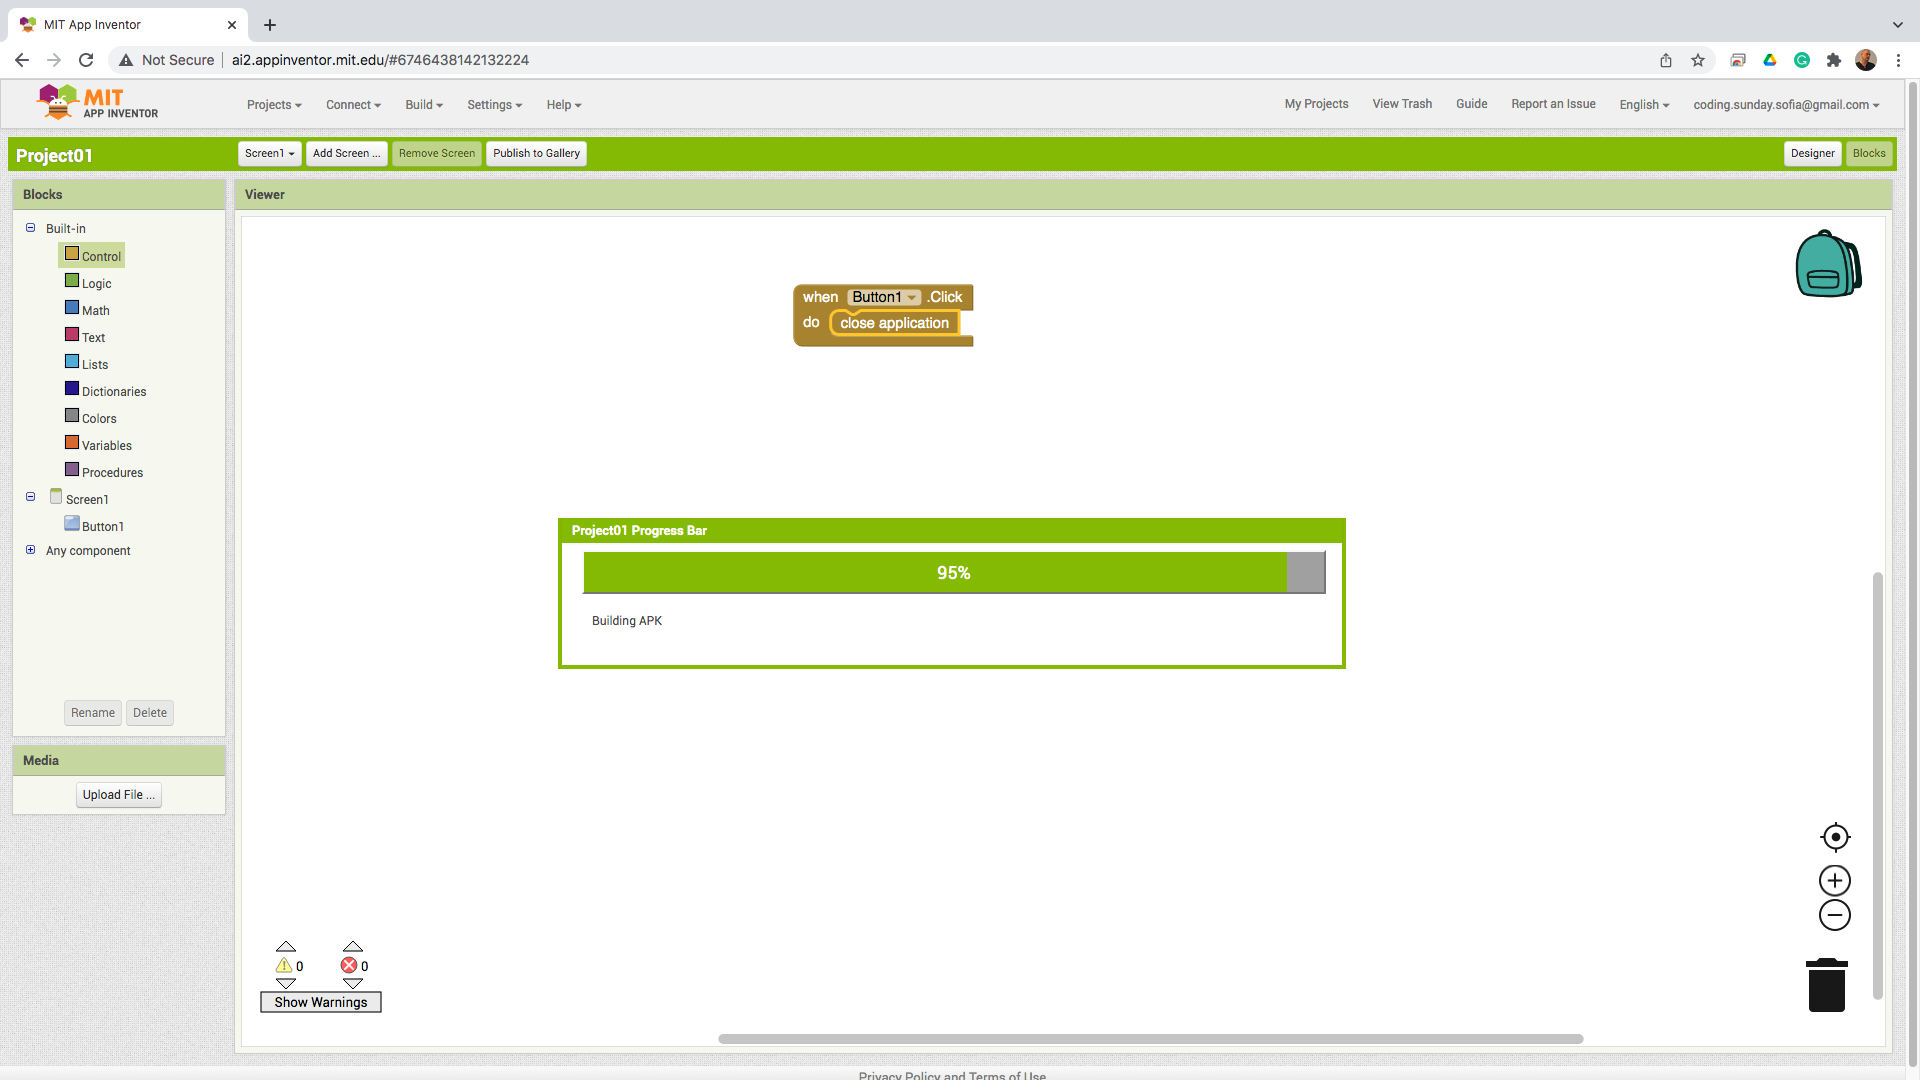
\includegraphics[width=1.0\linewidth,height=0.5\linewidth]{fig010039.png}
   \caption{App build progress}
\label{fig010039}
\end{figure}

After the project is compiled and the installation package is created, the programming environment offers a QR code (Fig. \ref{fig010040}) through which the installation package can be downloaded from the mobile device (phone or tablet).

\begin{figure}[H]
   \centering
   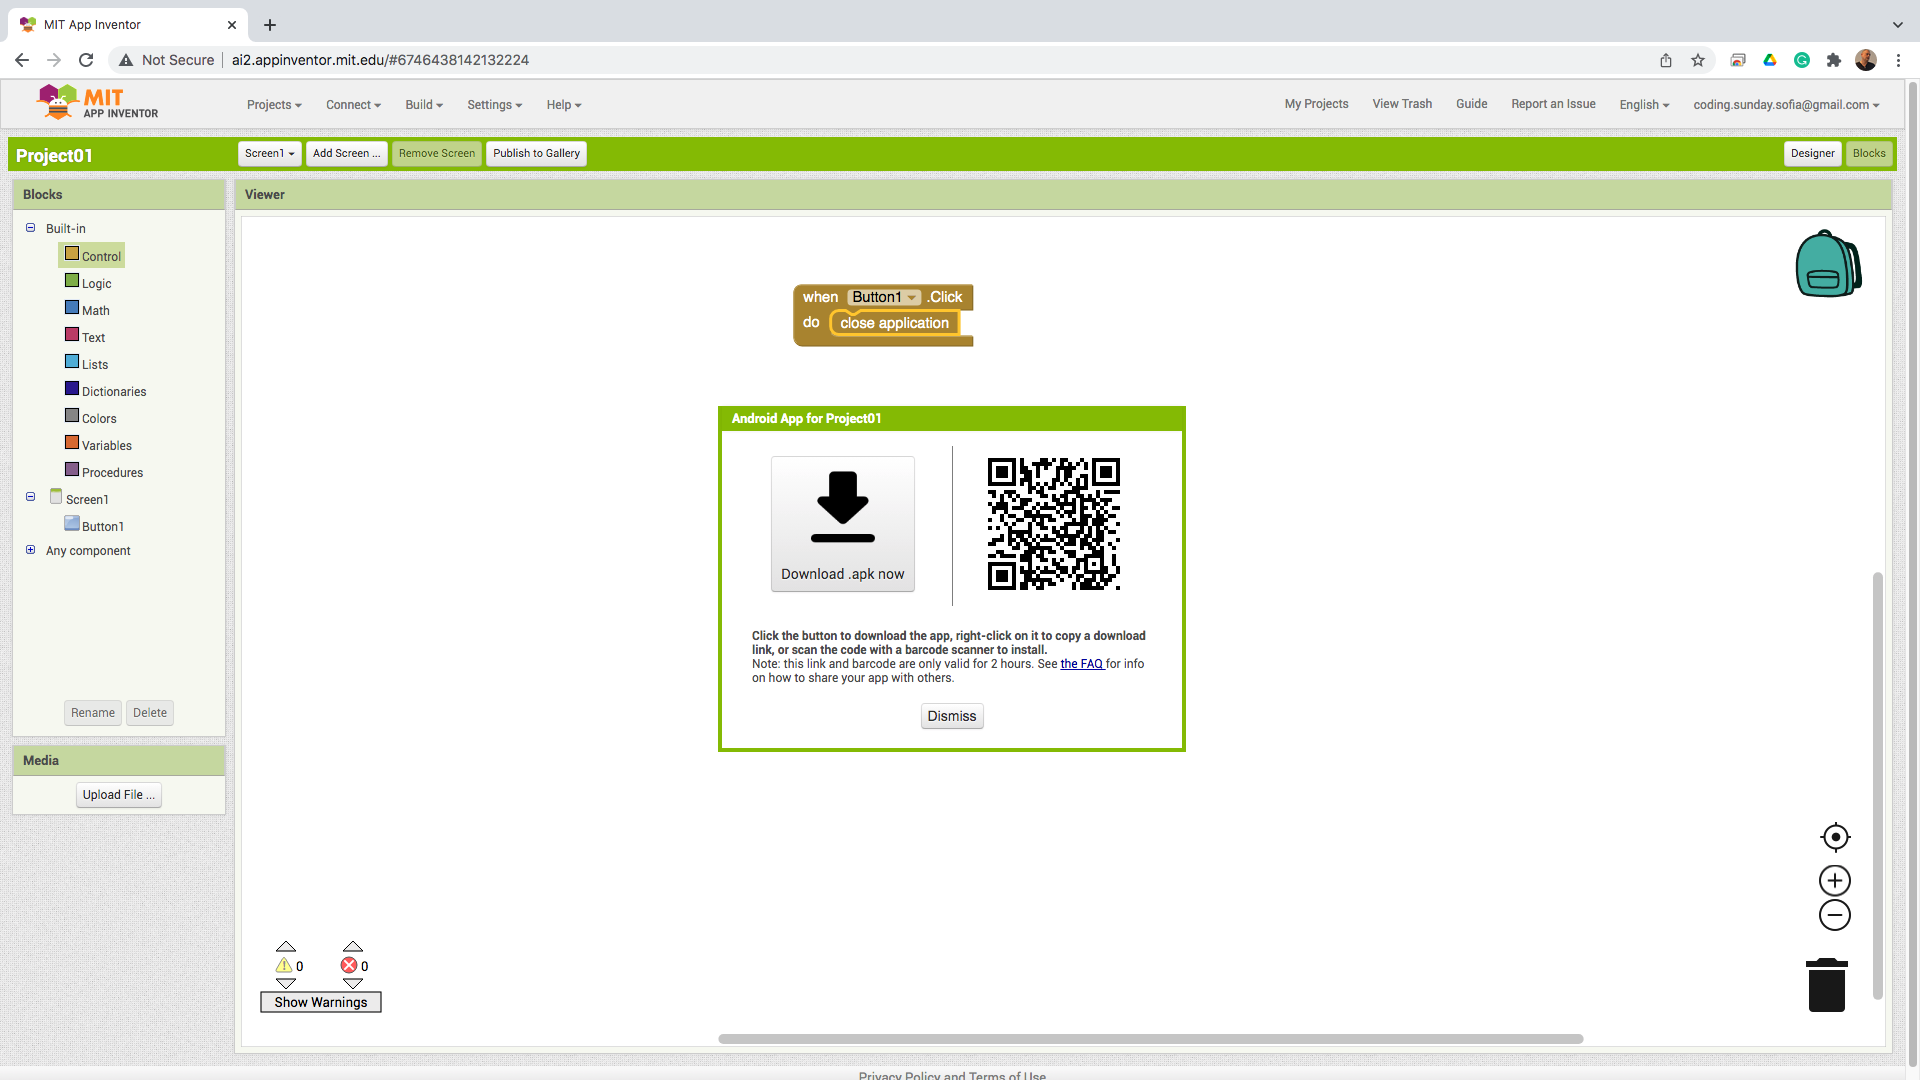
\includegraphics[width=1.0\linewidth,height=0.5\linewidth]{fig010040.png}
   \caption{Code for installing the application on a mobile device}
\label{fig010040}
\end{figure}

The creators of the App Inventor programming environment have foreseen the possibility of a faster and easier installation of the written programs through a specially created application (MIT AI2 Companion), which will take over the communication with the cloud infrastructure of App Inventor (Fig. \ref{fig010041}). The application is available on Google Play and requires no special skills to be installed on a personal mobile device.

\begin{figure}[H]
   \centering
   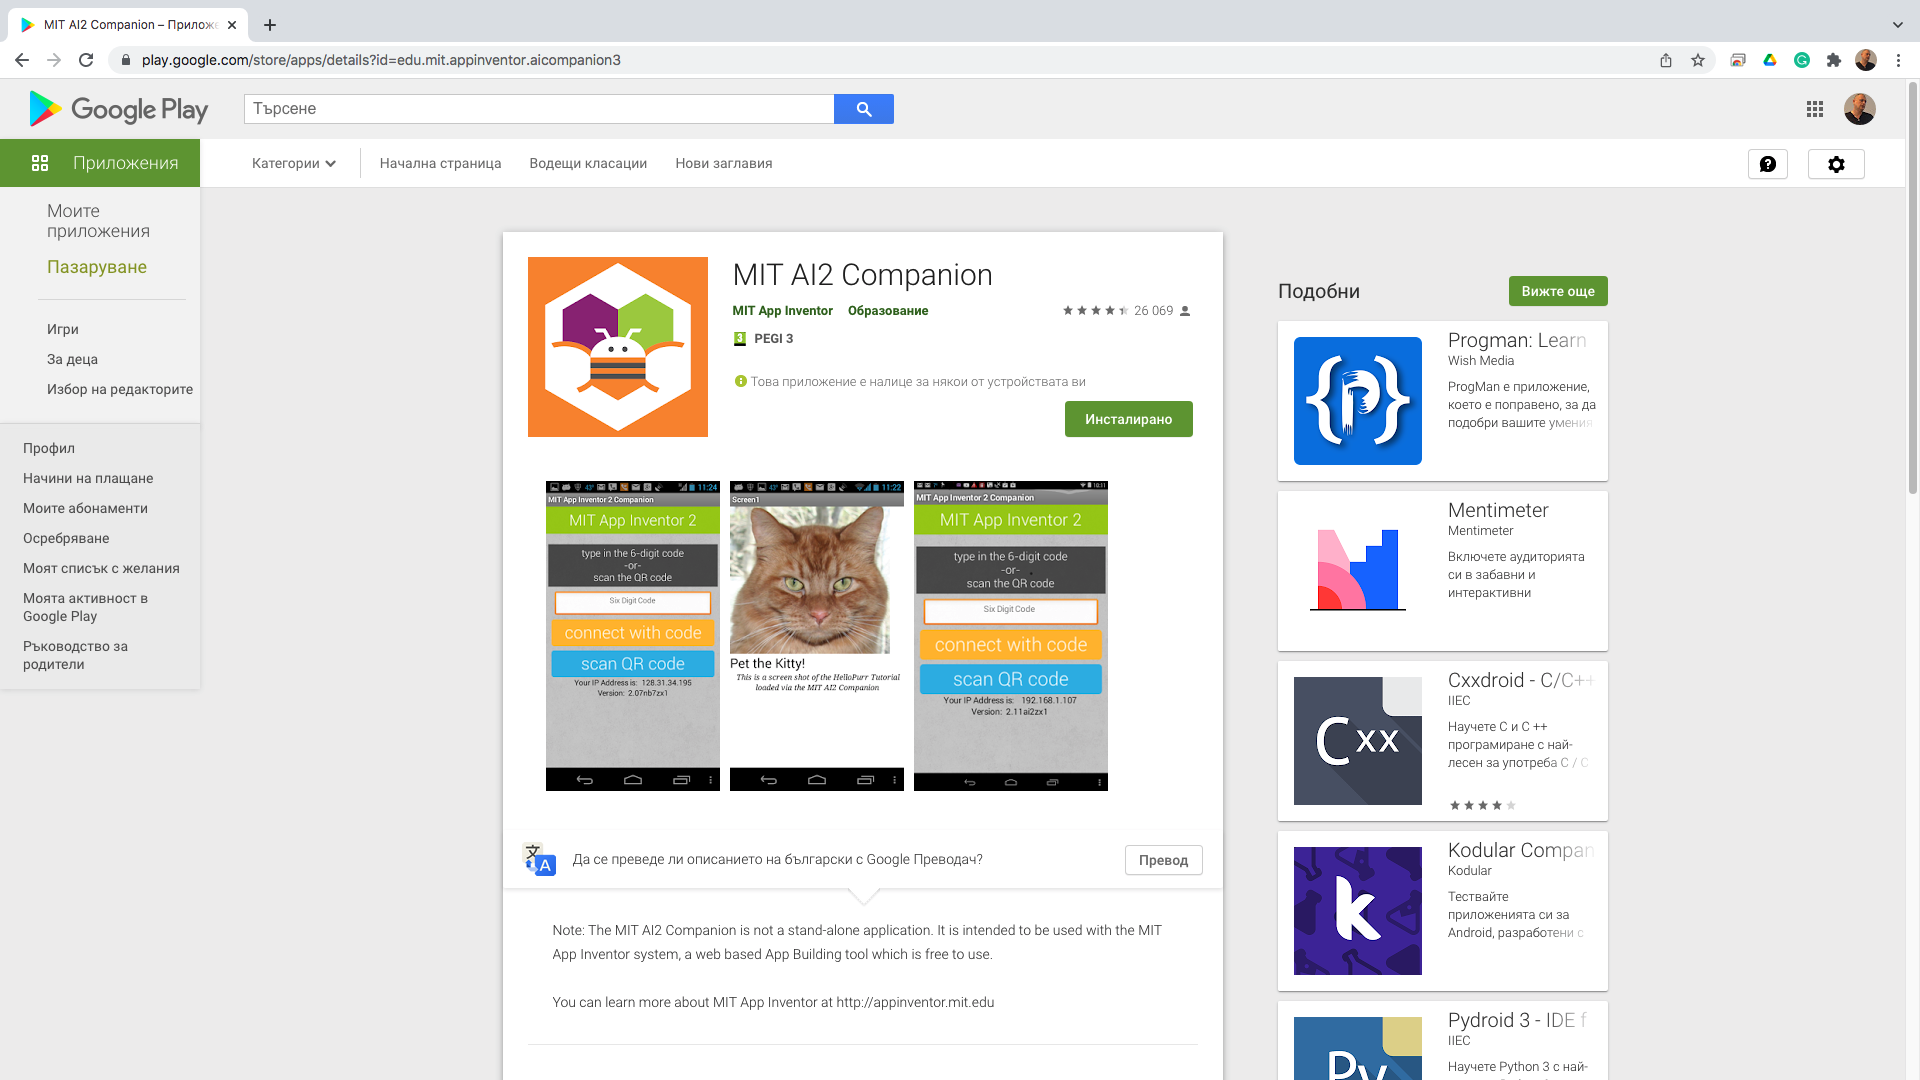
\includegraphics[width=1.0\linewidth,height=0.5\linewidth]{fig010041.png}
   \caption{Mobile application for managing compiled projects}
\label{fig010041}
\end{figure}

When the MIT AI2 Companion is started, the application gives two options to download the already written programs (Fig. \ref{fig010042}). One option is entering a code, and the second is scanning a QR code. Scanning the QR code is significantly faster and more convenient (Fig. \ref{fig010043}). Since the installation package is an executable file, the Android operating system warns that such files may be dangerous (Fig. \ref{fig010044}).

\begin{figure}[H]
   \begin{subfigure}{0.31\textwidth}
   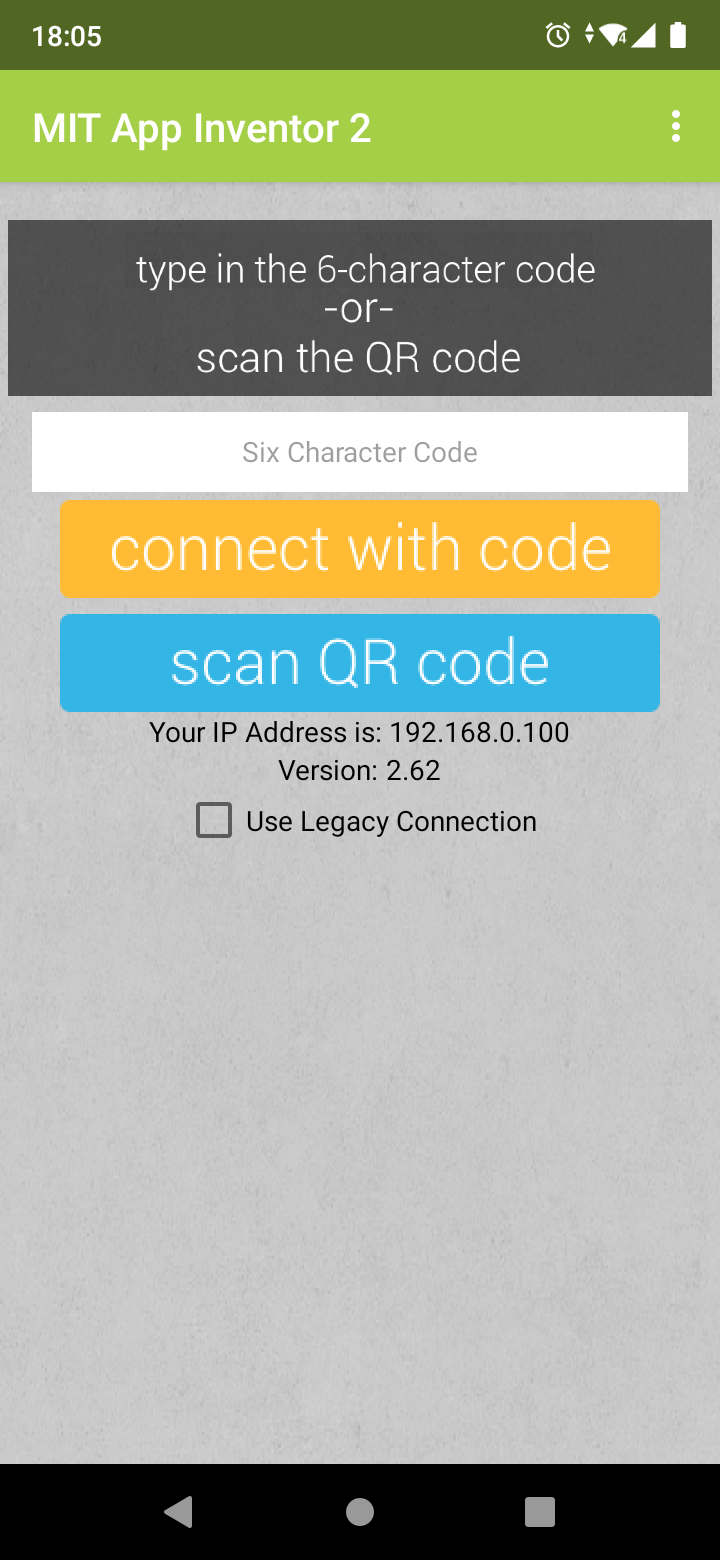
\includegraphics[width=\linewidth]{fig010042.png}
   \subcaption{\tiny Installation Selection}
   \label{fig010042}
   \end{subfigure}
   \begin{subfigure}{0.31\textwidth}
   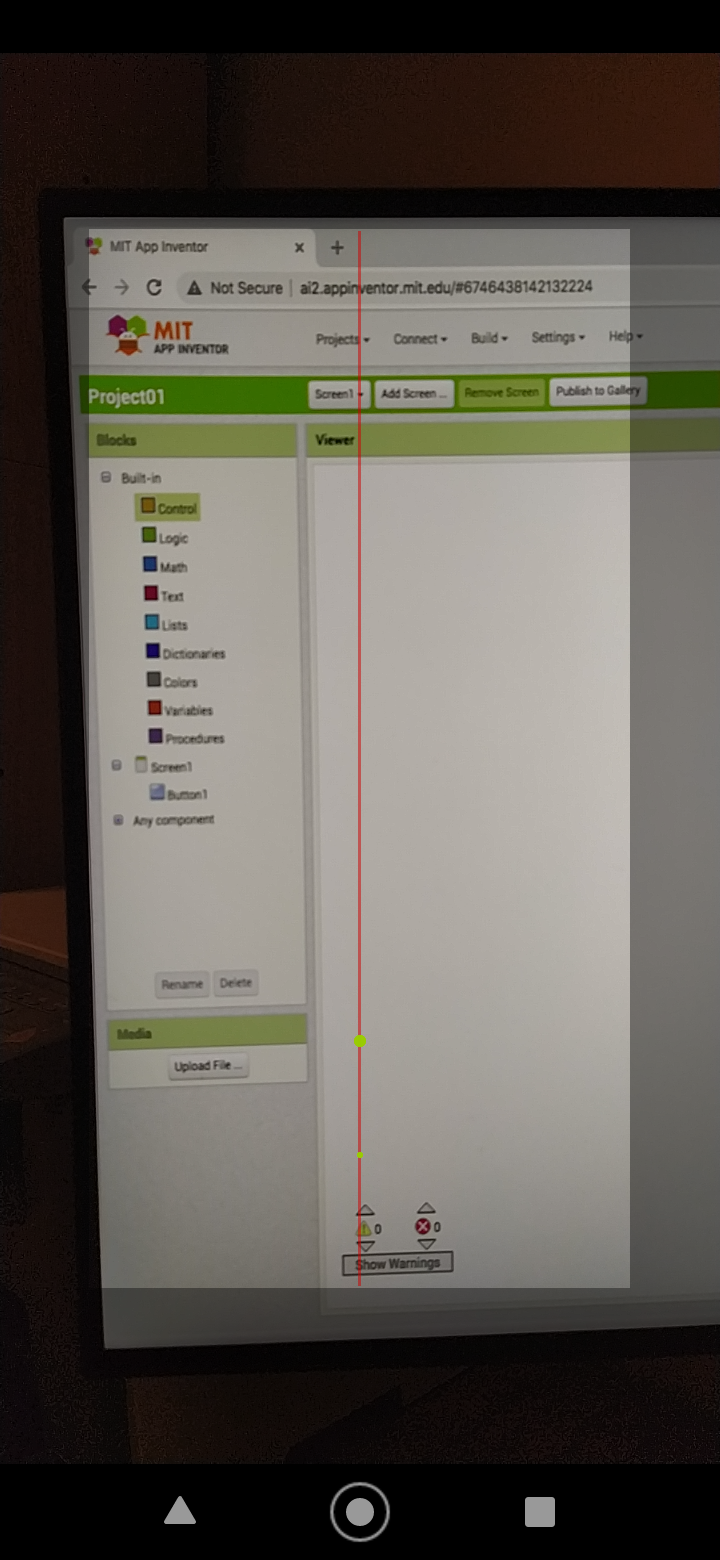
\includegraphics[width=\linewidth]{fig010043.png}
   \subcaption{\tiny Code Scan}
   \label{fig010043}
   \end{subfigure}
   \begin{subfigure}{0.31\textwidth}
   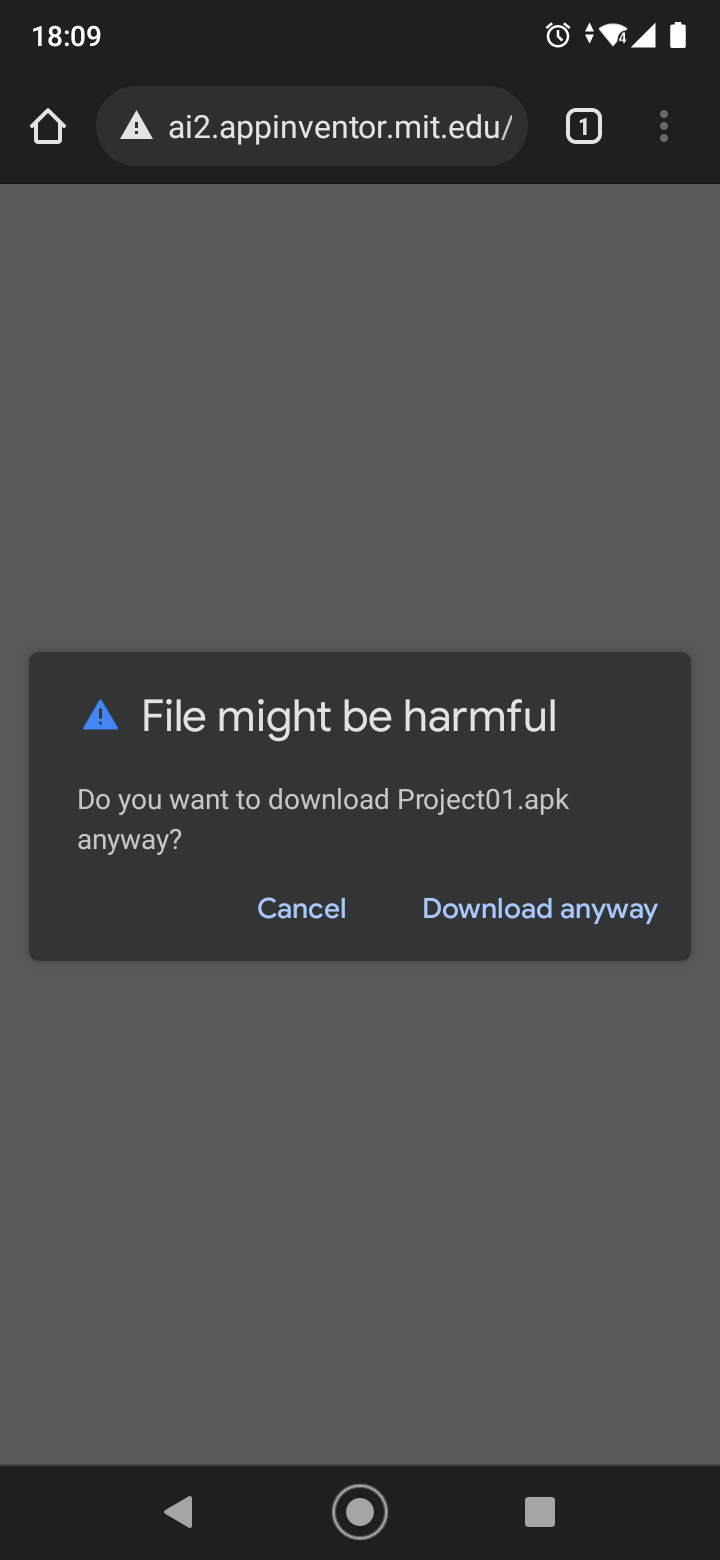
\includegraphics[width=\linewidth]{fig010044.png}
   \subcaption{\tiny Download File}
   \label{fig010044}
   \end{subfigure}
   \caption{Install via QR code}
\end{figure}

After downloading the installation package, the operating system issues a message about the successful operation of recording the installer (Fig. \ref{fig010045}). The user must select the installation package and activate it. This prompts you to ask if you want to install the program in the downloaded file (Fig. \ref{fig010046}). Although we know exactly how the installation file was created, the operating system perceives it as a program developed by an unverified developer. For this reason, it asks the user again if he wants to do the installation (Fig. \ref{fig010047}).

\begin{figure}[H]
   \begin{subfigure}{0.31\textwidth}
   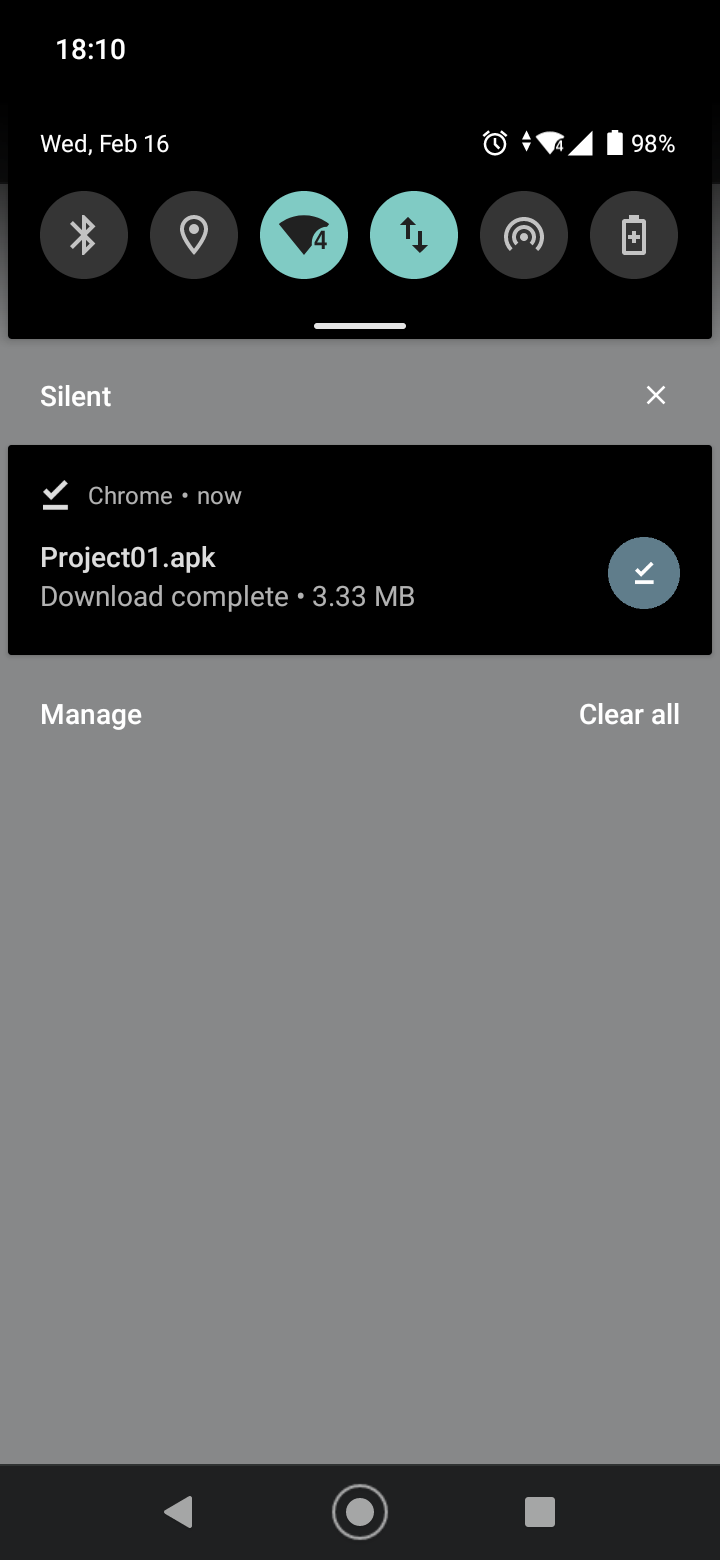
\includegraphics[width=\linewidth]{fig010045.png}
   \subcaption{\tiny File Downloaded}
   \label{fig010045}
   \end{subfigure}
   \begin{subfigure}{0.31\textwidth}
   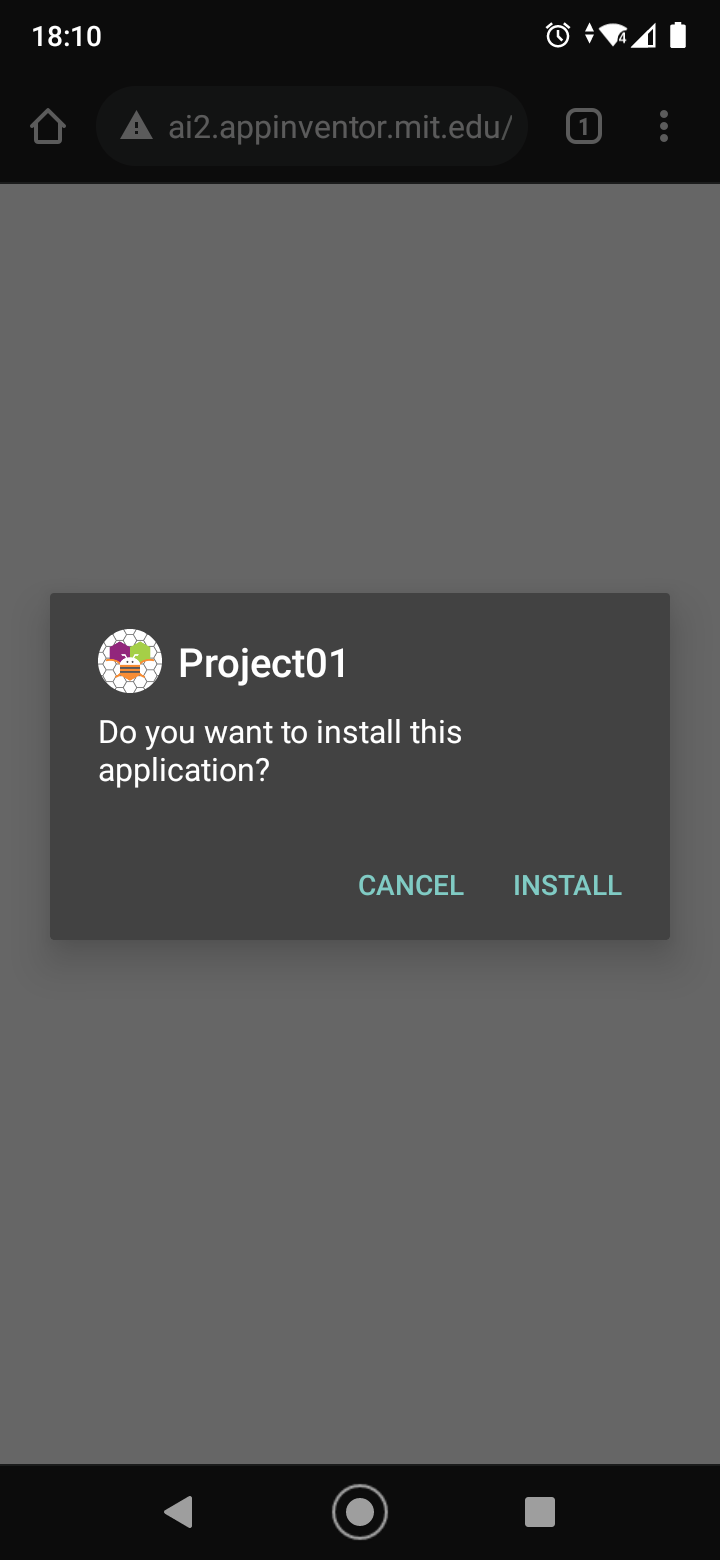
\includegraphics[width=\linewidth]{fig010046.png}
   \subcaption{\tiny Choose to install}
   \label{fig010046}
   \end{subfigure}
   \begin{subfigure}{0.31\textwidth}
   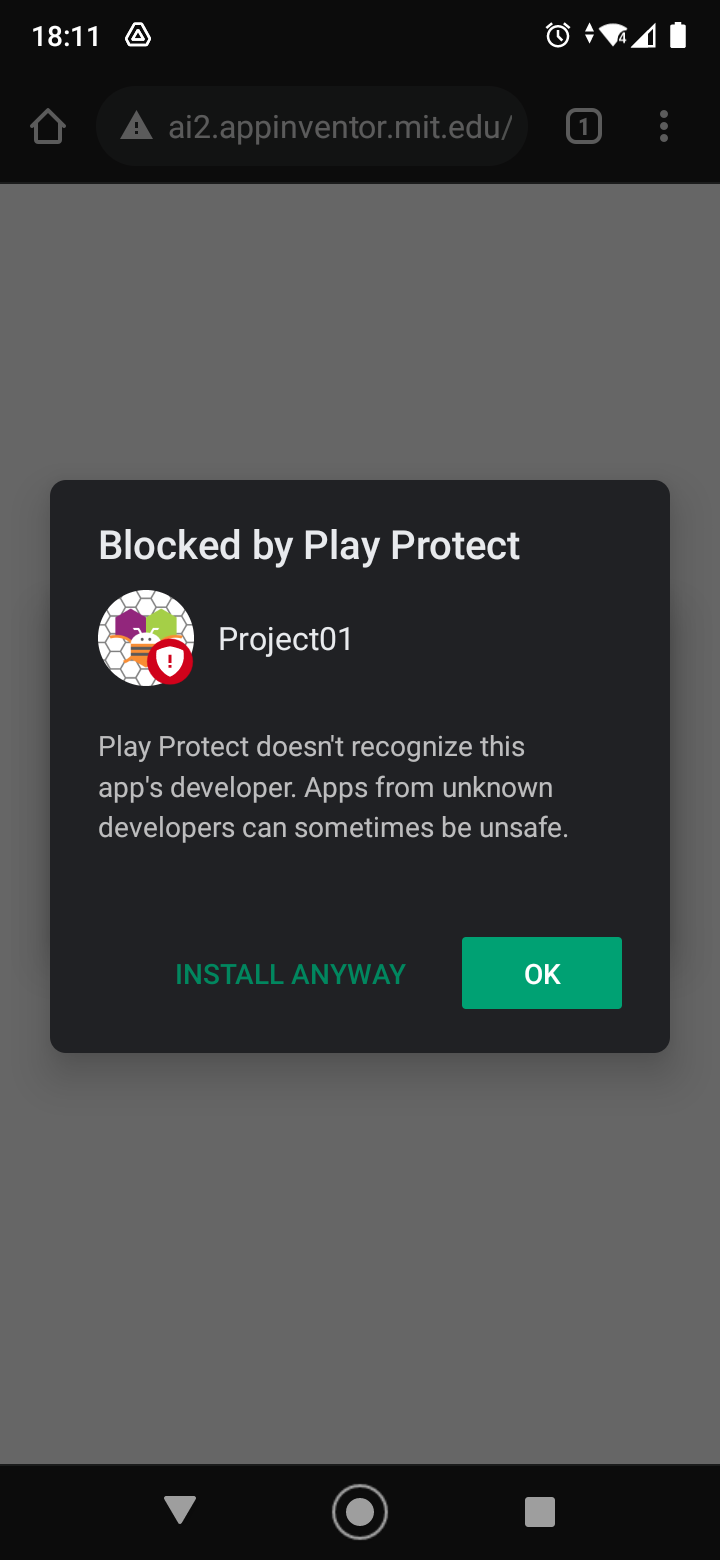
\includegraphics[width=\linewidth]{fig010047.png}
   \subcaption{\tiny Installation Confirmation}
   \label{fig010047}
   \end{subfigure}
   \caption{Installation on the mobile device}
\end{figure}

"Install Anyway" is selected, and the written program is installed on the mobile device. The installation process ends with a window prompting to start the newly installed program (Fig. \ref{fig010048}). To check the operation of the written code, it is enough to press the visualized button in the upper left corner (Fig. \ref{fig010049}). This action results in closing the window and visualizing the virtual wallpaper (Fig. \ref{fig010049}).

\begin{figure}[H]
   \begin{subfigure}{0.31\textwidth}
   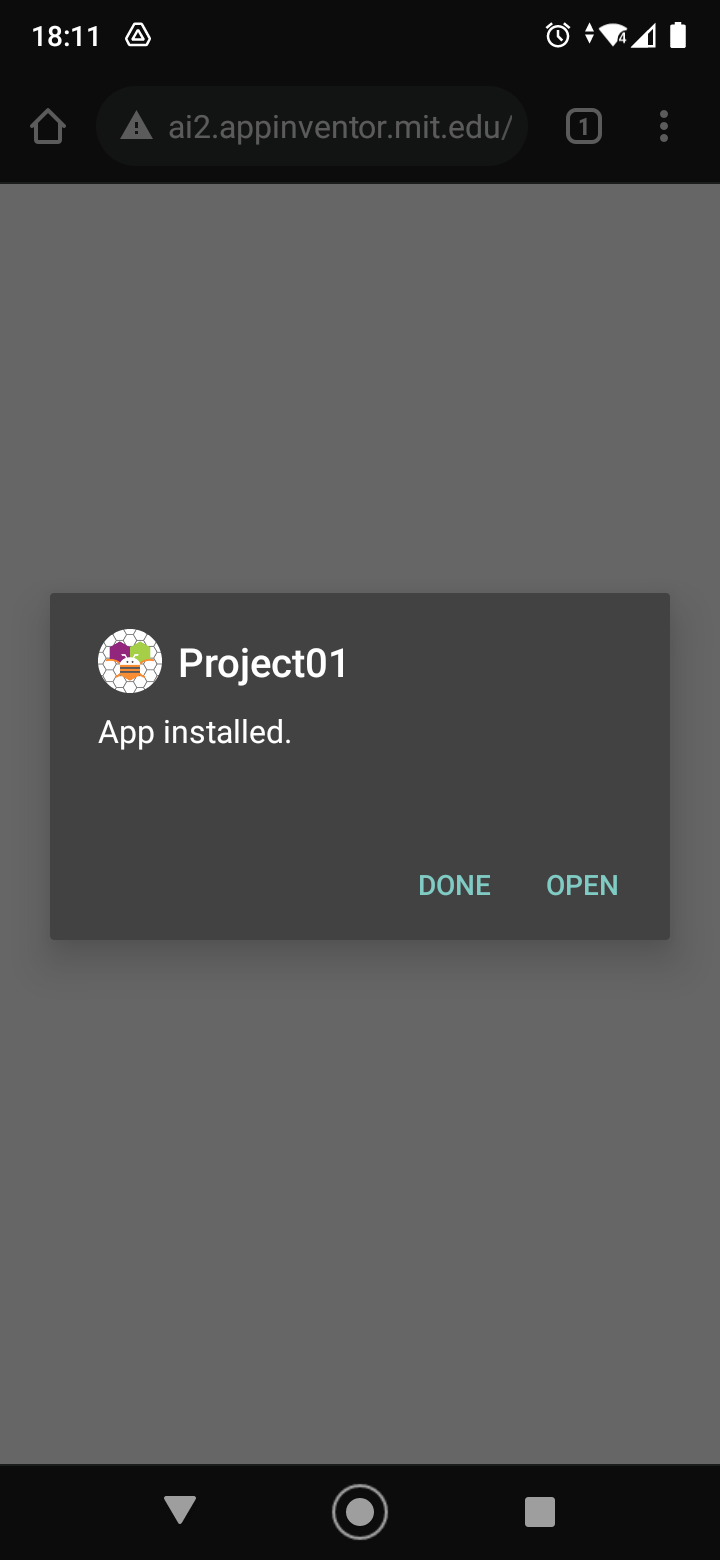
\includegraphics[width=\linewidth]{fig010048.png}
   \subcaption{\tiny Launch}
   \label{fig010048}
   \end{subfigure}
   \begin{subfigure}{0.31\textwidth}
   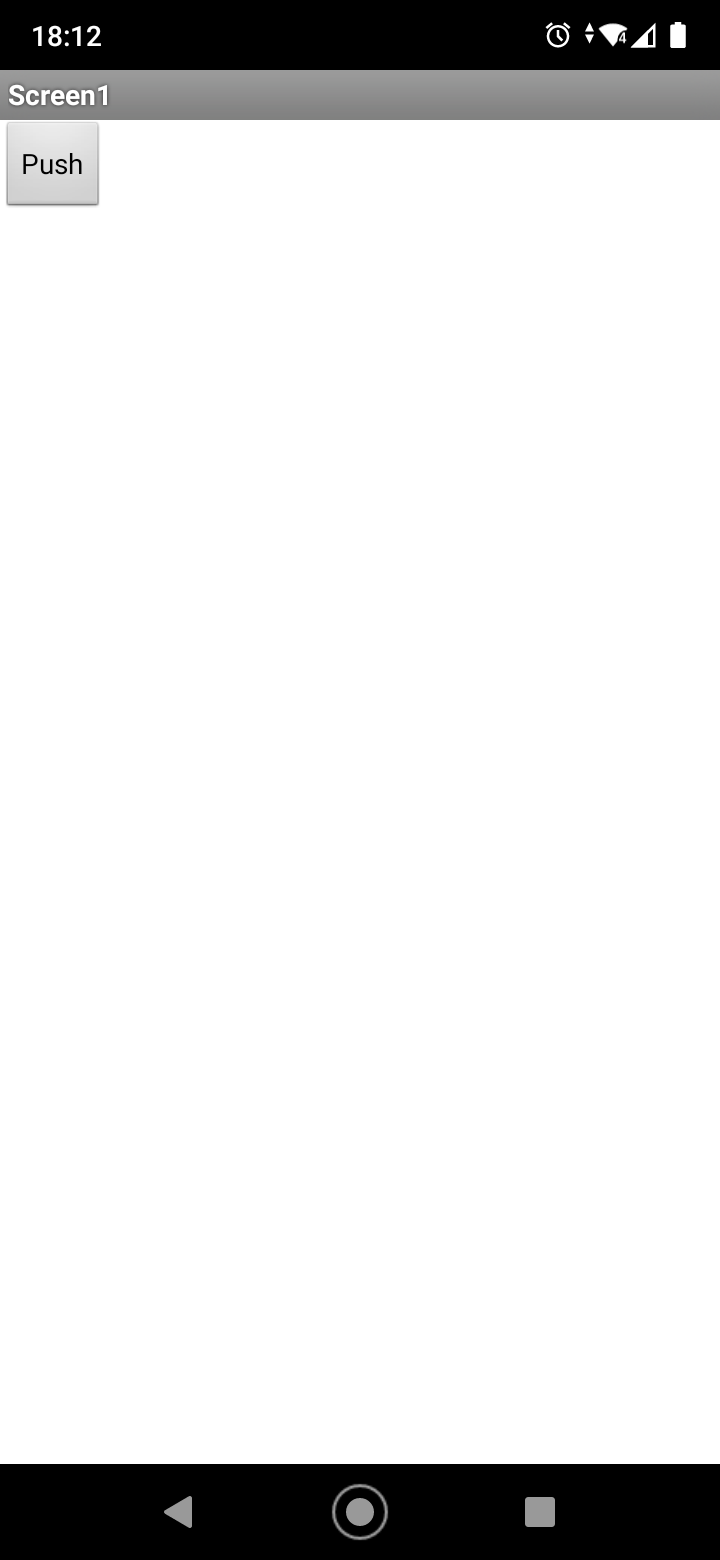
\includegraphics[width=\linewidth]{fig010049.png}
   \subcaption{\tiny Button Selection}
   \label{fig010049}
   \end{subfigure}
   \begin{subfigure}{0.31\textwidth}
   \includegraphics[width=\linewidth]{fig010050.png}
   \subcaption{\tiny Closed App}
   \label{fig010050}
   \end{subfigure}
   \caption{Working with the application}
\end{figure}

With App Inventor, the most fascinating part is that the developed programs become available on mobile devices, and the person who creates them can show their work even when they are not in front of the computer or do not have Internet connectivity.
\newpage
\chapter{Programming Constructs}

Computer programs are made up of a strict sequence of instructions. Such sequences are called an algorithm. We, humans, run various algorithms every day as part of our daily lives. Getting ready and going to school is an algorithm. We wake up, get dressed, do our morning outfit, have breakfast, leave the house, and move to school. A very vivid example of an algorithm is cooking recipes. There are starting products in a recipe, then precise instructions on how to process and mix the products, with a clear idea of the end result. In computer programs, a basic set of instructions make up the means of expression of the corresponding programming language. The charm of block languages is that this basic set of instructions is represented visually in the form of colored blocks. The arrangement of the colored blocks in a strictly defined sequence leads to the creation of small computer programs.

In the case of Scratch, the program has well-defined start and end points. With App Inventor, the approach is slightly different. There, the sequence of instructions that make up the written program is entered in small fragments called events. Events are triggered by various user or operating system actions. In Scratch, we talk about sequential programming; in App Inventor, we talk about event programming. The basic programming constructs in the two programming environments are identical, but there are also some significant differences. To write efficient and reliable programs, knowing the means of expression of our programming environments is essential. 

\section{Programming Constructs in Scratch}

The basic building blocks in Scratch are organized into colored groups (Fig. \ref{fig020001}). This organization helps to navigate faster and use the different blocks more efficiently.

\begin{figure}[H]
   \centering
   \includegraphics[width=1.0\linewidth,height=0.5\linewidth]{fig020001.png}
   \caption{Grouping instructions}
\label{fig020001}
\end{figure}

The most significant block in the program is the block that initiates the execution of the instructions arranged below it. This block has a green flag (Fig. \ref{fig020002}) and defines what will happen after the program is started.

\begin{figure}[H]
   \centering
   \includegraphics[width=1.0\linewidth,height=0.5\linewidth]{fig020002.png}
   \caption{Starting point of the program}
\label{fig020002}
\end{figure}

The program launch block is in the light orange group, designed to react to user events. The exact moment the user wants the program to start its execution is undefined in time, so Scratch must catch an event triggered by the user himself.

The second most significant block ends the program (Fig. \ref{fig020003}). It is located in the dark orange group and has the task of stopping all processes taking place during the execution of the program itself.

\begin{figure}[H]
   \centering
   \includegraphics[width=1.0\linewidth,height=0.5\linewidth]{fig020003.png}
   \caption{Program endpoint}
\label{fig020003}
\end{figure}

The dark orange group contains performance control blocks. These blocks allow the program to take different paths and a group of actions to be repeated many times.

In Scratch, instruction blocks basically control pictures called sprites. Unlike an ordinary computer image, a sprite is a graphic object containing multiple frames showing the character's image in different configurations. Every new Scratch program starts with a single sprite of the orange cat, located at coordinates (x=0,y=0). The workspace is a two-dimensional coordinate system centered at (0,0).

\begin{figure}[H]
   \centering
   \includegraphics[width=1.0\linewidth,height=0.5\linewidth]{fig020004.png}
   \caption{Finish immediately after starting}
\label{fig020004}
\end{figure}

The program does nothing if the start and end blocks are joined (Fig. \ref{fig020004}). Practically, this program ends as soon as it starts. A program that does nothing is entirely pointless. To start something happening, use the blocks in the blue group. The first block instructs the kitten to move 10 steps, and the number of steps can be changed by writing another number inside the block (Fig. \ref{fig020005}).

\begin{figure}[H]
   \centering
   \includegraphics[width=1.0\linewidth,height=0.5\linewidth]{fig020005.png}
   \caption{Moving character}
\label{fig020005}
\end{figure}

The next block in the group instructs the character to rotate a specified number of degrees, clockwise, relative to its own center (Fig. \ref{fig020006}).

\begin{figure}[H]
   \centering
   \includegraphics[width=1.0\linewidth,height=0.5\linewidth]{fig020006.png}
   \caption{Clockwise Rotation}
\label{fig020006}
\end{figure}

Similarly, with the next block in the group, the rotation can be performed counterclockwise (Fig. \ref{fig020007}).

\begin{figure}[H]
   \centering
   \includegraphics[width=1.0\linewidth,height=0.5\linewidth]{fig020007.png}
   \caption{Counterclockwise Rotation}
\label{fig020007}
\end{figure}

The next block in the group allows the character to move to random coordinates or coordinates specified with the mouse (Fig. \ref{fig020008}).

\begin{figure}[H]
   \centering
   \includegraphics[width=1.0\linewidth,height=0.5\linewidth]{fig020008.png}
   \caption{Move to random position}
\label{fig020008}
\end{figure}

The character's movement can also be set by absolute coordinates with a block allowing entering numbers for the abscissa and ordinate axis (Fig. \ref{fig020009}).

\begin{figure}[H]
   \centering
   \includegraphics[width=1.0\linewidth,height=0.5\linewidth]{fig020009.png}
   \caption{Move by absolute coordinates}
\label{fig020009}
\end{figure}

Smooth movement at a predetermined time interval is possible at random coordinates or coordinates specified with the mouse, thanks to the next block in the group (Fig. \ref{fig020010}).

\begin{figure}[H]
   \centering
   \includegraphics[width=1.0\linewidth,height=0.5\linewidth]{fig020010.png}
   \caption{Slide to random position}
\label{fig020010}
\end{figure}

Smooth sliding to predetermined coordinates for a predetermined time interval is possible with the block designed for this purpose (Fig. \ref{fig020011}).

\begin{figure}[H]
   \centering
   \includegraphics[width=1.0\linewidth,height=0.5\linewidth]{fig020011.png}
   \caption{Slide to set coordinates}
\label{fig020011}
\end{figure}

The animated character has an orientation property in the form of an angle. At 90 degrees, the orange cat is looking to the right. To change the character's orientation, a block with the possibility of entering a specific angle is used (Fig. \ref{fig020012}).

\begin{figure}[H]
   \centering
   \includegraphics[width=1.0\linewidth,height=0.5\linewidth]{fig020012.png}
   \caption{Corner Orientation}
\label{fig020012}
\end{figure}

In more complex character control scenarios, sometimes the character needs to follow the mouse pointer. For this purpose, a specific block executes this instruction (Fig. \ref{fig020013}).

\begin{figure}[H]
   \centering
   \includegraphics[width=1.0\linewidth,height=0.5\linewidth]{fig020013.png}
   \caption{Mouse Pointer Orientation}
\label{fig020013}
\end{figure}

Blocks can be placed one after the other, and for sequential change of the relative x and y coordinates (relative to the current position) of the character, there are specially defined blocks (Fig. \ref{fig020014}).

\begin{figure}[H]
   \centering
   \includegraphics[width=1.0\linewidth,height=0.5\linewidth]{fig020014.png}
   \caption{Sequential change of relative coordinates}
\label{fig020014}
\end{figure}

In addition to a relative change of the coordinates, an absolute change of the coordinates is also possible, with the absolute change relative to the center of the coordinate system (Fig. \ref{fig020015}).

\begin{figure}[H]
   \centering
   \includegraphics[width=1.0\linewidth,height=0.5\linewidth]{fig020015.png}
   \caption{Sequential change of absolute coordinates}
\label{fig020015}
\end{figure}

In its movement, when the animated character reaches the boundaries of the workspace, one option is to continue the movement outside the visible area. The other option is to take action and have the character bounce off the edges of the workspace. There is a specific block for this bounce (Fig. \ref{fig020016}). A slightly more complicated sequence of instructions is needed to illustrate its operation. Each time the program is run. First, the relative coordinates are changed, and then an edge bounce is performed if necessary. To make the verification scenario a bit more interesting, instead of fixed relative offset values, an embedding of one of the green blocks are used, allowing for the generation of a random number within a predetermined range. It is important to note that the green block has an oval shape, which suggests it is intended to fit into one of the other blocks with an oval slot.

\begin{figure}[H]
   \centering
   \includegraphics[width=1.0\linewidth,height=0.5\linewidth]{fig020016.png}
   \caption{Bouncing off the edges}
\label{fig020016}
\end{figure}

Next, a handy block from the group of dark orange is the block for waiting a period (Fig. \ref{fig020017}). When this block is placed between the start and end blocks, the program waits the specified number of seconds before stopping execution. During execution, it can be clearly observed that a yellow frame appears around the sequence of instructions, which symbolizes the mode of executing instructions.

\begin{figure}[H]
   \centering
   \includegraphics[width=1.0\linewidth,height=0.5\linewidth]{fig020017.png}
   \caption{Wait instruction}
\label{fig020017}
\end{figure}

The group of purple blocks contains instructions for the outer layout of the animated character. The first two blocks are intended for lines (Fig. \ref{fig020018}) that the character says (spelled as in a comic book). The first block sets the text on the screen until the next instruction. This is precisely why there needs to be a few seconds of waiting so the text remains visible to the user. The second block also has a parameter to determine how many seconds the text should be visible to the user.

\begin{figure}[H]
   \centering
   \includegraphics[width=1.0\linewidth,height=0.5\linewidth]{fig020018.png}
   \caption{Writing cues to speak}
\label{fig020018}
\end{figure}

The second two blocks are intended for lines the animated character thinks but does not say. The difference is in how the text is visualized (Fig. \ref{fig020019}).

\begin{figure}[H]
   \centering
   \includegraphics[width=1.0\linewidth,height=0.5\linewidth]{fig020019.png}
   \caption{Writing lines, as a thought}
\label{fig020019}
\end{figure}

Animated characters in Scratch are in the form of sprites. A sprite is a set of images of the character in different poses. Two blocks are used to change these different poses (Fig. \ref{fig020020}). The first set is a specific frame in the sprite, and the second is the next frame in the sequence.

\begin{figure}[H]
   \centering
   \includegraphics[width=1.0\linewidth,height=0.5\linewidth]{fig020020.png}
   \caption{Changing Poses}
\label{fig020020}
\end{figure}

In addition to the animated characters (sprites), the work scene has a background image. This background image is also subject to change, for which two separate blocks are provided (Fig. \ref{fig020021}). With the first one, background images can be selected forward, backward, randomly, or with a specific name, and with the second block, the next image in the sequence.

\begin{figure}[H]
   \centering
   \includegraphics[width=1.0\linewidth,height=0.5\linewidth]{fig020021.png}
   \caption{Change background}
\label{fig020021}
\end{figure}

There are two specific blocks for resizing the animated character, the first resizing in absolute values and the second resizing in percentages relative to the original size (Fig. \ref{fig020022}).

\begin{figure}[H]
   \centering
   \includegraphics[width=1.0\linewidth,height=0.5\linewidth]{fig020022.png}
   \caption{Resize}
\label{fig020022}
\end{figure}

Three blocks are provided for changing the visual layout of the animated character (Fig. \ref{fig020023}). The first two set a change, which can be in color, various distortions, pixelation, mosaic, transparency, or brightness, and the third block cancels any decorations made. The first block causes a relative change to the character's current state, and the second block sets a fundamental change. Again, giving it a few seconds is essential so that the changes are clearly discernible.

\begin{figure}[H]
   \centering
   \includegraphics[width=1.0\linewidth,height=0.5\linewidth]{fig020023.png}
   \caption{Change appearance}
\label{fig020023}
\end{figure}

Working with sprites is primarily for achieving animated effects. The different animated characters in the scene have specific interactions with each other. The script of the developed project determines at what moment each of the characters appears on the scene and at what moment they disappear. Two blocks performing these actions are provided to carry out the appearance and disappearance (Fig. \ref{fig020024}).

\begin{figure}[H]
   \centering
   \includegraphics[width=1.0\linewidth,height=0.5\linewidth]{fig020024.png}
   \caption{Hide and show}
\label{fig020024}
\end{figure}

Many bitmap software products organize different images into layers. Examples are Adobe Photoshop, GIMP, Microsoft Word, and LibreOffice Draw. The layered organization is logical, as different sprites can overlap at specific points in time. In some of the graphics software packages, layers are perceived as a Z-buffer. In Scratch, the ability to work with layers is also available, with two specific blocks allowing the sprite to move forward and backward through the layers (Fig. \ref{fig020025}).

\begin{figure}[H]
   \centering
   \includegraphics[width=1.0\linewidth,height=0.5\linewidth]{fig020025.png}
   \caption{Navigation through layers}
\label{fig020025}
\end{figure}

The group of blocks in magenta is for sound layout. The performance of sounds is achieved with the first two blocks in the group (Fig. \ref{fig020026}). The first block plays the sound until it is finished, and the second block starts it and passes the playback to the next block. With the third block, all playing sounds are stopped. The software environment also allows sounds to be recorded from the user's computer.

\begin{figure}[H]
   \centering
   \includegraphics[width=1.0\linewidth,height=0.5\linewidth]{fig020026.png}
   \caption{Playing Sounds}
\label{fig020026}
\end{figure}

The pitch (frequency) and stereo (left/right) blocks can change two of the sounds' characteristics. Both blocks have numerical values for the specified characteristics (Fig. \ref{fig020027}).

\begin{figure}[H]
   \centering
   \includegraphics[width=1.0\linewidth,height=0.5\linewidth]{fig020027.png}
   \caption{Sound Characteristics}
\label{fig020027}
\end{figure}

To achieve a richer sound picture, the strength of the different sounds can be controlled with two blocks (Fig. \ref{fig020028}). The former controls volume in absolute value, the latter as percentages.

\begin{figure}[H]
   \centering
   \includegraphics[width=1.0\linewidth,height=0.5\linewidth]{fig020028.png}
   \caption{Volume}
\label{fig020028}
\end{figure}

The orange group of blocks is for events to occur. Events are a tool for executing instructions when there is no explicit cutoff for when program instructions must be performed. Such an event is pressing a button on the keyboard by the user (Fig. \ref{fig020029}).

\begin{figure}[H]
   \centering
   \includegraphics[width=1.0\linewidth,height=0.5\linewidth]{fig020029.png}
   \caption{Key Press Event}
\label{fig020029}
\end{figure}

Mouse clicking on a specific sprite can also be handled using a suitable block (Fig. \ref{fig020030}).

\begin{figure}[H]
   \centering
   \includegraphics[width=1.0\linewidth,height=0.5\linewidth]{fig020030.png}
   \caption{Mouse Click Event}
\label{fig020030}
\end{figure}

Changing the background can also trigger an event to be handled. A block is provided for this purpose (Fig. \ref{fig020031}).

\begin{figure}[H]
   \centering
   \includegraphics[width=1.0\linewidth,height=0.5\linewidth]{fig020031.png}
   \caption{BackgroundChange Event}
\label{fig020031}
\end{figure}

An event can be caught after a particular time has elapsed to a timer or a certain sound level has been reached (Fig. \ref{fig020032}).

\begin{figure}[H]
   \centering
   \includegraphics[width=1.0\linewidth,height=0.5\linewidth]{fig020032.png}
   \caption{Timer or sound event}
\label{fig020032}
\end{figure}

Event handling is also associated with a mechanism for sending/receiving messages. One block of instructions can broadcast a predefined message, and another can subscribe to receive precisely that kind of message (Fig. \ref{fig020033}).

\begin{figure}[H]
   \centering
   \includegraphics[width=1.0\linewidth,height=0.5\linewidth]{fig020033.png}
   \caption{Broadcasting and receiving messages}
\label{fig020033}
\end{figure}

Since working with the messaging engine may require synchronization, it has a separate block that propagates the message and waits for actions to be taken on its interception (Fig. \ref{fig020034}). The programmer can create different messages to be sent in different situations.

\begin{figure}[H]
   \centering
   \includegraphics[width=1.0\linewidth,height=0.5\linewidth]{fig020034.png}
   \caption{Propagating a pending message}
\label{fig020034}
\end{figure}

The most essential and valuable blocks are organized in the dark orange group. These blocks define which execution path to take, given the possible choices for executing instructions. When the desire is to perform a specific action repeatedly, with a set number of repetitions, there is a particular block for this purpose (Fig. \ref{fig020035}). Multiple iterations are accomplished in programming using loop constructs, as with this iteration block.

\begin{figure}[H]
   \centering
   \includegraphics[width=1.0\linewidth,height=0.5\linewidth]{fig020035.png}
   \caption{Fixed number of iterations}
\label{fig020035}
\end{figure}

The word repeat in English means repeat. The number in the pad determines how many repetitions to execute, and the slot in the pad is where the instructions to be repeated are placed. In this example, the kitten is moved to randomly selected coordinates, followed by a predetermined number of seconds to wait. In infrequent situations, there is a need for an infinitely repeating loop, for which a separate block is provided (Fig. \ref{fig020036}).

\begin{figure}[H]
   \centering
   \includegraphics[width=1.0\linewidth,height=0.5\linewidth]{fig020036.png}
   \caption{Infinite Replays}
\label{fig020036}
\end{figure}

The next block is one of the most essential blocks in programming. It is called a conditional execution block (Fig. \ref{fig020037}) or a conditional transition. The block's content is executed only if the condition in its header is fulfilled.

\begin{figure}[H]
   \centering
   \includegraphics[width=1.0\linewidth,height=0.5\linewidth]{fig020037.png}
   \caption{Execution on condition}
\label{fig020037}
\end{figure}

This dark orange block cannot be used alone. It is always paired with at least one green block and sometimes with two, as in the current example. Some of the green blocks are irregular hexagons made to fit into the header of some dark orange blocks. The hexagonal block has an oval slot into which some green oval blocks fit. In the example, a green block is selected, which requires equality to a specific number, and a random number generator is used for the oval block according to a predetermined interval. If the condition in the header of the conditional transition block is not met, then the body is skipped, and the following instructions are after the block is passed. The block for conditional transition also has a variant in which slots are provided for the execution of both possibilities – a true or a false condition (Fig. \ref{fig020038}). If the condition is met, the first instruction block is executed. The second block of instructions is executed if the condition is not met.

\begin{figure}[H]
   \centering
   \includegraphics[width=1.0\linewidth,height=0.5\linewidth]{fig020038.png}
   \caption{Execution on condition with alternative}
\label{fig020038}
\end{figure}

The next exciting block is waiting until a particular event happens. In this case, the event is the sprite being touched with the mouse (Fig. \ref{fig020039}). If this touch happens, the execution of the program continues to the next block. What event is expected is defined by an additional block (light blue) with the shape of an irregular hexagon.

\begin{figure}[H]
   \centering
   \includegraphics[width=1.0\linewidth,height=0.5\linewidth]{fig020039.png}
   \caption{Waiting condition}
\label{fig020039}
\end{figure}

The last three blocks in the dark orange group must be demonstrated together (Fig. \ref{fig020040}). The first block sets a new chain of instructions when a particular sprite is cloned (a copy of the original sprite). The second block serves to clone the current sprite. And the third block serves to delete the current sprite.

\begin{figure}[H]
   \centering
   \includegraphics[width=1.0\linewidth,height=0.5\linewidth]{fig020040.png}
   \caption{Clone Sprites}
\label{fig020040}
\end{figure}

The group of light blue blocks is dedicated to interactions related to the sprite. The second block in the group is intended to fulfill a condition when the sprite touches a particular color. The block has a hexagonal shape, suggesting it is designed for embedding. To demonstrate the operation of this block, a loop will be run that will move the kitten to random coordinates and wait a small time interval before the next move (Fig. \ref{fig020041}).

\begin{figure}[H]
   \centering
   \includegraphics[width=1.0\linewidth,height=0.5\linewidth]{fig020041.png}
   \caption{Cyclical jump of random coordinates}
\label{fig020041}
\end{figure}

A loop made like this will loop endlessly since no end condition is set. In the end condition, I want to place the block defining the touch of color. We will add a new sprite to the scene (Fig. \ref{fig020042}) of a red apple (Fig. \ref{fig020043}), which the kitten must catch. Once he catches her, he will stop prompting and meow (Fig. \ref{fig020044}).

\begin{figure}[H]
   \centering
   \includegraphics[width=1.0\linewidth,height=0.5\linewidth]{fig020042.png}
   \caption{Add sprite}
\label{fig020042}
\end{figure}

\begin{figure}[H]
   \centering
   \includegraphics[width=1.0\linewidth,height=0.5\linewidth]{fig020043.png}
   \caption{Choose sprite from gallery}
\label{fig020043}
\end{figure}

\begin{figure}[H]
   \centering
   \includegraphics[width=1.0\linewidth,height=0.5\linewidth]{fig020044.png}
   \caption{Positioning the apple}
\label{fig020044}
\end{figure}

One of the most common problems when working with sprites is whether two sprites touch or overlap. There are various techniques for detecting collisions between sprites, but one of the most effective is touching a particular color. Modern computers work with just over 16 million different colors. A judicious selection of the characters' colors can give limitless possibilities for detecting collisions. Since the apple is red, the choice to end the cycle is when the kitten touches the red color (Fig. \ref{fig020045}).

\begin{figure}[H]
   \centering
   \includegraphics[width=1.0\linewidth,height=0.5\linewidth]{fig020045.png}
   \caption{Touch by Color}
\label{fig020045}
\end{figure}

With the previous block, no matter which part of the kitten touches the apple, the loop stops spinning, and the meow is heard. A much finer definition of collision between sprites can be obtained if only the black outline of the kitten is checked for touching the red color of the apple, which is what the next block is for (Fig. \ref{fig020046}).

\begin{figure}[H]
   \centering
   \includegraphics[width=1.0\linewidth,height=0.5\linewidth]{fig020046.png}
   \caption{Collision on two preset colors}
\label{fig020046}
\end{figure}

The next block is oval-shaped and supplies the program with the distance between the sprite and the mouse pointer. The oval shape suggests that this block should be embedded in one of the arithmetic expression blocks (Fig. \ref{fig020047}).

\begin{figure}[H]
   \centering
   \includegraphics[width=1.0\linewidth,height=0.5\linewidth]{fig020047.png}
   \caption{Mouse Pointer Distance}
\label{fig020047}
\end{figure}

Sometimes the user needs to type something. To give this possibility is the next block in the light blue group (Fig. \ref{fig020048}). The animated character prompts the user by suggesting in specific text what is expected to be written.

\begin{figure}[H]
   \centering
   \includegraphics[width=1.0\linewidth,height=0.5\linewidth]{fig020048.png}
   \caption{Enter text}
\label{fig020048}
\end{figure}

The next block is one of the hexagonal blocks intended for embedding. This block returns a result of "true" when a particular key is pressed (Fig. \ref{fig020049}).

\begin{figure}[H]
   \centering
   \includegraphics[width=1.0\linewidth,height=0.5\linewidth]{fig020049.png}
   \caption{Defining key pressed}
\label{fig020049}
\end{figure}

Similar behavior can be achieved with the next block, but a mouse key is expected instead of pressing a key on the keyboard (Fig. \ref{fig020050}).

\begin{figure}[H]
   \centering
   \includegraphics[width=1.0\linewidth,height=0.5\linewidth]{fig020050.png}
   \caption{Detect mouse button pressed}
\label{fig020050}
\end{figure}

The following two blocks are oval and are also for embedding. The first gives the coordinates of the animated character along the abscissa axis, and the second provides the coordinates of the animated character along the ordinate axis (Fig. \ref{fig020051}).

\begin{figure}[H]
   \centering
   \includegraphics[width=1.0\linewidth,height=0.5\linewidth]{fig020051.png}
   \caption{Coordinates of the animated character}
\label{fig020051}
\end{figure}

During the program operation, a functioning timer measures the time from the start of execution. With the next block, this timer can be reset (Fig. \ref{fig020052}).

\begin{figure}[H]
   \centering
   \includegraphics[width=1.0\linewidth,height=0.5\linewidth]{fig020052.png}
   \caption{Reset Timer}
\label{fig020052}
\end{figure}

The next block is one of the ovals, providing background information, variables, or sound level (Fig. \ref{fig020053}).

\begin{figure}[H]
   \centering
   \includegraphics[width=1.0\linewidth,height=0.5\linewidth]{fig020053.png}
   \caption{Scene Component Information}
\label{fig020053}
\end{figure}

The last block in the group is also intended for embedding and returns the number of days from the year 2000 (Fig. \ref{fig020054}).

\begin{figure}[H]
   \centering
   \includegraphics[width=1.0\linewidth,height=0.5\linewidth]{fig020054.png}
   \caption{Number of days since the beginning of the century}
\label{fig020054}
\end{figure}

The group of green blocks is intended for embedding. The first four blocks are oval and intended for arithmetic operations – addition, subtraction, multiplication, and division (Fig. \ref{fig020055}).

\begin{figure}[H]
   \centering
   \includegraphics[width=1.0\linewidth,height=0.5\linewidth]{fig020055.png}
   \caption{Arithmetic operations}
\label{fig020055}
\end{figure}

The random number block has already been demonstrated, but it fits perfectly into the three following blocks. These comparison blocks are intended to be embedded in the execution control blocks (Fig. \ref{fig020056}).

\begin{figure}[H]
   \centering
   \includegraphics[width=1.0\linewidth,height=0.5\linewidth]{fig020056.png}
   \caption{Comparison Operations}
\label{fig020056}
\end{figure}

Next are three hexagonal-shaped blocks (Fig. \ref{fig020057}), which serve to embed in control blocks. The three blocks perform the three basic logical operations ("and", "or", "not"). Both conditions must be met in the first block to enter the conditional transition construct. Precisely for this reason, the logical operation is called "and". One condition must be met in the second block to enter the conditional transition construct. For this reason, the logical operation is called "or". In the third block, the result is reversed, so the conditional transition construct is entered under a false condition. For this reason, this operation is called "negation".

\begin{figure}[H]
   \centering
   \includegraphics[width=1.0\linewidth,height=0.5\linewidth]{fig020057.png}
   \caption{Boolean operations}
\label{fig020057}
\end{figure}

The following four blocks are for working with character strings (Fig. \ref{fig020058}). The first three are oval in shape, and the last is hexagonal in form. The first block concatenates two character strings. The second block specifies a letter at a particular position in the character string. The third block specifies the length of the character string. The fourth block searches for a specific letter in the character string.

\begin{figure}[H]
   \centering
   \includegraphics[width=1.0\linewidth,height=0.5\linewidth]{fig020058.png}
   \caption{Working with character strings}
\label{fig020058}
\end{figure}

The last three blocks in the green group are intended for working with functions (Fig. \ref{fig020059}). The first block calculates the remainder of the integer division. The second block rounds a fractional number to its whole part. The third block offers the calculation of an entire list of mathematical functions.

\begin{figure}[H]
   \centering
   \includegraphics[width=1.0\linewidth,height=0.5\linewidth]{fig020059.png}
   \caption{Mathematical Functions}
\label{fig020059}
\end{figure}

The last group of blocks is the dark orange group (Fig. \ref{fig020060}). They are designed to work with variables. When writing programs, it is often necessary to save intermediate calculated results temporarily and use them for subsequent calculations. This is achieved through the variables. Variables are temporary containers that store their assigned values. The first block in the group establishes the variable's value. The second block in the group changes the variable's value. The third block in the group serves for program visualization of the variable. The last box in the group helps to hide the preview.

\begin{figure}[H]
   \centering
   \includegraphics[width=1.0\linewidth,height=0.5\linewidth]{fig020060.png}
   \caption{Working with variables}
\label{fig020060}
\end{figure}

Now that all the most important constructs in the Scratch programming environment have been introduced, one can move on to writing more complex programs, appropriately combining the basic building blocks.

\section{Programming Constructs in App Inventor}

A significant difference between App Inventor and Scratch is that App Inventor does not use sprites but builds a graphical user interface. This is because App Inventor takes a classic approach to writing Android apps. This difference makes it necessary to consider two types of expressions in App Inventor: the GUI components and the programming blocks for building a series of instructions.

Building an application in App Inventor starts on a new, blank screen (Fig. \ref{fig020061}). Screens are scenes, and the program's work moves from scene to scene. When the program is something straightforward, it can be realized as only one scene.

\begin{figure}[H]
   \centering
   \includegraphics[width=1.0\linewidth,height=0.5\linewidth]{fig020061.png}
   \caption{Opening Scene}
\label{fig020061}
\end{figure}

\subsection{Graphical Interface}

GUI components are organized into groups, just as instruction blocks are arranged. Most visual components have a graphical layout directly on the screen, but some are not visualized. An example of non-renderable components is layout management managers. These managers are represented in the second group, and their function is to serve as grouping components that arrange the visually presented components.

A hierarchical structure of the positioned graphic components is presented on the right of the working scene. Components can be deleted or renamed in this panel. On the far right is a panel with the characteristics of the currently selected graphic component. Components have different features, which can be established while designing the interface.

The first group includes the main components for building a graphical user interface. The first component in this group is the button (Fig. \ref{fig020062}). Placing it in the workspace of the scene is done by selecting with the mouse and dragging it to the workspace. The button has characteristics related to the text on the component itself, the ability to place an image, dimensions, shape, font size, background, and foreground colors, and others.

\begin{figure}[H]
   \centering
   \includegraphics[width=1.0\linewidth,height=0.5\linewidth]{fig020062.png}
   \caption{Button Graphical Component}
\label{fig020062}
\end{figure}

The button is followed by a marking component (Fig. \ref{fig020063}), which has similar functionality to the button, but the on or off state is marked. It is often used to denote properties. The most important characteristic of this component is whether it is in the established state or in the disabled state.

\begin{figure}[H]
   \centering
   \includegraphics[width=1.0\linewidth,height=0.5\linewidth]{fig020063.png}
   \caption{Graphical ticker component}
\label{fig020063}
\end{figure}

Entering dates by the user is a process that can lead to many errors. This is because different months have different lengths, and the month of February is determined by leap years and whether the corresponding leap year is a multiple of four hundred. To avoid date entry errors, Android offers a visual component for controlled date entry (Fig. \ref{fig020064}).

\begin{figure}[H]
   \centering
   \includegraphics[width=1.0\linewidth,height=0.5\linewidth]{fig020064.png}
   \caption{Graphic component for entering dates}
\label{fig020064}
\end{figure}

The date input component may have a different presentation in different versions or proprietary modifications of the Android operating system. One possibility is a counter with three segments for day, month, and year (Fig. \ref{fig020065}).

\begin{figure}[H]
   \centering
   \includegraphics[width=1.0\linewidth,height=0.5\linewidth]{fig020065.png}
   \caption{Enter date}
\label{fig020065}
\end{figure}

The following visual component has the sole task of displaying an image (Fig. \ref{fig020066}). This is also the most essential characteristic in the characteristics panel for the component.

\begin{figure}[H]
   \centering
   \includegraphics[width=1.0\linewidth,height=0.5\linewidth]{fig020066.png}
   \caption{Graphic component for images}
\label{fig020066}
\end{figure}

Next is the label, a text field with no possibility for the user to change the text content (Fig. \ref{fig020067}).

\begin{figure}[H]
   \centering
   \includegraphics[width=1.0\linewidth,height=0.5\linewidth]{fig020067.png}
   \caption{Label Graphical Component}
\label{fig020067}
\end{figure}

In the next component, selecting from a list of character strings is possible. A comma is used as a separator between strings (Fig. \ref{fig020068}).

\begin{figure}[H]
   \centering
   \includegraphics[width=1.0\linewidth,height=0.5\linewidth]{fig020068.png}
   \caption{Selectable Graphical Component}
\label{fig020068}
\end{figure}

Each option is visualized on a separate line (Fig. \ref{fig020069}).

\begin{figure}[H]
   \centering
   \includegraphics[width=1.0\linewidth,height=0.5\linewidth]{fig020069.png}
   \caption{List options}
\label{fig020069}
\end{figure}

In the list view component, a separate cell is provided for each option (Fig. \ref{fig020070}).

\begin{figure}[H]
   \centering
   \includegraphics[width=1.0\linewidth,height=0.5\linewidth]{fig020070.png}
   \caption{List widget}
\label{fig020070}
\end{figure}

The next component is one of the components that need to be visualized at design time. Used to display notifications (Fig. \ref{fig020071}).

\begin{figure}[H]
   \centering
   \includegraphics[width=1.0\linewidth,height=0.5\linewidth]{fig020071.png}
   \caption{Notification widget}
\label{fig020071}
\end{figure}

To be visualized, it is necessary to add several instructions to the intercepted event so that during execution, the written texts are displayed (Fig. \ref{fig020072}). The interception is for the back button pressed event when the app shows the first scene.

\begin{figure}[H]
   \centering
   \includegraphics[width=1.0\linewidth,height=0.5\linewidth]{fig020072.png}
   \caption{A series of instructions to display a notification}
\label{fig020072}
\end{figure}

During the preview, the popup dialog can be dismissed (Fig. \ref{fig020073}) because the cancel option is enabled.

\begin{figure}[H]
   \centering
   \includegraphics[width=1.0\linewidth,height=0.5\linewidth]{fig020073.png}
   \caption{Notification window}
\label{fig020073}
\end{figure}

Password input fields look like regular text input fields, but the difference is that when typing, the characters are not visible but are replaced by asterisks (Fig. \ref{fig020074}).

\begin{figure}[H]
   \centering
   \includegraphics[width=1.0\linewidth,height=0.5\linewidth]{fig020074.png}
   \caption{Graphical component for entering passwords}
\label{fig020074}
\end{figure}

With a slider component, the two most important characteristics are the minimum and maximum values that the component can take. The slider serves to visualize a position on a linear scale (Fig. \ref{fig020075}).

\begin{figure}[H]
   \centering
   \includegraphics[width=1.0\linewidth,height=0.5\linewidth]{fig020075.png}
   \caption{Position Graphical Component}
\label{fig020075}
\end{figure}

At the next component, choices are given, again as an enumerated list of character strings (Fig. \ref{fig020076}).

\begin{figure}[H]
   \centering
   \includegraphics[width=1.0\linewidth,height=0.5\linewidth]{fig020076.png}
   \caption{Selectable Graphical Component}
\label{fig020076}
\end{figure}

The options' visual presentation differs from those presented in the previous components (Fig. \ref{fig020077}).

\begin{figure}[H]
   \centering
   \includegraphics[width=1.0\linewidth,height=0.5\linewidth]{fig020077.png}
   \caption{Selection via radio buttons}
\label{fig020077}
\end{figure}

The key type component is an alternative to the check box component (Fig. \ref{fig020078}). The most important characteristic of this component is the state it is in - on or off.

\begin{figure}[H]
   \centering
   \includegraphics[width=1.0\linewidth,height=0.5\linewidth]{fig020078.png}
   \caption{Switch widget}
\label{fig020078}
\end{figure}

The text field is a component that enters text from the user (Fig. \ref{fig020079}).

\begin{figure}[H]
   \centering
   \includegraphics[width=1.0\linewidth,height=0.5\linewidth]{fig020079.png}
   \caption{Text input widget}
\label{fig020079}
\end{figure}

By analogy with the date input component, a time input component is also available (Fig. \ref{fig020080}).

\begin{figure}[H]
   \centering
   \includegraphics[width=1.0\linewidth,height=0.5\linewidth]{fig020080.png}
   \caption{Time input widget}
\label{fig020080}
\end{figure}

One of its possible implementations takes the form of three fields, two for scrolling up/down and one for specifying morning or afternoon (Fig. \ref{fig020081}).

\begin{figure}[H]
   \centering
   \includegraphics[width=1.0\linewidth,height=0.5\linewidth]{fig020081.png}
   \caption{Choose a time}
\label{fig020081}
\end{figure}

The most feature-rich component is the last in the group and is an entire web browser (Fig. \ref{fig020082}).

\begin{figure}[H]
   \centering
   \includegraphics[width=1.0\linewidth,height=0.5\linewidth]{fig020082.png}
   \caption{Web Browser Graphical Component}
\label{fig020082}
\end{figure}

Entire web pages (Fig. \ref{fig020083}) can be loaded into this component, including those that require JavaScript interactivity.

\begin{figure}[H]
   \centering
   \includegraphics[width=1.0\linewidth,height=0.5\linewidth]{fig020083.png}
   \caption{Loading Web Page}
\label{fig020083}
\end{figure}

The second group of visual components organizes the graphical user interface and are containers for the components with a visual representation. This mechanism for managing the graphical user interface was proposed with the first graphic user interface libraries offered with the Java programming language. This organization aims to make the graphical user interface suitable for devices with different screen sizes. Visual components are arranged according to the available area and the containers' rules.

With the first component in the group, the visual components are arranged horizontally, hence its name (Fig. \ref{fig020084}).

\begin{figure}[H]
   \centering
   \includegraphics[width=1.0\linewidth,height=0.5\linewidth]{fig020084.png}
   \caption{Horizontal stacking container}
\label{fig020084}
\end{figure}

In the first container, if the visual components go outside the user's visible field of operation, they cannot be reached. For this reason, the second container provides scrolling capabilities (horizontally) so that visual components that go outside the work area can be reached (Fig. \ref{fig020085}).

\begin{figure}[H]
   \centering
   \includegraphics[width=1.0\linewidth,height=0.5\linewidth]{fig020085.png}
   \caption{Horizontal stacking container with slider}
\label{fig020085}
\end{figure}

The third container in the group allows the visual components to be arranged as a table with rows and columns (Fig. \ref{fig020086}).

\begin{figure}[H]
   \centering
   \includegraphics[width=1.0\linewidth,height=0.5\linewidth]{fig020086.png}
   \caption{Table arrangement container}
\label{fig020086}
\end{figure}

By analogy with the container for horizontal stacking, a container for vertical stacking is also provided (Fig. \ref{fig020087}). In it, visual components are stacked on top of each other.

\begin{figure}[H]
   \centering
   \includegraphics[width=1.0\linewidth,height=0.5\linewidth]{fig020087.png}
   \caption{Vertical stack container}
\label{fig020087}
\end{figure}

In case of insufficient working space along the vertical axis, it is also possible to use a container with the possibility of sliding (Fig. \ref{fig020088}).

\begin{figure}[H]
   \centering
   \includegraphics[width=1.0\linewidth,height=0.5\linewidth]{fig020088.png}
   \caption{Vertical stacking container with slider}
\label{fig020088}
\end{figure}

The slider appears on the container's borders but disappears when there is no sliding, so it only takes up a little visual space (Fig. ef {fig020089}).

\begin{figure}[H]
   \centering
   \includegraphics[width=1.0\linewidth,height=0.5\linewidth]{fig020089.png}
   \caption{Slide content into container}
\label{fig020089}
\end{figure}

A significant advantage of containers is that they can be nested within other containers (Fig. \ref{fig020090}). By appropriately arranging the different embeddings, a graphical user interface layout that looks good on devices with different screen sizes can be achieved.

\begin{figure}[H]
   \centering
   \includegraphics[width=1.0\linewidth,height=0.5\linewidth]{fig020090.png}
   \caption{Inserting containers}
\label{fig020090}
\end{figure}

There is a multimedia group after the component group is used to arrange the visible components. In this group, components have no graphical representation at design time but no visual representation at runtime. Two components are an exception. The first is an image selection component, and the second is a video display component (Fig. \ref{fig020091}).

\begin{figure}[H]
   \centering
   \includegraphics[width=1.0\linewidth,height=0.5\linewidth]{fig020091.png}
   \caption{Multimedia Group}
\label{fig020091}
\end{figure}

The group of multimedia components provides programming capabilities to perform specific tasks: video recording, photo recording, sound file playback, sound management, sound file recording, speech recognition, speech synthesis, and machine translation between spoken languages. The complexity of the components in this group prevents their easy demonstration, but some of them will be used in the following examples.

After the multimedia group comes the animation group (Fig. \ref{fig020092}). When writing games, the concept of the canvas (Canvas) and moving animated characters (Sprites) are often used. The familiar Scratch sprites appear here, too, but in an exceptional case.

\begin{figure}[H]
   \centering
   \includegraphics[width=1.0\linewidth,height=0.5\linewidth]{fig020092.png}
   \caption{Animation Group}
\label{fig020092}
\end{figure}

Generally, a canvas is a two-dimensional matrix of colored dots (pixels) on which various two-dimensional primitives or bitmaps with a transparency channel are drawn. It is important to note that sprites cannot be placed independently but must be below the canvas hierarchy.

Since the Android operating system is primarily implemented on mobile devices, and they very often have GPS sensors, the next group of components provides opportunities for working with geographic maps and geolocation (Fig. \ref{fig020093}).

\begin{figure}[H]
   \centering
   \includegraphics[width=1.0\linewidth,height=0.5\linewidth]{fig020093.png}
   \caption{Geolocation Group}
\label{fig020093}
\end{figure}

Analogous to the drawing canvas, this group also has a primary map visualization component, which can contain graphic primitives such as circles, feature selection, lines, markers, polygons, and rectangles. There is also a component that does not have a preview but serves to enable map navigation functionality. Map rendering is done in layers, which allows graphics primitives to be added above the map rendering layer itself.

Different mobile devices have different set of hardware sensors (Fig. \ref{fig020094}). Sensors are parts of the device that collect information from the external environment. In the next group of components, it is possible to program work with different types of sensors, such as an accelerometer, barcode reader, pressure sensor, clock, spatial orientation sensor, humidity sensor, illumination sensor, a location sensor, magnetic field strength, proximity sensor, spatial orientation sensor, pedometer, object proximity sensor, and thermometer.

\begin{figure}[H]
   \centering
   \includegraphics[width=1.0\linewidth,height=0.5\linewidth]{fig020094.png}
   \caption{Sensor Working Group}
\label{fig020094}
\end{figure}

All components in the group have no visual representation and are used through program constructs. Working with the hardware and its sensors requires considerable skill and is beyond the scope of this presentation.

The next group presents components that are related to social contacts. The first component allows the selection of a person from the contact list (Fig. \ref{fig020095}). The contact list saves information about various people with whom the user communicates.

\begin{figure}[H]
   \centering
   \includegraphics[width=1.0\linewidth,height=0.5\linewidth]{fig020095.png}
   \caption{Contact Selector Graphical Component}
\label{fig020095}
\end{figure}

Next is a component for entering an e-mail address (Fig. \ref{fig020096}). E-mail addresses have a strictly fixed format, which must be followed when the user enters.

\begin{figure}[H]
   \centering
   \includegraphics[width=1.0\linewidth,height=0.5\linewidth]{fig020096.png}
   \caption{Email input widget}
\label{fig020096}
\end{figure}

The phone call initiation component is for programmatic use and has no visual representation (Fig. \ref{fig020097}).

\begin{figure}[H]
   \centering
   \includegraphics[width=1.0\linewidth,height=0.5\linewidth]{fig020097.png}
   \caption{Phone Call Component}
\label{fig020097}
\end{figure}

Next is a component for selecting a phone number from the contact list (Fig. \ref{fig020098}).

\begin{figure}[H]
   \centering
   \includegraphics[width=1.0\linewidth,height=0.5\linewidth]{fig020098.png}
   \caption{Graphic component for selecting a phone number}
\label{fig020098}
\end{figure}

The last three components have no visual representation and serve to share information, send text messages, and post to Twitter (Fig. \ref{fig020099}). These components are intended for programmatic use only and enable applications within the operating system.

\begin{figure}[H]
   \centering
   \includegraphics[width=1.0\linewidth,height=0.5\linewidth]{fig020099.png}
   \caption{Information Sharing Component}
\label{fig020099}
\end{figure}

Next is a group of components without visual representation. This group has the task of storing the information between separate program starts (Fig. \ref{fig020100}). The first component stores the information on a remote cloud service. An address to the remote server is provided for this purpose. The second component serves to work with files on the local drive. The third component serves to store structured information between separate program launches. The storage is on the local drive and can be likened to variables saved after the program is stopped. Using the web services mechanism, the latter component stores information on a remote server.

\begin{figure}[H]
   \centering
   \includegraphics[width=1.0\linewidth,height=0.5\linewidth]{fig020100.png}
   \caption{Information storage component}
\label{fig020100}
\end{figure}

The next group of components is responsible for communication connectivity (Fig. \ref{fig020101}). All components have no visual representation and are intended for programmatic use. The first component is used to open the next screen, the way it happens in Android programs. The second component adds client-side Bluetooth functionality. The third component adds server-side Bluetooth functionality. The fourth component enables serial communication with devices such as Arduino. The last component in the group allows web-based communication without rendering, as is the case with the web browser component.

\begin{figure}[H]
   \centering
   \includegraphics[width=1.0\linewidth,height=0.5\linewidth]{fig020101.png}
   \caption{Communication Connectivity Component}
\label{fig020101}
\end{figure}

One of the largest groups of components is for working with Lego Mindstorms (Fig. \ref{fig020102}). This series from the Lego company is designed for children interested in robotics. Ince the topic of robotics falls outside the scope of this presentation, these components will not be discussed.

\begin{figure}[H]
   \centering
   \includegraphics[width=1.0\linewidth,height=0.5\linewidth]{fig020102.png}
   \caption{Lego Mindstorms Component}
\label{fig020102}
\end{figure}

The group of experimental components includes only a component for working with a Firebase database (Fig. \ref{fig020103}).

\begin{figure}[H]
   \centering
   \includegraphics[width=1.0\linewidth,height=0.5\linewidth]{fig020103.png}
   \caption{Experimental Components}
\label{fig020103}
\end{figure}

The graphical user interface in the Android operating system is designed so that third-party manufacturers of visual components can add them in the form of libraries. This option is also available in App Inventor as the last group in the component groups panel.

\subsection{Program Constructs}

Unlike Scratch, App Inventor has many more blocks, as each GUI component has multiple event-handling capabilities and accordingly offers slots for nesting block constructs. For this reason, only the main blocks will be considered, and the rest will be partially demonstrated in the subsequent exposition.

Basic blocks in App Inventor have identical functionality to blocks in Scratch. Visually, they are shaped differently, but the idea is the same – the blocks follow or are built into each other. For the demonstration of most blocks, one button and one instance of the notification component will be used (Fig. \ref{fig020104}). The button press event is the ideal slot to place the demonstrated constructs.

\begin{figure}[H]
   \centering
   \includegraphics[width=1.0\linewidth,height=0.5\linewidth]{fig020104.png}
   \caption{A minimal interface for demonstrating block constructions}
\label{fig020104}
\end{figure}

The block constructions are also arranged in a workspace specially set aside for this purpose (Fig. \ref{fig020105}).

\begin{figure}[H]
   \centering
   \includegraphics[width=1.0\linewidth,height=0.5\linewidth]{fig020105.png}
   \caption{Workspace for block structures}
\label{fig020105}
\end{figure}

The blocks are again organized into colored groups, which will be arranged in the button-pressed event slot (Fig. \ref{fig020106}).

\begin{figure}[H]
   \centering
   \includegraphics[width=1.0\linewidth,height=0.5\linewidth]{fig020106.png}
   \caption{Groups of colored blocks}
\label{fig020106}
\end{figure}

First is the colored group of brown blocks, which controls the performance. It starts with the familiar conditional transition block (Fig. \ref{fig020107}).

\begin{figure}[H]
   \centering
   \includegraphics[width=1.0\linewidth,height=0.5\linewidth]{fig020107.png}
   \caption{Conditional transition block}
\label{fig020107}
\end{figure}

If the condition in the transition construct evaluates to true, then a notification display is called in the block's body by embedding a purple block (Fig. \ref{fig020108}) from the list of blocks in the notifications component.

\begin{figure}[H]
   \centering
   \includegraphics[width=1.0\linewidth,height=0.5\linewidth]{fig020108.png}
   \caption{View Notification}
\label{fig020108}
\end{figure}

The bolded text of the notification is written in a magenta block and embedded in the notification preview block (Fig. \ref{fig020109}).

\begin{figure}[H]
   \centering
   \includegraphics[width=1.0\linewidth,height=0.5\linewidth]{fig020109.png}
   \caption{Notification text}
\label{fig020109}
\end{figure}

Next is the formation of the header part of the conditional transition construction. A blue block is placed next to the title slot, where the transition condition will be entered (Fig. \ref{fig020110}).

\begin{figure}[H]
   \centering
   \includegraphics[width=1.0\linewidth,height=0.5\linewidth]{fig020110.png}
   \caption{Transition block header}
\label{fig020110}
\end{figure}

A blue box on the left side of the condition expression generates a random number in a set interval (Fig. \ref{fig020111}).

\begin{figure}[H]
   \centering
   \includegraphics[width=1.0\linewidth,height=0.5\linewidth]{fig020111.png}
   \caption{Left side of condition expression}
\label{fig020111}
\end{figure}

On the right side in the condition, there is a blue block with an exact predefined value (Fig. \ref{fig020112}). That way, the caption will be displayed on some button presses, and on others, it won't.

\begin{figure}[H]
   \centering
   \includegraphics[width=1.0\linewidth,height=0.5\linewidth]{fig020112.png}
   \caption{Right side of condition expression}
\label{fig020112}
\end{figure}

When the random number is below the set threshold, the notification is displayed for a short interval and then disappears (Fig. \ref{fig020113}).

\begin{figure}[H]
   \centering
   \includegraphics[width=1.0\linewidth,height=0.5\linewidth]{fig020113.png}
   \caption{Notification Preview}
\label{fig020113}
\end{figure}

The second block in the brown group is for a conditional transition, executing a block construction when the condition is met but another construction when the condition is not (Fig. \ref{fig020114}).

\begin{figure}[H]
   \centering
   \includegraphics[width=1.0\linewidth,height=0.5\linewidth]{fig020114.png}
   \caption{Conditional transition block and alternative}
\label{fig020114}
\end{figure}

The third block in the brown group represents a cascade for conditional transitions (Fig. \ref{fig020115}). More than one condition is checked.

\begin{figure}[H]
   \centering
   \includegraphics[width=1.0\linewidth,height=0.5\linewidth]{fig020115.png}
   \caption{Conditional transition cascade block}
\label{fig020115}
\end{figure}

The next block in the brown group is a step loop block (Fig. \ref{fig020116}). The variable's value is taken via an orange block at each loop turn and displayed as a notification.

\begin{figure}[H]
   \centering
   \includegraphics[width=1.0\linewidth,height=0.5\linewidth]{fig020116.png}
   \caption{Step loop block}
\label{fig020116}
\end{figure}

The next block in the brown group is for looping over the elements of a list structure (Fig. \ref{fig020117}). The purple block is handy for forming a list, which divides a character string into substrings according to a predefined delimiter.

\begin{figure}[H]
   \centering
   \includegraphics[width=1.0\linewidth,height=0.5\linewidth]{fig020117.png}
   \caption{List loop block}
\label{fig020117}
\end{figure}

Next is a block in the brown group to loop over the elements of a "dictionary" type structure (Fig. \ref{fig020118}). This type of structure is also known as an "associative array". To access the elements, the key value does not have to be a number but can be a character string, for example. The key is used to access the items. A dark blue block is used to create the dictionary. Some blocks have a small gear in the upper left corner. This wheel is an icon that expands to a block setting menu. In this case, the number of slots for key-value pairs is determined through the setting. The orange blocks take the contents of the two variables local to the loop. One variable contains the key, and the other contains the value corresponding to that key. A purple string concatenation block forms the text message displayed in the notification component.

\begin{figure}[H]
   \centering
   \includegraphics[width=1.0\linewidth,height=0.5\linewidth]{fig020118.png}
   \caption{Vocabulary loop block}
\label{fig020118}
\end{figure}

The next block implements a loop with a precondition of type "while" (Fig. \ref{fig020119}). In this loop, the iteration termination condition precedes the loop body. For execution control, creating an external variable via an orange variable initialization block is necessary. In this case, the variable is initialized with a random value. In the loop header, a check is made for the variable's value, and a decision is made on whether the loop should continue running. The variable's value is visualized in the notifications component, and then, with an appropriate orange block, a new random value is selected. The loop stops spinning when the value in the variable drops below the preset threshold.

\begin{figure}[H]
   \centering
   \includegraphics[width=1.0\linewidth,height=0.5\linewidth]{fig020119.png}
   \caption{For loop block with precondition}
\label{fig020119}
\end{figure}

The next block has the meaning of a ternary operation in the Java programming language and resembles the conditional transition construction with an alternative (Fig. \ref{fig020120}). If the condition evaluates to true, the result returned is the first possibility. If it evaluates to "false", the result returned is the second possibility.

\begin{figure}[H]
   \centering
   \includegraphics[width=1.0\linewidth,height=0.5\linewidth]{fig020120.png}
   \caption{Ternary operation block}
\label{fig020120}
\end{figure}

The next block executes a series of other blocks and returns a result (Fig. \ref{fig020121}). This case uses a blue block that generates a random fractional number in the range of zero to one without including the unit.

\begin{figure}[H]
   \centering
   \includegraphics[width=1.0\linewidth,height=0.5\linewidth]{fig020121.png}
   \caption{Instruction grouping block}
\label{fig020121}
\end{figure}

The next block executes the instructions attached to it but ignores the resulting result (Fig. \ref{fig020122}). This block is useful when calling a function that returns a result, but the result is unnecessary.

\begin{figure}[H]
   \centering
   \includegraphics[width=1.0\linewidth,height=0.5\linewidth]{fig020122.png}
   \caption{Block to execute instructions with no result}
\label{fig020122}
\end{figure}

The next block opens a new screen (Fig. \ref{fig020123}); for this purpose, a second screen must be added to the project.

\begin{figure}[H]
   \centering
   \includegraphics[width=1.0\linewidth,height=0.5\linewidth]{fig020123.png}
   \caption{Open new screen block}
\label{fig020123}
\end{figure}

The new screen should be given a service name (Fig. \ref{fig020124}). Each screen has its own set of visual components and its own set of program constructs.

\begin{figure}[H]
   \centering
   \includegraphics[width=1.0\linewidth,height=0.5\linewidth]{fig020124.png}
   \caption{Screen Naming}
\label{fig020124}
\end{figure}

The second screen uses the same concept: one button and one notification component (Fig. \ref{fig020125}).

\begin{figure}[H]
   \centering
   \includegraphics[width=1.0\linewidth,height=0.5\linewidth]{fig020125.png}
   \caption{Second screen user interface}
\label{fig020125}
\end{figure}

In the initialization event of the second screen, the text is displayed by using the notification component in the second screen (Fig. \ref{fig020126}).

\begin{figure}[H]
   \centering
   \includegraphics[width=1.0\linewidth,height=0.5\linewidth]{fig020126.png}
   \caption{Notification when opening the second screen}
\label{fig020126}
\end{figure}

The next block opens a new screen, passing a value to the newly opened screen (Fig. \ref{fig020127}).

\begin{figure}[H]
   \centering
   \includegraphics[width=1.0\linewidth,height=0.5\linewidth]{fig020127.png}
   \caption{Open parameter passing screen}
\label{fig020127}
\end{figure}

The next block takes the value with which the screen was started (Fig. \ref{fig020128}).

\begin{figure}[H]
   \centering
   \includegraphics[width=1.0\linewidth,height=0.5\linewidth]{fig020128.png}
   \caption{Value the screen is started with}
\label{fig020128}
\end{figure}

The next block closes the screen (Fig. \ref{fig020129}). In this case, the closing is performed when the button is pressed on the second screen.

\begin{figure}[H]
   \centering
   \includegraphics[width=1.0\linewidth,height=0.5\linewidth]{fig020129.png}
   \caption{Screen close block}
\label{fig020129}
\end{figure}

The next block closes the screen, returning a result (Fig. \ref{fig020130}). The different screens can exchange information using the startup value and the returned slenderness.

\begin{figure}[H]
   \centering
   \includegraphics[width=1.0\linewidth,height=0.5\linewidth]{fig020130.png}
   \caption{Screen close block with return value}
\label{fig020130}
\end{figure}

The next block closes the entire program (Fig. \ref{fig020131}).

\begin{figure}[H]
   \centering
   \includegraphics[width=1.0\linewidth,height=0.5\linewidth]{fig020131.png}
   \caption{Program close block}
\label{fig020131}
\end{figure}

The next block gives the starting value as text (Fig. \ref{fig020132}).

\begin{figure}[H]
   \centering
   \includegraphics[width=1.0\linewidth,height=0.5\linewidth]{fig020132.png}
   \caption{Text of the value with which the screen is started}
\label{fig020132}
\end{figure}

With the next block, the screen is closed, and text is sent as the return value (Fig. \ref{fig020133}).

\begin{figure}[H]
   \centering
   \includegraphics[width=1.0\linewidth,height=0.5\linewidth]{fig020133.png}
   \caption{Screen close block with text value return}
\label{fig020133}
\end{figure}

The last block in the group of browns serves for emergency interruption of rotating cycles (Fig. \ref{fig020134}). If the termination condition of a loop is always false, then the loop becomes infinite, and then the break block is the only way to stop the loop.

\begin{figure}[H]
   \centering
   \includegraphics[width=1.0\linewidth,height=0.5\linewidth]{fig020134.png}
   \caption{Emergency Loop Break Block}
\label{fig020134}
\end{figure}

The group of brown blocks is followed by the group of green blocks. All blocks in this group are intended for embedding and represent the set of basic logic operations. The first two boxes set the "true" and "false" constants. Logical operations are the basis of Boolean algebra, where everything boils down to "true" or "false" expressions. The third block in the group is the negation operation. If the argument of this operation is "true", then its result is "false". If the argument is "false", the result is "true". The fourth block in the group performs the compare/difference operation of two boolean values. For comparison, if they are equal, then the result is "true" and vice versa, and for difference, if they are different, then the result is "true" and vice versa. The fifth block in the group is the "and" operation. In this operation, both operands must be true for the result of the operation to be true. The last block in the group is the "or" operation. In this operation, at least one of the two operands must be true for the result of the operation to be true. The "and" and "or" operations allow setting blocks, where the setting is the addition of more operands.

\begin{figure}[H]
   \centering
   \includegraphics[width=1.0\linewidth,height=0.5\linewidth]{fig020135.png}
   \caption{Boolean operation blocks}
\label{fig020135}
\end{figure}

The green block group is followed by the blue block group, which contains mathematical operations and functions. Some of the blocks have already been used, so the presentation will be for those that have yet to come into use. Blocks in this group are designed primarily for embedding. At the beginning are the blocks for arithmetic operations (Fig. \ref{fig020136}). Integers can be represented in several different number systems, such as decimal, binary, octal, and hexadecimal. The first of the presented blocks allows this representation in the other number systems. Then come the addition, subtraction, multiplication, division, and exponentiation operations.

\begin{figure}[H]
   \centering
   \includegraphics[width=1.0\linewidth,height=0.5\linewidth]{fig020136.png}
   \caption{Blocks for arithmetic operations}
\label{fig020136}
\end{figure}

The following sub-group of blue blocks performs some more special mathematical operations (Fig. \ref{fig020137}). The first block enables logical operations to be performed, but bit by bit. This means that the corresponding logical operation is applied in pairs of bits, according to the binary representation of the two numbers that are operands of the operation. The second block feeds the random number generator with an initial value. The most commonly used random number generators in computers are essentially mathematical formulas. This formula starts its calculation from an explicitly set, preset value. Through the power supply block of the random generator, the exact execution of the range of random numbers can be achieved at different starts of the program. In actual practice, the initial value is taken from the system clock. The third of the blocks presented defines a minimum/maximum value. This block can also be parameterized, allowing comparison of more than two values. The fourth block determines how many decimal places to present if a fractional number is present. The fifth of the blocks presented checks for a number or number system of the number. The last of the blocks transform an integer into a specified number system.

\begin{figure}[H]
   \centering
   \includegraphics[width=1.0\linewidth,height=0.5\linewidth]{fig020137.png}
   \caption{Number Operations Blocks}
\label{fig020137}
\end{figure}

The last subgroup of blue blocks represents a set of mathematical functions (Fig. \ref{fig020138}). The first of these is for the square root function. The second block gives the absolute value of the number. The third box provides a negative value of the number. The fourth block gives mathematical rounding of a fractional number to a whole number. The fifth block gives an upper integer value. The sixth block gives a lower integer value. The seventh block is intended for the remainder of a division. The eighth block is a sine function. The ninth block is a cosine function. The ninth block is a tangent function. The last block calculates an angle in degrees at given coordinates using the arctangent function.

\begin{figure}[H]
   \centering
   \includegraphics[width=1.0\linewidth,height=0.5\linewidth]{fig020138.png}
   \caption{Math Function Blocks}
\label{fig020138}
\end{figure}

Instructions for working with character strings are organized in the purple group of blocks. Some blocks have already been used to illustrate previous examples, so they will not be presented again. The first subset of blocks (Fig. \ref{fig020139}) do the following: determine length, determine if a string is empty, lexicographic comparison of strings, trim strings (remove leading and trailing blank characters), transform to lowercase /uppercase string, index of a substring, search for a substring, determine if an object is a string, and reverse letters in a string.

\begin{figure}[H]
   \centering
   \includegraphics[width=1.0\linewidth,height=0.5\linewidth]{fig020139.png}
   \caption{Blocks for basic string operations}
\label{fig020139}
\end{figure}

The second subset of blocks (Fig. \ref{fig020140}) do the following: split a string by a specified delimiter, split a string by a space character, cut a substring, replace a substring with a string, recode a string, and replace substrings by a list of strings.

\begin{figure}[H]
   \centering
   \includegraphics[width=1.0\linewidth,height=0.5\linewidth]{fig020140.png}
   \caption{Blocks for more complex string operations}
\label{fig020140}
\end{figure}

The group of light blue blocks is for working with list data structures. Lists are data containers that are ordered and of variable length. Lists can contain heterogeneous elements, unlike most arrays. Some of the blocks in the group are considered together with other groups of blocks and are therefore not represented in the following examples. The first subset of light blue blocks (Fig. \ref{fig020141}) do the following: create an empty list (saved as a variable), add values to the list, check for an item in the list, length of the list, check for an empty list, selecting a random element from the list, index of an element in the list and selecting an element by index.

\begin{figure}[H]
   \centering
   \includegraphics[width=1.0\linewidth,height=0.5\linewidth]{fig020141.png}
   \caption{Blocks for basic list operations}
\label{fig020141}
\end{figure}

The second subset of the blue blocks is for manipulations with the elements of the lists (Fig. \ref{fig020142}). The actions that can be performed with these blocks are as follows: insert an element at a given index, replace an element at a given index, and remove an element at a given index.

\begin{figure}[H]
   \centering
   \includegraphics[width=1.0\linewidth,height=0.5\linewidth]{fig020142.png}
   \caption{List element manipulation blocks}
\label{fig020142}
\end{figure}

The following subset of blue blocks is for working with more than one list (Fig. \ref{fig020143}). The actions that can be performed with them are as follows: copy a list, add one list to another list, reverse the elements of the list, convert the list to text from a row in CSV format, convert the list to text from a table in CSV format, loading list from a row in CSV format and loading list from a table in CSV format.

\begin{figure}[H]
   \centering
   \includegraphics[width=1.0\linewidth,height=0.5\linewidth]{fig020143.png}
   \caption{Blocks for working with more than one list}
\label{fig020143}
\end{figure}

The last two blocks in the light blue group are for searching for a pair (pairs from the dictionary group) by key and concatenating the list elements using a predefined separator (Fig. \ref{fig020144}).

\begin{figure}[H]
   \centering
   \includegraphics[width=1.0\linewidth,height=0.5\linewidth]{fig020144.png}
   \caption{Blocks for searching pairs by key and concatenation of elements}
\label{fig020144}
\end{figure}

The group of dark blue blocks is a group for working with dictionary-type structures. Dictionary-type structures are analogous to associative arrays. Their characteristic is that the information is organized in key-value pairs. The key serves as the address to access the value. Keys can be different data types but don't have to be numbers. The first subset of dark blue blocks represents the basic actions (Fig. \ref{fig020145}) that can be performed with dictionaries as follows: create a dictionary, represent a key-value pair, create an empty dictionary, access a value by specified key, set value by specified key, remove value by specified key, retrieve all keys, retrieve all values, and check for key in a dictionary.

\begin{figure}[H]
   \centering
   \includegraphics[width=1.0\linewidth,height=0.5\linewidth]{fig020145.png}
   \caption{Blocks for basic dictionary operations}
\label{fig020145}
\end{figure}

The second subset of dark blue blocks serves for slightly more complex dictionary operations (Fig. \ref{fig020146}), as follows: dictionary size, transform a list of pairs to a dictionary, transform a dictionary to a list of pairs, copy dictionary, merging dictionaries and checking if an object is a dictionary.

\begin{figure}[H]
   \centering
   \includegraphics[width=1.0\linewidth,height=0.5\linewidth]{fig020146.png}
   \caption{Blocks for more complex dictionary operations}
\label{fig020146}
\end{figure}

Next in order is the group of gray blocks intended for working with colors. In the first subgroup, the predefined values of some of the base colors are presented (Fig. \ref{fig020147}). The example selects a random item from a list structure with the colors and sets that color as the button's background.

\begin{figure}[H]
   \centering
   \includegraphics[width=1.0\linewidth,height=0.5\linewidth]{fig020147.png}
   \caption{Work blocks with predefined colors}
\label{fig020147}
\end{figure}

The last two blocks in the gray group are for color composition and decomposition (Fig. \ref{fig020148}). The colors on the computer screen are formed from three basic components - red, green, and blue. Each component has 256 values, generating just over 16 million colors. In addition to the three color components, it is possible to use another fourth value that sets the level of transparency and can be specified in the range from 0 to 255.

\begin{figure}[H]
   \centering
   \includegraphics[width=1.0\linewidth,height=0.5\linewidth]{fig020148.png}
   \caption{Blocks for composing and decomposing color}
\label{fig020148}
\end{figure}

The group of orange blocks is for working with variables. Of this group, only the block for a variable on a return value from a procedure is not represented (Fig. \ref{fig020149}). This block will be presented along with the purple blocks used to work with procedures.

\begin{figure}[H]
   \centering
   \includegraphics[width=1.0\linewidth,height=0.5\linewidth]{fig020149.png}
   \caption{Blocks for working with patterns}
\label{fig020149}
\end{figure}

Procedures are small pieces of code (an assembly of blocks) that are called and, in some cases, return a result. Procedures can receive input parameters and can have an output parameter as a return value. The first block in the purple group creates a procedure with no return value. The second block creates a procedure that returns a value. A block appears for each procedure the user develops, allowing it to be called.

\section{Program Code Design}

With programming languages, it is of great importance that the programmer knows the capabilities of the language well. This knowledge includes the expressive means of the language as well as the available libraries provided by the manufacturer. With this knowledge and a great deal of creative effort, any programmer can effectively create programs. It is not without reason that software engineering is classified as a type of engineering activity. This is because well-written programs are an arrangement of the small building blocks that development environments offer. After familiarizing yourself with Scratch and App Inventor's expressions, you can create programs that perform the tasks set by the programmer.


\newpage
%\chapter{Click and win}

In this project, the two characters move forward when the player clicks on the blue or red button. The faster the player clicks the button, the faster their character moves forward. The first player to reach the green finish line wins.

\begin{figure}[H]
   \centering
   \includegraphics[width=1.0\linewidth,height=0.5\linewidth]{fig030001.png}
   \caption{Click and win}
\label{fig030001}
\end{figure}

\section{Adding Background and Characters}
Building the game starts with choosing a background. From the Backdrops->Choose a Backdrop section, a suitable one can be selected from the available ones that Scratch provides.

\begin{figure}[H]
   \centering
   \includegraphics[width=1.0\linewidth,height=0.5\linewidth]{fig030002.png}
   \caption{Choosing a suitable background for the game}
\label{fig030002}
\end{figure}

In this dumbbell, to make the race course along with the green finish line, the background needs to be enhanced. For this purpose, the Backdrops option is first selected.

\begin{figure}[H]
   \centering
   \includegraphics[width=1.0\linewidth,height=0.5\linewidth]{fig030003.png}
   \caption{Drawing additional elements on the background}
\label{fig030003}
\end{figure}

Using the line tool, the race track is added. If the thickness and color of the line is changed, the finish line can also be added.

\begin{figure}[H]
   \centering
   \includegraphics[width=1.0\linewidth,height=0.5\linewidth]{fig030004.png}
   \caption{Final Game Background}
\label{fig030004}
\end{figure}

If the game does not need the main character in the Scratch cat, he can be deleted.

\begin{figure}[H]
   \centering
   \includegraphics[width=1.0\linewidth,height=0.5\linewidth]{fig030005.png}
   \caption{Delete main character}
\label{fig030005}
\end{figure}

The characters should also be added to the game. There are many sprites available in Scratch. For the purposes of this game, two are needed - one that is positioned on the left and one on the right (Fig. \ref{fig030006}). The Size and Direction properties change the size and direction of the character.

\begin{figure}[H]
   \centering
   \includegraphics[width=1.0\linewidth,height=0.5\linewidth]{fig030006.png}
   \caption{In-Game Characters}
\label{fig030006}
\end{figure}

In addition to these two sprites, two more are needed, which are the buttons that the players must click on. They are found again in the Sprite section. In this game, the buttons must be a different color to differentiate them. To change the color of a button, it must change its suit.

\begin{figure}[H]
   \centering
   \includegraphics[width=1.0\linewidth,height=0.5\linewidth]{fig030007.png}
   \caption{Blue Button}
\label{fig030007}
\end{figure}

Using the Fill tool, change the color of the button (Fig. \ref{fig030008}). The same can be done for the red button. Again, the Size property can change the size of this sprite.

\begin{figure}[H]
   \centering
   \includegraphics[width=1.0\linewidth,height=0.5\linewidth]{fig030008.png}
   \caption{Red Button}
\label{fig030008}
\end{figure}

\section{Blue Button Programming}
When the player clicks on the blue button, it should send a message "blue". The first starting block to be placed is when this sprite is clicked.

\begin{figure}[H]
   \centering
   \includegraphics[width=1.0\linewidth,height=0.5\linewidth]{fig030009.png}
   \caption{When character is clicked}
\label{fig030009}
\end{figure}

Next, the character sends a "blue" message. From the dark orange group the message propagation instruction. The message to spread is "blue".

\begin{figure}[H]
   \centering
   \includegraphics[width=1.0\linewidth,height=0.5\linewidth]{fig030010.png}
   \caption{Send Message}
\label{fig030010}
\end{figure}

The code for this character looks like this:

\begin{figure}[H]
   \centering
   \includegraphics[width=1.0\linewidth,height=0.5\linewidth]{fig030011.png}
   \caption{The entire blue button code}
\label{fig030011}
\end{figure}

\section{Programming the Red Button}
When the player clicks on the red button, similarly to the blue one, it should send a "red" message. The code for the red button is as follows:

\begin{figure}[H]
   \centering
   \includegraphics[width=1.0\linewidth,height=0.5\linewidth]{fig030012.png}
   \caption{All red button code}
\label{fig030012}
\end{figure}

Up to this point, the program consists of when the player presses the blue or red button, they send the corresponding messages.

\section{Programming characters to move}
The instructions on the blue button are that it sends a message. The left character must subscribe to receive the message.

\begin{figure}[H]
   \centering
   \includegraphics[width=1.0\linewidth,height=0.5\linewidth]{fig030013.png}
   \caption{Subscribe to the message from the blue button}
\label{fig030013}
\end{figure}

The character must move right to the green finish line, which means the x coordinate must be changed, increasing it by 3 steps.

\begin{figure}[H]
\centering
   \includegraphics[width=1.0\linewidth,height=0.5\linewidth]{fig030014.png}
   \caption{Move Character Right}
\label{fig030014}
\end{figure}

The instructions for the other character are similar. The main differences are two:
- the message this character subscribes to was sent by the red button
- the character must move left towards the green finish line, which means the x coordinate must be changed, decreasing it by 3 steps

\begin{figure}[H]
   \centering
   \includegraphics[width=1.0\linewidth,height=0.5\linewidth]{fig030015.png}
   \caption{Move Character Left}
\label{fig030015}
\end{figure}

\section{Programming the winner}
To complete the game, it remains to check which of the characters has reached the green finish line.

In the right character, the first instruction to add is the initial to start the game. At each moment of the game, it must be checked whether the character has reached the finish line. For this reason, a forever loop instruction must be added.

\begin{figure}[H]
   \centering
   \includegraphics[width=1.0\linewidth,height=0.5\linewidth]{fig030016.png}
   \caption{Cycle Forever}
\label{fig030016}
\end{figure}

Inside the body of the loop should be the check to see if the character has touched the finish line.

\begin{figure}[H]
   \centering
   \includegraphics[width=1.0\linewidth,height=0.5\linewidth]{fig030017.png}
   \caption{Checking if character has reached finish}
\label{fig030017}
\end{figure}

To select the same green color as the finish line, the eyedropper tool should be used.

\begin{figure}[H]
   \centering
   \includegraphics[width=1.0\linewidth,height=0.5\linewidth]{fig030018.png}
   \caption{Choose a color}
\label{fig030018}
\end{figure}

The instructions that are inside the condition will be executed when the character wins. Then he should increase his size and write a message "I won!".

\begin{figure}[H]
   \centering
   \includegraphics[width=1.0\linewidth,height=0.5\linewidth]{fig030019.png}
   \caption{Instructions for victory}
\label{fig030019}
\end{figure}

The last improvement that needs to be done to complete this character is to be placed in the starting position every time the game starts. In the blue section is the instruction that tells where to position the character.

\begin{figure}[H]
   \centering
   \includegraphics[width=1.0\linewidth,height=0.5\linewidth]{fig030020.png}
   \caption{Hero Positioning Instructions}
\label{fig030020}
\end{figure}

The final code of this character is:

\begin{figure}[H]
   \centering
   \includegraphics[width=1.0\linewidth,height=0.5\linewidth]{fig030021.png}
   \caption{Final code of left character}
\label{fig030021}
\end{figure}

Once that character is ready, it remains to add the instructions for defeating the other character as well. The code is similar. The only difference is in the starting coordinates.

\begin{figure}[H]
   \centering
   \includegraphics[width=1.0\linewidth,height=0.5\linewidth]{fig030022.png}
   \caption{Final code of the right character}
\label{fig030022}
\end{figure}

It's time to have fun with friends and compete to see which character will reach the finish line faster.
\newpage
%\chapter{Букет за мама}

Крайната цел на този проект е децата да създадат букет за своите майки. Когато играчът кликне на това място ще се появи прекрасно цвете. За да се получи най- красивият букет играчът може да променя вида на цветята с помощта на стрелка нагоре. С помощта на лявата и дясната стрелка се променя размерът на цветето.

\begin{figure}[H]
  \centering
  \includegraphics[width=1.0\linewidth,height=0.5\linewidth]{fig040001.png}
  \caption{Букет за мама}
\label{fig040001}
\end{figure}

\section{Добавяне на фон и герои}
Първата стъпка от създаването на играта е добавяне на подходящ фон. От секция Backdrops->Choose a Backdrop може да се избере подходящ от наличните, които Scratch предоставя.

В тази игра няма да има нужда от основния герой в Scratch котката, за това трябва да бъде изтрит.

\begin{figure}[H]
  \centering
  \includegraphics[width=1.0\linewidth,height=0.5\linewidth]{fig040002.png}
  \caption{Фон на играта}
\label{fig040002}
\end{figure}

Следва да се добави героят, който представлява венчелистче на цветето, което ще се създаде, когато играчът кликне върху екранът. Този спрайт трябва да бъде нарисуван използвайки инструментите. За да бъде по- интересна играта може да бъдат добавени повече от един костюм за този герой. Всеки един от костюмите ще представлява различно венчелистче.

\begin{figure}[H]
  \centering
  \includegraphics[width=1.0\linewidth,height=0.5\linewidth]{fig040003.png}
  \caption{Рисуване на героя венчелистче}
\label{fig040003}
\end{figure}

\section{Рисуване на цветя}

Когато играчът кликне върху фона ще започне да се рисува цвете. Това означава, че трябва да бъдат поставени инструкции на фона, когато се кликне върху него да изпраща съобщение "draw".

\begin{figure}[H]
  \centering
  \includegraphics[width=1.0\linewidth,height=0.5\linewidth]{fig040004.png}
  \caption{Инструкции на фона}
\label{fig040004}
\end{figure}

За да се рисуват цветята и стъблата трябва да бъде добавена нова секция с инструкции. Това е секцията Pen.

\begin{figure}[H]
  \centering
  \includegraphics[width=1.0\linewidth,height=0.5\linewidth]{fig040005.png}
  \caption{Добавяне на секция Pen}
\label{fig040005}
\end{figure}

Когато играта започне героят венчелистче трябва да се скрие и всичко нарисувано до този момент да бъде изтрито. Инструкцията, която трие всичко по екрана се намира в новата секция Pen и е "erase all", което означава "изтрий всичко".

\begin{figure}[H]
  \centering
  \includegraphics[width=1.0\linewidth,height=0.5\linewidth]{fig040006.png}
  \caption{Начало на играта}
\label{fig040006}
\end{figure}

Преди да се нарисува самото цвете първо ще се нарисува дружката му. Рисуването на дръжката ще започне когато се получи съобщението "draw". Първо ще се зададе дебелина на молива, който ще рисува, както и цветът. Първо трябва да се позиционира моливът. Първоначалната координатата x е същата каквато е тази на мишката в този момент. В светло синята група се намира инструкцията, която дава позицията на мишката за x. Първоначалната координата за y трябва да бъде -150. След като героят е позициониран трябва да се даде инструкция молива да слезе надолу, за да започне да рисува. За да се завърши дръжката на цветето героят трябва да отиде там, където е мишката и да се вдигне молива.

Резултатът от следния код (Фиг. \ref{fig040007}) е, че когато играчът клика върху различни места по екрана ще се нарисуват стъблата на цветята.

\begin{figure}[H]
  \centering
  \includegraphics[width=1.0\linewidth,height=0.5\linewidth]{fig040007.png}
  \caption{Рисуване на стеблата на цветята}
\label{fig040007}
\end{figure}

За да се получи цветето трябва героят, който е нарисува да оставя следи, като печат. Всеки път щом остави следа трябва да се завърти и да намали размерът си с едно. Този алгоритъм трябва да се повтори. По този начин се постига ефектът на цветята. За да се получат различни цветя повторенията на алгоритъма за рисуване ще бъде случайно число между 40 и 60.

\begin{figure}[H]
  \centering
  \includegraphics[width=1.0\linewidth,height=0.5\linewidth]{fig040008.png}
  \caption{Рисуване на цветята}
\label{fig040008}
\end{figure}

Резултатът до този момент е, че когато играчът клика върху различни места на екрана ще се появяват цветята за мама.

\section{Промяна на вида и размерите на цветята}

За да се направи по- интересна играта с помощта на стрелка нагоре ще се сменят костюмите на героя. Така колкото повече костюми има, т.е. колкото повече венчелистчета има, толкова по- разнообразен ще бъде букетът.

\begin{figure}[H]
  \centering
  \includegraphics[width=1.0\linewidth,height=0.5\linewidth]{fig040009.png}
  \caption{Променя на костюма на героя}
\label{fig040009}
\end{figure}

Друго подобрение, което може да се направи е да се променя размерът на цветята. За тази цел първото нещо, което трябва да се направи е променлива, която да държи размерът на героя. Характерно за променливите е, че имат първоначална стойност и може да бъде променена тази стойност. В случая първоначалната стойност на променливата ще бъде 100. С натискането на стрелка наляво променливата ще намалява с 10, а при натискане на стрелка надясно - ще се увеличава с 10. Така изглежда финалния код на програмата:

\begin{figure}[H]
  \centering
  \includegraphics[width=1.0\linewidth,height=0.5\linewidth]{fig040010.png}
  \caption{Целия код на програмата}
\label{fig040010}
\end{figure}

Следва децата да подарят най- красивия букет на своите майки!\newpage
%\chapter{Унгарска осморка}

\begin{figure}[H]
  \centering
  \includegraphics[width=1.0\linewidth,height=0.5\linewidth]{fig050001.png}
  \caption{„Унгарска осморка“ \\ https://www.sfu.ca/~jtmulhol/math302/images/pic-puzzle-hr.png}
\label{fig050001}
\end{figure}

Играта „Унгарска осморка“ (Фиг. \ref{fig050001}) е от групата на логическите пъзели, каквото е и кубчето на Рубик. Състои се от две пресичащи се окръжности, улеи запълнени с цветни топчета. Окръжностите се пресичат в две точки, така че две от топчетата принадлежат и на двата улея. Топчетата в улеите могат да се въртят, така че пъзелът да се разбърка. След разбъркването, целта на играта е топчетата да се подредят в първоначалното състояние. 

\section{Оформяне на интерфейса}

Макар и играта да изглежда относително елементарна, подреждането й е свързано с относителна сложност и не малко математика. Самата организация на пъзела не е особено сложна, което го прави идеален кандидат за реализация в програмна среда, каквато е Scratch. Само с помощта на тридесет и осем пулчета и четири стрелки, може да се изгради целият интерфейс на играта. Работата започва със започването на нов проект (Фиг. \ref{fig050002}).

\begin{figure}[H]
  \centering
  \includegraphics[width=1.0\linewidth,height=0.5\linewidth]{fig050002.png}
  \caption{Създаване на проект за „Унгарска осморка“}
\label{fig050002}
\end{figure}

Първата стъпка е да се избере име на проекта и съответно да се почисти работното пространство от спрайта на котката (Фиг. \ref{fig050003}). 

\begin{figure}[H]
  \centering
  \includegraphics[width=1.0\linewidth,height=0.5\linewidth]{fig050003.png}
  \caption{Избор на име за проекта}
\label{fig050003}
\end{figure}

Разполагането на цветните топчета (в този случай пулчета) е относително трудоемка задача, тъй като трябва да се опишат две пресичащи се окръжности. Работата значително може да се улесни, ако се работи по предварително изготвена схема (Фиг. \ref{fig050004}). Схемата на пулчетата ще бъде видима само докато се подредят останалите спрайтове. В режим на игра схемата ще бъде направена невидима.

\begin{figure}[H]
  \centering
  \includegraphics[width=1.0\linewidth,height=0.5\linewidth]{fig050004.png}
  \caption{Схема на играта \\ https://www.sfu.ca/~jtmulhol/math302/images/hungarianrings-labeled-nocolor.png}
\label{fig050004}
\end{figure}

Графичният файл за схемата на играта се добавя в групата от спрайтове, чрез иконката за добавяне (Фиг. \ref{fig050005}).

\begin{figure}[H]
  \centering
  \includegraphics[width=1.0\linewidth,height=0.5\linewidth]{fig050005.png}
  \caption{Добавяне на изображението за схемата на играта}
\label{fig050005}
\end{figure}

Ново добавеният спрайт се центрира на координати x=0 и y=0 (Фиг. \ref{fig050006}), за да се постигне визуална симетрия и изображенията на предстоящите за добавяне пулчета да са в средата на визуалното пространство. 

\begin{figure}[H]
  \centering
  \includegraphics[width=1.0\linewidth,height=0.5\linewidth]{fig050006.png}
  \caption{Центриране на схемата}
\label{fig050006}
\end{figure}

От галерията с предварително налични спрайтове (Фиг. \ref{fig050007}) може да се избере подходящ спрайт за стрелките с които ще се предизвиква въртенето на двете окръжности.

\begin{figure}[H]
  \centering
  \includegraphics[width=1.0\linewidth,height=0.5\linewidth]{fig050007.png}
  \caption{Галерия с предварително налични спрайтове}
\label{fig050007}
\end{figure}

Спрайтът за стрелка има четири състояния (Фиг. \ref{fig050008}), които позволяват този спрайт да бъде използван за посоките на въртене.

\begin{figure}[H]
  \centering
  \includegraphics[width=1.0\linewidth,height=0.5\linewidth]{fig050008.png}
  \caption{Спрайт за стрелка}
\label{fig050008}
\end{figure}

Първата стрелка се разполага горе-дясно (Фиг. \ref{fig050009}), като тя ще служи за завъртане на десният ринг в посока по часовниковата стрелка.

\begin{figure}[H]
  \centering
  \includegraphics[width=1.0\linewidth,height=0.5\linewidth]{fig050009.png}
  \caption{Стрелка за завъртане на десния ринг по часовниковата стрелка}
\label{fig050009}
\end{figure}

Втората стрелка се разполага долу-дясно (Фиг. \ref{fig050010}), като тя ще служи за завъртане на десния ринг в посока обратна на часовниковата стрелка.

\begin{figure}[H]
  \centering
  \includegraphics[width=1.0\linewidth,height=0.5\linewidth]{fig050010.png}
  \caption{Стрелка за завъртане на десния ринг обратно на часовниковата стрелка}
\label{fig050010}
\end{figure}

Третата стрелка се разполага долу-ляво, като се избира за активен вторият кадър в спрайта, така че стрелката да сочи на ляво (Фиг. \ref{fig050011}).

\begin{figure}[H]
  \centering
  \includegraphics[width=1.0\linewidth,height=0.5\linewidth]{fig050011.png}
  \caption{Стрелка за завъртане на левия ринг по часовниковата стрелка}
\label{fig050011}
\end{figure}

Четвъртата стрелка се разполага горе-ляво (Фиг. \ref{fig050012}), като нейната задача е да води до завъртане на левия ринг по посока обратна на часовниковата стрелка.

\begin{figure}[H]
  \centering
  \includegraphics[width=1.0\linewidth,height=0.5\linewidth]{fig050012.png}
  \caption{Стрелка за завъртане на левия ринг обратно на часовниковата стрелка}
\label{fig050012}
\end{figure}

Една от възможностите за онагледяване на топчетата от оригиналната игра е чрез спрайта за топка (Фиг. \ref{fig050013}). Този спрайт позволява топката да бъде визуализирана в няколко различни цвята, което идеално пасва на необходимостта да се визуализират четири различни по цвят топчета.

\begin{figure}[H]
  \centering
  \includegraphics[width=1.0\linewidth,height=0.5\linewidth]{fig050013.png}
  \caption{Избор на спрайт за точетата}
\label{fig050013}
\end{figure}

Първото поставено пулче отива на позицията означена с номер едно на вече включената схема. За да се наслагват успешно различните спрайтове е необходимо спрайта на схемата да бъде изпратен най-отзад в Z-буфера, така че всички други спрайтове да се визуализират пред него. 

Пулчето се смалява (в случая до 55) и след това с помощта на мишката се нагласява да попадне точно върху пространството, маркирано с единица (Фиг. \ref{fig050014}). 

\begin{figure}[H]
  \centering
  \includegraphics[width=1.0\linewidth,height=0.5\linewidth]{fig050014.png}
  \caption{Оразмеряване и позициониране на първото пулче}
\label{fig050014}
\end{figure}

\section{Структури от данни}

Когато игата започне (Фиг. \ref{fig050015}), състоянието на игралното поле ще се отразява в списъчна структура. Числата от едно до четири ще отразяват какъв цвят топче трябва да бъде визуализирано на позицията със съответен номер.

\begin{figure}[H]
  \centering
  \includegraphics[width=1.0\linewidth,height=0.5\linewidth]{fig050015.png}
  \caption{Начало на играта в програмното поле на сцената}
\label{fig050015}
\end{figure}

За тази цел се създава списък „state“ и в него ще бъдат записани числата, определящи цветовете на пулчетата. 

\begin{figure}[H]
  \centering
  \includegraphics[width=1.0\linewidth,height=0.5\linewidth]{fig050016.png}
  \caption{Списък за състоянието на игралното табло}
\label{fig050016}
\end{figure}

Съдържанието на списъка винаги първо изцяло се изтрива, за да не останат стойности от предишно стартиране. Първите пет позиции са с първия цвят (Фиг. \ref{fig050017}).

\begin{figure}[H]
  \centering
  \includegraphics[width=1.0\linewidth,height=0.5\linewidth]{fig050017.png}
  \caption{Цвят на първите пет позиции}
\label{fig050017}
\end{figure}

На шеста позиция се появява четвъртия цвят, след което от седма до шестнадесета позиця е втория цвят. Следват четири позиции от първия цвят, а от двадесет и едно до тридесет са позиции на третия цвят. Всички останали пулове са с четвъртия цвят (Фиг. \ref{fig050018}).

\begin{figure}[H]
  \centering
  \includegraphics[width=1.0\linewidth,height=0.5\linewidth]{fig050018.png}
  \caption{Общо състояние по цветове}
\label{fig050018}
\end{figure}

След промяна във вътрешното състояние на списъка е важно да се разпрати съобщение за обновяване на всички спрайтове, които визуализират пулчетата (Фиг. \ref{fig050019}). 

\begin{figure}[H]
  \centering
  \includegraphics[width=1.0\linewidth,height=0.5\linewidth]{fig050019.png}
  \caption{Съобщение за визуализация}
\label{fig050019}
\end{figure}

Съобщението се изпраща с команда, която изчаква изпълнението му (Фиг. \ref{fig050020}). Всяко от 38-те пулчета ще се абонира за получаване на това съобщение. 

\begin{figure}[H]
  \centering
  \includegraphics[width=1.0\linewidth,height=0.5\linewidth]{fig050020.png}
  \caption{Изпращане с изчакване}
\label{fig050020}
\end{figure}

Преди да започне копирането на първия пул, така че да се размножи още 37 пъти, следва да се състави кодът, който ще прослушва за съобщение за изрисуване. Първо се написва този код, така че той да се размножи 37 пъти при дублирането на спрайта. Пул с номер едно прави четири проверки в елемент от списъка с номер едно. Според числото в списъка се избира един от четирите възможни цвята (Фиг. \ref{fig050021}).

\begin{figure}[H]
  \centering
  \includegraphics[width=1.0\linewidth,height=0.5\linewidth]{fig050021.png}
  \caption{Инструкции за прерисуване на пула}
\label{fig050021}
\end{figure}

Така подготвеният първи пул може да се дублира и разпространи по цялата схема, като се съобразяват цветовете на отделните позиции (Фиг. \ref{fig050022}). 

\begin{figure}[H]
  \centering
  \includegraphics[width=1.0\linewidth,height=0.5\linewidth]{fig050022.png}
  \caption{Дублиране на пула}
\label{fig050022}
\end{figure}

При подреждането на всичките 38 пула, върху схемата на играта, ясно се оформят двата ринга (Фиг. \ref{fig050023}).

\begin{figure}[H]
  \centering
  \includegraphics[width=1.0\linewidth,height=0.5\linewidth]{fig050023.png}
  \caption{Дублиране на пула}
\label{fig050023}
\end{figure}

Схемата на играта, на този етап, е само помощна (Фиг. \ref{fig050024}), когато се премахне номерацията, същото изображение може да се ползва за фон на двата ринга от пулове.

\begin{figure}[H]
  \centering
  \includegraphics[width=1.0\linewidth,height=0.5\linewidth]{fig050024.png}
  \caption{Премахване на схемата}
\label{fig050024}
\end{figure}

\section{Алгоритми за манипулация на игралното поле}

При натискане на първата стрелка (горе-дясно) първо се разпространява съобщение за извършване на ротация в десния ринг, по часовниковата стрелка (Фиг. \ref{fig050025}). След това се разпространява съобщение за обновяване на цялото визуално пространство.

\begin{figure}[H]
  \centering
  \includegraphics[width=1.0\linewidth,height=0.5\linewidth]{fig050025.png}
  \caption{Съобщение за ротация и изчертаване}
\label{fig050025}
\end{figure}

По абсолютно аналогичен начин се подават съобщения и от другите три стрелки, като съобщенията указват ринга и посоката на въртене. След първоначалната инициализация на списъкът с цветовете, следва визуализация, след това се дава малък интервал, така че потребителят да види началното състояние и се изпраща съобщение за разбъркване на пъзела (Фиг. \ref{fig050026}).

\begin{figure}[H]
  \centering
  \includegraphics[width=1.0\linewidth,height=0.5\linewidth]{fig050026.png}
  \caption{Изпращане на съобщение за разбъркване}
\label{fig050026}
\end{figure}

Разбъркването на пъзела може да се случи по много начини, но най-удачният е чрез случайно извикване на четирите възможности за ротация. Този алгоритъм също ще бъде сглобен в пространството на основната сцена, а не като код за някои от спрайтовете. Алгоритъмът започва при получаване на съобщението за разбъркване. Тъй като пулчетата са 38 на брой, средно статистически може да се даде шанс на всяко да се мръдне 10 пъти. Това подсказва, че общият брой случайни движения може да се определи на 380, което е 38 по 10 (Фиг. \ref{fig050027}).

\begin{figure}[H]
  \centering
  \includegraphics[width=1.0\linewidth,height=0.5\linewidth]{fig050027.png}
  \caption{Алгоритъм за разбъркване}
\label{fig050027}
\end{figure}

Инструкциите за ротация на ринговете също ще бъдат поместени в пространството на сцената. Всяка от четирите стрелки изпраща подходящо съобщение. Прихванатото съобщение за ротация трябва да промени съдържанието на списъка по такъв начин, че то да отразява желаната ротация. За правилно извършване на разместванията, схемата на играта е от голяма полза, защото указва кой номер къде трябва да отиде. 

Ротацията на левия ринг, по часовниковата стрелка се извършва със следната последователност от действия (Фиг. \ref{fig050028}).

\begin{figure}[H]
  \centering
  \includegraphics[width=1.0\linewidth,height=0.5\linewidth]{fig050028.png}
  \caption{Инструкции за ротация на левия ринг по часовниковата стрелка}
\label{fig050028}
\end{figure}

Ротацията на левия ринг, обратно на часовниковата стрелка се извършва със следната последователност от действия (Фиг. \ref{fig050029}).

\begin{figure}[H]
  \centering
  \includegraphics[width=1.0\linewidth,height=0.5\linewidth]{fig050029.png}
  \caption{Инструкции за ротация на левия ринг обратно на часовниковата стрелка}
\label{fig050029}
\end{figure}

Ротацията на десния ринг, по часовниковата стрелка се извършва със следната последователност от действия (Фиг. \ref{fig050030}).

\begin{figure}[H]
  \centering
  \includegraphics[width=1.0\linewidth,height=0.5\linewidth]{fig050030.png}
  \caption{Инструкции за ротация на десния ринг по часовниковата стрелка}
\label{fig050030}
\end{figure}

Ротацията на десния ринг, обратно на часовниковата стрелка се извършва със следната последователност от действия (Фиг. \ref{fig050031}).

\begin{figure}[H]
  \centering
  \includegraphics[width=1.0\linewidth,height=0.5\linewidth]{fig050031.png}
  \caption{Инструкции за ротация на десния ринг обратно на часовниковата стрелка}
\label{fig050031}
\end{figure}

\section{Публикуване на проекта}

След изпълнението и на последните инструкции играта придобива своя завършен вид. Разбира се, възможно е да се продължи разработването в посока на алгоритми за нареждане, но тази задача далеч надхвърля възможностите в настоящото изложение. С помощта на бутона „SHARE“ играта бива публикувана за широката аудитория (Фиг. \ref{fig050032}).

\begin{figure}[H]
  \centering
  \includegraphics[width=1.0\linewidth,height=0.5\linewidth]{fig050032.png}
  \caption{Споделяне на завършения проект}
\label{fig050032}
\end{figure}

Играта има своя завършен вид, но все още не е оформена като готов, краен продукт. Хубаво би било да се добави функционалност за подреждане на пъзела. Липсва помощна информация. Възможно е да се добави отчитане на времето за подреждане. Всичко изброено носи допълнителна сложност, която е извън обхвата на настоящото изложение, но пък е възможност за допълнително упражнение от страна на читателите.

\newpage
%\chapter{Game 15}

\begin{figure}[H]
   \centering
   \includegraphics[width=1.0\linewidth,height=0.5\linewidth]{fig060001.png}
   \caption{"The 15 Game" \\ http://www.murderousmaths.co.uk/games/loyd/15 puzzle wood.gif}
\label{fig060001}
\end{figure}

"Game 15" (Fig. \ref{fig060001}) is a children's puzzle from the "graph journey" group of games. The playing field is formed in 4x4 cells containing 15 tiles. The tiles are numbered, and the sixteenth position is empty. The empty position is a buffer into which adjacent tiles can be moved. Using the buffer cell, the game is shuffled, and the goal is to arrange the tiles according to the starting numbering.

\section{Structuring the GUI}

This is a children's game, the arrangement of which is relatively easy, and only the last row of the puzzle creates complexity. The relatively simple organization of the game makes it ideal for implementation as an App Inventor application. With the help of only 16 buttons, the entire necessary interface can be built. Crafting begins with creating a new project (Fig. \ref{fig060002}).

\begin{figure}[H]
   \centering
   \includegraphics[width=1.0\linewidth,height=0.5\linewidth]{fig060002.png}
   \caption{Starting a new project for "The Game 15"}
\label{fig060002}
\end{figure}

Since 15 numbered buttons and one unnumbered button will be used, it is best to organize them with a table-type layout manager, with 4 rows and 4 columns (Fig. \ref{fig060003}).

\begin{figure}[H]
   \centering
   \includegraphics[width=1.0\linewidth,height=0.5\linewidth]{fig060003.png}
   \caption{4x4 cell content manager}
\label{fig060003}
\end{figure}

Then 16 buttons are placed (Fig. \ref{fig060004}), with the odd numbers colored red and the even numbers blue. Coloring enhances the visual effect of the game. Instead of a label, the sixteenth button has two blank spaces so that its width matches the width of the other buttons. Without additional settings, the width of the buttons is determined by the number of characters on their labels.

\begin{figure}[H]
   \centering
   \includegraphics[width=1.0\linewidth,height=0.5\linewidth]{fig060004.png}
   \caption{Placement of 16 buttons}
\label{fig060004}
\end{figure}

It is possible to swap the buttons when a button adjacent to the empty cell is pressed, but it is much easier to swap the labels and colors of the buttons and have the buttons always stay in their original places. The button press will be caught in a common event for all buttons, but after the press, it must be determined if the empty cell is adjacent. The most elegant adjacency can be established if a dictionary-type structure contains all the buttons as keys (Fig. \ref{fig060005}) and as values list structures with the neighbors.

\begin{figure}[H]
   \centering
   \includegraphics[width=1.0\linewidth,height=0.5\linewidth]{fig060005.png}
   \caption{Buttons as key values}
\label{fig060005}
\end{figure}

\section{Data Structures}

This dictionary of matches is made available as a global variable to be used in the various events of the visual interface. Button one for neighbors has buttons two and five (Fig. \ref{fig060006}).

\begin{figure}[H]
   \centering
   \includegraphics[width=1.0\linewidth,height=0.5\linewidth]{fig060006.png}
   \caption{Buttons as neighbor list}
\label{fig060006}
\end{figure}

Button two has as neighbors button one, six, and three. Neighbors of button three are two, seven, and four. The neighbors of button four are three and eight. Button five's neighbors are one, six, and nine. Neighbors of button six are two, five, seven, and ten. Neighbors of button seven are three, six, eight, and eleven. Eight's neighbors are four, seven, and twelve. The neighbors of button nine are five, ten, and thirteen. Ten's neighbors are six, nine, eleven, and fourteen. The neighbors of button eleven are seven, ten, twelve, and fifteen. Button twelve's neighbors are eight, eleven, and sixteen. The neighbors of button thirteen are nine and fourteen. Fourteen's neighbors are ten, thirteen, and fifteen. The neighbors of button fifteen are eleven, fourteen, and sixteen. Sixteen's neighbors are twelve and fifteen. Adjacency lists are completed identically (Fig. \ref{fig060007}).

\begin{figure}[H]
   \centering
   \includegraphics[width=1.0\linewidth,height=0.5\linewidth]{fig060007.png}
   \caption{Identical filling of adjacent buttons}
\label{fig060007}
\end{figure}

Pressing any of the buttons triggers an event common to all buttons (Fig. \ref{fig060008}). Since it is not specified which button the user will press, it is checked for the pressed button (comes as an event parameter).

\begin{figure}[H]
   \centering
   \includegraphics[width=1.0\linewidth,height=0.5\linewidth]{fig060008.png}
   \caption{Button pressed event}
\label{fig060008}
\end{figure}

\section{Game State Handling Algorithms}

Checking whether the empty cell is a neighbor and the possible exchange with the empty cell is entrusted to an additional procedure (Fig. \ref{fig060009}). The procedure receives as an input parameter the component that caused the event.

\begin{figure}[H]
   \centering
   \includegraphics[width=1.0\linewidth,height=0.5\linewidth]{fig060009.png}
   \caption{Exchange Procedure}
\label{fig060009}
\end{figure}

To determine if the empty cell is adjacent to the pressed button, the entire list in the dictionary of the key position specified by the component that raised the event is checked. This check is possible with a loop for traversing the elements in a list structure (Fig. \ref{fig060010}). The key value should always return a list of adjacent buttons, but an empty list is returned to be safe if the key is not found.

\begin{figure}[H]
   \centering
   \includegraphics[width=1.0\linewidth,height=0.5\linewidth]{fig060010.png}
   \caption{Neighbor Traversal Cycle}
\label{fig060010}
\end{figure}

Replace with only if the empty cell is found in the list. Doing the swap also stops the cycle of looking for the empty cell. The condition for an adjacent button to indicate the washed cell is that its label should be two spaces (Fig. \ref{fig060011}).

\begin{figure}[H]
   \centering
   \includegraphics[width=1.0\linewidth,height=0.5\linewidth]{fig060011.png}
   \caption{Checking for the empty cell}
\label{fig060011}
\end{figure}

To facilitate the exchange, four local helper variables are set. Two variables for the texts of the two buttons and two for the colors of the texts (Fig. \ref{fig060012}).

\begin{figure}[H]
   \centering
   \includegraphics[width=1.0\linewidth,height=0.5\linewidth]{fig060012.png}
   \caption{Local Helper Variables}
\label{fig060012}
\end{figure}

The exchange is done by writing the auxiliary variables as new values for the two buttons (Fig. \ref{fig060013}).

\begin{figure}[H]
   \centering
   \includegraphics[width=1.0\linewidth,height=0.5\linewidth]{fig060013.png}
   \caption{Swap Values}
\label{fig060013}
\end{figure}

At this stage, the game has all the functionality the mechanical toy has (Fig. \ref{fig060014}).

\begin{figure}[H]
   \centering
   \includegraphics[width=1.0\linewidth,height=0.5\linewidth]{fig060014.png}
   \caption{Finished Game View}
\label{fig060014}
\end{figure}

Although everything you need is available, a computer allows one more helpful feature to be added, namely automatic puzzle shuffling. The operating system allows a long press event to be intercepted (Fig. \ref{fig060015}).

\begin{figure}[H]
   \centering
   \includegraphics[width=1.0\linewidth,height=0.5\linewidth]{fig060015.png}
   \caption{Button Long Press Event}
\label{fig060015}
\end{figure}

The empty cell button is not loaded with many actions and, therefore, can be used just like a shuffle button if pressed for a long time (Fig. \ref{fig060016}).

\begin{figure}[H]
   \centering
   \includegraphics[width=1.0\linewidth,height=0.5\linewidth]{fig060016.png}
   \caption{Enable Shuffle}
\label{fig060016}
\end{figure}

Since the empty cell will move during shuffling, it is a good idea to store its position in a local helper variable (Fig. \ref{fig060017}).

\begin{figure}[H]
   \centering
   \includegraphics[width=1.0\linewidth,height=0.5\linewidth]{fig060017.png}
   \caption{Helper variable for empty cell position}
\label{fig060017}
\end{figure}

The game board consists of 16 positions. For each position to participate, statistically, 10 times in the shuffle, randomly chosen shuffles can be made 160 times, which is 16 cells ten times. To stir, a single-step loop is the most suitable design (Fig. \ref{fig060018}).

\begin{figure}[H]
   \centering
   \includegraphics[width=1.0\linewidth,height=0.5\linewidth]{fig060018.png}
   \caption{Shuffle Loop}
\label{fig060018}
\end{figure}

The next empty cell is chosen randomly from the neighbors of the current empty cell (Fig. \ref{fig060019}). The next empty cell is written to a temporary variable until the swap is done.

\begin{figure}[H]
   \centering
   \includegraphics[width=1.0\linewidth,height=0.5\linewidth]{fig060019.png}
   \caption{Choosing a random neighbor of the empty cell}
\label{fig060019}
\end{figure}

The exchange is performed with the auxiliary procedure (Fig. \ref{fig060020}). After the swap, the empty cell for the next spin of the loop is swapped.

\begin{figure}[H]
   \centering
   \includegraphics[width=1.0\linewidth,height=0.5\linewidth]{fig060020.png}
   \caption{Swap the empty cell}
\label{fig060020}
\end{figure}

\section{Publish the project}

Once the game is complete, the project can be published to the general audience using the "Publish to Gallery" button (Fig. \ref{fig060021}).

\begin{figure}[H]
   \centering
   \includegraphics[width=1.0\linewidth,height=0.5\linewidth]{fig060021.png}
   \caption{Post to gallery button}
\label{fig060021}
\end{figure}

Even a simple description (Fig. \ref{fig060022}) of the application is essential to users, as it is the second thing that catches their attention.

\begin{figure}[H]
   \centering
   \includegraphics[width=1.0\linewidth,height=0.5\linewidth]{fig060022.png}
   \caption{Application Description}
\label{fig060022}
\end{figure}

The first and most important thing in a software application is a picture, which can most attract the attention of users (Fig. \ref{fig060023}).

\begin{figure}[H]
   \centering
   \includegraphics[width=1.0\linewidth,height=0.5\linewidth]{fig060023.png}
   \caption{Image to introduce the application}
\label{fig060023}
\end{figure}

Users can run the program or load it into the App Inventor environment on the project's public page (Fig. \ref{fig060024}).

\begin{figure}[H]
   \centering
   \includegraphics[width=1.0\linewidth,height=0.5\linewidth]{fig060024.png}
   \caption{Public project page}
\label{fig060024}
\end{figure}

The game is entirely usable, but some functionality is still missing. It would be nice to add an option to auto-order the puzzle. The lack of supporting information is also a drawback. It is possible to add timekeeping to the arrangement so that an online leaderboard can be organized at a more advanced stage. The listed functionalities carry a certain complexity and go beyond the scope of this presentation, but they are an ideal opportunity for additional exercise for the readers. 
\newpage
%\chapter{Leaping Rainbow}

The aim of the game is to get the ball into the bowl. The player controls the ball using the mouse. When the game starts, the bowl bounces from the left side of the screen to the right side, leaving behind a trail that is a rainbow. The player must control the ball so that it passes only along the arc. If it does not touch the rainbow - the game starts over.

\begin{figure}[H]
   \centering
   \includegraphics[width=1.0\linewidth,height=0.5\linewidth]{fig070001.png}
   \caption{Leaping Rainbow}
\label{fig070001}
\end{figure}

\section{Adding Background and Characters}
The first step of the game is to add a suitable background and characters. Characteristic of the background is that there should be a brown band at the bottom, which will serve as a reference. If the background to be selected is not there, then it can be added additionally using the drawing tools.

The main character is not needed in this game, for that he should be deleted. The characters bowl and ball are among the ready-made characters in Scratch. The rainbow character must be drawn (Fig. \ref{fig070002}).

\begin{figure}[H]
   \centering
   \includegraphics[width=1.0\linewidth,height=0.5\linewidth]{fig070002.png}
   \caption{Adding the character arc}
\label{fig070002}
\end{figure}

One more character needs to be drawn. This is the inscription that will appear when the ball touches the bowl, ie. the player successfully goes through the entire arc.

\begin{figure}[H]
   \centering
   \includegraphics[width=1.0\linewidth,height=0.5\linewidth]{fig070003.png}
   \caption{Adding the character to end the game}
\label{fig070003}
\end{figure}

\section{Programming the Bowl}
The first instructions to be constructed are those for the bowl. Her goal is to go from the left side of the screen to the right by bouncing. The algorithm to be constructed for the bounce effect requires the creation of a variable. This variable will contain the value by which the y-coordinate will be changed. Until the bowl touches the brown border the variable will decrement by 1. When it touches the border then it will take a value of 15.

When the game starts the cup position should be on the left side of the screen. This means that the value of the x-coordinate should be -199 and that of the Y-coordinate 148. The initial value of the variable "velocity" should be equal to 0. The size of the character should be changed to be smaller.

\begin{figure}[H]
   \centering
   \includegraphics[width=1.0\linewidth,height=0.5\linewidth]{fig070004.png}
   \caption{Position of Hero Cup}
\label{fig070004}
\end{figure}

The movement of the bowl must be programmed. This movement must be repeated, which means that a loop must be added with a goal that is "until the character touches an edge". This means that the character will move until it touches the right part of the screen. In addition to moving the character with the 3-step movement instruction, it must also change its y coordinate with the value of the "velocity" variable.

An if/else construct should be added to check if the character touches the brown border. If it is not touching it, then the variable must be decreased to move the character down. If it touches the border - the variable should have a value of 15. To make the check that the brown color is not touched, a negation instruction should be added, which is located in the green group. The color checker is in the light blue group. To find the exact color, use the eyedropper tool by placing it on the brown color. By instructions, the movement algorithm looks like this:

\begin{figure}[H]
   \centering
   \includegraphics[width=1.0\linewidth,height=0.5\linewidth]{fig070005.png}
   \caption{Movement of hero cup}
\label{fig070005}
\end{figure}

After the character reaches his goal, he must send a "start game" message. Only then can the game begin. Instructions for sending messages are located in the yellow instructions group.

\begin{figure}[H]
   \centering
   \includegraphics[width=1.0\linewidth,height=0.5\linewidth]{fig070006.png}
   \caption{The Hero Cup Code}
\label{fig070006}
\end{figure}

When the game starts, it is noticed that the character goes from one part of the screen to the other, jumping.

\section{Programming the Rainbow}
To program this character to leave traces, a new group of instructions must be added - Pen.

\begin{figure}[H]
   \centering
   \includegraphics[width=1.0\linewidth,height=0.5\linewidth]{fig070007.png}
   \caption{New group of Pen instructions}
\label{fig070007}
\end{figure}

Based on how the character is drawn, it should be reduced. This can be done without instructions, but by changing the Size property.

\begin{figure}[H]
   \centering
   \includegraphics[width=1.0\linewidth,height=0.5\linewidth]{fig070008.png}
   \caption{Change the Size property}
\label{fig070008}
\end{figure}

This character's instructions are only to follow the cup character and leave tracks. At the beginning of the game, everything drawn must be erased. This is done using the "erase all" instruction, which is peace in the newly added group of instructions. The rainbow, in addition to following the movement of the bowl character, must also follow its direction. This is done using the instruction from the blue "point in direction" group. To indicate exactly which direction to follow, an instruction from the light blue group, which is "backdrop of Stage", should be used. First, the second value of the "Stage" of the character name is changed. Then the type is also changed, which should be "direction".

\begin{figure}[H]
   \centering
   \includegraphics[width=1.0\linewidth,height=0.5\linewidth]{fig070009.png}
   \caption{Movement of the character arc}
\label{fig070009}
\end{figure}

If you start the program, you will notice that the rainbow character only follows the cup character. To leave a mark, the "stamp" instruction had to be used, which was added to the new group.

\begin{figure}[H]
   \centering
   \includegraphics[width=1.0\linewidth,height=0.5\linewidth]{fig070010.png}
   \caption{All character code arc}
\label{fig070010}
\end{figure}

\section{Programming the Ball}
The ball's edges must be such that it can pass through the entire arc touching the purple (or outermost) color. These can be changed by changing the value of the Size property.

\begin{figure}[H]
   \centering
   \includegraphics[width=1.0\linewidth,height=0.5\linewidth]{fig070011.png}
   \caption{Hero Ball Size}
\label{fig070011}
\end{figure}

The ball should appear when the bowl reaches the end of the screen. By instructions, this means when the character gets the "start game" message, then it appears. When the green flag is pressed, it should be hidden. When displayed, a slight animation can be made to move it to a position with coordinates for x=-231 and for y=114.

\begin{figure}[H]
   \centering
   \includegraphics[width=1.0\linewidth,height=0.5\linewidth]{fig070012.png}
   \caption{Starting position of the ball character}
\label{fig070012}
\end{figure}

The character should start moving when pressed. It moves as it touches the outermost color - in this case purple. Again, a loop with a goal should be used. The goal should be "until you stop touching the color purple". The statements outside the loop will be executed when the condition is false. In this case, it means when the character does not touch the arc, then move to the starting position.

The movement instruction should be - follow the mouse. This instruction is in the blue instruction group and is go to mouse-pointer. If the character needs to move slower, this is done by adding the wait instruction from the orange group.

\begin{figure}[H]
   \centering
   \includegraphics[width=1.0\linewidth,height=0.5\linewidth]{fig070013.png}
   \caption{Movement of character ball}
\label{fig070013}
\end{figure}

The last thing to do is check if the character has reached the end of the arc. If it is, then it will send a message to the character that is captioned to appear and the game will end. At the end of the arc is the arc hero. Then checking whether to end the game is very easy - has the ball touched the rainbow. If it is - sends a message and ends the game. If not, the game continues.

\begin{figure}[H]
   \centering
   \includegraphics[width=1.0\linewidth,height=0.5\linewidth]{fig070014.png}
   \caption{The Orb Hero Code}
\label{fig070014}
\end{figure}

\section{End Game}
The character that is the end of the game must be hidden at the beginning. It appears when the ball sends an end-of-game message.

\begin{figure}[H]
   \centering
   \includegraphics[width=1.0\linewidth,height=0.5\linewidth]{fig070015.png}
   \caption{Hero Code Caption}
\label{fig070015}
\end{figure}
\newpage
%\chapter{Bulls and Cows}

\begin{figure}[H]
   \centering
   \includegraphics[width=1.0\linewidth,height=0.5\linewidth]{fig080001.png}
   \caption{"Bulls and cows" \\ https://i.ytimg.com/vi/r\_dw8iV\_52g/hqdefault.jpg}
\label{fig080001}
\end{figure}

The Bulls and Cows game (Fig. \ref{fig080001}) is from the group of cipher games. It is played by two players, with paper and pencil, with each player thinking of a four-digit number (secret) that cannot start with the number zero. Each of the players tries to guess the opponent's number. The guessing process involves mentioning a four-digit number, with the opponent responding with information about how many digits of the guess are in their correct places and how many digits are in other places. For each digit that matches in position with the secret number, a bull is reported, and for each digit that does not match in position, a cow is reported. The game ends when one of the players succeeds in guessing a number that results in four bulls.

\section{Designing the GUI}

The game isn't complicated, but it's an ideal way to demonstrate a computer opponent who uses set theory tricks. Game development begins with the creation of a new project (Fig. \ref{fig080002}).

\begin{figure}[H]
   \centering
   \includegraphics[width=1.0\linewidth,height=0.5\linewidth]{fig080002.png}
   \caption{Creating a new Bulls and Cows project}
\label{fig080002}
\end{figure}

Various ways of organizing the graphical user interface are possible, but for demonstration purposes it is appropriate to use the simplest option. In a table-type visual column control manager, visual controls can be arranged in a matrix of 9 columns and 2 rows (Fig. \ref{fig080003}).

\begin{figure}[H]
   \centering
   \includegraphics[width=1.0\linewidth,height=0.5\linewidth]{fig080003.png}
   \caption{9x2 Visual Component Manager}
\label{fig080003}
\end{figure}

Since each player queries four digit numbers, the first row in the table, the first four positions, is filled with four visual components to select from a list (Fig. \ref{fig080004}). These four list controls will serve to visualize the four digit numbers guessed by the computer opponent. Each of the components initially displays the star symbol, and the list of possible values is the digits zero through nine. In the first visual component it should not be possible to select the zero, but for symmetry the zero is left in the list.

\begin{figure}[H]
   \centering
   \includegraphics[width=1.0\linewidth,height=0.5\linewidth]{fig080004.png}
   \caption{Visual controls for computer assumptions}
\label{fig080004}
\end{figure}

Similarly, four more list controls (Fig. \ref{fig080005}) are arranged, which will be used by the player to guess what the computer opponent's secret number is. A blank cell is left between the two sets of controls, which will be used for a button to start the guessing procedures.

\begin{figure}[H]
   \centering
   \includegraphics[width=1.0\linewidth,height=0.5\linewidth]{fig080005.png}
   \caption{Visual controls for human assumptions}
\label{fig080005}
\end{figure}

On the second row there are four more list controls that will serve to mark the number of bulls and the number of cows (Fig. \ref{fig080006}). The first two are for the number of bulls and cows known by the computer opponent, and the second two are for the number of bulls and cows known by the player. In pairs, the left control will show the bulls and the right control the cows. The possible options are from zero to four, as the possible bulls or cows are from zero to four inclusive.

\begin{figure}[H]
   \centering
   \includegraphics[width=1.0\linewidth,height=0.5\linewidth]{fig080006.png}
   \caption{Visual controls for counting bulls and cows}
\label{fig080006}
\end{figure}

List selection components do not display the selected option in their text automatically. For this reason, it is necessary to intercept the selection made event and write the selected option to the text field of the visual component. For this purpose, a common event generated by all list components on the screen is caught (Fig. \ref{fig080007}).

\begin{figure}[H]
   \centering
   \includegraphics[width=1.0\linewidth,height=0.5\linewidth]{fig080007.png}
   \caption{Preview of selected option}
\label{fig080007}
\end{figure}

It is reasonable to place labels in front of the cells for counting the number of bulls and the number of cows (Fig. \ref{fig080008}). The Latin letter B is used for the bulls and the Latin letter C for the number of cows.

\begin{figure}[H]
   \centering
   \includegraphics[width=1.0\linewidth,height=0.5\linewidth]{fig080008.png}
   \caption{Labels in front of bull and cow counting controls}
\label{fig080008}
\end{figure}

The user interface ends with two buttons (Fig. \ref{fig080009}). The first activates the computer opponent to guess the player's number, and the second prompts the computer opponent to report the number of bulls and cows hit by the human.

\begin{figure}[H]
   \centering
   \includegraphics[width=1.0\linewidth,height=0.5\linewidth]{fig080009.png}
   \caption{Buttons to activate the guessing process}
\label{fig080009}
\end{figure}

\section{Using Data Structures}

For the needs of the computer adversary and according to set theory, it is important to create a list structure (Fig. \ref{fig080010}) that contains all possible combinations of four-digit numbers, the digits of which do not repeat and do not start with zero . For each person's response, all combinations that do not meet the conditions for established bulls and cows are excluded from the list.

\begin{figure}[H]
   \centering
   \includegraphics[width=1.0\linewidth,height=0.5\linewidth]{fig080010.png}
   \caption{List of combinations}
\label{fig080010}
\end{figure}

The numbers are four digits, so the list of combinations can be filled using four loops (Fig. \ref{fig080011}). The first rotates from one to nine, since zero cannot participate as the first digit. The other three cycles rotate from zero to nine. The Latin letters a, b, c and d are chosen as cycle counters. Each of the counters will participate in the formation of a four-digit number.

\begin{figure}[H]
   \centering
   \includegraphics[width=1.0\linewidth,height=0.5\linewidth]{fig080011.png}
   \caption{Cycles to generate the combinations}
\label{fig080011}
\end{figure}

In order to avoid repeating the numbers, a series of checks must be made (Fig. \ref{fig080012}). For the first loop, no check will be made, but the second loop is rotated only if counter b differs from counter a. The third loop is looped only if counter c differs from counter a and counter c differs from counter b. The fourth loop only rotates if counter d is different from counter a, different from counter b, and different from counter c.

\begin{figure}[H]
   \centering
   \includegraphics[width=1.0\linewidth,height=0.5\linewidth]{fig080012.png}
   \caption{Checks to avoid duplicate digits}
\label{fig080012}
\end{figure}

Two global variables help store the secret numbers for the computer opponent and the human opponent (Fig. \ref{fig080013}). Two more global variables help handle the computer opponent's guess and the human guess. All four variables are initially initialized to zeros.

\begin{figure}[H]
   \centering
   \includegraphics[width=1.0\linewidth,height=0.5\linewidth]{fig080013.png}
   \caption{Helper variables for players' secret numbers}
\label{fig080013}
\end{figure}

\section{Game Manipulation Algorithms}

The cycles for initializing the list of combinations and the subsequent selection of one of them as the computer opponent's secret number must occur in an event marking the initialization of the work screen (Fig. \ref{fig080014}).

\begin{figure}[H]
   \centering
   \includegraphics[width=1.0\linewidth,height=0.5\linewidth]{fig080014.png}
   \caption{Initial screen initialization}
\label{fig080014}
\end{figure}

The task of the first button is to take a guess from the computer opponent (calling an additional procedure) and reset all other digits on the visual components (Fig. \ref{fig080015}).

\begin{figure}[H]
   \centering
   \includegraphics[width=1.0\linewidth,height=0.5\linewidth]{fig080015.png}
   \caption{First Button Actions}
\label{fig080015}
\end{figure}

The computer opponent guesses the player's secret number by choosing one item from the list of remaining combinations. If the list is empty (Fig. \ref{fig080016}), then this means that the person has given incorrect information on one of the previous moves and knowing his number is impossible. In the notification component, a message is issued that the game cannot continue.

\begin{figure}[H]
   \centering
   \includegraphics[width=1.0\linewidth,height=0.5\linewidth]{fig080016.png}
   \caption{Checking for remaining available combinations}
\label{fig080016}
\end{figure}

If there are elements in the list of combinations, one of the elements is chosen at random (Fig. \ref{fig080017}). The selected number is visualized in the first four cells of the interface, taking the individual digits for this purpose.

\begin{figure}[H]
   \centering
   \includegraphics[width=1.0\linewidth,height=0.5\linewidth]{fig080017.png}
   \caption{Choose a number to guess}
\label{fig080017}
\end{figure}

When the second button is pressed, three actions are performed, and for each of them a helper procedure is called (Fig. \ref{fig080018}). First, the information is taken from the visual controls, for the assumption made by the person. The second action is to visualize the number of bulls and cows hit by the human. The third action is to exclude all combinations in the list that do not meet the criteria of the last guess made by the computer opponent.

\begin{figure}[H]
   \centering
   \includegraphics[width=1.0\linewidth,height=0.5\linewidth]{fig080018.png}
   \caption{First Button Actions}
\label{fig080018}
\end{figure}

The human's guess is taken from the visual controls, and each digit is lumped together and written to the auxiliary global variable (Fig. \ref{fig080019}).

\begin{figure}[H]
   \centering
   \includegraphics[width=1.0\linewidth,height=0.5\linewidth]{fig080019.png}
   \caption{Taking the guesswork out of the human}
\label{fig080019}
\end{figure}

The number of bulls and cows known by the human is determined by a helper procedure that returns a list of two elements. The first element contains the number of bulls and the second element the number of cows. To calculate these numbers, the computer opponent's secret number and the guess made by the player are used (Fig. \ref{fig080020}). The result is displayed in the last two components of the GUI.

\begin{figure}[H]
   \centering
   \includegraphics[width=1.0\linewidth,height=0.5\linewidth]{fig080020.png}
   \caption{Visualization of the number of bulls and cows known to man}
\label{fig080020}
\end{figure}

To reduce the number of combinations, the result of checking the assumption made, that is, the number of bulls and cows reported by the person, should be taken. This is accomplished with a helper procedure that also returns a list whose first element contains the number of bulls and the second element the number of cows (Fig. \ref{fig080021}).

\begin{figure}[H]
   \centering
   \includegraphics[width=1.0\linewidth,height=0.5\linewidth]{fig080021.png}
   \caption{Retrieving the number of bulls and cows declared by the person}
\label{fig080021}
\end{figure}

Weeding out unnecessary combinations is done by taking the answer given by the human opponent. After that, a new empty list is created, in which only the numbers that meet the criteria specified in the response will enter the list. Screening is achieved by traversing the list of combinations (Fig. \ref{fig080022}). Each combination is fed to the utility function to determine how many bulls and cows the combination makes, based on the guess made by the computer opponent. If the currently checked combination has the same characteristics (number of bulls and number of cows) as the characteristics returned by the human opponent, then the current combination enters the new list. After traversing the list of combinations completely, the old list is replaced with the new list.

\begin{figure}[H]
   \centering
   \includegraphics[width=1.0\linewidth,height=0.5\linewidth]{fig080022.png}
   \caption{Weeding out unnecessary combinations}
\label{fig080022}
\end{figure}

The calculation of the number of bulls and the number of cows for two numbers is done by rotating two loops. One cycle traverses the first number, digit by digit, and the second cycle the second number, again digit by digit (Fig. \ref{fig080023}).

\begin{figure}[H]
   \centering
   \includegraphics[width=1.0\linewidth,height=0.5\linewidth]{fig080023.png}
   \caption{Treading the digits of two numbers}
\label{fig080023}
\end{figure}

The currently viewed digits of the two numbers are loaded into two auxiliary variables (Fig. \ref{fig080024}). With these two variables and with the cycle counters, the necessary comparisons are made for the presence of a bull or a cow.

\begin{figure}[H]
   \centering
   \includegraphics[width=1.0\linewidth,height=0.5\linewidth]{fig080024.png}
   \caption{Helper variables for the numbers}
\label{fig080024}
\end{figure}

If the two numbers match, it means either a bull or a cow (Fig. \ref{fig080025}). Whether the match is a bull or a cow is determined by the values of the counters for the two cycles.

\begin{figure}[H]
   \centering
   \includegraphics[width=1.0\linewidth,height=0.5\linewidth]{fig080025.png}
   \caption{Number Match}
\label{fig080025}
\end{figure}

If the two counters have the same value, then a bull is present, otherwise it is a cow (Fig. \ref{fig080026}).

\begin{figure}[H]
   \centering
   \includegraphics[width=1.0\linewidth,height=0.5\linewidth]{fig080026.png}
   \caption{Counter match}
\label{fig080026}
\end{figure}

Encountering a bull increases the value of the first element in the result by one, and encountering a cow increases the value of the second element of the result list by one (Fig. \ref{fig080027}).

\begin{figure}[H]
   \centering
   \includegraphics[width=1.0\linewidth,height=0.5\linewidth]{fig080027.png}
   \caption{Counting the bulls and cows}
\label{fig080027}
\end{figure}

The game is played in sequence (Fig. \ref{fig080028}) by pressing the first button first. Pressing the first button allows the computer opponent to guess the human opponent's secret number. Then, the human marks how many bulls and how many cows the computer opponent was able to guess. The third step is for the human opponent to make their guess about the computer opponent's secret number. The second button is pressed, in which the computer opponent reports how many bulls and how many cows the human guessed.

\begin{figure}[H]
   \centering
   \includegraphics[width=1.0\linewidth,height=0.5\linewidth]{fig080028.png}
   \caption{Game Home Screen}
\label{fig080028}
\end{figure}

By following the sequence of steps for working with the graphical interface (Fig. \ref{fig080029}), the game continues until one of the players hits four bulls.

\begin{figure}[H]
   \centering
   \includegraphics[width=1.0\linewidth,height=0.5\linewidth]{fig080029.png}
   \caption{Intermediate game move}
\label{fig080029}
\end{figure}

\section{Publish the project}

After reaching a fully functional version of the game, the project can be published in the gallery so that it is available to a wide audience (Fig. \ref{fig080030}).

\begin{figure}[H]
   \centering
   \includegraphics[width=1.0\linewidth,height=0.5\linewidth]{fig080030.png}
   \caption{Project Description}
\label{fig080030}
\end{figure}

After publishing, hyperlinks appear on the application page to run the program or view its code in the development environment (Fig. \ref{fig080031}).

\begin{figure}[H]
   \centering
   \includegraphics[width=1.0\linewidth,height=0.5\linewidth]{fig080031.png}
   \caption{Published Project Page}
\label{fig080031}
\end{figure}

Although fully functional, the game is still not finished to the level of a final product. A series of checks to ensure that the user is entering numbers correctly (eg repeating digits) are missing. There is no functionality to announce the winner, although the appearance of four bulls clearly indicates who wins. It lacks a help screen as well as a sound layout. The missing functionality is beyond the scope of this presentation and could serve as an additional exercise for those wishing to upgrade their knowledge.
\newpage
%\chapter{Спукай балоните}

Целта на тази игра е за 30 секунди, играчът да спука максимално много балони. Играчът ще има катапулт, с помощта на който играчът ще пука балоните.

\begin{figure}[H]
  \centering
  \includegraphics[width=1.0\linewidth,height=0.5\linewidth]{fig090001.png}
  \caption{Спукай балоните}
\label{fig090001}
\end{figure}

\section{Добавяне на фон и герои}
Първата стъпка от играта е да се изберат подходящ фон и герои. Необходимите герои в тази игра са стрелка, която ще представлява катапулта, балон и герой, който ще обяви резултатът, когато изтекат 30 секунди.

\begin{figure}[H]
  \centering
  \includegraphics[width=1.0\linewidth,height=0.5\linewidth]{fig090002.png}
  \caption{Добавяне на фон и герои}
\label{fig090002}
\end{figure}

\section{Програмиране на катапулта}
В тази игра трябва да се дефинират две променливи - първата ще съхранява времето, а втората резултатът. В началото на играта първоначалната стойност на променливата време трябва да бъде 30, а стойността на променливата за резултатът трябва да бъде 0.

\begin{figure}[H]
  \centering
  \includegraphics[width=1.0\linewidth,height=0.5\linewidth]{fig090003.png}
  \caption{Инициализиране на променливите}
\label{fig090003}
\end{figure}

Играта продължава докато променливата за време не стане равна на 0. Тя трябва да намалява стойността си през 1 секунда.

\begin{figure}[H]
  \centering
  \includegraphics[width=1.0\linewidth,height=0.5\linewidth]{fig090004.png}
  \caption{Промяна на променливата за време}
\label{fig090004}
\end{figure}

Когато времето стане равно на 0, това означава, че играта е приключила. Тогава този герой трябва да изпрати съобщение "stop game" (фиг. \ref{fig090005}. Когато се стартира играта променливата за време ще се намалява с 1 всяка секунда.

\begin{figure}[H]
  \centering
  \includegraphics[width=1.0\linewidth,height=0.5\linewidth]{fig090005.png}
  \caption{Изпращане на съобщение за край на играта}
\label{fig090005}
\end{figure}

По време на играта катапулта трябва да бъде позициониран в долната част на екрана и да следва посоката на мишката, докато играчът не кликне с нея. Трябва да се използва вложен цикъл, което означава, че ще има цикъл, който вътре в себе си съдържа друг цикъл. Външният цикъл ще бъде безкраен. Той ще приключи, когато играта приключи. Вътрешният цикъл ще бъде цикъл с цел, като целта е докато не бъде кликнато с мишката. Вътре в тялото на цикъла инструкцията трябва да бъде "point towards mouse-pointer", което означава "следвай мишката".
 
\begin{figure}[H]
  \centering
  \includegraphics[width=1.0\linewidth,height=0.5\linewidth]{fig090006.png}
  \caption{Проследяване на мишката}
\label{fig090006}
\end{figure}

Когато се стартира играта се забелязва, че катапулта следва посоката на мишката. Това, което остава да се направи е, когато се кликне да се изстреля, а когато докосне някой от ръбовете на екрана да се върне в първоначалното си състояние. Създадено чрез инструкции, това става, като се добави още един вътрешен цикъл. Този път условието на този цикъл трябва да бъде - докато катапулта не докосне някой ръб на екрана. А в тялото на цикъла трябва да се постави инструкцията - движи се с 20 стъпки. Инструкциите извън този цикъл се изпълняват когато героят докосне ръба. За това последната инструкция е да се позиционира героя в начална позиция.

\begin{figure}[H]
  \centering
  \includegraphics[width=1.0\linewidth,height=0.5\linewidth]{fig090007.png}
  \caption{Финален код на катапулта}
\label{fig090007}
\end{figure}

\section{Програмиране на балона}
В следващата стъпка ще се конструират и инструкциите за балона. По време на играта се появяват много балони, а героят е само един. Това става, като се добавят инструкции за клониране на героя балон. Инструкциите, които ще са необходими за клониране се намират в оранжевата група и са "create clone of myself", което означава "направи клонинг на мен" и инструкцията "delete this clone", което означава "изтрий този клонинг".

Когато играта започне оригиналният герой балон трябва да се скрие. Неговата единствена цел е да създава клонинги. Нека балонът да създава 10 клонинги на себе си, след което да изчаква 5 секунди и да изтрива един клонинг. Този алгоритъм трябва да се повтори 5 пъти. Тук отново трябва да бъде използвана конструкцията - вложен цикъл.

\begin{figure}[H]
  \centering
  \includegraphics[width=1.0\linewidth,height=0.5\linewidth]{fig090008.png}
  \caption{Създаване на клонинги}
\label{fig090008}
\end{figure}

Следва да се програмира и клонинга на балона. От оранжевата група трябва да се използва инструкцията "When I start as a clone", което означава "Когато стартирам, като клонинг". Първото нещо, което трябва да се направи е да се позиционира клонинга. За да бъде по интересна играта нека позицията му да бъде на случаен принцип, но да бъде в горната част на екрана. Това означава, че числото за координатата x трябва да бъде случайно между -200 и 200 (това са границите на екрана), а за y координатата трябва да бъдат между 50 и 150 (горната част на екрана).

След като се позиционира клонинга следва да се покаже и да се промени размерът му да бъде по- малък. Двете инструкции се намират в лилавата група с инструкции.

\begin{figure}[H]
  \centering
  \includegraphics[width=1.0\linewidth,height=0.5\linewidth]{fig090009.png}
  \caption{Позициониране на клонинга}
\label{fig090009}
\end{figure}

След като се появи балонът той трябва да се придвижи с една стъпка. Освен движението на балона трябва да се направят и две проверки. Едната проверка е за това дали стрелката не е докоснала клонинга. Ако условието е вярно, то тогава трябва стойността на променливата за резултата трябва да се увеличи с 1 и отново да се постави балонът на случайна позиция.

\begin{figure}[H]
  \centering
  \includegraphics[width=1.0\linewidth,height=0.5\linewidth]{fig090010.png}
  \caption{Увеличаване на резултатът}
\label{fig090010}
\end{figure}

Втората проверка, която трябва да се направи е, ако балонът не е бъде уцелен от катапулта и достигне до края на екрана. Трябва да се провери дали x координатата е по- голяма от 220. Ако условието е вярно, то тогава клонинга трябва да се постави в лявата част на екрана и за да е по- интересна играта ще смени и костюма си (цвета си).

\begin{figure}[H]
  \centering
  \includegraphics[width=1.0\linewidth,height=0.5\linewidth]{fig090011.png}
  \caption{Кодът на балона}
\label{fig090011}
\end{figure}

Играта е почти готова. Когато се стартира се появяват клонингите на балона и може да бъдат спукани с помощта на катапулта. Също така променливата за време намалява, а тази за резултатът се увеличава.

Последната стъпка, която трябва да се направи е да се програмира героят, който да съобщи крайният резултат. Когато играта започне този герой трябва да бъде скрит. Той трябва да се покаже, когато получи съобщението от катапулта "stop game". Инструкцията, която ще изпише резултатът е от лилавата група - "thing Hmm... for 2 seconds". На мястото на съобщението "Hmm..." трябва да се покаже резултатът. От зелената група с инструкции, инструкцията "join apple banana" залепва двете думи. В тази игра отново трябва да се залепят две неща. Едното е съобщението "Your score is ", а второто е стойността на променливата score.

\begin{figure}[H]
  \centering
  \includegraphics[width=1.0\linewidth,height=0.5\linewidth]{fig090012.png}
  \caption{Кодът на героят, който обявява резултатът}
\label{fig090012}
\end{figure}

Играта е завършена. Играйте я заедно с вашите приятели, за да премерите сили, който от вас ще спука най- много балони за 30 секунди.\newpage
%\chapter{War}

\begin{figure}[H]
   \centering
   \includegraphics[width=1.0\linewidth,height=0.5\linewidth]{fig100001.png}
   \caption{"War" \\ https://images.squarespace-cdn.com/content/v1/59ea6080a803bb2f70ecbae5/1529350057743-92YH5Y0BN0JUMYB6X7NV/close-call-slide.jpg}
\label{fig100001}
\end{figure}

The game "War" (Fig. \ref{fig100001}) is a children's card game, and in its basic version, it is played by two players. The cards are standard, 52 playing cards. Card suits are equal, and there is no power per suit. Each card has a power with which it participates in the game, starting with the pairs (2 points) and going up to the aces (14 points). The deck of cards is shuffled and dealt equally to both players. The cards are dealt face down, with each player showing the top card on each turn. The player with the stronger card takes both cards. If the cards are of equal strength, it is a "war," and the players show three cards each. The war is won by the player with the stronger third card. If the third cards also match, the war continues until one player loses the war. The winning player collects all face-up cards. Draw cards always go to the bottom of the respective player's deck. The game is lost by that player who runs out of cards.

\section{Designing the GUI}

The game is relatively simple and does not require special skills, which makes it an ideal option for young children. Developing this game as a mobile application begins with creating a new project (Fig. \ref{fig100002}).

\begin{figure}[H]
   \centering
   \includegraphics[width=1.0\linewidth,height=0.5\linewidth]{fig100002.png}
   \caption{Creating a new War game project}
\label{fig100002}
\end{figure}

The user interface will be as simple as possible. Two buttons (Fig. \ref{fig100003}) at the workspace will start a new game and make a move.

\begin{figure}[H]
   \centering
   \includegraphics[width=1.0\linewidth,height=0.5\linewidth]{fig100003.png}
   \caption{Start New Game and Make Move Buttons}
\label{fig100003}
\end{figure}

Immediately below the buttons, two rows of visual components for displaying graphic images are arranged in tabular form (Fig. \ref{fig100004}). The first column will show a card back, which symbolizes the decks of both players, and the other three adjacent components will display one card when there is no war and three cards when there is a war.

\begin{figure}[H]
   \centering
   \includegraphics[width=1.0\linewidth,height=0.5\linewidth]{fig100004.png}
   \caption{Map Visualization Components}
\label{fig100004}
\end{figure}

For the map images, any set of maps distributed under a free license for non-commercial use can be used (Fig. \ref{fig100005}).

\begin{figure}[H]
   \centering
   \includegraphics[width=1.0\linewidth,height=0.5\linewidth]{fig100005.png}
   \caption{Images of playing cards}
\label{fig100005}
\end{figure}

If the card set is in a common image, it is cut into 52 separate images and at least one card back image. The 53 graphic files thus prepared are loaded into the project by uploading file by file (Fig. \ref{fig100006}).

\begin{figure}[H]
   \centering
   \includegraphics[width=1.0\linewidth,height=0.5\linewidth]{fig100006.png}
   \caption{Upload image files}
\label{fig100006}
\end{figure}

From the graphics files thus uploaded, the card back image is loaded into the first column of images (Fig. \ref{fig100007}).

\begin{figure}[H]
   \centering
   \includegraphics[width=1.0\linewidth,height=0.5\linewidth]{fig100007.png}
   \caption{Images for marking the decks}
\label{fig100007}
\end{figure}

\section{Using Data Structures}

Cards will circulate in the game model as integers. For this purpose, five auxiliary global variables are declared - a list of the main deck, two lists for the cards held by the player, and two lists for the cards placed on the table by the players (Fig. \ref{fig100008}).

\begin{figure}[H]
   \centering
   \includegraphics[width=1.0\linewidth,height=0.5\linewidth]{fig100008.png}
   \caption{Basic Auxiliary Variables}
\label{fig100008}
\end{figure}

Two additional lists make it easier to visualize the cards being placed on the table. These lists contain references to the visual components for displaying images (Fig. \ref{fig100009}).

\begin{figure}[H]
   \centering
   \includegraphics[width=1.0\linewidth,height=0.5\linewidth]{fig100009.png}
   \caption{Helper Visualization Lists}
\label{fig100009}
\end{figure}

The last helper variable trims the map images into a list. The order is essential, with deuces in the first four places, threes in the second four places, and so on until the last four places are aces (Fig. \ref{fig100010}). Thanks to this arrangement, the calculation of the winners in the individual rounds will be achieved by a simple arithmetic calculation.

\begin{figure}[H]
   \centering
   \includegraphics[width=1.0\linewidth,height=0.5\linewidth]{fig100010.png}
   \caption{Helper variable for order of cards by strength}
\label{fig100010}
\end{figure}

\section{Algorithms for manipulation of structures in the game}

Starting the game is all about organizing the individual lists correctly. To begin with, all auxiliary lists should be initialized with an empty value so that no parasitic information from previous plays is passed. A helper function can best achieve this (Fig. \ref{fig100011}).

\begin{figure}[H]
   \centering
   \includegraphics[width=1.0\linewidth,height=0.5\linewidth]{fig100011.png}
   \caption{Initialization of empty lists}
\label{fig100011}
\end{figure}

The main deck of cards contains, in a shuffled form, the numbers 1 to 52. Each number is the index of the corresponding card in the auxiliary list of card images. A loop is spun to populate the main deck (Fig. \ref{fig100012}), and the loop index is written to a randomly selected position. A random element can be inserted by generating a random number for the insertion index. This random number must range from 1 to the current list size. When the list is empty, it has a length of 0. In this situation, the random number would be 0 or 1. Indexes in the lists cannot be 0, so an additional block is needed, providing a maximum value between the randomly generated number and the number 1.

\begin{figure}[H]
   \centering
   \includegraphics[width=1.0\linewidth,height=0.5\linewidth]{fig100012.png}
   \caption{Deck Initialization Cycle}
\label{fig100012}
\end{figure}

After the main deck is shuffled, the cards are dealt to both players. Each player is dealt half of the cards from the main deck, which are recorded in two auxiliary lists (Fig. \ref{fig100013}). The step in this cycle is 2 because the even cards go to one player, and the odd cards go to the other.

\begin{figure}[H]
   \centering
   \includegraphics[width=1.0\linewidth,height=0.5\linewidth]{fig100013.png}
   \caption{Dealing the cards}
\label{fig100013}
\end{figure}

After the cards are dealt, the main deck can be assumed to be empty (Fig. \ref{fig100014}).

\begin{figure}[H]
   \centering
   \includegraphics[width=1.0\linewidth,height=0.5\linewidth]{fig100014.png}
   \caption{Reset Deck}
\label{fig100014}
\end{figure}

Internal structures need to be initialized in two situations - when the application is launched and when the user decides to start a new game (Fig. \ref{fig100015}).

\begin{figure}[H]
   \centering
   \includegraphics[width=1.0\linewidth,height=0.5\linewidth]{fig100015.png}
   \caption{Initialization Calls}
\label{fig100015}
\end{figure}

The following helper procedure removes images if loaded in the image viewer components (Fig. \ref{fig100016}). This procedure is helpful on any turn when it has already been determined which player will collect the cards from the table.

\begin{figure}[H]
   \centering
   \includegraphics[width=1.0\linewidth,height=0.5\linewidth]{fig100016.png}
   \caption{Image Clearing Procedure}
\label{fig100016}
\end{figure}

Pressing the second button advances the game one step forward. His first task is to clean up the displayed cards from the previous move (Fig. \ref{fig100017}). Then follows a cascade of possible situations.

\begin{figure}[H]
   \centering
   \includegraphics[width=1.0\linewidth,height=0.5\linewidth]{fig100017.png}
   \caption{Catch event for next game step}
\label{fig100017}
\end{figure}

The first two situations on the game board are when one player has cards in his hand, the other does not, and there are no cards on the table (Fig. \ref{fig100018}). In this situation, the player who has cards in his hand is the winner.

\begin{figure}[H]
   \centering
   \includegraphics[width=1.0\linewidth,height=0.5\linewidth]{fig100018.png}
   \caption{Situations with already determined winner}
\label{fig100018}
\end{figure}

The second two situations (Fig. \ref{fig100019}) are when there are no cards on the table, that is, they must be drawn from the decks, and when there are cards on the table, and it is necessary to determine which player wins the round.

\begin{figure}[H]
   \centering
   \includegraphics[width=1.0\linewidth,height=0.5\linewidth]{fig100019.png}
   \caption{Situations according to the presence of cards on the table}
\label{fig100019}
\end{figure}

Only the winner is announced in a message for the first two conditions. Auxiliary functions are defined for the second two states. Immediately after the possible states follows an auxiliary function for updating the visual space (Fig. \ref{fig100020}).

\begin{figure}[H]
   \centering
   \includegraphics[width=1.0\linewidth,height=0.5\linewidth]{fig100020.png}
   \caption{Helper functions to work out different situations}
\label{fig100020}
\end{figure}

In the most complex case, the auxiliary function for visualizing the cards on the table shows up to three cards per player, a total of six. When there is no state of war, one card is visualized. When there is a state of war, the three cards of the last war are visualized (wars may be several in a row). Visualization occurs in two consecutive cycles (Fig. \ref{fig100021}).

\begin{figure}[H]
   \centering
   \includegraphics[width=1.0\linewidth,height=0.5\linewidth]{fig100021.png}
   \caption{Cycles to view cards on the table}
\label{fig100021}
\end{figure}

If there are not enough items in the card lists on the table, then the rendering loop must be aborted (Fig. \ref{fig100022}). An example is when a state of war appears, but one player only has two last cards left.

\begin{figure}[H]
   \centering
   \includegraphics[width=1.0\linewidth,height=0.5\linewidth]{fig100022.png}
   \caption{Stop preview when cards are missing}
\label{fig100022}
\end{figure}

If there are enough cards on the table, the image viewer component displays that image from the list of images, which is specified as an index in the list of cards on the table (Fig. \ref{fig100023}).

\begin{figure}[H]
   \centering
   \includegraphics[width=1.0\linewidth,height=0.5\linewidth]{fig100023.png}
   \caption{Determining which images to display}
\label{fig100023}
\end{figure}

To draw a card, each player must take it from their hand first and place it in the card row on the table (Fig. \ref{fig100024}). A card enters the table list and leaves the hand list.

\begin{figure}[H]
   \centering
   \includegraphics[width=1.0\linewidth,height=0.5\linewidth]{fig100024.png}
   \caption{Download one card at a time}
\label{fig100024}
\end{figure}

When there are cards on the table, three situations are possible - the move is won by the first player, the move is won by the second player, and the players are tied, resulting in a state of war (Fig. \ref{fig100025}). The cards in the main deck are arranged to form four subgroups according to their strength. For this reason, it is easy to determine which card wins in an integer division over two. One must be subtracted because the numbering in the main deck starts from one and goes up to 52, and integer division can be applied to enumeration from 0 to 51.

\begin{figure}[H]
   \centering
   \includegraphics[width=1.0\linewidth,height=0.5\linewidth]{fig100025.png}
   \caption{Possible situations with cards on the table}
\label{fig100025}
\end{figure}

If the first player wins on the current turn, he draws his cards from the table and the cards from the second player's table into his hand. If the second player wins in the current turn, he takes his and his opponent's cards from the table. These actions are performed by filling a list by hand and emptying the lists for the table (Fig. \ref{fig100026}).

\begin{figure}[H]
   \centering
   \includegraphics[width=1.0\linewidth,height=0.5\linewidth]{fig100026.png}
   \caption{Collecting the cards after winning a separate turn of the game}
\label{fig100026}
\end{figure}

In a state of war, each player draws three cards to participate in the war. This action occurs in a loop rotating three times (Fig. \ref{fig100027}).

\begin{figure}[H]
   \centering
   \includegraphics[width=1.0\linewidth,height=0.5\linewidth]{fig100027.png}
   \caption{War map display cycle}
\label{fig100027}
\end{figure}

In the process of drawing cards for the war, it is possible that one of the players runs out of cards and cannot draw, then the draw cycle must be stopped (Fig. \ref{fig100028}).

\begin{figure}[H]
   \centering
   \includegraphics[width=1.0\linewidth,height=0.5\linewidth]{fig100028.png}
   \caption{Stop withdrawal when cards run out}
\label{fig100028}
\end{figure}

Drawing a card and placing it on the table happens exactly as in the procedure of drawing a single card, but it happens three times (Fig. \ref{fig100029}).

\begin{figure}[H]
   \centering
   \includegraphics[width=1.0\linewidth,height=0.5\linewidth]{fig100029.png}
   \caption{Removing three cards to the table}
\label{fig100029}
\end{figure}

\section{Publish the project}

The game is made publicly available by publishing it in the "gallery" area (Fig. \ref{fig100030}).

\begin{figure}[H]
   \centering
   \includegraphics[width=1.0\linewidth,height=0.5\linewidth]{fig100030.png}
   \caption{Publishing the game to the general audience}
\label{fig100030}
\end{figure}

With this, the game takes on its original completeness. Of course, there is still a lot of work to be done to turn it from a hobbyist project into a mass-use software product. First, the visualization of the cards can be improved and give a better account of which player holds how many cards. Help information needs to be included and layout in the form of animations when the cards move. These improvements are beyond the scope of this paper and are left for further exercise by the readers.
\newpage
%\chapter{Футбол}

Една от любимите игри за децата е футболът. Целта на тази игра е играчът да вкара максимално много гола. Ако пропусне - играта приключва.

\begin{figure}[H]
  \centering
  \includegraphics[width=1.0\linewidth,height=0.5\linewidth]{fig110001.png}
  \caption{Футбол}
\label{fig110001}
\end{figure}

\section{Създаване на дизайн на играта}
Първата стъпка от създаването на тази игра е добавяне на всички компоненти, които ще бъдат програмирани. Цветът на игрището трябва да бъде зелен, за това трябва да се промени стойността на свойството BackgroundColor да бъде зелен.

\begin{figure}[H]
  \centering
  \includegraphics[width=1.0\linewidth,height=0.5\linewidth]{fig110002.png}
  \caption{Промяна на цвета на фона}
\label{fig110002}
\end{figure}

Една от най- важните задачи при програмирането на мобилни приложения е техния интерфейс. За да се направи по- атрактивна тази игра може да се смени стойността на свойството Theme да бъде Device Default, а името на свойството Title да бъде Footbal.

\begin{figure}[H]
  \centering
  \includegraphics[width=1.0\linewidth,height=0.5\linewidth]{fig110003.png}
  \caption{Промяна на темата}
\label{fig110003}
\end{figure}

За да може играчът да изстрелва топката, когато докосне екрана на телефона си, а също и вратаря да се движи по екрана, трябва да се добави елементът Canvas. Ширината и височината му трябва да бъде същата каквато е на екрана на телефона. За да се направи това се задават стойности на свойството Height да бъде Fill parent... Същата е и стойността на свойството Width. Този елемент трябва да се слее с цвета на фона. За тази цел трябва да се промени стойността на свойството BackgroundColor.

\begin{figure}[H]
  \centering
  \includegraphics[width=1.0\linewidth,height=0.5\linewidth]{fig110004.png}
  \caption{Елементът Canvas}
\label{fig110004}
\end{figure}

Следва да се добавят три елемента ImageSprite съответно за мрежата, вратаря и топката. Може да се преименуват, за да бъде ясно кой елемент за какво е. За изображенията на тези елементи може да се използват картинки, които се разпространяват със свободен лиценз за не търговска употреба.

\begin{figure}[H]
  \centering
  \includegraphics[width=1.0\linewidth,height=0.5\linewidth]{fig110005.png}
  \caption{Изображение на футболна топка}
\label{fig110005}
\end{figure}

След като изображенията са налични трябва да се поставят на съответните ImageSprite елементи и да се променят свойствата за височина, ширина и позиция. Това означава, че трябва да се оразмерят спрямо екрана на телефона. Крайният резултат трябва да изглежда така:

\begin{figure}[H]
  \centering
  \includegraphics[width=1.0\linewidth,height=0.5\linewidth]{fig110006.png}
  \caption{Дизайн на играта}
\label{fig110006}
\end{figure}

Освен тези елементи, трябва да се добави и място, където ще се изписва резултатът. От групата с елементи Layout трябва да бъде добавен елментът HorizontalArrangement, за да може вътре в него да се поставят два елемента Label. Единият ще е за съобщението за резултатът, а вторият ще е за стойността на резултатът. Това означава, че стойността на свойството за първия етикет ще е "Your score is: ", а за втория - "0". Добра практика е да се преименуват елементите, за да може по- лесно да се програмират. В по- късен етап от играта ще има нужда и от елемента "Notifier". Той е от групата на скритите елементи.

\begin{figure}[H]
  \centering
  \includegraphics[width=1.0\linewidth,height=0.5\linewidth]{fig110007.png}
  \caption{Всички елементи на играта}
\label{fig110007}
\end{figure}

\section{Програмиране}
Следва да се добавят и необходимите инструкции към елементите, които са добавени за играта. За тази цел трябва да се премине към другия изглед, който е за добавяне на инструкциите.

Първвите инструкции ще са за вратаря. Той ще се движи в ляво и дясно. Неговата цел е да пази вратата от това да се вкара гол. Когато играта започне, вратаря трябва да започне да се движи. Това означава, че трябва да се добави инструкцията when Screen1.Initialize, която се намира в елемента Screen1. Вътре в това събитие трябва да се добавят две инструкции, които се намират в елемента goalkeepr. Едната инструкция е да се зададе стойност на свойството Interval, което определя на колко милисекунди ще се променя позицията на този герой. Втората инструкция задава стойност на свойството Speed, което отговря за движението на героя.

Още едно събитие трябва да се добави - when goalkeeper.EdgeReached. Инструкциите от това събитие ще се изпълнят, тогава, когато вратаря докосне ръба на екрана. Когато това стане се извиква инструкцията goalkeeper.Bounce edge, а стойността която се поставя е get edge.

\begin{figure}[H]
  \centering
  \includegraphics[width=1.0\linewidth,height=0.5\linewidth]{fig110008.png}
  \caption{Движение на вратаря}
\label{fig110008}
\end{figure}

Когато се стартира играта се забелязва, че вратаря се завърта с надолу главата. Това може да се промени, като се размаркира свойството Rotates.

\begin{figure}[H]
  \centering
  \includegraphics[width=1.0\linewidth,height=0.5\linewidth]{fig110009.png}
  \caption{Спиране на въртенето на вратаря}
\label{fig110009}
\end{figure}

Следва да се добавят инструкции за това, когато играчът плъзне топката, тя да се движи. Първо трябва да се добави събитието when football.Flug. Аналогично на вратаря трябва да се зададат стойности за Interval и Speed. Стойността на свойството Interval трябва да бъде 10, а тази за Speed 20. Освен движението трябва да се зададе и ъгълът, в който ще се движи топката. За тази цел трябва да се зададе стойност за свойството Heading, която идва от събитието - get heading.

\begin{figure}[H]
  \centering
  \includegraphics[width=1.0\linewidth,height=0.5\linewidth]{fig110010.png}
  \caption{Движение на топката}
\label{fig110010}
\end{figure}

В последната фаза на играта трябва да се програмира какво се случва когато топката докосне мрежата и когато докосне вратаря. По правилата на играта, когато топката докосне мрежата, резултатът се увеличава с 1, а когато докосне вратаря, тогава играта приключва. Това означава, че трябва да се създаде променлива, в която ще се съхранява резултатът от играта. Началната стойност на тази променлива е 0.

Събитието, което е необходимо е when football.CollidedWith. Вътре в това събитие трябва да се добавят две проверки - дали топката е докоснала мрежата и дали топката е докоснала вратаря.

\begin{figure}[H]
  \centering
  \includegraphics[width=1.0\linewidth,height=0.5\linewidth]{fig110011.png}
  \caption{Добавяне на проверките}
\label{fig110011}
\end{figure}

Когато топката докосне вратаря играта трябва да приключи. Казано с езика на инструкциите трябва да се променят някои от свойствата на топката и да се покаже съобщение, че играта е приключила. Първото свойство на топката, което трябва да се промени е това Enabled да е със стойност false. Това означава, че няма да се движи. Следва да се промени позицията ѝ. Стойностите за координатите са x=120, y=320 и z=1. Свойството Speed трябва да се промени да бъде 0.

За да се появи диалогово съобщение се добавя инструкция от елемента Notifier1, която е ShowMessageDialog. Тя трябва да има следните полета - message="Game over", title, което се състои от score.Text и scoreValue.Text и поседното е buttonText="Restart game". Когато приключи играта трябва да се върнат първоначалните стойности на променливата, която е 0, на текстовото поле за scoreValue, което също е 0. Не трябва да се забравя да се промени и стойнсотта на топката Enabled да бъде true, за да може отново да се движи топката.

\begin{figure}[H]
  \centering
  \includegraphics[width=1.0\linewidth,height=0.5\linewidth]{fig110012.png}
  \caption{Когато топката докосне вратаря}
\label{fig110012}
\end{figure}

Когато топката докосне мрежата, инструкциите са долу горе аналогични. Първо трябва да се промени позицията на топката. Разликата е в това, че трябва да се увеличи променливата и да се покаже новия резултат.

\begin{figure}[H]
  \centering
  \includegraphics[width=1.0\linewidth,height=0.5\linewidth]{fig110013.png}
  \caption{Когато топката докосне мрежата}
\label{fig110013}
\end{figure}

Играта е готова. Може да направите състезание с приятелите си, за да видите кой е по- добър във вкарването на голове.\newpage
%\chapter{Събери плодовете}

Целта на тази игра е играчът да улавя падащите плодове, за да не позволява да паднат на земята. За всеки паднал плод той губи един живот. За всеки уловен плод той печели по една точка. Играта приключва, когато загуби трите си живота. Целта е да събере максимален брой точки.

\begin{figure}[H]
  \centering
  \includegraphics[width=1.0\linewidth,height=0.5\linewidth]{fig120001.png}
  \caption{Събери плодовете}
\label{fig120001}
\end{figure}

\section{Създаване на дизайна}
Конструирането на играта започва със създаването на дизайна, как ще изглежда играта. Първата стъпка е добавяне на Layout, който да бъде VerticalArrangement. Той е необходим за началния екран, когато играта започне. Размерите на този елемент трябва да бъдат такива каквито са на екрана на телефона. За това свойствата височина и ширина трябва да се сменят.

\begin{figure}[H]
  \centering
  \includegraphics[width=1.0\linewidth,height=0.5\linewidth]{fig120002.png}
  \caption{Начален екран}
\label{fig120002}
\end{figure}

За да е по- атрактивно началото може да се добави изображение. Всички изображения, които са показани в този пример могат да бъдат заменени. Може да се използват всякакви изображения, които се разпространяват със свободен лиценз.

Към свойството Image трябва да се добави избраното изображение, за да се визуализира върху екрана на телефона, когато играта започне.

\begin{figure}[H]
  \centering
  \includegraphics[width=1.0\linewidth,height=0.5\linewidth]{fig120003.png}
  \caption{Фон на началния екран}
\label{fig120003}
\end{figure}

Играта ще започне, когато играчът натисне бутона за начало. За тази цел трябва да бъде добавен и елемент за бутона. Възможно е да се използва вградения елемент за бутон, но за да се направи играта по- атрактивна може да се използва елемента Image. Може да се използва изображение за бутона. Важно е да се маркира свойството Clickable. Свойствата Height и Width отговарят за това колко да бъде високо и широко изображението.

\begin{figure}[H]
  \centering
  \includegraphics[width=1.0\linewidth,height=0.5\linewidth]{fig120004.png}
  \caption{Бутон за начало}
\label{fig120004}
\end{figure}

Когато играта започне ще се появява този изглед. Когато играчът натисне бутонът трябва да се появи друг изглед, в който ще се появи героят, който ще бъде управляван и падащите плодове. С цел да се различават различните изгледи на играта, когато се програмират е добра практика да имат описателни имена. Елементът VerticalArrangement1 ще се казва StartLayout, а елементът Image1 ще се казва StartButton.

\begin{figure}[H]
  \centering
  \includegraphics[width=1.0\linewidth,height=0.5\linewidth]{fig120005.png}
  \caption{Финална версия на началния екран}
\label{fig120005}
\end{figure}

За създаването на другия изглед отново трябва да се добави елемент VerticalArrangement, който да се казва MainLayout. Височината и ширината на този елемент трябва да бъдат същите, каквито са на екрана. С цел да се направи по- лесно дизайна на този изглед трябва да се размаркира свойството Visible на елемента StartLayout.

\begin{figure}[H]
  \centering
  \includegraphics[width=1.0\linewidth,height=0.5\linewidth]{fig120006.png}
  \caption{Създаване на основен екран на играта}
\label{fig120006}
\end{figure}

Към елемента MainLayout следва да се добавят елементите Canvas и HorizontalArrangement.
Елементът Canvas е необходим, защото той позволява на елементите, които са вътре в него да се движдат. В играта съществуват няколко елемента, които ще се движат. От една страна това е героят, който ще улавя плодовете, а от друга самите плодове.
Височината и ширината на този елемент трябва да бъдат същите, каквито са на екрана. Отново може да бъде добавен и фон на този елемент.

\begin{figure}[H]
  \centering
  \includegraphics[width=1.0\linewidth,height=0.5\linewidth]{fig120007.png}
  \caption{Добавяне на фон към основния екран на играта}
\label{fig120007}
\end{figure}

Към този елемент трябва да бъдат добавени няколко изображения на плодове. Също така изображение, което да е героят и три изображения, които да са неговите животи. С промяната на свойствата Height и Width може да се променят размерите им, а чрез промяна на свойствата X, Y и Z може да се промени и тяхното положение. Важно е да се променят и имената на елементите, за да може да се разпознават, когато се премине към програмирането им.
На фигурата е показано примерно разположение на плодовете, героя и неговите животи. За целите на играта не е от значение броя на плодовете или тяхното разположение.

\begin{figure}[H]
  \centering
  \includegraphics[width=1.0\linewidth,height=0.5\linewidth]{fig120008.png}
  \caption{Добавяне на плодовете, животите и героя към играта}
\label{fig120008}
\end{figure}

За да бъде завършен този изглед трябва да се добави елемент HorizontalArrangement, към който ще се добавят двата бутона - стрелка наляво и стрелка надясно. Тези бутони ще контролират играча да се движи. Между тях може да бъде поставен и елемент Label, в който ще се показва колко точки е спечелил играчът.
Ширината на елемента HorizontalArrangement трябва да бъде колкото е тази на екрана. Височината му трябва да бъде малка, например 10 процента. За да могат елементите вътре да се подредят трябва да се променят свойствата AlignHorizontal и AlignVertical да бъдат със стойност Center.

\begin{figure}[H]
  \centering
  \includegraphics[width=1.0\linewidth,height=0.5\linewidth]{fig120009.png}
  \caption{Добавяне на лента за контролите}
\label{fig120009}
\end{figure}

Следва да бъдат добавени бутоните, като се променят техните размери и се добавят изображения, така че да заприличат на стрелки лява и дясна. 

\begin{figure}[H]
  \centering
  \includegraphics[width=1.0\linewidth,height=0.5\linewidth]{fig120010.png}
  \caption{Добавяне на контролите}
\label{fig120010}
\end{figure}

За елемента Label, където ще се изписват точките трябва да се промени стойността на свойството FontSize, за да може текста да бъде по- голям и да се вижда.

\begin{figure}[H]
  \centering
  \includegraphics[width=1.0\linewidth,height=0.5\linewidth]{fig120011.png}
  \caption{Промяна на размера на точките}
\label{fig120011}
\end{figure}

Последният изглед, на който трябва да бъде направен дизайн е когато играчът загуби животите си. Тогава следва да се покаже бутон “Опитай пак”. За да може по- лесно да се направи дизайна трябва да се размаркира свойството Visible на елемента MainLayout.

\begin{figure}[H]
  \centering
  \includegraphics[width=1.0\linewidth,height=0.5\linewidth]{fig120012.png}
  \caption{Добавяне на изглед за край на играта}
\label{fig120012}
\end{figure}

Изгледът, който е ще е за край на играта трябва да бъде отново HorizontalArrangement, като размерите височина и ширина трябва да бъдат същите, каквито са на екрана. Може да се промени цвета на фона на този елемент или да се добави картинка за край на играта. Стойностите на свойствата AlignHorizontal и AlignVertical трябва да бъдат със стойност Center, за да може бутона за рестартиране на играта да бъде поставен в средата.

\begin{figure}[H]
  \centering
  \includegraphics[width=1.0\linewidth,height=0.5\linewidth]{fig120013.png}
  \caption{Промяна на цвета на фона}
\label{fig120013}
\end{figure}

Последно трябва да бъде добавен и бутона за рестартиране на играта. Свойствата за формата, големината на текста и цвета на бутона могат да бъдат променени.

\begin{figure}[H]
  \centering
  \includegraphics[width=1.0\linewidth,height=0.5\linewidth]{fig120014.png}
  \caption{Добавяне на бутон за рестарт на играта}
\label{fig120014}
\end{figure}

Свойството Visible на елемента GameOverLayout трябва да бъде размаркирано. Единствено екрана за начало на играта трябва да се вижда. За това трябва да се макрика за елемента StartLayout.

\begin{figure}[H]
  \centering
  \includegraphics[width=1.0\linewidth,height=0.5\linewidth]{fig120015.png}
  \caption{Маркиране на свойството Visible за началния екран}
\label{fig120015}
\end{figure}

\section{Създаване на програмата}
В конструирането на кода на играта ще бъдат използвани блокове, които се наричат “процедури”. Процедурата се характеризира с име и набор от инструкции. Те се изпълняват тогава, когато тя бъде извикана. Целта на процедурата е да съдържа инструкции, които се повтарят в даден момент в кода. В следващите стъпки е обяснено къде и защо има нужда да се използват процедури.

Първата процедура, която трябва да се създаде е за начало на играта. Инструкциите, които ще бъдат в нея са за първоначалните позиции на плодовете и задаване на скоростите, с които ще се движдат. Тази последователност от стъпки трябва да се изпълни, когато играта започне, т.е. играчът натисне бутона за начало на играта, но също така и когато играчът натисне бутона за рестартиране на играта. За това се използва процедура с цел избягването на конструиране на едни и същи стъпки два пъти.

\begin{figure}[H]
  \centering
  \includegraphics[width=1.0\linewidth,height=0.5\linewidth]{fig120016.png}
  \caption{Създаване на процедура за начало на играта}
\label{fig120016}
\end{figure}

Първият път когато ще се извика тази процедура е когато се натисне бутона StartButton. Освен извикването на процедурата, другите инструкции, които трябва да се изпълнят са стартовия изгледа да се скрие и да се появи основния изглед. Това се реализира с помощта на свойството Visible, което може да се контролира освен през дизайна, а и програмно.

\begin{figure}[H]
  \centering
  \includegraphics[width=1.0\linewidth,height=0.5\linewidth]{fig120017.png}
  \caption{Програмиране на бутона за начало на играта}
\label{fig120017}
\end{figure}

Героят на играта ще се движи наляво и надясно, когато се клика върху стрелка наляво или стрелка надясно съответно. За тази цел трябва да бъдат добавени две събития - когато се кликне върху стрелка наляво или когато се кликне върху стрелка надясно. Инструкциите в тези две събития са подобни - героят трябва да си смени позицията спрямо X координатата. В единия случай трябва да се увеличи, а в другия да се намали.

\begin{figure}[H]
  \centering
  \includegraphics[width=1.0\linewidth,height=0.5\linewidth]{fig120018.png}
  \caption{Програмиране на героя да се движи}
\label{fig120018}
\end{figure}

В тази игра трябва да се създадат следните променливи - 3, които ще отговарят за скоростта на трите плода и една, която ще бъде за животите на героя.

\begin{figure}[H]
  \centering
  \includegraphics[width=1.0\linewidth,height=0.5\linewidth]{fig120019.png}
  \caption{Добавяне на променливи към играта}
\label{fig120019}
\end{figure}

Когато играчът докосне плод следва точките му да се увеличат. За тази цел отново ще се конструира процедура, тъй като и за трите плода трябва да се извика инструкцията, която променя точките.

\begin{figure}[H]
  \centering
  \includegraphics[width=1.0\linewidth,height=0.5\linewidth]{fig120020.png}
  \caption{Процедура за промяна на точките}
\label{fig120020}
\end{figure}

В следващата стъпка ще се добавят инструкции, които ще се изпълнят, когато играчът докосне плод. Алгоритъмът е следния - сменя се позицията на плода, увеличават се точките с 1 (има създадена процедура) и се увеличава скоростта на героя.

\begin{figure}[H]
  \centering
  \includegraphics[width=1.0\linewidth,height=0.5\linewidth]{fig120021.png}
  \caption{Алгоритъм когато играчът докосне плод}
\label{fig120021}
\end{figure}

Този алгоритъм трябва да се конструира и за останалите герои плодове.

\begin{figure}[H]
  \centering
  \includegraphics[width=1.0\linewidth,height=0.5\linewidth]{fig120022.png}
  \caption{Алгоритъмът за всички плодове}
\label{fig120022}
\end{figure}

Последната процедура, която трябва да се създаде е да се направи проверка дали играта трябва да приключи. Ако броя на животите е равен на 0, то тогава трябва да се скрие основния екран и да се появи екрана за край на играта. Също така скоростта на всички плодове трябва да стане равна на 0.

\begin{figure}[H]
  \centering
  \includegraphics[width=1.0\linewidth,height=0.5\linewidth]{fig120023.png}
  \caption{Проверка дали героят губи играта}
\label{fig120023}
\end{figure}

Следва да се направят проверки ако животите са 2 или 1. Ако са два, това означава, че играчът е загубил 1 и трябва един от животите да се скрие. Отново трябва да се промени свойството Visible. Ако броят е 1, то това означава, че играчът е загубил 2 живота и следва да се скрие картинката и на още един от животите.

\begin{figure}[H]
  \centering
  \includegraphics[width=1.0\linewidth,height=0.5\linewidth]{fig120024.png}
  \caption{Проверка дали героят има живот}
\label{fig120024}
\end{figure}

Когато героят плод докосне края на екрана, тогава трябва да се извика процедурата, за проверка за край на играта и да промени позицията си.

\begin{figure}[H]
  \centering
  \includegraphics[width=1.0\linewidth,height=0.5\linewidth]{fig120025.png}
  \caption{Проверка дали плод е докоснал ръба}
\label{fig120025}
\end{figure}

Последните инструкции, които трябва да се конструират са, когато играта е приключила и играчът натисне бутона за рестартиране на играта.

\begin{figure}[H]
  \centering
  \includegraphics[width=1.0\linewidth,height=0.5\linewidth]{fig120026.png}
  \caption{Завършване на играта}
\label{fig120026}
\end{figure}

Играта е завършена. Следва да се тества върху телефона.
\newpage
%\chapter{Боулинг}

В този проект ще създадете една любима игра на детацата - боулинг. Играчът ще трябва да изстреля топка от долната част на екрана, която ще достигне до кеглите, които се намират в горната част. Целта е играчът да събори всички кегли.

\begin{figure}[H]
  \centering
  \includegraphics[width=1.0\linewidth,height=0.5\linewidth]{fig130001.png}
  \caption{Боулинг}
\label{fig130001}
\end{figure}

\section{Създаване на дизайна}

В първата стъпка ще създадете началният екран на играта. Върху него ще има един бутон, който ще бъде начало на играта. От групата с елементите Layout трябва да бъде добавен елемента VerticalArrangement. Размерите на елемента трябва да бъдат такива, каквито са размерите на екрана. За това свойствата за височина и ширина трябва да се сменят. За фон на играта освен готовите цветове, може да създадете и свой цвят.

\begin{figure}[H]
  \centering
  \includegraphics[width=1.0\linewidth,height=0.5\linewidth]{fig130002.png}
  \caption{Начален екран}
\label{fig130002}
\end{figure}

Следва да добавите и бутон за начало на играта. Променете дизайна на бутона и го позиционирайте в средата на екрана.

\begin{figure}[H]
  \centering
  \includegraphics[width=1.0\linewidth,height=0.5\linewidth]{fig130003.png}
  \caption{Бутон за начало на играта}
\label{fig130003}
\end{figure}

В следващата стъпка ще създадете екранът за край на играта. Върху него ще има един бутон за стартиране отново на играта. Също така ще трябва да добавите и надпис, че играта е приключила. Първо от Layout добавете елемент VerticalArrangment. Размерите на елемента трябва да бъдат отново, такива каквито са на екрана. Изберете и подходящ цвят за фон на този екран.

\begin{figure}[H]
  \centering
  \includegraphics[width=1.0\linewidth,height=0.5\linewidth]{fig130004.png}
  \caption{Краен екран}
\label{fig130004}
\end{figure}

Добавете бутона за започване на играта отново. Променете дизайна му и го позиционирайте в средата на екрана.

\begin{figure}[H]
  \centering
  \includegraphics[width=1.0\linewidth,height=0.5\linewidth]{fig130005.png}
  \caption{Бутон за начало на играта отново}
\label{fig130005}
\end{figure}

Добавете и елемент Lable, който да казва Game Over.

\begin{figure}[H]
  \centering
  \includegraphics[width=1.0\linewidth,height=0.5\linewidth]{fig130006.png}
  \caption{Надпис за край на играта}
\label{fig130006}
\end{figure}

В последната стъпка ще създадете дизайн на играта. Добавете отново елемент VerticalArrangment. Променете размерите на елемента, като височината и ширината трябва да бъдат толкова, колкото са на екрана. Вътре в този елемент добавете елементът Canvas от секция Drawing and Animation. Променете размера на елемента и цвета на фона.

\begin{figure}[H]
  \centering
  \includegraphics[width=1.0\linewidth,height=0.5\linewidth]{fig130007.png}
  \caption{Екран на играта}
\label{fig130007}
\end{figure}

Добавете елемента топка и променете размерите, позицията и цвета на елемента. Топката трябва да бъде поставена в долната част на екрана.

\begin{figure}[H]
  \centering
  \includegraphics[width=1.0\linewidth,height=0.5\linewidth]{fig130008.png}
  \caption{Добавяне на топката в играта}
\label{fig130008}
\end{figure}

За кеглите може да използвате изображение, което се разпространява със свободен лиценз. Добавете три елемента ImageSprite към елемента Canvas. Към всеки от елементите добавете изображението, което сте изтеглили. Променете размерите и позицията. Трите кегли трбява да се намират в горната част на екрана.

\begin{figure}[H]
  \centering
  \includegraphics[width=1.0\linewidth,height=0.5\linewidth]{fig130009.png}
  \caption{Добавяне на кеглите}
\label{fig130009}
\end{figure}

В последната част от дизайна трябва да добавите и бутона за изстрелване на топката. Първо добавете елемент HorizontalArrangement. Променете ширината на елемента да бъде толкова, колкото е на екрана.

\begin{figure}[H]
  \centering
  \includegraphics[width=1.0\linewidth,height=0.5\linewidth]{fig130010.png}
  \caption{Добавяне на място за бутона за изстрел}
\label{fig130010}
\end{figure}

Към този елемент добавете още два елемент - бутон и елемент, в който ще за изписва с колко топки разполага героят. Позиционирайте елементите и променете текста на елементите. Може също да промените цвета и формата.

\begin{figure}[H]
  \centering
  \includegraphics[width=1.0\linewidth,height=0.5\linewidth]{fig130011.png}
  \caption{Добавяне на бутон за изстрел на топката}
\label{fig130011}
\end{figure}

\section{Създаване на програмата}

Преди да започнете да програмирате играта оставете видим само екранът за начало на играта. След това пременете към изгледът за добавяне на блокове.

Започнете с програмирането на бутона за начало на играта. Добавете инструкцията Click, което означава, че когато бутонът е натиснат, тогава ще се изпълнят инструкциите. Когато този бутон бъде настиснат ще задава скорост на топката.

\begin{figure}[H]
  \centering
  \includegraphics[width=1.0\linewidth,height=0.5\linewidth]{fig130012.png}
  \caption{Инструкции за началния бутон}
\label{fig130012}
\end{figure}

Добавете променлива, която ще е броя на кеглите. Първоначалната стойност нека да бъде 3.

\begin{figure}[H]
  \centering
  \includegraphics[width=1.0\linewidth,height=0.5\linewidth]{fig130013.png}
  \caption{Променлива за броя кегли}
\label{fig130013}
\end{figure}

Когато топката доконсе някой от ръбовете тя трябва да се отклони. За да се изпълнят инструкциите за отклоняване на топката, първо трябва да се добави събитие. Вътре в това събитие трябва да се направят следните проверки:
- ако топката се намира в най- левия край на екран, тя трябва да се движи надясно
- ако топката се намира в най- десния край на екрана, тя трябва да се движи наляво
- ако топката се намира в най- горния край на екрана, тя трябва да се премести в първоначална позиция.

\begin{figure}[H]
  \centering
  \includegraphics[width=1.0\linewidth,height=0.5\linewidth]{fig130014.png}
  \caption{Движение на топката когато докосне ръб на екрана}
\label{fig130014}
\end{figure}

Другото събитие, което се отнася за топката е, когато тя докосне нещо различно от екрана. В тази игра това може да бъде единствено кегла. Тогава трябва да се промени броя на кеглите, като се извади едно. Друго важно нещо, което трябва да се направи е да се провери дали има още кегли на екрана. Ако няма, то тогава трябва да се скрие този екран и да се покаже последния екран. Важно е да се промени съобщението да изписва Winner.

Ако броя на кеглите не е равен на 0, то тогава трябва да се добави проверка коя кегла е докоснала топката. Целта на това е да може да се направи невидима и да не бъде част от играта.

\begin{figure}[H]
  \centering
  \includegraphics[width=1.0\linewidth,height=0.5\linewidth]{fig130015.png}
  \caption{Инструкции, когато топката докосне кегла}
\label{fig130015}
\end{figure}

Следващите инструкции ще бъдат когато се натисне бутона за изстрелване на топката. Първаа проверка, която трябва да се направи е, ако полето за броя на изстреляните топки е 0, то тогава играта приключва и трябва да се покаже екранът за край на играта. Ако не е равен на 0, то тогава трябва да се зададе посока на топката и да се намали броя с 1.

\begin{figure}[H]
  \centering
  \includegraphics[width=1.0\linewidth,height=0.5\linewidth]{fig130016.png}
  \caption{Инструкции за бутона за изстрел на топката}
\label{fig130016}
\end{figure}

Последните инструкции, които трябва да се добавят са за бутона, който стартира играта от начало. Тези инструкции включват показване на игровия екран, показване на кеглите, задаване на техния брой да бъде 3 и броя на топките да бъде 10.

\begin{figure}[H]
  \centering
  \includegraphics[width=1.0\linewidth,height=0.5\linewidth]{fig130017.png}
  \caption{Инструкции за бутона за започване на играта отначало}
\label{fig130017}
\end{figure}

Пожелаваме ви приятна игра!
\newpage
%\chapter{Прескочи препятствията}

С този проект ще създадете една популярна компютърна игра. Играчът ще управлява герой с помощта на стрелките. Неговата цел ще е да премине трасето без да докосва препятствията. В случаите, когато ги докосне, ще започва от началото. Ако успее да премине през цялото трасе преминава към следващо ниво.

\begin{figure}[H]
  \centering
  \includegraphics[width=1.0\linewidth,height=0.5\linewidth]{fig140001.png}
  \caption{Прескочи препятствията}
\label{fig140001}
\end{figure}

\section{Създаване на дизайна}
Първата стъпка от създаването на играта ще бъде добавянето на подходящи герои и фон. За героят на играта може да изберете от готовите герои в Scrach. Друг вариант е да го нарисувате, за да може играта ви да бъде по- интересна. Използвайки инструментите за рисуване може да създадете вашия герой (Фиг. \ref{fig140002}). В този проект ще демонстрира как да се създаде ефект, когато героят се движи. За тази цел трябва да бъде добавен още един костюм към него.

\begin{figure}[H]
  \centering
  \includegraphics[width=1.0\linewidth,height=0.5\linewidth]{fig140002.png}
  \caption{Добавяне на основния герой}
\label{fig140002}
\end{figure}

В играта ще има нужда от един герой, който да е в долнаата част на трасето. Това е помщен герой, който ще служи за ориентир. Целта на лилавият герой е да се движи по него. Създайте го с помощта на инструментите за рисуване.

\begin{figure}[H]
  \centering
  \includegraphics[width=1.0\linewidth,height=0.5\linewidth]{fig140003.png}
  \caption{Добавяне на помощтния герой}
\label{fig140003}
\end{figure}

Последният герой който трябва да добавите е този за препятствията. Той отново трябва да бъде нарисуван с помощтните инструменти. За да имате повече нива в играта, добавете повече костюми на героят ви. Когато лилавият ви герой премине през трасето, т.е. достигне фо най- дясната точка на екрана, то тогава този герой ще си сменя костюма, която означава, че играчът ще премине на второ ниво.

\begin{figure}[H]
  \centering
  \includegraphics[width=1.0\linewidth,height=0.5\linewidth]{fig140004.png}
  \caption{Добавяне на препятствия}
\label{fig140004}
\end{figure}

За да ви бъде по- атрактивна играта добавете и подходящ фон. Също, както героите може да го изберете от вече готовите в Scratch или да си го нарисувате с помощта на инструментите.

\begin{figure}[H]
  \centering
  \includegraphics[width=1.0\linewidth,height=0.5\linewidth]{fig140005.png}
  \caption{Добавяне на фон}
\label{fig140005}
\end{figure}

\section{Програмиране на движението на героя}

Основният код, който трябва да добавите се намира в героят, който ще управлявате, в този случай лилавия герой. В тази игра ще имате нужда от 3 променливи - скорост на движение по остта x (xVel), скорост на движение по остта y (yVel) и скок (jump). От секция Variables изберете опцията Make a Variable и добавете променливите със съответните имена. За да не се показват по време на игра, може да махнете техните тикчета.

\begin{figure}[H]
  \centering
  \includegraphics[width=1.0\linewidth,height=0.5\linewidth]{fig140006.png}
  \caption{Добавяне на променливите}
\label{fig140006}
\end{figure}

В началото на играта Стойността на тези променливи трябва да бъде равна на 0. За да бъде по- интересна играта позицията на героя ще бъде в средната част на екрана. Когато играта започне той ще се спусне надолу до платформата.

\begin{figure}[H]
  \centering
  \includegraphics[width=1.0\linewidth,height=0.5\linewidth]{fig140007.png}
  \caption{Инициализиране на променливите}
\label{fig140007}
\end{figure}

Героят трябва да се движи докато не достигне до дясната част на екрана или докато не докосне героят препятствие. За тази цел първата инструкция, която трябва да добавите е repeat until блок. Условията, които трябва да добавите са две, които са разделени с операторът ИЛИ. Първото условие е x позицията на героя да бъде по- голяма от 240, което е краят на екрана. Второто условие е да докосва червеният герой.

\begin{figure}[H]
  \centering
  \includegraphics[width=1.0\linewidth,height=0.5\linewidth]{fig140008.png}
  \caption{Цикъл с условие за движение на героя}
\label{fig140008}
\end{figure}

За да се движи героят наляво и надясно ще използвате променливата xVel. От секцията за променливите е нужна инструкцията change xVel by. От секцията с операторите изберете този за изваждане. От едната страна сложете инструкцията за key right arrow pressed, а от дясната стрелка key left arrow pressed. Тази инструкция ще зададе стойност на променливата. Остава само да добавите инструкцията change x by и да поставите променливата. Така ако стартирате играта, героят ще се движи много бързо наляво и надясно. За това добавете инструкцията set xVel to xVel * 0.9. Стартирайте играта, за да тествате как героят се движи наляво и надясно.

\begin{figure}[H]
  \centering
  \includegraphics[width=1.0\linewidth,height=0.5\linewidth]{fig140009.png}
  \caption{Движение на героят наляво и надясно}
\label{fig140009}
\end{figure}

Следва да програмирате героят да подскача. В първата част ще програмирате, когато стартира играта или друго ниво героят от първоначалната позиция да слезе до платформата. За тази цел трябва да промените променливата yVel с -1 и да използвате инструкцията change y by със стойност променливата. Следва проверката ако докосва платфорамта. Ако условието е изпълнено, то тогава трябва да се сложи стойността на променливата yVel да бъде 0. Така единсственият проблем ще е, че няма да спре да се движи героят, когато докосне платформата, защото главният цикъл ще се завърти още един път, защото неготово условие не е изпълнено. За това трябва да се промени позицията на y с yVel умножено по -1.

\begin{figure}[H]
  \centering
  \includegraphics[width=1.0\linewidth,height=0.5\linewidth]{fig140010.png}
  \caption{Движение на героя надолу}
\label{fig140010}
\end{figure}

В последната част от създаването на алгоруитъма за движението на лилавия герой ще бъде добавянето на подскоците. Ако играчът натисне стрелка нагоре, то променливата jump ще бдъде равна на 1. Във всеки един от другите случаи тя трябва да бъде равна на 0, която означава, че героят няма да подскача. Първо трябва да добавите една проверка преди да направите стойността на yVel да бъде равна на 0. Тази проверка е трябва да проверява, ако yVel е по- амлко от 0, то тогава героят не трябва да скача.

\begin{figure}[H]
  \centering
  \includegraphics[width=1.0\linewidth,height=0.5\linewidth]{fig140011.png}
  \caption{Проверка, кога героят не скача}
\label{fig140011}
\end{figure}

Следва и проверка дали играчът е натиснал стрелка нагоре. Ако е и героят не подскача, то тогава трябва да се промени yVel с положително число и да се сложи променливата jump да е 1. Тествайте играта, за да видите как героят ви скача и се движи наляво и надясно.

\begin{figure}[H]
  \centering
  \includegraphics[width=1.0\linewidth,height=0.5\linewidth]{fig140012.png}
  \caption{Скок на героя при натискане на стрелка нагоре}
\label{fig140012}
\end{figure}

\section{Създаване на ефект, когато героят се движи}

След като сте приключили с движението на героя може да добавите и допълнителни инстркции, които да създават ефект, когато героят се движи. След проверката за натисната стрелка нагоре добавете инструкцията create clone of myself. Причината за това е, че ще бъде създаден клонинг на този герой, но с вторият му костюм. За това добавете нова инструкция, която е When I start as a clone. Тогава трябва да се смени костюма на героят, да бъде вторият му. ДОбавете цикъл, който да повтаря 10 пъти. Вътре в цикъла намалете размерите на героя клонинг и добавете прозрачен ефект. След цикъла изтрийте клонинга. Тествайте играта, за да видите какъв ефект се добави, когато се движите.

\begin{figure}[H]
  \centering
  \includegraphics[width=1.0\linewidth,height=0.5\linewidth]{fig140013.png}
  \caption{Добавяне на ефект про движение}
\label{fig140013}
\end{figure}

\section{Преминаване към следващо ниво}

В последната стъпка трябва дадобавите инструкции героят да може да премине към следващо ниво. За тази цел в основният герой добавете проверката дали е достигнал до края на екрана. Ако е, то тогава нека да изпрати въобщение.

\begin{figure}[H]
  \centering
  \includegraphics[width=1.0\linewidth,height=0.5\linewidth]{fig140014.png}
  \caption{Изпращане на съобщение за следващо ниво}
\label{fig140014}
\end{figure}

Изберете героят с червените препятствия. Добавете събитието, когато играта започне, тогава героят трябва да бъде с първоначалният си костюм. Добавете и второ събитие, когато получи съобщението за следващо ниво, то тогава трябва да смени костюма си. Стартирайте играта и се забавлявайте.

\begin{figure}[H]
  \centering
  \includegraphics[width=1.0\linewidth,height=0.5\linewidth]{fig140015.png}
  \caption{Преминаване към следващо ниво}
\label{fig140015}
\end{figure}
\newpage
%\chapter{Darts}

This project represents the popular darts game. The player shoots short arrows at a circular target. The closer it is to the center of the target, the more points it earns. The player aims to collect the maximum points for the three shots available. If the accumulated points are more than 13 - win the game. Otherwise, lose the game.

\begin{figure}[H]
   \centering
   \includegraphics[width=1.0\linewidth,height=0.5\linewidth]{fig150001.png}
   \caption{Darts}
\label{fig150001}
\end{figure}

\section{Creating the Design}
Before you start programming the game, you must first create the design. First, add the two main characters of the game - the target (Fig. \ref{fig150002}) and the arrow (Fig. \ref{fig150003}). Use the tools in Scratch to draw the required characters.

\begin{figure}[H]
   \centering
   \includegraphics[width=1.0\linewidth,height=0.5\linewidth]{fig150002.png}
   \caption{Target}
\label{fig150002}
\end{figure}

\begin{figure}[H]
   \centering
   \includegraphics[width=1.0\linewidth,height=0.5\linewidth]{fig150003.png}
   \caption{Arrow}
\label{fig150003}
\end{figure}

Add a new character that you can also draw using the Scratch tools. This character will show how many shots the player has left. To show how many shots are left, you add costumes to that character. For example, on the first suit, you can write that there are 3 shots left and on the second - 2 shots.

\begin{figure}[H]
   \centering
   \includegraphics[width=1.0\linewidth,height=0.5\linewidth]{fig150004.png}
   \caption{Number of Shots}
\label{fig150004}
\end{figure}

The next character to add is the one that shows how many points the player has earned. Again, add costumes to the character with the corresponding points he can achieve. In this case, these are from 0 to 5.

\begin{figure}[H]
   \centering
   \includegraphics[width=1.0\linewidth,height=0.5\linewidth]{fig150005.png}
   \caption{Number of points}
\label{fig150005}
\end{figure}

The last Scratch character is the inscription of whether the player wins or loses. Like the previous two characters, add two suits with different inscriptions - one for winning and the other for losing.

\begin{figure}[H]
   \centering
   \includegraphics[width=1.0\linewidth,height=0.5\linewidth]{fig150006.png}
   \caption{End of Game Caption}
\label{fig150006}
\end{figure}

\section{Programming the target and boom}
Before we move on to programming the respective characters, add new variable points to the game. This variable will contain the score that the character will accumulate during the game. From the Variables section, select Make a Variable and name the variable.

\begin{figure}[H]
   \centering
   \includegraphics[width=1.0\linewidth,height=0.5\linewidth]{fig150007.png}
   \caption{Creating in-game variable}
\label{fig150007}
\end{figure}

Let's move on to programming the target. The only instructions you need to add to this character are that it stays in the same position throughout the game. Remember to also set an initial value to the variable you created. At the beginning of each game, the player must have 0 points.

\begin{figure}[H]
   \centering
   \includegraphics[width=1.0\linewidth,height=0.5\linewidth]{fig150008.png}
   \caption{Target instructions}
\label{fig150008}
\end{figure}

You should also add instructions for the arrow. If the arrow is too big, you can resize it. Create a new variable to hold the status of the arrow. There are two statuses - shoot or throw. At the game's start, the arrow's status will be shot.

\begin{figure}[H]
   \centering
   \includegraphics[width=1.0\linewidth,height=0.5\linewidth]{fig150009.png}
   \caption{Set Arrow Status}
\label{fig150009}
\end{figure}

Add the following check - if the arrow's status is shoot, then the arrow must follow the player's mouse. Also, add a new event which is when this sprite clicked. When the player clicks the arrow, you need to change the value of the status variable to throw. Also, the character must message the other characters that the player has clicked the mouse, which means he is shooting.

\begin{figure}[H]
   \centering
   \includegraphics[width=1.0\linewidth,height=0.5\linewidth]{fig150010.png}
   \caption{Send shooting message}
\label{fig150010}
\end{figure}

After the player has fired the arrow, you need to program it to change its direction so that you can imitate a shot. Also, resize it to make it smaller, as if it is moving away from the player. You know that when the player clicks on the arrow, it sends a message. Use this message to change the direction and size of the arrow after firing.

\begin{figure}[H]
   \centering
   \includegraphics[width=1.0\linewidth,height=0.5\linewidth]{fig150011.png}
   \caption{Change arrow direction and size after shot}
\label{fig150011}
\end{figure}

When the player shoots the arrow, it starts moving away and sends a Check Points message, which should check how many points the player has earned. To determine the number of points earned, it is necessary to check what color the arrow touched. To make the game fairest, the check that will be made is the black color (the tip of the arrow) to which color it has touched. Add a new variable to hold the currently earned points. The last instruction to add is for the arrow to send a message that it gives points to the player.

\begin{figure}[H]
   \centering
   \includegraphics[width=1.0\linewidth,height=0.5\linewidth]{fig150012.png}
   \caption{Check Points Earned}
\label{fig150012}
\end{figure}

To make the game even more interesting, you can add a variable to be a randomly assigned number. This variable will deflect the arrow to the side depending on the random number that has landed.

\begin{figure}[H]
   \centering
   \includegraphics[width=1.0\linewidth,height=0.5\linewidth]{fig150013.png}
   \caption{Arrow deflection to the side}
\label{fig150013}
\end{figure}

\section{Programming the character that counts the number of shots}

In this step, you will add instructions showing the player how many more shots he can make. Select the character you added for the number of shots to do this. Place this character in a position of your choice. Create a new variable that will hold the number of shots. Then make the necessary checks - if the number of shots is 3, one should switch to a suit that shows three shots. If the number of shots is two - then one should change to the suit with two shots, and so on. At the last check - if the number of shots is 0, a message should be sent that the game is over.

\begin{figure}[H]
   \centering
   \includegraphics[width=1.0\linewidth,height=0.5\linewidth]{fig150014.png}
   \caption{Programming the number of shots}
\label{fig150014}
\end{figure}

\section{Programming the character that displays the number of points}

Select the character that shows how many points the player has earned. This hero, in addition to showing how many points there are, will also be responsible for reducing the number of shots, setting a new wind direction, and changing the arrow's status to ready to shoot again.

Since you don't know how many points the player will earn, you can cross the suit names on the number of points to avoid doing thousands of checks. This way, you can easily switch from suit to suit as you have a variable that holds the number of points currently earned.

\begin{figure}[H]
   \centering
   \includegraphics[width=1.0\linewidth,height=0.5\linewidth]{fig150015.png}
   \caption{Programming the number of points}
\label{fig150015}
\end{figure}

\section{Programming the end game}

The last step left to do is to program the end game. He will win or lose after the third shot, depending on how many points the player has earned. If the number of points is greater than 13 - he wins. Otherwise, he loses.

\begin{figure}[H]
   \centering
   \includegraphics[width=1.0\linewidth,height=0.5\linewidth]{fig150016.png}
   \caption{Programming the end game}
\label{fig150016}
\end{figure}

You are ready to test how accurate and good you are in the game you created.
\newpage
%\addcontentsline{toc}{chapter}{Conclusions}
\chapter*{Conclusions}
\thispagestyle{empty}

Block programming is an effective and affordable way to introduce children to coding concepts. By breaking programming down into visual blocks, kids can learn to put together small programs without worrying about syntax or typing errors. The Scratch and App Inventor programming environments are proven tools for teaching block programming to children. Scratch's intuitive interface and colorful blocks make it an ideal option for younger children, while App Inventor's ability to create real mobile apps may appeal to older ones. The book provides a comprehensive guide to learning block programming with Scratch and App Inventor. It covers game design and creation, mobile app creation, and more. The book also includes step-by-step instructions and many visual examples to help kids understand programming concepts. Children can develop basic skills such as problem-solving, logical thinking, and creativity through block programming. These skills can be applied in future endeavors, including computer science and other science, technology, engineering, and mathematics fields. Overall, the Block Programming for Kids with Scratch and App Inventor book is an excellent resource for parents and educators who want to introduce children to programming possibilities. Using visual blocks and easy-to-understand instructions, kids can learn to code in a fun and engaging way, setting them up for future personal and professional success.

\newpage

% List of references and sources of information.
%\addcontentsline{toc}{chapter}{References}
%\begin{thebibliography}{99}
\end{thebibliography}
\newpage

% Alphabetical index of terms used.
\printindex

% Back cover.
\includepdf[pages=-]{covers-en/back}

\end{document}
